\chapter{Valuing New Goods}\label{ch:newgoods}

\section{Introduction}\label{sec:10-intro}

Markets add products all the time. \citet[p.~237]{Bresnahan1997} cites a count of more than 22,000 new-product
introductions in 1994. In ready-to-eat cereal alone, about 190 new brands entered between 1980 and 1992
\citep[pp.~213--215]{Hausman1997}. Some new products are small variations on existing ones, and some transform an
industry. Either way, a new good changes what consumers can buy, and so it changes their welfare. Official price
indexes compare the prices of goods sold in two periods. They therefore miss the gain from a good that did not
exist in the first period. The size of that gain matters for the measurement of inflation and real income, for
the returns to research, and for competition policy.

This chapter asks three questions. What is the welfare value of a new good, and why does a conventional price
index miss it? How can an estimated demand system measure that value, in product space and in characteristics
space? And how do market power and the responses of rival firms change the answer?

The questions are hard for a simple reason. The value of a new good is the area under its compensated demand
curve between the price at which it sells and the price at which demand would vanish. Prices that high are
almost never observed \citep[Section~1]{BerryPakes2007}.\footnote{Throughout this chapter, page, section and table
numbers for \citet{BerryPakes2007} refer to the authors' manuscript dated July 2, 2007 (41 pages). Its Section~5.4
starts on p.~31, and Tables~5 to~7 are on pp.~33--36. We did not check the published article, whose numbering may
differ.} Every estimate therefore extrapolates demand beyond the
data. The answer depends on the functional form, on the instruments that identify the slope of demand, and on
the model of competition. The chapter makes each of these dependences explicit.

\Cref{sec:10-virtual,sec:10-functional,sec:10-imperfect} develop the theory. \Cref{sec:10-virtual} defines the
value of a new good through its virtual price and relates it to the exact cost-of-living index. It also derives
index-number bounds and the variety correction for preferences with a constant elasticity of substitution (CES).
\Cref{sec:10-functional} asks how much of the value the data can identify. It compares canonical functional forms
and derives a lower bound that needs only convexity. \Cref{sec:10-imperfect} adds imperfect competition. It splits
the welfare gain into a variety effect and a price effect, separates private from social returns, and studies how
the introducing firm and its rivals reprice. The first case study, in \cref{sec:10-hausman,sec:10-bresnahan}, is
Hausman's valuation of Apple-Cinnamon Cheerios and Bresnahan's critique of its instruments and of its treatment of
competition.

\Cref{sec:10-charspace} turns to characteristics space. It derives consumer surplus in random utility models and
shows how the idiosyncratic taste shocks of logit-type models build a value of variety into the functional form.
The remaining case studies apply these ideas. \Cref{sec:10-trajtenberg} studies Trajtenberg's measurement of
innovation in computed tomography scanners. \Cref{sec:10-petrin} studies Petrin's valuation of the minivan with
micro moments, and \cref{sec:10-gentzkow} studies Gentzkow's bundle model of print and online newspapers, in which
a new good may complement old ones. \Cref{sec:10-synthesis} compares the four studies and draws out five
determinants of a measured value.

The chapter draws on much of the book. The duality results, the almost ideal demand system, multistage budgeting
and the virtual prices of withdrawn products come from \cref{ch:aids}. Multiproduct Bertrand pricing comes from
\cref{ch:diffprod}, and free entry from \cref{ch:theory}. The discrete-choice models are those of
\cref{ch:discrete,ch:logit,ch:blp}. The counterfactual equilibria of this chapter use the same machinery as the
merger simulations of \cref{ch:mergers}. \Cref{sec:B-duality,sec:B-ev} collect the duality results and the extreme
value algebra, and \cref{sec:A-iv,sec:A-gmm,sec:A-simulation} the methods of instrumental variables, the
generalized method of moments and simulation.

A few conventions hold throughout. We write $y$ for income, as Hausman and Petrin do, where \cref{ch:aids} writes
$I$. The virtual price of good $n$ is $p_n^V$. Market shares are $s_j$, and budget or revenue shares are $w_j$. The
CES elasticity of substitution is $\eta$, because $\sigma$ denotes the nesting parameter of the nested logit. In
\cref{sec:10-imperfect,sec:10-hausman} the elasticities $\varepsilon_{kj}$ are signed, so own-price elasticities
are negative. Elsewhere a scalar $\varepsilon$ is an own-price elasticity written as a positive number, as in the
rest of the book. When a paper uses a symbol that the book reserves for another object, we rename it at first use.

\definecolor{c10p1blue}{HTML}{2A78D6}
\definecolor{c10p1orange}{HTML}{EB6834}
\definecolor{c10p1aqua}{HTML}{1BAF7A}
\definecolor{c10p1gray}{HTML}{52514E}

\section{The welfare value of a new good: virtual prices and exact measures}\label{sec:10-virtual}

A new good raises welfare because consumers can buy something they could not buy before. This section turns
that statement into a number. Following \citet{Hicks1940}, we treat the period before the introduction as a
period in which the good is rationed at zero. The value of the good is then the compensating variation of
raising its price from the observed level to its \emph{virtual price}. At that price the consumer would
choose not to buy the good. We derive this result, relate it to the exact cost-of-living index of
\citet{Konus1939}, and show why price indexes that link new goods in after their introduction miss it. We
then derive index-number bounds, state what separability buys, and derive the variety correction of
\citet{Feenstra1994}. The duality tools come from \cref{sec:05-duality}, and \cref{sec:05-welfare-virtual}
treats virtual prices for the almost ideal demand system.

\subsection{Setting and notation}\label{sec:10-setting}

A consumer chooses quantities $q = (q_1,\dots,q_n)^\top \ge 0$ of $n$ goods at prices
$p = (p_1,\dots,p_n)^\top$, all positive, with income $y$. We write $q_j(p,y)$ for Marshallian demand,
$v(p,y)$ for indirect utility, $e(p,u)$ for the expenditure function and $h_j(p,u)$ for Hicksian demand.
Good $n$ is the new good. It is unavailable in period 0 and sold at price $p_n$ in period 1. We write
$p_{-n}$ for the prices of the other goods and $(p_{-n},p_n)$ for the full price vector. Following
\citet{Hausman1997} and \citet{Petrin2002} we write income as $y$. \Cref{ch:aids} writes $I$ for the same
object.

\begin{assumption}[Preferences]\label{ass:10-prefs}
The utility function $U$ is continuous, strictly increasing and strictly quasi-concave on $\R^n_+$.
\end{assumption}

Under Assumption~\ref{ass:10-prefs} demands are single valued and continuous, and the duality identities of
\cref{lem:05-duality} hold:
\begin{equation}\label{eq:10-duality}
  e\bigl(p,v(p,y)\bigr) = y, \qquad h_j(p,u) = q_j\bigl(p,e(p,u)\bigr), \qquad
  \frac{\partial e(p,u)}{\partial p_j} = h_j(p,u).
\end{equation}
The last identity is Shephard's lemma (\cref{prop:05-shephard}). The expenditure function is nondecreasing
and concave in $p$, so each Hicksian demand is nonincreasing in its own price (\cref{prop:05-e-properties}).

\subsection{A new good as a rationed good}\label{sec:10-rationing}

\citet{Hicks1940} treated rationing and new goods with the same tool. As \citet[p.~211]{Hausman1997} puts it,
new products are a special case of rationing in which demand for the good is zero. Before the introduction, the consumer solves the usual problems with the extra
constraint $q_n = 0$. We call the resulting value functions the \emph{rationed} indirect utility and
expenditure functions:
\begin{align}
  v^R(p_{-n},y) &= \max\Bigl\{U(q) : \sum_{j\neq n}p_jq_j \le y,\ q_n = 0\Bigr\}, \label{eq:10-vR}\\
  e^R(p_{-n},u) &= \min\Bigl\{\sum_{j\neq n}p_jq_j : U(q) \ge u,\ q_n = 0\Bigr\}. \label{eq:10-eR}
\end{align}
Neither function depends on $p_n$, because a bundle with $q_n = 0$ costs the same at every price of good $n$.
\Cref{sec:05-welfare-virtual} writes $e_{-i}$ for $e^R$.

\begin{definition}[Virtual prices]\label{def:10-virtual}
The \emph{Hicksian virtual price} $p_n^V(p_{-n},u)$ of good $n$ is the virtual price of \cref{def:05-virtual},
the lowest price at which Hicksian demand $h_n$ is zero. The \emph{Marshallian virtual price} (or choke price) is
the same object for Marshallian demand, $p_n^M(p_{-n},y) = \inf\{p_n > 0 : q_n(p_{-n},p_n,y) = 0\}$. Either
price is $+\infty$ if the corresponding demand is positive at every price.
\end{definition}

In both cases demand stays at zero at every price above the virtual price. For Hicksian demand this follows
because $h_n$ is nonincreasing in $p_n$. For Marshallian demand, suppose the optimal bundle at $p_n$ has
$q_n = 0$. Raising $p_n$ leaves its cost unchanged and shrinks the budget set, so the same bundle stays
optimal. \citet[p.~212, n.~5]{Hausman1997} uses the Hicksian version, because the exact welfare measure keeps
utility constant. The two versions coincide when demand for good $n$ has no income effect. For a normal good
the Hicksian virtual price at the period-1 utility is at least the Marshallian one (\cref{lem:05-choke-order}).

The next lemma is the formal content of the virtual-price idea. \citet{Rothbarth1941} introduced it, and
\citet{NearyRoberts1980} give a modern treatment of rationing along these lines. \citet[Section~4.3,
pp.~109--113]{DeatonMuellbauer1980b} give the textbook treatment through the restricted cost function, which
\cref{lem:10-restricted} below develops.

\begin{lemma}[Rationing as a price, \citealp{Rothbarth1941,NearyRoberts1980}]\label{lem:10-rothbarth}
Let Assumption~\ref{ass:10-prefs} hold and fix $p_{-n}$, $y$ and $u$.
\begin{enumerate}[label=(\alph*)]
  \item For every $p_n > 0$, $v(p_{-n},p_n,y) \ge v^R(p_{-n},y)$ and $e(p_{-n},p_n,u) \le e^R(p_{-n},u)$.
  \item If $p_n^M(p_{-n},y)$ is finite, then $v^R(p_{-n},y) = v\bigl(p_{-n},p_n^M(p_{-n},y),y\bigr)$.
  \item If $p_n^V(p_{-n},u)$ is finite, then $e^R(p_{-n},u) = e\bigl(p_{-n},p_n^V(p_{-n},u),u\bigr)$.
\end{enumerate}
\end{lemma}

\begin{proof}
(a) Any bundle that is feasible in the rationed problem has $q_n = 0$. Its cost is therefore the same at
every $p_n$, and it is feasible in the unrationed problem at every $p_n$. Maximizing over a larger set gives
a weakly larger maximum, and minimizing over a larger set gives a weakly smaller minimum.

(b) Write $p_n^M$ for $p_n^M(p_{-n},y)$ and let $q^* = q(p_{-n},p_n^M,y)$. Marshallian demand is continuous
in prices, so $q_n^* = 0$ at the infimum in \cref{def:10-virtual}. Hence
$\sum_{j\neq n}p_jq_j^* = p^\top q^* \le y$, and $q^*$ is feasible in the rationed problem. This gives
$v^R(p_{-n},y) \ge U(q^*) = v(p_{-n},p_n^M,y)$. Part (a) at $p_n = p_n^M$ gives the reverse inequality.

(c) The argument is the same with $h(p_{-n},p_n^V,u)$ in place of $q^*$. Its $n$th component is zero, so it
is feasible in the rationed cost minimization, and $e^R(p_{-n},u) \le e(p_{-n},p_n^V,u)$. Part (a) gives the
reverse inequality.
\end{proof}

\begin{remark}[The virtual price as a shadow price]\label{rem:10-shadow}
Suppose $U$ is differentiable, the good would be bought at the actual price, and the rationed optimum $q^R$
has $q_j^R > 0$ for every $j \neq n$. Write the ration as $q_n \le 0$, with multiplier $\mu \ge 0$, and the
budget with multiplier $\lambda > 0$. The Kuhn-Tucker conditions are
\begin{align*}
  \frac{\partial U(q^R)}{\partial q_j} &= \lambda p_j, \qquad j \neq n, \\
  \frac{\partial U(q^R)}{\partial q_n} &= \lambda p_n + \mu = \lambda\Bigl(p_n + \frac{\mu}{\lambda}\Bigr).
\end{align*}
Define $\tilde p_n = p_n + \frac{\mu}{\lambda}$. The two lines are then the first-order conditions of the
unrationed problem at prices $(p_{-n},\tilde p_n)$. The budget is unchanged, because the ration contributes
$(\tilde p_n - p_n)\cdot 0 = 0$ to spending. Since the conditions are sufficient under strict
quasi-concavity, $q^R$ is the unrationed demand at $(p_{-n},\tilde p_n,y)$. The price $\tilde p_n$ equals the
marginal rate of substitution between good $n$ and money at $q^R$. It is the price at which the consumer is
just unwilling to buy the first unit, the Marshallian virtual price. The multiplier
$\mu = \lambda(p_n^M - p_n)$ is the utility value of relaxing the ration by one unit, and $\frac{\mu}{\lambda}$
is its money value. Rothbarth called such prices the ``virtual price system''
\citep[p.~211]{Hausman1997}.
\end{remark}

The remark finds the shadow price at the rationed optimum, holding income fixed. The welfare measures below hold
utility fixed, and for them it helps to treat the ration $q_n = z$ as a variable. The cost function with a fixed
quantity of one good is the consumer's analogue of a short-run cost function. The unrestricted cost function is its
long-run envelope \citep[p.~110]{DeatonMuellbauer1980b}.

\begin{lemma}[Restricted expenditure function, \citealp{DeatonMuellbauer1980b}]\label{lem:10-restricted}
Let Assumption~\ref{ass:10-prefs} hold and let $U$ be differentiable. For a ration $z \ge 0$ of good $n$, define
the \emph{restricted expenditure function}
\begin{equation}\label{eq:10-restricted}
  \tilde e(p,u,z) = \min\Bigl\{p^\top q : U(q) \ge u,\ q_n = z\Bigr\}
  = p_nz + \min_{q_{-n}}\Bigl\{\sum_{j\neq n}p_jq_j : U(q_{-n},z) \ge u\Bigr\}.
\end{equation}
\begin{enumerate}[label=(\alph*)]
  \item $e^R(p_{-n},u) = \tilde e(p,u,0)$, and $e(p,u) = \min_{z\ge 0}\tilde e(p,u,z)$, with the minimum at
  $z = h_n(p,u)$.
  \item Suppose the minimizing $q_{-n}$ in \eqref{eq:10-restricted} has $q_j > 0$ for every $j \neq n$, and let
  $\kappa > 0$ be the multiplier on the utility constraint. Define the \emph{shadow price} of the ration as
  $\tilde p_n(p_{-n},u,z) = \kappa\frac{\partial U}{\partial q_n}$. Then
  \begin{equation}\label{eq:10-restricted-deriv}
    \frac{\partial\tilde e(p,u,z)}{\partial z} = p_n - \tilde p_n(p_{-n},u,z),
  \end{equation}
  and $h_n\bigl(p_{-n},\tilde p_n(p_{-n},u,z),u\bigr) = z$.
\end{enumerate}
\end{lemma}

\begin{proof}
(a) With $z = 0$ the term $p_nz$ vanishes, and the problem in \eqref{eq:10-restricted} is the rationed problem
\eqref{eq:10-eR}. For the second claim, minimize $p^\top q$ subject to $U(q) \ge u$ in two steps. The first step
fixes $q_n = z$ and minimizes over $q_{-n}$, which gives $\tilde e(p,u,z)$. The second step minimizes over $z$. The
minimizing $z$ is the $n$th component of the cost-minimizing bundle, $h_n(p,u)$.

(b) Write $g(z)$ for the inner minimum in \eqref{eq:10-restricted}. Its Lagrangian is
\begin{equation*}
  \mathcal{L} = \sum_{j\neq n}p_jq_j - \kappa\bigl[U(q_{-n},z) - u\bigr].
\end{equation*}
At an interior optimum the first-order conditions are $p_j = \kappa\frac{\partial U}{\partial q_j}$ for $j \neq n$.
The envelope theorem gives
\begin{equation*}
  g'(z) = \frac{\partial\mathcal{L}}{\partial z} = -\kappa\frac{\partial U}{\partial q_n} = -\tilde p_n(p_{-n},u,z).
\end{equation*}
Adding the derivative of $p_nz$ gives \eqref{eq:10-restricted-deriv}. Now consider the unrestricted cost
minimization at prices $(p_{-n},\tilde p_n)$ and the bundle $(q_{-n},z)$. The conditions
$p_j = \kappa\frac{\partial U}{\partial q_j}$ hold for $j \neq n$ by construction. The condition for good $n$,
$\tilde p_n = \kappa\frac{\partial U}{\partial q_n}$, holds by the definition of $\tilde p_n$. Under
Assumption~\ref{ass:10-prefs} these conditions are sufficient. The bundle is therefore the Hicksian demand at
$(p_{-n},\tilde p_n,u)$, and its $n$th component is $z$.
\end{proof}

The shadow price is the money value of one more unit of the ration. It equals the fall in the cost of staying on
the indifference curve when that unit is supplied free \citep[p.~113]{DeatonMuellbauer1980b}. By part (b), the
function $z \mapsto \tilde p_n(p_{-n},u,z)$ is the inverse of the compensated demand curve for good $n$. At $z = 0$ it
is the price at which the consumer just chooses not to buy, the Hicksian counterpart of the shadow price in
\cref{rem:10-shadow}. The derivative \eqref{eq:10-restricted-deriv} vanishes at $z = h_n(p,u)$, which is the envelope
property of part (a). Deaton and Muellbauer state the three results as their equations (3.1), (3.2) and (3.7)
(pp.~110--112).

\subsection{The compensating variation of a new good}\label{sec:10-cv}

Hold income $y$ and the other prices $p_{-n}$ fixed across the two periods for now. Period-0 utility is
$u^0 = v^R(p_{-n},y)$ and period-1 utility is $u^1 = v(p_{-n},p_n,y)$. By \cref{lem:10-rothbarth}(a),
$u^1 \ge u^0$.

\begin{definition}[Value of a new good]\label{def:10-cv}
The \emph{compensating variation} of the new good is
\begin{equation}\label{eq:10-cv-def}
  CV = e^R(p_{-n},u^1) - y,
\end{equation}
the extra income a consumer without access to the good would need to reach the period-1 utility. The
\emph{equivalent variation} is $EV = y - e(p_{-n},p_n,u^0)$, the income that could be taken from the
consumer in period 1 while leaving her at the period-0 utility.
\end{definition}

The definition takes the period-1 standard of living as the reference, as \citet[eqs.~3--4]{Hausman1997} and
\citet[p.~720]{Petrin2002} do. Read from period 1 back to period 0, $CV$ is the compensating variation of
withdrawing the good. Read forward, it is the equivalent variation of the introduction. We follow both papers
and call it the compensating variation of the new good. The convention matches the treatment of product
withdrawals in \eqref{eq:05-cv-removal}.

\begin{proposition}[Value of an introduction]\label{prop:10-cv-newgood}
Let Assumption~\ref{ass:10-prefs} hold, and write $p_n^V = p_n^V(p_{-n},u^1)$. Then
\begin{align}
  CV &= e\bigl(p_{-n},p_n^V,u^1\bigr) - e\bigl(p_{-n},p_n,u^1\bigr) \label{eq:10-cv-e}\\
     &= \int_{p_n}^{p_n^V} h_n\bigl(p_{-n},t,u^1\bigr)\,\dd t
      = \int_{p_n}^{\infty} h_n\bigl(p_{-n},t,u^1\bigr)\,\dd t. \label{eq:10-cv-area}
\end{align}
The same formulas give $EV$ with $u^0$ in place of $u^1$. If the virtual price is infinite,
$e^R(p_{-n},u) = \lim_{t\to\infty}e(p_{-n},t,u)$, and the last integral in \eqref{eq:10-cv-area} still equals
$CV$, whether finite or infinite. If good $n$ is normal, then $EV \le CV$.
\end{proposition}

\begin{proof}
We prove the finite case first, in four steps.

First, the duality identity \eqref{eq:10-duality} gives $e(p_{-n},p_n,u^1) = e(p,v(p,y)) = y$.

Second, \cref{lem:10-rothbarth}(c) gives $e^R(p_{-n},u^1) = e(p_{-n},p_n^V,u^1)$. Substituting both results
into \eqref{eq:10-cv-def} gives \eqref{eq:10-cv-e}.

Third, Shephard's lemma gives $\frac{\partial e(p_{-n},t,u^1)}{\partial t} = h_n(p_{-n},t,u^1)$. The function
$t \mapsto e(p_{-n},t,u^1)$ is concave, hence absolutely continuous on compact intervals, so the fundamental
theorem of calculus gives
\begin{equation*}
  e\bigl(p_{-n},p_n^V,u^1\bigr) - e\bigl(p_{-n},p_n,u^1\bigr) = \int_{p_n}^{p_n^V}h_n\bigl(p_{-n},t,u^1\bigr)\,\dd t.
\end{equation*}

Fourth, $h_n(p_{-n},t,u^1) = 0$ for every $t \ge p_n^V$, so the integral can run to infinity.

For $EV$, the rationed duality identity gives $e^R(p_{-n},v^R(p_{-n},y)) = y$, that is,
$y = e^R(p_{-n},u^0)$. Hence $EV = e^R(p_{-n},u^0) - e(p_{-n},p_n,u^0)$, and the same four steps apply at
$u^0$.

Now let the virtual price be infinite. The function $t \mapsto e(p_{-n},t,u)$ is nondecreasing and bounded
above by $e^R(p_{-n},u)$ by \cref{lem:10-rothbarth}(a), so it has a limit $L \le e^R(p_{-n},u)$. Suppose
$L < e^R(p_{-n},u)$. The bundle $h(p_{-n},t,u)$ costs at most $L$, so $t\,h_n(p_{-n},t,u) \le L$ and
$h_n \to 0$ as $t \to \infty$. Its other components are bounded because their prices are positive. Along a
convergent subsequence the limit bundle $\bar q$ has $\bar q_n = 0$, satisfies $U(\bar q) \ge u$ by
continuity, and costs at most $L$. This contradicts the definition of $e^R(p_{-n},u)$. Hence
$L = e^R(p_{-n},u)$, and the fundamental theorem of calculus on $[p_n,t]$ with $t \to \infty$ gives the
improper integral.

Finally, if good $n$ is normal, $h_n(p_{-n},t,u)$ is nondecreasing in $u$ (the proof of
\cref{prop:05-cv-ordering}). Since $u^1 \ge u^0$, the integrand at $u^1$ is at least the integrand at $u^0$
for every $t$, and $EV \le CV$.
\end{proof}

The restricted expenditure function of \cref{lem:10-restricted} gives the same value as an integral over quantities.

\begin{corollary}[The value of a new good along the quantity axis]\label{cor:10-cv-quantity}
Let $q_n^1 = h_n(p,u^1)$, and suppose the conditions of \cref{lem:10-restricted}(b) hold at $u = u^1$ for every
$z \in [0,q_n^1]$. Then
\begin{equation}\label{eq:10-cv-quantity}
  CV = \int_0^{q_n^1}\Bigl[\tilde p_n(p_{-n},u^1,z) - p_n\Bigr]\dd z .
\end{equation}
\end{corollary}

\begin{proof}
By \cref{lem:10-restricted}(a) and the duality identity \eqref{eq:10-duality},
\begin{equation*}
  e^R(p_{-n},u^1) = \tilde e(p,u^1,0), \qquad y = e(p,u^1) = \tilde e(p,u^1,q_n^1).
\end{equation*}
Substituting both into \eqref{eq:10-cv-def} gives
\begin{equation*}
  CV = \tilde e(p,u^1,0) - \tilde e(p,u^1,q_n^1) = -\int_0^{q_n^1}\frac{\partial\tilde e(p,u^1,z)}{\partial z}\,\dd z .
\end{equation*}
Inserting \eqref{eq:10-restricted-deriv} gives \eqref{eq:10-cv-quantity}.
\end{proof}

The integrand is the height of the compensated inverse demand curve above the price. Each unit before the last
is worth more to the consumer than she pays for it, and the corollary adds up these surpluses.
\Cref{prop:10-cv-newgood} adds up the same area along the price axis.

The value of a new good is therefore the area to the left of its compensated demand curve, between the price
at which it sells and its virtual price. \Cref{fig:10-cv-area} shows this area together with a rectangle that
reappears in \cref{prop:10-index-bounds}. The formula needs the compensated demand curve over a range of
prices at which the good has never sold. \Cref{sec:10-functional} studies what this means for estimation.

\begin{figure}[htbp]
\centering
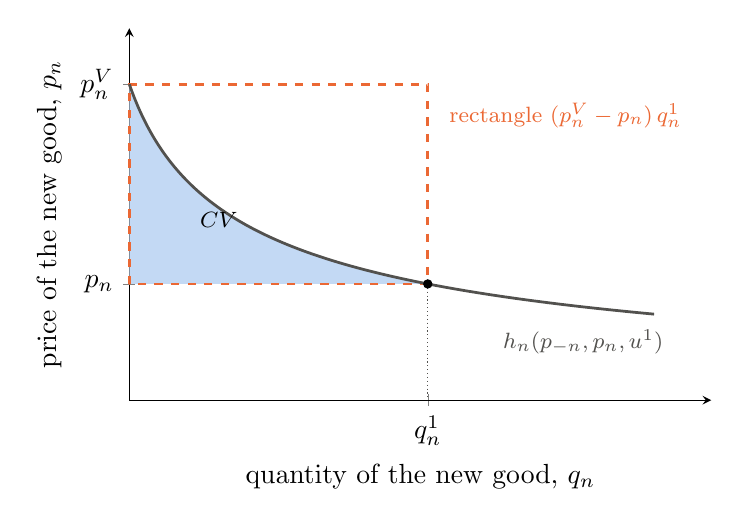
\begin{tikzpicture}
\begin{axis}[
  width=0.74\textwidth, height=0.52\textwidth,
  axis lines=left, xmin=0, xmax=1.95, ymin=0, ymax=3.2,
  xlabel={quantity of the new good, $q_n$}, ylabel={price of the new good, $p_n$},
  xtick={1}, xticklabels={$q_n^1$},
  ytick={1,2.71828}, yticklabels={$p_n$,$p_n^V$},
  every axis plot/.append style={line width=1pt},
  clip=false]
\addplot[draw=none, fill=c10p1blue!28, domain=1:2.71828, samples=80, variable=\t]
  ({(1-ln(\t))/\t},{\t}) -- (axis cs:0,2.71828) -- (axis cs:0,1) -- cycle;
\draw[dashed, c10p1orange, line width=1pt] (axis cs:0,1) rectangle (axis cs:1,2.71828);
\addplot[c10p1gray, domain=0.74:2.71828, samples=120, variable=\t] ({(1-ln(\t))/\t},{\t});
\draw[densely dotted, c10p1gray] (axis cs:1,1) -- (axis cs:1,0);
\fill (axis cs:1,1) circle (1.7pt);
\node[font=\footnotesize] at (axis cs:0.30,1.55) {$CV$};
\node[anchor=west, font=\footnotesize, text=c10p1orange] at (axis cs:1.04,2.45)
  {rectangle $(p_n^V - p_n)\,q_n^1$};
\node[anchor=west, font=\footnotesize, text=c10p1gray] at (axis cs:1.22,0.50)
  {$h_n(p_{-n},p_n,u^1)$};
\end{axis}
\end{tikzpicture}
\caption{The value of a new good. The curve is a compensated demand curve at the period-1 utility $u^1$. The
good sells at $p_n$, where the consumer buys $q_n^1$, and demand reaches zero at the virtual price $p_n^V$.
The shaded area is the compensating variation of \cref{prop:10-cv-newgood}. The dashed rectangle is the
Paasche bound of \cref{prop:10-index-bounds}. The curve drawn is $h_n = \frac{1 - \ln p_n}{p_n}$, so that
$p_n = q_n^1 = 1$ and $p_n^V = e$. The shaded area is $0.50$ and the rectangle is $1.72$.}
\label{fig:10-cv-area}
\end{figure}

\begin{remark}[Other prices, Marshallian surplus and Willig's approximation]\label{rem:10-willig}
If the prices of the other goods also change, from $p_{-n}^0$ to $p_{-n}^1$, the definition gives
$CV = e^R(p_{-n}^0,u^1) - e(p^1,u^1) = e\bigl(p_{-n}^0,p_n^V(p_{-n}^0,u^1),u^1\bigr) - y$. This is equation
(4) of \citet{Hausman1997} with all prices allowed to move, and \cref{sec:10-accounting} decomposes it. The
\emph{Marshallian surplus} of the new good is $CS = \int_{p_n}^{p_n^M}q_n(p_{-n},t,y)\,\dd t$. The argument
of \cref{prop:05-cv-ordering} applied on $[p_n,\infty)$ gives $EV \le CS \le CV$ for a normal good.
\citet{Willig1976} shows that the proportional gap $\frac{CV - CS}{CS}$ is approximately
$\frac{\bar\varepsilon_y\, CS}{2y}$ when the surplus is a small fraction of income, where $\bar\varepsilon_y$ is
the income elasticity of demand. His bounds replace $\bar\varepsilon_y$ by its smallest and largest values over the
price path. For a new good this path ends where the quantity reaches zero. If $\frac{\partial q_n}{\partial y}$
stays positive along the way, the income elasticity $\frac{\partial q_n}{\partial y}\frac{y}{q_n}$ grows without
bound, and the upper bound loses its force. \Cref{ex:10-linear-income} shows that the exact calculation is
easy in any case.

\citet[Section~7.4, pp.~184--188]{DeatonMuellbauer1980b} give a textbook account of these welfare measures. They
define both variations as differences of cost functions (their eqs.~4.1--4.2, p.~186). Our $CV$ is their
compensating variation for the move from $p^1$ back to $p^0$, the withdrawal of the good. They also explain why a
Marshallian area is not exact in general. It treats the marginal utility of income as constant, and that cannot
hold for all price changes (p.~185). For one good, the Hicksian and Marshallian demands coincide when utility is
quasi-linear in another good (Exercise~7.21, p.~189).
\end{remark}

\subsection{The cost-of-living index and the new-goods bias}\label{sec:10-col}

A cost-of-living index asks how much more, or less, income a consumer needs in period 1 to be as well off as
in period 0 \citep[p.~209]{Hausman1997}. \citet{Pollak1989} develops the theory.

\begin{definition}[Konüs cost-of-living index]\label{def:10-konus}
The \emph{cost-of-living index} between price vectors $p^0$ and $p^1$ at reference utility $u$ is
\begin{equation}\label{eq:10-konus}
  P(p^0,p^1,u) = \frac{e(p^1,u)}{e(p^0,u)}.
\end{equation}
\end{definition}

The index depends on the reference utility unless preferences are homothetic.
\citet[Section~7.1, pp.~170--173]{DeatonMuellbauer1980b} develop the index from the cost function. They show that
homotheticity is both necessary and sufficient for the index to be the same at every reference utility (p.~173).
With a new good the period-0
cost of reaching $u$ is $e^R(p_{-n}^0,u)$, which by \cref{lem:10-rothbarth}(c) equals
$e(p_{-n}^0,p_n^V,u)$. The period-0 price vector is therefore completed by the virtual price,
$p^0 = (p_{-n}^0,p_n^V(p_{-n}^0,u))$. With the period-1 reference and unchanged other prices,
\begin{equation}\label{eq:10-konus-newgood}
  P(p^0,p^1,u^1) = \frac{e(p_{-n},p_n,u^1)}{e(p_{-n},p_n^V,u^1)} = \frac{y}{y + CV} < 1 .
\end{equation}
The cost of living falls when a good is introduced. In the notation of \cref{lem:10-restricted}, the index is
$\frac{e(p,u^1)}{\tilde e(p,u^1,0)}$. Its reciprocal is the ratio of restricted to unrestricted cost, which
\citet[Exercise~7.16, p.~184]{DeatonMuellbauer1980b} propose as a measure of the cost of a ration.
\citet[p.~212]{Hausman1997} writes $y^*$ for
$e(p_{-n},p_n^V,u^1)$ and reports the reciprocal $\frac{y^*}{y}$, the cost of the period-1 standard of
living without the good relative to its cost with the good.

Statistical agencies compute \emph{matched-model} indexes. They compare the prices of goods sold in both
periods and add a new good to the sample only after it has been introduced. \citet[p.~210, n.~1]{Hausman1997}
notes that this procedure misses the gain at introduction, the welfare difference relative to a base period
in which the good was not sold. When the other prices do not change, every matched-model index equals one
between periods 0 and 1, whatever its formula. Comparing with \eqref{eq:10-konus-newgood},
\begin{equation}\label{eq:10-newgoods-bias}
  \frac{P^{MM}}{P(p^0,p^1,u^1)} - 1 = \frac{CV}{y},
\end{equation}
where $P^{MM} = 1$ is the matched-model index. The proportional overstatement of the price index equals the
value of the new good as a share of income. \citet[pp.~237--238]{Bresnahan1997} puts the point in terms of
timing. Official indexes link a new good in only after it has been sold for a while. They treat it as
irrelevant in its early stages, and the later the link, the larger the understatement of its value.

\subsection{Index-number bounds}\label{sec:10-bounds}

Index numbers built from observed prices and quantities bound the exact index. Let $q^0$ and $q^1$ be the
bundles bought in periods 0 and 1, with $q_n^0 = 0$ and $q_n^1 > 0$. Complete the period-0 prices with the
Hicksian virtual price at the period-1 utility, $p_n^0 = p_n^V(p_{-n},u^1)$. The \emph{Laspeyres} and
\emph{Paasche} indexes are
\begin{equation}\label{eq:10-LP}
  P_L = \frac{(p^1)^\top q^0}{(p^0)^\top q^0}, \qquad P_P = \frac{(p^1)^\top q^1}{(p^0)^\top q^1}.
\end{equation}
The Laspeyres index does not need $p_n^0$, because $q_n^0 = 0$. We write $w_n = \frac{p_nq_n^1}{y}$ for the
period-1 budget share of the new good.

\begin{proposition}[Index-number bounds for a new good]\label{prop:10-index-bounds}
Let Assumption~\ref{ass:10-prefs} hold, hold $p_{-n}$ and $y$ fixed, and suppose $p_n^V = p_n^V(p_{-n},u^1)$ is finite.
\begin{enumerate}[label=(\alph*)]
  \item The Laspeyres index records no change: $P_L = 1$.
  \item The Paasche index is $P_P = \frac{y}{y + (p_n^V - p_n)q_n^1}$.
  \item The exact index lies between them, $P_P \le P(p^0,p^1,u^1) \le P_L$. Equivalently,
  \begin{equation}\label{eq:10-cv-bounds}
    0 \le CV \le (p_n^V - p_n)\,q_n^1 .
  \end{equation}
  \item In share form, $\frac{CV}{y} \le w_n\Bigl(\frac{p_n^V}{p_n} - 1\Bigr)$.
\end{enumerate}
\end{proposition}

\begin{proof}
(a) Since $q_n^0 = 0$ and the other prices are unchanged,
$(p^1)^\top q^0 = \sum_{j\neq n}p_jq_j^0 = (p^0)^\top q^0$.

(b) The numerator is period-1 spending, $(p^1)^\top q^1 = y$. The denominator is
\begin{equation*}
  (p^0)^\top q^1 = \sum_{j\neq n}p_jq_j^1 + p_n^Vq_n^1 = y - p_nq_n^1 + p_n^Vq_n^1 = y + (p_n^V - p_n)q_n^1 .
\end{equation*}

(c) By \cref{prop:10-cv-newgood}, $CV = \int_{p_n}^{p_n^V}h_n(p_{-n},t,u^1)\,\dd t$. Hicksian demand is
nonnegative and nonincreasing in its own price, and $h_n(p_{-n},p_n,u^1) = q_n^1$ by \eqref{eq:10-duality}.
Hence, for every $t \in [p_n,p_n^V]$,
\begin{equation*}
  0 \le h_n(p_{-n},t,u^1) \le q_n^1 .
\end{equation*}
Integrating over $[p_n,p_n^V]$ gives \eqref{eq:10-cv-bounds}. Substituting the bounds into
\eqref{eq:10-konus-newgood} gives $P_P \le P \le 1 = P_L$.

(d) Divide \eqref{eq:10-cv-bounds} by $y$ and write $(p_n^V - p_n)q_n^1 = p_nq_n^1\bigl(\frac{p_n^V}{p_n} - 1\bigr)$.
\end{proof}

The Laspeyres bound is the matched-model index of \cref{sec:10-col}, and it says nothing. The Paasche bound is
the rectangle in \cref{fig:10-cv-area}. \citet[p.~212]{Hausman1997} describes the index-number approach of
Hicks and Rothbarth as measuring the change in real income by the ratio $\frac{p_n^Vq_n}{p_nq_n}$. The ratio
compares the value of the new good's purchases at the virtual price with their value at the actual price. Its
numerator minus its denominator is the rectangle. Hausman calls the approach approximately correct but notes
that it ignores the income compensation needed to stay on the indifference curve. \Cref{prop:10-index-bounds}
adds that the rectangle is an upper bound. Part (d) is the logic behind the rule of thumb that
\cref{sec:10-hausman} examines: the new good's share times the proportional gap between its virtual and
actual prices.

\begin{corollary}[Linear, convex and concave demand]\label{cor:10-half}
Under the conditions of \cref{prop:10-index-bounds}, if $h_n(p_{-n},t,u^1)$ is linear in $t$ on
$[p_n,p_n^V]$, then $CV = \frac{1}{2}(p_n^V - p_n)q_n^1$. If it is convex on that interval,
$CV \le \frac{1}{2}(p_n^V - p_n)q_n^1$. If it is concave, $CV \ge \frac{1}{2}(p_n^V - p_n)q_n^1$.
\end{corollary}

\begin{proof}
The chord joining $(p_n,q_n^1)$ and $(p_n^V,0)$ is $\ell(t) = q_n^1\frac{p_n^V - t}{p_n^V - p_n}$, and its
integral over $[p_n,p_n^V]$ is the triangle $\frac{1}{2}(p_n^V - p_n)q_n^1$. A linear function equals its
chord. A convex function lies below its chord between the two endpoints, and a concave function lies above
it. Integrating gives the three claims.
\end{proof}

\begin{remark}[The Konüs inequalities and a second-order view]\label{rem:10-konus}
Part (c) of \cref{prop:10-index-bounds} is a case of two inequalities due to \citet{Konus1939}.
\citet[Section~7.1, eqs.~1.3--1.4, p.~172]{DeatonMuellbauer1980b} give the standard proof. The bundle $q^1$ is one
way to reach $u^1$ at prices $p^0$, so it costs at least the minimum, $(p^0)^\top q^1 \ge e(p^0,u^1)$. Since
$(p^1)^\top q^1 = e(p^1,u^1)$,
\begin{equation*}
  P_P = \frac{(p^1)^\top q^1}{(p^0)^\top q^1} \le \frac{e(p^1,u^1)}{e(p^0,u^1)} = P(p^0,p^1,u^1).
\end{equation*}
The same argument with $q^0$ at prices $p^1$ gives $P_L \ge P(p^0,p^1,u^0)$. In general the two bounds apply at
different reference utilities, so the true index need not lie between them (p.~172). With a new good the
Laspeyres index equals one. \Cref{lem:10-rothbarth}(a) puts the true index below one at every reference utility.
This is why part (c) can bracket the index at the single reference $u^1$.

Deaton and Muellbauer also show that the Laspeyres index is a first-order approximation to the true index
(eqs.~1.6--1.7, p.~174). For a new good the first-order term is zero. Expand $t \mapsto e(p_{-n},t,u^1)$ to second
order around $p_n^V$. By Shephard's lemma its first derivative there is $h_n(p_{-n},p_n^V,u^1) = 0$, so
\begin{equation*}
  CV = e\bigl(p_{-n},p_n^V,u^1\bigr) - e\bigl(p_{-n},p_n,u^1\bigr)
  \approx -\frac{1}{2}\,\frac{\partial h_n}{\partial p_n}\,\bigl(p_n^V - p_n\bigr)^2 .
\end{equation*}
The value of a new good is thus a pure substitution effect, which an index with fixed base weights cannot capture.
If $h_n$ is linear on $[p_n,p_n^V]$, the expansion is exact. Substituting
$-\frac{\partial h_n}{\partial p_n} = \frac{q_n^1}{p_n^V - p_n}$ then gives $CV = \frac{1}{2}(p_n^V - p_n)q_n^1$, as
in \cref{cor:10-half}. Their first-order approximation to a compensating variation, the reference quantities times
the price changes (eq.~4.3, p.~187), is here the Paasche rectangle $(p_n^V - p_n)q_n^1$.
\end{remark}

\subsection{Separability: which demand curves are needed}\label{sec:10-separability}

Applying \cref{prop:10-cv-newgood} seems to require the whole expenditure function. \citet[p.~213,
n.~7]{Hausman1997} argues that under the usual separability assumptions only the demand curve for the new
good must be estimated. The next result makes the claim precise for homothetic separability, the first case
of Gorman's two-stage budgeting theorem (\cref{prop:05-first-stage}).

\begin{assumption}[Homothetic separability]\label{ass:10-hsep}
The goods are split into a group $N$ that contains good $n$ and the remaining goods. Utility is
$U(q) = F(q_{-N},\phi(q_N))$, where $F$ is strictly increasing in its last argument and the subutility $\phi$
is continuous, increasing, quasi-concave and homogeneous of degree one.
\end{assumption}

Let $P_N(p_N) = \min\{p_N^\top q_N : \phi(q_N) \ge 1\}$ be the unit cost of the subutility. It is the exact
price index of the group. Let $w_{n|N}(p_N) = \frac{\partial\ln P_N}{\partial\ln p_n}$ be the within-group
budget share of good $n$, which depends only on the prices of the group.

\begin{proposition}[New goods in a separable group]\label{prop:10-separable}
Under Assumptions~\ref{ass:10-prefs} and~\ref{ass:10-hsep}, the following hold.
\begin{enumerate}[label=(\alph*)]
  \item The expenditure function has the form $e(p,u) = E(p_{-N},P_N(p_N),u)$, where $E$ is the expenditure
  function for the goods outside $N$ and a composite good $Q_N = \phi(q_N)$ with price $P_N$.
  \item Fix $p_{-n}$ and $u$. Suppose the Hicksian demand for the composite is positive at every $p_n$ below the
  smallest $p_n$ at which $\frac{\partial P_N}{\partial p_n} = 0$. Then the Hicksian virtual price of good $n$ is
  that smallest $p_n$, and it depends only on the other prices of group $N$.
  \item Let $P_N^R = P_N(p_{N\setminus n},p_n^V)$ be the group index without the new good. Then
  \begin{equation}\label{eq:10-sep-index}
    \ln\frac{P_N^R}{P_N} = \int_{p_n}^{p_n^V}\frac{w_{n|N}(p_{N\setminus n},t)}{t}\,\dd t,
  \end{equation}
  \begin{equation}\label{eq:10-sep-cv}
    CV = E(p_{-N},P_N^R,u^1) - E(p_{-N},P_N,u^1) = \int_{P_N}^{P_N^R}H_N(p_{-N},\tau,u^1)\,\dd\tau,
  \end{equation}
  where $H_N = \frac{\partial E}{\partial P_N}$ is the Hicksian demand for the composite good.
\end{enumerate}
\end{proposition}

\begin{proof}
(a) Fix $u$ and minimize cost in two steps. Given a level $Q_N$ of the composite, the cheapest bundle with
$\phi(q_N) \ge Q_N$ costs $P_N(p_N)\,Q_N$, because $\phi$ is homogeneous of degree one. The consumer then
chooses $q_{-N}$ and $Q_N$ to minimize $p_{-N}^\top q_{-N} + P_NQ_N$ subject to $F(q_{-N},Q_N) \ge u$. The
value of this problem is $E(p_{-N},P_N,u)$.

(b) By Shephard's lemma and the chain rule,
\begin{equation*}
  h_n(p,u) = \frac{\partial E}{\partial P_N}\cdot\frac{\partial P_N}{\partial p_n} = H_N(p_{-N},P_N,u)\,\frac{\partial P_N}{\partial p_n}.
\end{equation*}
By hypothesis $H_N > 0$ below the first zero of $\frac{\partial P_N}{\partial p_n}$, so $h_n > 0$ there. At that
zero $h_n = 0$. The virtual price is therefore the first zero of $\frac{\partial P_N}{\partial p_n}$, a condition on
$p_N$ alone.

(c) Shephard's lemma applied to the unit cost gives $\frac{\partial\ln P_N}{\partial p_n} = \frac{w_{n|N}}{p_n}$.
Integrating in $p_n$ from $p_n$ to $p_n^V$ with the other group prices fixed gives \eqref{eq:10-sep-index}. For
\eqref{eq:10-sep-cv}, \eqref{eq:10-cv-e} and part (a) give
$CV = E(p_{-N},P_N^R,u^1) - E(p_{-N},P_N,u^1)$. Shephard's lemma for $E$ and the fundamental theorem of
calculus give the integral.
\end{proof}

The proposition splits the calculation into two stages. The change in the group index needs only the new good's
within-group share as a function of its own price, at the observed prices of the other goods in the group. In
that sense Hausman's claim holds. Part (b) needs its positivity condition. If the whole group can leave consumption,
$H_N$ can reach zero before $\frac{\partial P_N}{\partial p_n}$ does. The Hicksian virtual price is then the lower
price at which $H_N$ vanishes, and it can depend on $u$ and on prices outside the group. Part (c) still holds if we
evaluate $P_N^R$ at the first zero of $\frac{\partial P_N}{\partial p_n}$, because $E$ does not change with $P_N$
once $H_N = 0$. Converting the group index change into money needs the demand for the group
as a whole. If compensated group spending $X_N$ stays roughly constant over the relevant range, then
$CV \approx X_N\ln\frac{P_N^R}{P_N}$. The index used at the upper stage must be the exact group index with the
virtual price inserted for the period before the introduction. A Stone or matched-model index of the old
goods records no change. \citet[p.~221]{Hausman1997} rejects homotheticity of brand choice in his cereal
data. For groups that are not homothetic, two-stage budgeting holds only approximately or under the
generalized Gorman polar form of \cref{def:05-ggpf}. \citet{Gorman1959} gives the conditions.

\citet[Section~5.2, pp.~128--133]{DeatonMuellbauer1980b} give a textbook account of these conditions. The upper
stage allocates income across groups $G$ through group cost functions $c_G(u_G,p_G)$, subject to
$\sum_Gc_G(u_G,p_G) = y$ (their eqs.~2.11--2.14, p.~130). Gorman's first case has group cost functions of the form
$\theta_G(u_G)\,b_G(p_G)$, which is Assumption~\ref{ass:10-hsep} (eq.~2.15, p.~130). His second case is the generalized
polar form with utility additive across groups (eqs.~2.16--2.17, pp.~130--131). Weak separability also restricts substitution
across groups. For good $n$ in group $N$ and good $j$ in another group $H$, the compensated cross-price effect is
\begin{equation*}
  \frac{\partial h_n}{\partial p_j} = m_{NH}\,\frac{\partial q_n}{\partial y}\,\frac{\partial q_j}{\partial y},
\end{equation*}
where the scalar $m_{NH}$ depends only on the two groups (eq.~2.8, p.~128). A new good therefore reaches the
demand for a good in another group only through the expenditure allocated to that group.

\subsection{The CES variety-adjusted price index}\label{sec:10-feenstra}

Constant elasticity of substitution (CES) preferences give the best known correction of a price index for new
varieties \citep{Feenstra1994}. Let $\mathcal{I}_t$ be the set of varieties available in period $t$, with
taste parameters $a_j > 0$. The CES unit expenditure function is
\begin{equation}\label{eq:10-ces-unit}
  c(p;\mathcal{I}) = \Bigl(\sum_{j\in\mathcal{I}}a_jp_j^{1-\eta}\Bigr)^{\frac{1}{1-\eta}}, \qquad \eta > 1,
\end{equation}
and preferences are homothetic, so $e(p,u) = c(p;\mathcal{I})\,u$. Here $\eta$ is the elasticity of
substitution. \citet{Hausman1997} writes the CES utility function with a parameter $\rho$, and
$\eta = \frac{1}{1-\rho}$. \Cref{ch:aids} writes $\sigma$ for $\eta$, a symbol this chapter keeps for the
nesting parameter.

Shephard's lemma gives the expenditure shares. Differentiating \eqref{eq:10-ces-unit},
\begin{equation*}
  \frac{\partial c}{\partial p_j} = \frac{1}{1-\eta}\Bigl(\sum_k a_kp_k^{1-\eta}\Bigr)^{\frac{1}{1-\eta}-1}(1-\eta)a_jp_j^{-\eta}
  = c^{\eta}a_jp_j^{-\eta}.
\end{equation*}
The share of variety $j$ is therefore
\begin{equation}\label{eq:10-ces-share}
  w_j = \frac{p_j}{c}\frac{\partial c}{\partial p_j} = a_j\Bigl(\frac{p_j}{c}\Bigr)^{1-\eta}
  = \frac{a_jp_j^{1-\eta}}{\sum_{k\in\mathcal{I}}a_kp_k^{1-\eta}} .
\end{equation}

The first step handles a fixed set of varieties. For two positive numbers let
$\mathcal{L}(a,b) = \frac{a - b}{\ln a - \ln b}$ if $a \neq b$ and $\mathcal{L}(a,a) = a$. This is the
\emph{logarithmic mean}.

\begin{lemma}[Sato-Vartia index, \citealp{Sato1976,Vartia1976}]\label{lem:10-sato-vartia}
Let $\mathcal{I}$ be a set of varieties available in periods $t-1$ and $t$, with the same $a_j$ in both
periods. Let $\tilde w_{jt}$ be the share of variety $j$ in period-$t$ spending on $\mathcal{I}$. Then
\begin{equation}\label{eq:10-sv}
  \frac{c(p_t;\mathcal{I})}{c(p_{t-1};\mathcal{I})} = P^{SV}_{\mathcal{I}}
  \equiv \prod_{j\in\mathcal{I}}\Bigl(\frac{p_{jt}}{p_{j,t-1}}\Bigr)^{\omega_j}, \qquad
  \omega_j = \frac{\mathcal{L}(\tilde w_{jt},\tilde w_{j,t-1})}{\sum_{k\in\mathcal{I}}\mathcal{L}(\tilde w_{kt},\tilde w_{k,t-1})}.
\end{equation}
\end{lemma}

\begin{proof}
Write $c_t = c(p_t;\mathcal{I})$. Taking logs of \eqref{eq:10-ces-share} for the set $\mathcal{I}$ gives
$\ln\tilde w_{jt} = \ln a_j + (1-\eta)(\ln p_{jt} - \ln c_t)$. Differencing over time removes $\ln a_j$:
\begin{equation*}
  \Delta\ln\tilde w_j = (1-\eta)\bigl(\Delta\ln p_j - \Delta\ln c\bigr), \qquad j \in \mathcal{I}.
\end{equation*}
Solving for the change in the unit cost gives, for every $j$,
\begin{equation*}
  \Delta\ln c = \Delta\ln p_j - \frac{1}{1-\eta}\Delta\ln\tilde w_j .
\end{equation*}
Multiply by $\omega_j$ and sum over $j$. The weights sum to one, so
\begin{equation*}
  \Delta\ln c = \sum_{j\in\mathcal{I}}\omega_j\Delta\ln p_j - \frac{1}{1-\eta}\sum_{j\in\mathcal{I}}\omega_j\Delta\ln\tilde w_j .
\end{equation*}
By the definition of the logarithmic mean, $\mathcal{L}(\tilde w_{jt},\tilde w_{j,t-1})\Delta\ln\tilde w_j =
\tilde w_{jt} - \tilde w_{j,t-1}$. The shares sum to one in each period, so
$\sum_j\omega_j\Delta\ln\tilde w_j$ is proportional to $\sum_j(\tilde w_{jt} - \tilde w_{j,t-1}) = 0$. The
second term vanishes, and exponentiating gives \eqref{eq:10-sv}.
\end{proof}

The Sato-Vartia index uses only observed prices and quantities, and it is exact for CES preferences without
knowledge of $\eta$. New varieties enter through a second factor. Let $\mathcal{I} \subseteq
\mathcal{I}_{t-1}\cap\mathcal{I}_t$ be a nonempty set of varieties sold in both periods, with unchanged $a_j$.
Let $\lambda_t$ be the share of period-$t$ spending that goes to $\mathcal{I}$, and $\lambda_{t-1}$ the
corresponding share in period $t-1$:
\begin{equation*}
  \lambda_t = \frac{\sum_{j\in\mathcal{I}}p_{jt}q_{jt}}{\sum_{j\in\mathcal{I}_t}p_{jt}q_{jt}}, \qquad
  \lambda_{t-1} = \frac{\sum_{j\in\mathcal{I}}p_{j,t-1}q_{j,t-1}}{\sum_{j\in\mathcal{I}_{t-1}}p_{j,t-1}q_{j,t-1}}.
\end{equation*}

\begin{proposition}[CES index with changing varieties, \citealp{Feenstra1994}]\label{prop:10-feenstra}
Under CES preferences \eqref{eq:10-ces-unit},
\begin{equation}\label{eq:10-feenstra}
  \frac{c(p_t;\mathcal{I}_t)}{c(p_{t-1};\mathcal{I}_{t-1})}
  = P^{SV}_{\mathcal{I}}\,\Bigl(\frac{\lambda_t}{\lambda_{t-1}}\Bigr)^{\frac{1}{\eta-1}} .
\end{equation}
\end{proposition}

\begin{proof}
By \eqref{eq:10-ces-unit}, $\sum_{j\in\mathcal{I}}a_jp_{jt}^{1-\eta} = c(p_t;\mathcal{I})^{1-\eta}$ and
$\sum_{j\in\mathcal{I}_t}a_jp_{jt}^{1-\eta} = c(p_t;\mathcal{I}_t)^{1-\eta}$. Summing \eqref{eq:10-ces-share}
over $j \in \mathcal{I}$ gives the share of the common varieties,
\begin{equation*}
  \lambda_t = \frac{c(p_t;\mathcal{I})^{1-\eta}}{c(p_t;\mathcal{I}_t)^{1-\eta}} .
\end{equation*}
Solving for the full unit cost,
\begin{equation*}
  c(p_t;\mathcal{I}_t) = c(p_t;\mathcal{I})\,\lambda_t^{-\frac{1}{1-\eta}} = c(p_t;\mathcal{I})\,\lambda_t^{\frac{1}{\eta-1}} .
\end{equation*}
The same steps hold in period $t-1$. Taking the ratio of the two periods,
\begin{equation*}
  \frac{c(p_t;\mathcal{I}_t)}{c(p_{t-1};\mathcal{I}_{t-1})}
  = \frac{c(p_t;\mathcal{I})}{c(p_{t-1};\mathcal{I})}\Bigl(\frac{\lambda_t}{\lambda_{t-1}}\Bigr)^{\frac{1}{\eta-1}} .
\end{equation*}
\Cref{lem:10-sato-vartia} replaces the first ratio by $P^{SV}_{\mathcal{I}}$.
\end{proof}

A matched-model index computed on the common varieties is $P^{SV}_{\mathcal{I}}$. The second factor is the
correction for changing variety. When new varieties take a larger share of spending than the varieties that
disappear, $\lambda_t < \lambda_{t-1}$, and the correction lowers the index. The correction needs one
parameter, $\eta$. A low elasticity of substitution means a large correction, because the new varieties are
then poor substitutes for the old ones.

\begin{corollary}[One new variety]\label{cor:10-ces-newgood}
Suppose $\mathcal{I}_t = \mathcal{I}_{t-1}\cup\{n\}$, the other prices do not change, and the new variety
takes the share $w_n$ of period-$t$ spending. Then
\begin{equation}\label{eq:10-ces-newgood}
  \frac{c(p_t;\mathcal{I}_t)}{c(p_{t-1};\mathcal{I}_{t-1})} = (1 - w_n)^{\frac{1}{\eta-1}}, \qquad
  \frac{CV}{y} = (1 - w_n)^{-\frac{1}{\eta-1}} - 1, \qquad
  \frac{EV}{y} = 1 - (1 - w_n)^{\frac{1}{\eta-1}} .
\end{equation}
For small $w_n$ both measures are close to $\frac{w_n}{\eta - 1}$.
\end{corollary}

\begin{proof}
Take $\mathcal{I} = \mathcal{I}_{t-1}$. Unchanged prices give $P^{SV}_{\mathcal{I}} = 1$, and
$\lambda_{t-1} = 1$ and $\lambda_t = 1 - w_n$. \Cref{eq:10-feenstra} gives the first formula. Write
$c_0 = c(p_{t-1};\mathcal{I}_{t-1})$ and $c_1 = c(p_t;\mathcal{I}_t)$. Period-$t$ income is $y = c_1u^1$, and
the consumer would need $c_0u^1$ to reach $u^1$ without the new variety. Hence
$\frac{CV}{y} = \frac{c_0u^1 - c_1u^1}{c_1u^1} = \frac{c_0}{c_1} - 1$. Similarly, $y = c_0u^0$ and
$\frac{EV}{y} = \frac{c_0u^0 - c_1u^0}{c_0u^0} = 1 - \frac{c_1}{c_0}$. The approximation is the first-order
expansion of $(1 - w_n)^{\pm\frac{1}{\eta-1}}$ around $w_n = 0$.
\end{proof}

The formula for $CV$ is the removal formula of \cref{prop:05-variety}(a) read in reverse. Two features stand
out. First, CES demand is positive at every price, so the virtual price of the new variety is infinite. The
gain is nonetheless finite, because the CES demand curve approaches the price axis fast enough. Second, the
gain depends only on the new variety's share and on $\eta$. Nothing in the formula measures how close the new
variety is to particular old ones. \citet[p.~230]{Hausman1997} draws the conclusion that the CES, like the
logit, ``will tend to overvalue variety'' because it treats all goods symmetrically.

\begin{remark}[CES and logit]\label{rem:10-ces-logit}
The parallel with the logit model is exact. \Cref{sec:10-charspace} shows that adding a product with
post-introduction share $s_n$ to a logit market raises expected consumer surplus by
$-\frac{1}{\alpha}\ln(1 - s_n)$ per consumer. This is again a function of one share and one parameter
\citep{SmallRosen1981,McFadden1981}. \citet{AndersonDePalmaThisse1992} explain why, and
\citet[n.~29]{Hausman1997} cites them. Suppose each consumer buys one variety and spends all income on it,
with conditional indirect utility $\ln y - \ln p_j + \theta_j + \mu\epsilon_{ij}$ and type-I extreme value
$\epsilon_{ij}$. The logit choice probability is
$\Pr_j = \frac{e^{\frac{\theta_j}{\mu}}p_j^{-\frac{1}{\mu}}}{\sum_ke^{\frac{\theta_k}{\mu}}p_k^{-\frac{1}{\mu}}}$.
Each buyer of $j$ purchases $\frac{y}{p_j}$ units, so expected demand per consumer is
\begin{equation*}
  \frac{y\Pr_j}{p_j} = \frac{y\,e^{\frac{\theta_j}{\mu}}p_j^{-\frac{1}{\mu}-1}}{\sum_ke^{\frac{\theta_k}{\mu}}p_k^{-\frac{1}{\mu}}} .
\end{equation*}
This is the CES demand $\frac{y\,a_jp_j^{-\eta}}{\sum_ka_kp_k^{1-\eta}}$ implied by \eqref{eq:10-ces-share}, with
$\eta = 1 + \frac{1}{\mu}$ and $a_j = e^{\frac{\theta_j}{\mu}}$. Expected maximum utility is
$\ln y + \mu\ln\sum_ka_kp_k^{-\frac{1}{\mu}}$ plus a constant. Since $\mu(1-\eta) = -1$, this equals
$\ln y - \ln c(p;\mathcal{I})$ plus a constant, the CES indirect utility in logs. In both models each variety
carries its own taste shock, and the value of variety is built into the functional form.
\end{remark}

As an illustration, take two numbers from \citet{Hausman1997}. His reported CES elasticity is $\eta = 2.13$
(p.~231). His printed $\hat\rho = 0.580$ would imply 2.38, an inconsistency that \cref{sec:10-hausman-ces}
discusses. In addition, Apple-Cinnamon Cheerios had a 6.19 percent share of the family segment of ready-to-eat cereal in 1992
(Table 5.2). Treat the segment as a CES group. \Cref{cor:10-ces-newgood} then gives our computation
$(1 - 0.0619)^{\frac{1}{1.13}} = 0.945$.
The introduction lowers the segment's cost of living by 5.5 percent, and the compensating variation is 5.8
percent of segment spending. Hausman reports that his own CES specification gives a consumer surplus about
three times as large as his preferred estimate (p.~231). \Cref{sec:10-hausman} returns to the comparison.

\section{Functional form, extrapolation and bounds}\label{sec:10-functional}

The exact measures of \cref{sec:10-virtual} integrate the compensated demand curve from the observed price to
the virtual price. This section asks how much of that integral the data can deliver. We show that the answer
depends on the shape assumed beyond the data, and we compare three standard shapes. We then explain how to
recover the exact measure from an estimated Marshallian demand curve and derive a lower bound that needs only
convexity.

\subsection{The extrapolation problem}\label{sec:10-extrapolation}

Prices in a sample vary within a band around the observed price. In Hausman's cereal data the variation is on
the order of 50 percent, and prices as high as the estimated virtual price are never observed
\citep[p.~228]{Hausman1997}. His virtual price is about twice the actual price. The part of the area in
\cref{fig:10-cv-area} that lies above the highest observed price is then pinned down by the functional form
alone.

\citet[Section 1]{BerryPakes2007} make the general point. We rarely see demand for a new product at prices high
enough to estimate the reservation prices of many consumers without parametric assumptions. A demand system in
product space obtains the gains of inframarginal buyers by extending the curve estimated at low prices into a
higher price range. That extension can be very sensitive to the model. A demand system in characteristics
space also uses the price variation of products with similar characteristics. It therefore uses more
information, but similar problems arise. \Cref{sec:10-charspace} develops the characteristics approach.

The problem can be stated as a question of identification. Suppose the data reveal $h_n(p_{-n},t,u^1)$ for
$t \in [p_n,\bar p]$, with $\bar p$ the highest observed price and $h_n(p_{-n},\bar p,u^1) > 0$. Split the
compensating variation at $\bar p$:
\begin{equation}\label{eq:10-cv-split}
  CV = \underbrace{\int_{p_n}^{\bar p}h_n(p_{-n},t,u^1)\,\dd t}_{\text{supported by data}}
  + \underbrace{\int_{\bar p}^{p_n^V}h_n(p_{-n},t,u^1)\,\dd t}_{\text{extrapolated}} .
\end{equation}
Any nonincreasing extension of the demand curve beyond $\bar p$ agrees with the data. A curve that stays flat
at $h_n(p_{-n},\bar p,u^1)$ over a long interval before dropping to zero makes the second term as large as we
like. Without restrictions on shape, the data identify only the lower bound given by the first term. Bounds
that are more useful need restrictions, and point estimates need a functional form.

\subsection{Three canonical shapes}\label{sec:10-shapes}

Fix an observed point $(p,q)$ on the demand curve for good $n$. Let $\varepsilon = -\frac{p\,q'(p)}{q} > 0$
be the elasticity of demand at that point, written as a positive number as in the rest of the book. We compare
three demand curves that share the point and the slope. To keep the formulas transparent we integrate the
demand curve as drawn, and write $CS$ for the area.

\casehead{Linear demand}
Let $q(t) = a - bt$. Matching the slope gives $b = \frac{\varepsilon q}{p}$, and matching the point gives
$a = q + bp$. Demand reaches zero at
\begin{equation*}
  p^V = \frac{a}{b} = p + \frac{q}{b} = p\Bigl(1 + \frac{1}{\varepsilon}\Bigr).
\end{equation*}
The area is a triangle with height $p^V - p = \frac{q}{b}$ and base $q$:
\begin{equation*}
  CS = \int_p^{\frac{a}{b}}(a - bt)\,\dd t = \frac{(a - bp)^2}{2b} = \frac{q^2}{2b} = \frac{pq}{2\varepsilon}.
\end{equation*}

\casehead{AIDS demand with $\beta_n = 0$}
In the almost ideal demand system the budget share of good $n$ is linear in log prices. With $\beta_n = 0$ and
the other prices fixed, $w(t) = w + \gamma\ln\frac{t}{p}$, where $w$ is the observed share and $\gamma =
\gamma_{nn}$ (\cref{sec:05-aids}). Quantity is $q(t) = \frac{y\,w(t)}{t}$. The budget share does not depend on income, but quantity
has income elasticity one. Since $\ln q = \ln y + \ln w(t) -
\ln t$, the elasticity at $p$ is $\varepsilon = 1 - \frac{\gamma}{w}$. Hence $\gamma = -w(\varepsilon - 1)$,
which is negative when $\varepsilon > 1$. The share reaches zero where $\ln\frac{p^V}{p} = \frac{w}{-\gamma}$,
so
\begin{equation*}
  p^V = p\,\exp\Bigl(\frac{1}{\varepsilon - 1}\Bigr).
\end{equation*}
Substituting $x = \ln\frac{t}{p}$ and writing $x^V = \ln\frac{p^V}{p} = \frac{w}{-\gamma}$, the area is
\begin{equation*}
  CS = \int_p^{p^V}\frac{y\,w(t)}{t}\,\dd t = y\int_0^{x^V}(w + \gamma x)\,\dd x
  = y\Bigl(w\,x^V + \frac{\gamma\,(x^V)^2}{2}\Bigr) = \frac{y\,w^2}{2(-\gamma)} = \frac{pq}{2(\varepsilon - 1)}.
\end{equation*}
The last step uses $yw = pq$ and $-\gamma = w(\varepsilon - 1)$. With $\beta_n = 0$ the area also gives the
exact measure through $\ln(1 + \frac{CV}{y}) = \frac{CS}{y}$, which is \cref{prop:05-variety}(c).

\casehead{Constant-elasticity demand}
Let $q(t) = At^{-\varepsilon}$ with $A = qp^{\varepsilon}$. Demand is positive at every price, so $p^V = \infty$.
For $\varepsilon > 1$,
\begin{equation*}
  CS = \int_p^{\infty}At^{-\varepsilon}\,\dd t = \frac{Ap^{1-\varepsilon}}{\varepsilon - 1} = \frac{pq}{\varepsilon - 1}.
\end{equation*}
For $\varepsilon \le 1$ the integral diverges.

\Cref{tab:10-shapes} and \cref{fig:10-extrapolation} collect the three cases. Three lessons follow. First,
curves that agree on the level and slope of demand at the observed price give very different values. At
$\varepsilon = 2$ the constant-elasticity value is four times the linear one. Second, an infinite virtual price
does not imply an infinite gain. Third, both the AIDS and the constant-elasticity values explode as
$\varepsilon$ approaches one, while the linear value stays finite. The ratio of the constant-elasticity value
to the AIDS value is two at every elasticity. \citet[p.~231]{Hausman1997} finds a ratio of about three
between his CES and AIDS estimates.

\begin{table}[htbp]
\centering
\caption{Three demand curves through the same point}\label{tab:10-shapes}
\begin{threeparttable}
\begin{tabular}{@{}lcccc@{}}
\toprule
 & \multicolumn{2}{c}{General point $(p,q)$, elasticity $\varepsilon$} & \multicolumn{2}{c}{$p = q = 1$, $\varepsilon = 2$} \\
\cmidrule(lr){2-3}\cmidrule(lr){4-5}
Demand curve & Virtual price & Area $CS$ & Virtual price & Area $CS$ \\
\midrule
Linear & $p\bigl(1 + \frac{1}{\varepsilon}\bigr)$ & $\frac{pq}{2\varepsilon}$ & 1.50 & 0.25 \\[4pt]
AIDS with $\beta_n = 0$ & $p\exp\bigl(\frac{1}{\varepsilon - 1}\bigr)$ & $\frac{pq}{2(\varepsilon - 1)}$ & 2.72 & 0.50 \\[4pt]
Constant elasticity & $\infty$ & $\frac{pq}{\varepsilon - 1}$ & $\infty$ & 1.00 \\
\bottomrule
\end{tabular}
\begin{tablenotes}[flushleft]\footnotesize
\item Notes: Each curve passes through the observed point $(p,q)$ with own-price elasticity $\varepsilon > 1$,
written as a positive number. The area is the integral of the demand curve from $p$ to the virtual price. The
AIDS and constant-elasticity formulas require $\varepsilon > 1$. Derivations are in \cref{sec:10-shapes}, and
the numbers come from \texttt{figures/ch10/src/part1\_checks.py}.
\end{tablenotes}
\end{threeparttable}
\end{table}

\begin{figure}[htbp]
\centering
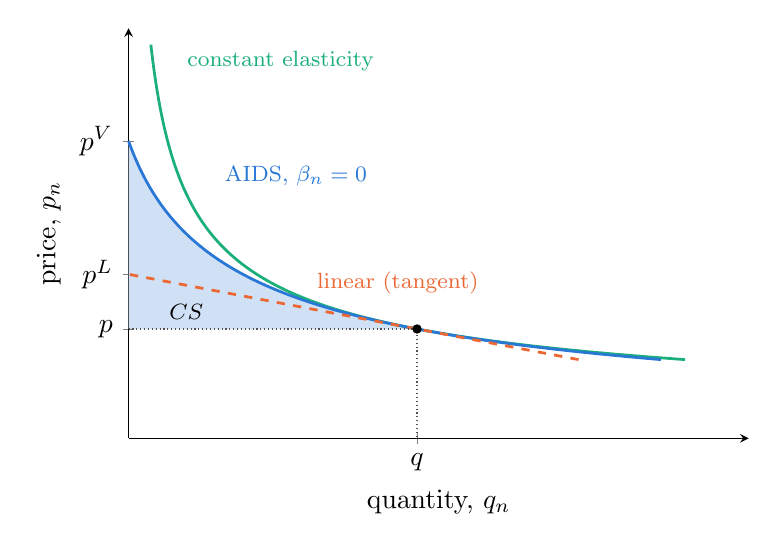
\begin{tikzpicture}
\begin{axis}[
  width=0.78\textwidth, height=0.56\textwidth,
  axis lines=left, xmin=0, xmax=2.15, ymin=0, ymax=3.75,
  xlabel={quantity, $q_n$}, ylabel={price, $p_n$},
  xtick={1}, xticklabels={$q$},
  ytick={1,1.5,2.71828}, yticklabels={$p$,$p^L$,$p^V$},
  every axis plot/.append style={line width=1pt},
  clip=false]
\addplot[draw=none, fill=c10p1blue!22, domain=1:2.71828, samples=80, variable=\t]
  ({(1-ln(\t))/\t},{\t}) -- (axis cs:0,2.71828) -- (axis cs:0,1) -- cycle;
\addplot[c10p1aqua, domain=0.72:3.6, samples=120, variable=\t] ({1/(\t*\t)},{\t});
\addplot[c10p1blue, domain=0.72:2.71828, samples=120, variable=\t] ({(1-ln(\t))/\t},{\t});
\addplot[c10p1orange, dashed, domain=0.72:1.5, samples=2, variable=\t] ({3-2*\t},{\t});
\draw[densely dotted, c10p1gray] (axis cs:0,1) -- (axis cs:1,1) -- (axis cs:1,0);
\fill (axis cs:1,1) circle (1.7pt);
\node[anchor=west, font=\footnotesize, text=c10p1aqua] at (axis cs:0.17,3.45) {constant elasticity};
\node[anchor=west, font=\footnotesize, text=c10p1blue] at (axis cs:0.30,2.40) {AIDS, $\beta_n = 0$};
\node[anchor=west, font=\footnotesize, text=c10p1orange] at (axis cs:0.62,1.42) {linear (tangent)};
\node[font=\footnotesize] at (axis cs:0.20,1.16) {$CS$};
\end{axis}
\end{tikzpicture}
\caption{Extrapolating demand beyond the data. All three curves pass through the observed point $(p,q) = (1,1)$
with own-price elasticity 2. The linear curve is the tangent at the observed point and reaches zero at
$p^L = 1.5$. The AIDS curve with $\beta_n = 0$ is convex and reaches zero at $p^V = e \approx 2.72$. The
constant-elasticity curve never reaches the price axis. The areas from $p$ upward are 0.25, 0.50 (shaded) and
1.00. Because the AIDS curve is convex, the tangent reaches zero below its virtual price, the bound of
\cref{prop:10-tangent}.}
\label{fig:10-extrapolation}
\end{figure}

With $\beta_n \neq 0$ the budget share of good $n$ varies with income, and the virtual price no longer has the closed form above.
The translog price index is quadratic in $\ln p_n$, so the zero-share condition is a quadratic equation in the
log virtual price \eqref{eq:05-virtual-quadratic}. The Hicksian condition \eqref{eq:05-virtual-hicks} needs a
one-dimensional root finder, and the compensating variation then follows from the closed form
\eqref{eq:05-cv-aids}. The AIDS represents preferences only where all shares are nonnegative, so the formulas
apply up to the virtual price and no further (\cref{sec:05-welfare-virtual}).

\subsection{Exact surplus from Marshallian demand*}\label{sec:10-exact}

Estimated demand systems are usually written in Marshallian form, with income as a regressor.
\citet{Hausman1981} shows how to recover the expenditure function from them. Along an indifference curve,
Shephard's lemma and the duality identity \eqref{eq:10-duality} give
\begin{equation}\label{eq:10-hausman-ode}
  \frac{\partial e(p,u)}{\partial p_n} = h_n(p,u) = q_n\bigl(p,e(p,u)\bigr).
\end{equation}
With the other prices fixed, this is an ordinary differential equation in $p_n$ for the function
$p_n \mapsto e(p,u)$. The constant of integration indexes utility, and the boundary condition
$e(p^1,u^1) = y$ selects the period-1 indifference curve. \citet[p.~212 and n.~6]{Hausman1997} describes this
step as solving the differential equation that arises from Roy's identity.

\begin{example}[Linear demand with income effects]\label{ex:10-linear-income}
Let $q_n = a + bp_n + cy$ with $b < 0$ and $c \neq 0$, and suppress the other prices. Then
\eqref{eq:10-hausman-ode} becomes
\begin{equation*}
  \frac{\dd e}{\dd p} - c\,e = a + bp .
\end{equation*}
Multiplying by the integrating factor $e^{-cp}$ turns the left side into an exact derivative:
\begin{equation*}
  \frac{\dd}{\dd p}\bigl(e^{-cp}e\bigr) = (a + bp)e^{-cp}.
\end{equation*}
An antiderivative of the right side is $-\frac{a + bp}{c}e^{-cp} - \frac{b}{c^2}e^{-cp}$. Differentiating it
gives $-\frac{b}{c}e^{-cp} + (a + bp)e^{-cp} + \frac{b}{c}e^{-cp} = (a + bp)e^{-cp}$, as required.
Integrating, with the constant of integration $u$ as the utility index,
\begin{equation}\label{eq:10-linear-e}
  e(p,u) = u\,e^{cp} - \frac{1}{c}\Bigl(bp + \frac{b}{c} + a\Bigr).
\end{equation}
We verify \eqref{eq:10-linear-e} directly. Its derivative is $\frac{\partial e}{\partial p} = cu\,e^{cp} -
\frac{b}{c}$. Substituting \eqref{eq:10-linear-e} into demand gives
\begin{equation*}
  a + bp + c\,e(p,u) = a + bp + cu\,e^{cp} - bp - \frac{b}{c} - a = cu\,e^{cp} - \frac{b}{c},
\end{equation*}
which equals the derivative. Setting $e(p,u) = y$ and solving gives the indirect utility function
$v(p,y) = e^{-cp}\bigl[y + \frac{1}{c}(bp + \frac{b}{c} + a)\bigr]$. Roy's identity returns $a + bp + cy$.

The Hicksian demand is $h(p,u) = cu\,e^{cp} - \frac{b}{c}$. Its slope is
$c^2u\,e^{cp} = c\bigl(h + \frac{b}{c}\bigr) = b + ch$, the Slutsky term $b + cq$ evaluated at $q = h$. We
assume it negative, so in this normalization the utility index $u$ is negative. At the observed point $(p^1,q^1)$ the identity
$h(p^1,u^1) = q^1$ gives $cu^1e^{cp^1} = q^1 + \frac{b}{c}$. The Hicksian virtual price solves
$cu^1e^{cp^V} = \frac{b}{c}$. Dividing the second condition by the first,
\begin{equation*}
  e^{c(p^V - p^1)} = \frac{b}{b + cq^1}, \qquad\text{so}\qquad p^V - p^1 = -\frac{1}{c}\ln\Bigl(1 + \frac{cq^1}{b}\Bigr).
\end{equation*}
At the virtual price demand is zero, so $a + bp^V + c\,e(p^V,u^1) = 0$ and $e(p^V,u^1) = -\frac{a + bp^V}{c}$.
The compensating variation is therefore
\begin{equation}\label{eq:10-linear-cv}
  CV = e(p^V,u^1) - y = -\frac{a + bp^V + cy}{c} = -\frac{q^1 + b(p^V - p^1)}{c}.
\end{equation}
The Marshallian choke price is $p^M = -\frac{a + cy}{b}$, so $p^M - p^1 = \frac{q^1}{-b}$, and the Marshallian
surplus is the triangle $CS = \frac{(q^1)^2}{2(-b)}$. Expanding the logarithm for small $c$ gives
$CV = \frac{(q^1)^2}{2(-b)} + \frac{c\,(q^1)^3}{3b^2}$ plus terms of order $c^2$. The second term is the
income-effect correction, positive for a normal good.

For numbers, take $p^1 = 1$, $y = 100$, $q^1 = 2$, $b = -2$ and $c = 0.02$, so $a = 2$ and the Slutsky term is
$-1.96$. The Marshallian choke price is 2.000 and $CS = 1.000$. The Hicksian virtual price is 2.010, and
\eqref{eq:10-linear-cv} gives $CV = 1.0135$. The equivalent variation, computed in the same way at the
period-0 utility, is $0.9934$. The income elasticity at the observed point is $\frac{cy}{q^1} = 1$, so
Willig's approximation of \cref{rem:10-willig} would suggest a gap of 0.5 percent between $CV$ and $CS$. The
exact gap is 1.35 percent, because the income elasticity rises without bound as the quantity falls to zero.
\end{example}

The same logic works without a parametric form. \citet{HausmanNewey1995} estimate demand nonparametrically and
solve \eqref{eq:10-hausman-ode} numerically, and they derive standard errors for the resulting exact surplus.
\citet[n.~24]{Hausman1997} uses their method for his estimates of exact consumer surplus and its asymptotic
standard error.

\subsection{A lower bound from convexity}\label{sec:10-tangent}

\citet[p.~228]{Hausman1997} proposes a bound that does not depend on the shape of demand near the price axis.
Draw the tangent to the demand curve at the observed price and see where it meets the price axis. If demand is
convex, the tangent lies below the curve, so it meets the axis below the virtual price.

\begin{proposition}[Tangent bound]\label{prop:10-tangent}
Let $q(t)$ be a demand curve for good $n$ (Marshallian at fixed income or Hicksian at fixed utility), with
$q(p) = q > 0$, differentiable at $p$ with $q'(p) < 0$, and convex on $[p,\infty)$. Let
$\varepsilon = -\frac{p\,q'(p)}{q}$ and
\begin{equation}\label{eq:10-pL}
  p^L = p + \frac{q}{-q'(p)} = p\Bigl(1 + \frac{1}{\varepsilon}\Bigr).
\end{equation}
Then (a) $p^L \le p^V$, and (b) the area $CS = \int_p^{p^V}q(t)\,\dd t$ satisfies
\begin{equation}\label{eq:10-tangent-cs}
  CS \ge \frac{1}{2}q\,(p^L - p) = \frac{pq}{2\varepsilon}.
\end{equation}
If in addition $p^V$ is finite, \cref{cor:10-half} gives $CS \le \frac{1}{2}q\,(p^V - p)$.
\end{proposition}

\begin{proof}
A convex function lies above its tangent lines. For every $t \ge p$,
\begin{equation*}
  q(t) \ge \ell(t) \equiv q + q'(p)(t - p),
\end{equation*}
and $\ell(p^L) = 0$ by \eqref{eq:10-pL}.

(a) Suppose $p^V < p^L$. Then $\ell(p^V) > 0 = q(p^V)$, which contradicts $q(t) \ge \ell(t)$. Hence
$p^L \le p^V$.

(b) Demand is nonnegative, so $q(t) \ge \max\{\ell(t),0\}$ for every $t \ge p$. Integrating over $[p,p^L]$
and using $p^L \le p^V$,
\begin{equation*}
  CS \ge \int_p^{p^L}q(t)\,\dd t \ge \int_p^{p^L}\ell(t)\,\dd t = \frac{1}{2}q\,(p^L - p)
  = \frac{1}{2}q\,\frac{q}{-q'(p)} = \frac{pq}{2\varepsilon}.
\end{equation*}
\end{proof}

The bound uses only the observed price, quantity and slope, and one shape restriction. The restriction is
weaker than a functional form, but it is still a restriction. Many common demand curves satisfy it. A linear
curve equals its tangent, so the bound is exact. A constant-elasticity curve has
$q''(t) = \varepsilon(\varepsilon + 1)At^{-\varepsilon-2} > 0$. For the AIDS with $\beta_n = 0$, differentiating
$q(t) = \frac{y\,w(t)}{t}$ twice gives
\begin{equation*}
  q'(t) = \frac{y\,(\gamma - w(t))}{t^2}, \qquad q''(t) = \frac{y\,(2w(t) - 3\gamma)}{t^3},
\end{equation*}
which is positive wherever $w(t) \ge 0$ and $\gamma < 0$. The demand curves that Hausman plots for his new
brand from his estimated AIDS are convex as well (his Figures 5.1 and 5.2). If demand were concave beyond the
data, the tangent would lie above the curve and would overstate the virtual price.

No convex curve through the observed point with the observed slope gives a smaller area, because every such
curve lies above the tangent line. In \cref{tab:10-shapes} the bound is the linear row, half the
AIDS value at $\varepsilon = 2$. Combined with \cref{cor:10-half}, convexity brackets the area between two
triangles. The lower one uses the tangent choke price $p^L$, and the upper one uses the true virtual price.
\citet[p.~228]{Hausman1997} applies the tangent construction to Apple-Cinnamon Cheerios and obtains lower-bound
virtual prices between about \$5.55 and \$5.94, about 65 percent above the average price of \$3.48.
\Cref{sec:10-hausman} examines these numbers.

\section{New goods under imperfect competition}\label{sec:10-imperfect}

The classical theory of \cref{sec:10-virtual} assumes perfect competition. The prices of the other goods stay
at marginal cost when the new good arrives \citep[p.~213]{Hausman1997}. In differentiated-product markets
this assumption fails in two ways. A firm that already sells close substitutes may reprice them once it owns
the new product. Rival firms face a new competitor and reprice their own products. Hausman notes the first
effect and quantifies it. \citet{Bresnahan1997} argues that the second effect is generally the more important
one. This section builds the welfare accounting that covers both, then studies each price response in turn.

\subsection{Welfare accounting with equilibrium prices}\label{sec:10-accounting}

Let $\mathcal{J}^1 = \mathcal{J}^0\cup\{n\}$ be the set of products in period 1. Firm $f$ owns the products in
$\mathcal{J}_f$, and firm $f^*$ introduces product $n$. Marginal costs $mc_j$ are constant, and the
introduction requires a fixed cost $F_n$. Market shares $s_j(p)$ come from a demand model with market size
$M$, and firms set prices in a Bertrand-Nash equilibrium. Let $\Delta(p)$ be the Jacobian of shares, the
matrix with $(j,r)$ element $\frac{\partial s_j(p)}{\partial p_r}$, and let $\Omega$ be the ownership matrix.
The first-order conditions are
\begin{equation}\label{eq:10-foc}
  s_j(p) + \sum_{r\in\mathcal{J}_f}(p_r - mc_r)\frac{\partial s_r(p)}{\partial p_j} = 0, \quad j\in\mathcal{J}_f,
  \qquad\text{or}\qquad s(p) + (\Omega\odot\Delta(p))^\top(p - mc) = 0 .
\end{equation}
This is the markup system of \cref{ch:diffprod}, solved as $p - mc = -[(\Omega\odot\Delta)^\top]^{-1}s$ as in
\eqref{eq:08-markup}.

Evaluating the welfare effect of an introduction that has already happened requires a counterfactual, because
the data show the market only with the new good. \citet[eqs.~1--3]{Petrin2002} uses the following steps.
\begin{enumerate}[label=(\roman*)]
  \item Estimate demand on data from the market with the new product, at observed prices $p^1$.
  \item Recover marginal costs from \eqref{eq:10-foc} at $p^1$: $mc = p^1 + [(\Omega\odot\Delta(p^1))^\top]^{-1}s(p^1)$.
  \item Solve \eqref{eq:10-foc} for the choice set $\mathcal{J}^0$, without product $n$, to obtain the
  counterfactual prices $p^0$ of the remaining products.
  \item Compute the compensating variation and the change in each firm's variable profit.
\end{enumerate}
In logit-type models, removing product $n$ is the same as raising its price to infinity, its virtual price. In
product-space systems, removal sets $p_n$ at its virtual price, which itself moves with the other prices.
The elasticities of the remaining products then follow \eqref{eq:05-rationed-elast}.

The compensating variation now has two parts. With $u^1$ the period-1 utility, add and subtract
$e^R(p_{-n}^1,u^1)$:
\begin{align}
  CV &= e^R(p_{-n}^0,u^1) - e(p^1,u^1) \nonumber\\
     &= \underbrace{e^R(p_{-n}^0,u^1) - e^R(p_{-n}^1,u^1)}_{\text{price effect}}
      + \underbrace{e^R(p_{-n}^1,u^1) - e(p^1,u^1)}_{\text{variety effect}} . \label{eq:10-cv-decomp}
\end{align}
The variety effect is the area of \cref{prop:10-cv-newgood}, evaluated at the period-1 prices of the other
goods:
\begin{equation*}
  e^R(p_{-n}^1,u^1) - e(p^1,u^1) = \int_{p_n^1}^{p_n^V(p_{-n}^1,u^1)}h_n(p_{-n}^1,t,u^1)\,\dd t .
\end{equation*}
The price effect values the change in the other prices for a consumer who cannot buy good $n$. The rationed
expenditure function is an ordinary expenditure function over the remaining goods, so Shephard's lemma
applies to it with the rationed Hicksian demands $h_k^R$. To first order,
\begin{equation}\label{eq:10-price-effect}
  e^R(p_{-n}^0,u^1) - e^R(p_{-n}^1,u^1) \approx \sum_{k\neq n}h_k^R(p_{-n}^1,u^1)\,(p_k^0 - p_k^1).
\end{equation}
The price effect is positive when the introduction lowers the other prices ($p_k^0 > p_k^1$), and negative when
it raises them. The decomposition is sequential, so its terms depend on the order in which the two changes
are made. \Cref{eq:05-cv-decomp} gives the analogous three-way decomposition of
\citet{ChaudhuriGoldbergJia2006} for product withdrawals.

The change in total welfare adds the change in profits and subtracts the fixed cost:
\begin{equation}\label{eq:10-dW}
  \Delta W = CV + \sum_f\bigl(\Pi_f^1 - \Pi_f^0\bigr) - F_n, \qquad
  \Pi_f^t = M\sum_{j\in\mathcal{J}_f}(p_j^t - mc_j)\,s_j(p^t).
\end{equation}
With heterogeneous consumers, $CV$ is the sum of the individual compensating variations. With quasi-linear
utility it equals the change in consumer surplus, and $\Delta W$ is the change in total surplus.

Both of the empirical studies of imperfect competition in this chapter fit this framework.
\citet[p.~234]{Hausman1997} starts from a variety effect of about \$32,000 per city and week. He then
subtracts \$4,605, a first-order price effect from the price increases of two existing Cheerios brands.
\citet[p.~720]{Petrin2002} computes the counterfactual equilibrium without minivans. In 1984, gains to buyers
of other vehicles from increased price competition account for almost 43 percent of total consumer benefits.
These gains are part of the price effect in \eqref{eq:10-cv-decomp}. \Cref{sec:10-hausman,sec:10-petrin}
develop both studies.

\subsection{Private and social returns}\label{sec:10-private-social}

A firm introduces a product when the introduction raises its own profit. The social value of the
introduction is $\Delta W$ in \eqref{eq:10-dW}. The two differ, and the gap governs whether markets supply too
many or too few products.

\begin{definition}[Private and social returns]\label{def:10-returns}
The \emph{private return} of the introduction is the change in the introducer's profit net of the fixed cost,
$G = \Pi_{f^*}^1 - \Pi_{f^*}^0 - F_n$. The \emph{social return} is $\Delta W$.
\end{definition}

Subtracting the definitions gives the general wedge,
\begin{equation}\label{eq:10-wedge-general}
  \Delta W - G = CV + \sum_{f\neq f^*}\bigl(\Pi_f^1 - \Pi_f^0\bigr).
\end{equation}
The introducer ignores the gain of consumers and the change in its rivals' profits. The next proposition
isolates the two terms when prices do not respond.

\begin{proposition}[The wedge at fixed prices]\label{prop:10-wedge}
Suppose utility is quasi-linear in income and the prices of all existing products are the same with and
without product $n$. Hicksian demand then does not depend on utility, and we write the variety effect as
$V_n = \int_{p_n}^{p_n^V}h_n(p_{-n},t)\,\dd t$, where $h_n$ is market Hicksian demand, the sum of the $M$
consumers' demands. Then
\begin{align}
  G &= M(p_n - mc_n)s_n^1 - M\sum_{k\in\mathcal{J}_{f^*}\setminus\{n\}}(p_k - mc_k)(s_k^0 - s_k^1) - F_n,
  \label{eq:10-private}\\
  \Delta W - G &= V_n - M\sum_{k\notin\mathcal{J}_{f^*}}(p_k - mc_k)(s_k^0 - s_k^1). \label{eq:10-wedge}
\end{align}
\end{proposition}

\begin{proof}
With prices fixed, each firm's profit changes only through its shares:
$\Pi_f^1 - \Pi_f^0 = M\sum_{k\in\mathcal{J}_f}(p_k - mc_k)(s_k^1 - s_k^0)$, with $s_n^0 = 0$. For the
introducer, split off product $n$ and subtract $F_n$ to obtain \eqref{eq:10-private}. The price effect in
\eqref{eq:10-cv-decomp} is zero, so $CV = V_n$. Substituting $CV = V_n$ and the rivals' profit changes into
\eqref{eq:10-wedge-general} gives \eqref{eq:10-wedge}.
\end{proof}

The wedge has two terms of opposite sign. The variety effect $V_n$ is surplus the introducer cannot
appropriate without perfect price discrimination, and it pushes toward too few products. The second term is
\emph{business stealing}: margins that rivals lose when their customers switch to the new product. It pushes
toward too many products. Cannibalization of the introducer's own products enters both the private and the
social return, so it is not part of the wedge at fixed prices. \citet{Spence1976} analyzes the two forces in
models of monopolistic competition. \citet{MankiwWhinston1986} show that business stealing alone produces
excessive entry under free entry in a homogeneous-good market, apart from the integer constraint. They also
show that product diversity can reverse the result (\cref{ch:theory}). \citet[p.~237, n.~1]{Bresnahan1997} quotes
\citet{EatonLipsey1989}, who conclude that ``we do not even know the nature of the bias'' between equilibrium
and optimal product diversity. The answer is empirical, and it needs estimates of both $V_n$ and the
diversion of customers from rivals.

\begin{remark}[Steep demand means large surplus and large rents]\label{rem:10-steep}
\citet[p.~243]{Bresnahan1997} observes that the condition for a large consumer gain, a steep demand curve for
the new product, is also the condition for a profitable single-product monopoly. A linear example makes this
exact. Let demand for the new product be $q = k(p^V - p)$, and let its seller have constant marginal cost
$mc_n < p^V$. The profit-maximizing price is $p^* = \frac{p^V + mc_n}{2}$, and the quantity is
$q^* = \frac{k(p^V - mc_n)}{2}$. Profit and consumer surplus at the optimum are
\begin{equation*}
  \pi^* = (p^* - mc_n)q^* = \frac{k(p^V - mc_n)^2}{4}, \qquad
  CS^* = \frac{1}{2}(p^V - p^*)q^* = \frac{k(p^V - mc_n)^2}{8} = \frac{\pi^*}{2}.
\end{equation*}
At the seller's optimum, consumer surplus and profit move in proportion. A demand estimate that implies a large
consumer gain also implies a large private return.
\end{remark}

\citet[pp.~245--246]{Bresnahan1997} organizes the effects of a new product under imperfect competition in a
two-by-two classification, reproduced in \cref{tab:10-bresnahan-2x2}. Columns give the channel, through the
introducer's other products or through competitors' products. Rows give the welfare criterion, the social
return or the inventor's private return. Bresnahan shades the price-discrimination cell, where Hausman's
analysis lies. He argues that the competition cell is generally far more important for the social return.

\begin{table}[htbp]
\centering
\caption{Imperfect competition and new goods}\label{tab:10-bresnahan-2x2}
\begin{threeparttable}
\begin{tabularx}{\textwidth}{@{}>{\raggedright\arraybackslash}p{2.3cm}>{\raggedright\arraybackslash}X>{\raggedright\arraybackslash}X@{}}
\toprule
 & Effect through the introducer's other products & Effect through competitors' products \\
\midrule
Social return & \textit{Price discrimination.} The introducer reprices its existing products now that it also
owns the new one. Consumers of those products gain or lose. This is the cell Hausman quantifies. &
\textit{Competition.} Rivals' residual demands become more elastic, and their prices typically fall.
Consumers of rival products gain. \\
\addlinespace
Inventor's private return & \textit{Cannibalization.} Part of the new product's sales comes from the
introducer's own products. The private return falls short of the new product's profit. &
\textit{Creative destruction.} Part of the new product's profit is taken from rivals' rents. It is a private
gain without a matching social gain. \\
\bottomrule
\end{tabularx}
\begin{tablenotes}[flushleft]\footnotesize
\item Notes: The cell labels are those of \citet[Figure 5C.2]{Bresnahan1997}, who shades the price-discrimination
cell. The descriptions are our reading of the labels, consistent with his text. The competition and
creative-destruction cells correspond to the price effect on rival products in \eqref{eq:10-cv-decomp} and to
the business-stealing term in \eqref{eq:10-wedge}.
\end{tablenotes}
\end{threeparttable}
\end{table}

\subsection{Multiproduct pricing in elasticity form}\label{sec:10-multiproduct}

Product-space demand systems deliver elasticities, so \citet{Hausman1997} writes the first-order conditions in
elasticity form. In this subsection $\varepsilon_{kj} = \frac{\partial q_k}{\partial p_j}\frac{p_j}{q_k}$ is
the signed elasticity of $q_k$ with respect to $p_j$. Own elasticities $\varepsilon_{jj}$ are negative, unlike
the positive scalar $\varepsilon$ of \cref{sec:10-functional}. Let $E$ be the matrix with $(k,j)$ element
$\varepsilon_{kj}$.

A firm sells products $1,\dots,K$ at constant marginal costs and maximizes
$\pi = \sum_{k=1}^K(p_k - mc_k)q_k(p)$. The derivative with respect to $p_j$ is
\begin{equation*}
  \frac{\partial\pi}{\partial p_j} = q_j + \sum_{k=1}^K(p_k - mc_k)\frac{\partial q_k}{\partial p_j}.
\end{equation*}
Let $R = \sum_kp_kq_k$ be the firm's revenue, $w_k = \frac{p_kq_k}{R}$ the revenue share of product $k$, and
$L_k = \frac{p_k - mc_k}{p_k}$ its Lerner index. Multiply the derivative by $\frac{p_j}{R}$. The first term
becomes $w_j$. Each term of the sum becomes
\begin{equation*}
  (p_k - mc_k)\frac{\partial q_k}{\partial p_j}\frac{p_j}{R}
  = \frac{p_k - mc_k}{p_k}\cdot\frac{p_kq_k}{R}\cdot\frac{\partial q_k}{\partial p_j}\frac{p_j}{q_k}
  = L_k\,w_k\,\varepsilon_{kj}.
\end{equation*}
Setting the derivative to zero gives equation (13) of \citet{Hausman1997}:
\begin{equation}\label{eq:10-foc-elast}
  \frac{p_j}{R}\frac{\partial\pi}{\partial p_j} = w_j + \sum_{k=1}^KL_k\,w_k\,\varepsilon_{kj} = 0, \qquad j = 1,\dots,K.
\end{equation}
For a single-product firm the condition reduces to $L_1 = -\frac{1}{\varepsilon_{11}}$, his equation (12).
Let $m_k = L_kw_k$ be the share-weighted margin and stack the conditions. In matrix form,
\begin{equation}\label{eq:10-foc-matrix}
  w + E^\top m = 0, \qquad m = -\bigl(E^\top\bigr)^{-1}w,
\end{equation}
which are his equations (14) and (15) with his $s$ renamed $w$ and his $w$ renamed $m$. The system is
\eqref{eq:05-foc-multi} in the notation of \cref{ch:aids}.

The elasticity form is the single-firm block of \eqref{eq:10-foc}. With one owner, $\Omega_{jr} = 1$ for all
products of the firm. Multiplying row $j$ of \eqref{eq:10-foc} by $\frac{Mp_j}{R}$ and using
$\frac{\partial s_r}{\partial p_j} = \varepsilon_{rj}\frac{s_r}{p_j}$ gives
$\frac{p_jq_j}{R} + \sum_r\frac{p_r - mc_r}{p_r}\frac{p_rq_r}{R}\varepsilon_{rj} = 0$, which is
\eqref{eq:10-foc-elast}.

Once margins are known with and without a product, constant marginal cost converts them into prices. From
$L_k = \frac{p_k - mc_k}{p_k}$ we get $p_k = \frac{mc_k}{1 - L_k}$, and therefore
\begin{equation}\label{eq:10-price-ratio}
  \frac{p_k^{\text{with}}}{p_k^{\text{without}}} = \frac{1 - L_k^{\text{without}}}{1 - L_k^{\text{with}}}.
\end{equation}
\Cref{sec:10-hausman} applies this formula to Hausman's Table 5.7. \citet[p.~241, n.~7]{Bresnahan1997} notes
that pricing equations of this kind imply an upward-sloping supply relation, which matters for the validity of
Hausman's instruments (\cref{sec:10-bresnahan}).

\subsection{The introducer's other prices}\label{sec:10-own-prices}

\citet[p.~231]{Hausman1997} gives the intuition for a price increase. Once the firm sells the new brand, part of
the demand it would lose by raising the price of an existing brand goes to the new brand instead of to rivals.
\citet[pp.~244--245]{Bresnahan1997} replies that \eqref{eq:10-foc-elast} changes in three ways when product
$K+1$ is added. First, a new positive term enters the sum,
\begin{equation*}
  \frac{p_{K+1} - mc_{K+1}}{p_{K+1}}\,w_{K+1}\,\varepsilon_{K+1,j} > 0,
\end{equation*}
which raises the marginal return to increasing $p_j$. Second, $w_j$ falls because the new product cannibalizes
product $j$. Third, $w_k$ falls for the firm's other existing products, which shrinks each positive cross term
$L_kw_k\varepsilon_{kj}$ with $k\neq j$. At fixed elasticities, the first effect pushes $p_j$ up. Bresnahan
treats the second and third, the falls in the shares, as the offsetting effects. At fixed margins and
elasticities only the third works this way. The terms in $w_j$ combine to $w_j(1 + L_j\varepsilon_{jj})$, which
is negative at the optimum when the firm's products are substitutes, so a smaller $w_j$ also pushes $p_j$ up.
The net effect on $p_j$ is ambiguous. Bresnahan adds that with linear demand and a two-product firm the effects offset exactly. The next
proposition proves this and extends it to any number of products.

\begin{proposition}[Linear demand: no repricing, \citealp{Bresnahan1997}]\label{prop:10-linear-offset}
A firm sells the products in $\mathcal{O} = \{1,\dots,K\}$ and can add product $n$. Demand for the $K+1$
products is $q = a - Bp$, with $B$ symmetric and positive definite, and marginal costs $mc$ are constant. The
prices of other firms are held fixed and absorbed into $a$. Before the introduction, demand for the products
in $\mathcal{O}$ is the rationed demand obtained by setting $p_n$ at its virtual price
$p_n^V(p_{\mathcal{O}}) = \frac{a_n - B_{n\mathcal{O}}p_{\mathcal{O}}}{b_{nn}}$. Then the profit-maximizing
prices of the products in $\mathcal{O}$ are the same with and without product $n$. In the two-product case
with $B = \bigl(\begin{smallmatrix} b & -d\\ -d & b\end{smallmatrix}\bigr)$, $b > d > 0$, the price of product
1 is in both cases
\begin{equation}\label{eq:10-linear-p1}
  p_1 = \frac{1}{2}\Bigl[\frac{ba_1 + da_2}{b^2 - d^2} + mc_1\Bigr].
\end{equation}
\end{proposition}

\begin{proof}
We compute the optimal prices before and after the introduction and compare them.

Before the introduction, substitute the virtual price into the demand for $\mathcal{O}$:
\begin{equation*}
  q_{\mathcal{O}} = a_{\mathcal{O}} - B_{\mathcal{O}\mathcal{O}}p_{\mathcal{O}} - B_{\mathcal{O}n}\,\frac{a_n - B_{n\mathcal{O}}p_{\mathcal{O}}}{b_{nn}}
  = \tilde a - \tilde Bp_{\mathcal{O}},
\end{equation*}
with
\begin{equation*}
  \tilde a = a_{\mathcal{O}} - \frac{B_{\mathcal{O}n}a_n}{b_{nn}}, \qquad
  \tilde B = B_{\mathcal{O}\mathcal{O}} - \frac{B_{\mathcal{O}n}B_{n\mathcal{O}}}{b_{nn}} .
\end{equation*}
The matrix $\tilde B$ is the Schur complement of $b_{nn}$ in $B$, so it is symmetric and positive definite.
Profit is $(p_{\mathcal{O}} - mc_{\mathcal{O}})^\top(\tilde a - \tilde Bp_{\mathcal{O}})$, a strictly concave
quadratic. Its gradient is
$\tilde a - \tilde Bp_{\mathcal{O}} - \tilde B^\top(p_{\mathcal{O}} - mc_{\mathcal{O}})$. Setting it to zero and
using symmetry gives $2\tilde Bp_{\mathcal{O}} = \tilde a + \tilde Bmc_{\mathcal{O}}$, so
\begin{equation*}
  p_{\mathcal{O}}^{\text{without}} = \frac{1}{2}\bigl(\tilde B^{-1}\tilde a + mc_{\mathcal{O}}\bigr).
\end{equation*}

After the introduction, the same steps with $a$ and $B$ give $p^{\text{with}} = \frac{1}{2}(B^{-1}a + mc)$.

The partitioned-inverse formula for a symmetric matrix gives the blocks of $B^{-1}$ in the rows of
$\mathcal{O}$:
\begin{equation*}
  (B^{-1})_{\mathcal{O}\mathcal{O}} = \tilde B^{-1}, \qquad (B^{-1})_{\mathcal{O}n} = -\frac{\tilde B^{-1}B_{\mathcal{O}n}}{b_{nn}} .
\end{equation*}
Hence
\begin{equation*}
  (B^{-1}a)_{\mathcal{O}} = \tilde B^{-1}a_{\mathcal{O}} - \frac{\tilde B^{-1}B_{\mathcal{O}n}a_n}{b_{nn}} = \tilde B^{-1}\tilde a,
\end{equation*}
and $p_{\mathcal{O}}^{\text{with}} = p_{\mathcal{O}}^{\text{without}}$.

In the two-product case, $B^{-1} = \frac{1}{b^2 - d^2}\bigl(\begin{smallmatrix} b & d\\ d & b\end{smallmatrix}\bigr)$,
so the first row of $\frac{1}{2}(B^{-1}a + mc)$ is \eqref{eq:10-linear-p1}. Directly, the virtual price is
$p_2^V = \frac{a_2 + dp_1}{b}$, and residual demand for product 1 is
$q_1 = \frac{ba_1 + da_2}{b} - \frac{b^2 - d^2}{b}p_1$. The monopoly price for this demand is half the sum of
its choke price $\frac{ba_1 + da_2}{b^2 - d^2}$ and $mc_1$, which is again \eqref{eq:10-linear-p1}.
\end{proof}

The result does not depend on the new product's intercept or marginal cost, which affect only whether it is
worth selling. The introduction is relevant when $q_n > 0$ at the optimal prices. With linear demand the
recapture effect is exactly offset by the cannibalization effects. The firm leaves its existing prices
unchanged, and the consumer gain from the introduction is the pure variety effect. Since rivals' prices are
held fixed in the proposition, the conclusion also applies to Hausman's own experiment. In a correctly computed
counterfactual, his price increases for existing Cheerios brands would have to come from the curvature of his
demand system. \Cref{sec:10-hausman-imperfect} shows that his calculation instead keeps the post-launch shares,
so it captures only the first of the three effects. Bresnahan
puts it this way: any tendency of one effect to dominate comes from ``higher-order derivatives,'' and the
paper contains no evidence on them \citep[p.~245]{Bresnahan1997}.

\begin{remark}[Logit demand: the existing prices rise]\label{rem:10-logit-multiproduct}
Curvature can push either way, and in the logit model it pushes prices up. Let firm $f$ sell the products in
$\mathcal{J}_f$ with logit demand and common price coefficient $\alpha$. With
$\frac{\partial s_j}{\partial p_j} = -\alpha s_j(1 - s_j)$ and $\frac{\partial s_k}{\partial p_j} = \alpha
s_ks_j$, the first-order condition \eqref{eq:10-foc} for $p_j$ becomes
\begin{equation*}
  s_j\Bigl[1 - \alpha(p_j - mc_j) + \alpha\sum_{k\in\mathcal{J}_f}(p_k - mc_k)s_k\Bigr] = 0 .
\end{equation*}
The bracket depends on $j$ only through $p_j - mc_j$. All the firm's products therefore carry the same markup
$\bar m$, and $\bar m = \frac{1}{\alpha(1 - S_f)}$ with $S_f$ the firm's total share. Write
$A_f = \sum_{k\in\mathcal{J}_f}e^{x_k\beta + \xi_k - \alpha mc_k}$ and let $R$ be the sum of $e^{\delta_k}$
over rival products, held fixed. Then
$1 - S_f = \frac{1 + R}{1 + R + A_fe^{-\alpha\bar m}}$, and the markup solves
\begin{equation*}
  \alpha\bar m\,(1 + R) = 1 + R + A_fe^{-\alpha\bar m}.
\end{equation*}
The left side rises with $\bar m$ and the right side falls, so the solution is unique. Adding a product raises
$A_f$, which raises the right side and hence the solution. Holding rivals' prices fixed, a logit firm raises the
prices of its existing products when it adds a product. For example, with $\alpha = 1$ and a single product
with $e^{x\beta + \xi - \alpha mc} = e^2$, a monopolist's markup is 2.00. Adding a second product with
$e^{1.5}$ raises the markup on both products to 2.25 (our computation).
Hausman's direction holds here, the linear case gives zero, and no general theorem signs the effect.
\end{remark}

\subsection{Rivals' prices}\label{sec:10-rival-prices}

Analyses of entry often hold rivals' prices fixed, and \citet[p.~244]{Bresnahan1997} argues that this is an
error (\cref{sec:10-bresnahan-competition}). The Bertrand concept has firms maximize profits taking one another's post-entry prices as
given. The analyst who evaluates entry must instead compute the new equilibrium, and in it rivals' prices
typically fall. Hausman's claim that his calculation gives a lower bound on the price changes, absent new entry
by competitors \citep[p.~233]{Hausman1997}, fails for this reason. The next proposition makes the competition
effect precise for single-product firms with logit demand.

\begin{proposition}[Entry lowers rivals' prices under logit]\label{prop:10-logit-rivals}
Consider single-product firms with logit demand
$s_j(p) = \frac{e^{v_j - \alpha p_j}}{1 + \sum_ke^{v_k - \alpha p_k}}$, with $v_j = x_j\beta + \xi_j$, constant
marginal costs $mc_j$ and $\alpha > 0$.
\begin{enumerate}[label=(\alph*)]
  \item Each firm's best response is unique, satisfies $(p_j - mc_j)\,\alpha\,(1 - s_j) = 1$, and is increasing
  in every rival's price.
  \item Let $p^0$ be an equilibrium without product $n$. Then the market with product $n$ has an equilibrium
  in which every incumbent's price is strictly below its value in $p^0$. If the equilibrium with product $n$ is
  unique, all incumbents' prices fall.
  \item In the symmetric case $v_j = v$ and $mc_j = mc$ for all $J$ products, the symmetric equilibrium markup
  is $p - mc = \frac{1}{\alpha(1 - s)}$, where $s$ is each product's share. The markup and the share both fall
  as $J$ rises, and the markup converges to $\frac{1}{\alpha}$ as $J \to \infty$.
\end{enumerate}
\end{proposition}

\begin{proof}
(a) Fix the rivals' prices and let $A_{-j} = 1 + \sum_{k\neq j}e^{v_k - \alpha p_k}$. Write the markup as
$m_j = p_j - mc_j$ and let $z_j = \frac{e^{v_j - \alpha mc_j}e^{-\alpha m_j}}{A_{-j}}$, so that
$s_j = \frac{z_j}{1 + z_j}$ and $1 - s_j = \frac{1}{1 + z_j}$. Profit is $Mm_js_j$, and the logit derivative
$\frac{\partial s_j}{\partial p_j} = -\alpha s_j(1 - s_j)$ gives
\begin{equation*}
  \frac{\partial(Mm_js_j)}{\partial p_j} = Ms_j\bigl[1 - \alpha m_j(1 - s_j)\bigr] = Ms_j\Bigl[1 - \frac{\alpha m_j}{1 + z_j}\Bigr].
\end{equation*}
The ratio $\frac{\alpha m_j}{1 + z_j}$ is zero at $m_j = 0$ and strictly increasing in $m_j$, because $z_j$
falls with $m_j$. The bracket therefore changes sign once, from positive to negative, and profit has a unique
maximum where
\begin{equation*}
  \alpha m_j = 1 + z_j = 1 + \frac{e^{v_j - \alpha mc_j}e^{-\alpha m_j}}{A_{-j}},
\end{equation*}
which is $(p_j - mc_j)\alpha(1 - s_j) = 1$. The left side increases in $m_j$ and the right side decreases. A
higher $A_{-j}$ lowers the right side and therefore lowers the solution. Since $A_{-j}$ falls when any rival
raises its price, the best response rises with every rival's price. The solution also satisfies
$m_j > \frac{1}{\alpha}$.

(b) Adding product $n$ adds the positive term $e^{v_n - \alpha p_n}$ to every incumbent's $A_{-j}$. Let
$\Phi$ be the best-response map of the market with product $n$, and start from $x^0 = (p^0,\Phi_n(p^0))$, the
old prices together with the entrant's best response to them. At $x^0$, each incumbent's $A_{-j}$ exceeds its
value at $p^0$ in the old market. By part (a), $\Phi_j(x^0) < p_j^0$ for every incumbent. Define
$x^{t+1} = \Phi(x^t)$. In the first step the incumbents' prices fall, while the entrant's price is unchanged
because $x_n^1 = \Phi_n(p^0) = x_n^0$. Hence $x^1 \le x^0$ componentwise. Because $\Phi$ is increasing,
$x^t \le x^{t-1}$ implies
$x^{t+1} = \Phi(x^t) \le \Phi(x^{t-1}) = x^t$. The sequence is therefore decreasing, and it is bounded below
by $mc + \frac{1}{\alpha}$. It converges to a limit $x^*$, which is a fixed point of $\Phi$ by continuity, so
$x^*$ is an equilibrium. For every incumbent, $x_j^* \le x_j^1 < p_j^0$. If the equilibrium is unique, it is
$x^*$.

(c) With symmetric products and a common markup $m$, let $x = e^{v - \alpha mc - \alpha m}$. Then
$s = \frac{x}{1 + Jx}$, and part (a) gives $m = \frac{1}{\alpha(1 - s)}$. Define
$g(m,J) = \alpha m(1 - s(m,J)) - 1$. Differentiating $s$,
\begin{equation*}
  \frac{\partial s}{\partial m} = -\frac{\alpha x}{(1 + Jx)^2} < 0, \qquad
  \frac{\partial s}{\partial J} = -\frac{x^2}{(1 + Jx)^2} < 0 .
\end{equation*}
Hence $\frac{\partial g}{\partial m} = \alpha(1 - s) - \alpha m\frac{\partial s}{\partial m} > 0$ and
$\frac{\partial g}{\partial J} = -\alpha m\frac{\partial s}{\partial J} > 0$. Since $g(0,J) = -1$ and
$g \to \infty$ as $m \to \infty$, the equation $g = 0$ has a unique root $m(J)$. The implicit function
theorem gives $\frac{\dd m}{\dd J} = -\bigl(\frac{\partial g}{\partial m}\bigr)^{-1}\frac{\partial g}{\partial J} < 0$. The markup
$\frac{1}{\alpha(1-s)}$ increases in $s$, so the equilibrium share falls as well. Finally $Js < 1$, so $s \to
0$ and $m(J) \to \frac{1}{\alpha}$ as $J \to \infty$.
\end{proof}

\Cref{tab:10-logit-entry} illustrates part (c) with $\alpha = 1$ and $v - \alpha mc = 2$. A single product
carries a markup of 2.00. With ten products the markup is 1.11, and it approaches the floor $\frac{1}{\alpha}
= 1$ slowly. The floor reflects the idiosyncratic logit taste shocks, which give every product a set of loyal
buyers, a feature \cref{sec:10-charspace} examines. Part (b) does not need symmetry. In an example with three
incumbents, $v = (2.0,1.5,1.0)$ and $mc = (1.0,0.8,0.5)$, the equilibrium prices are $(2.344,2.060,1.715)$.
Adding a fourth product with $v_n = 1.2$ and $mc_n = 0.7$ lowers them to $(2.287,2.016,1.678)$ (our
computation).

\begin{table}[htbp]
\centering
\caption{Symmetric logit equilibrium as the number of products grows}\label{tab:10-logit-entry}
\begin{threeparttable}
\begin{tabular}{@{}lccccccc@{}}
\toprule
Number of products $J$ & 1 & 2 & 3 & 5 & 10 & 20 & 50 \\
\midrule
Share of each product $s$ & 0.500 & 0.375 & 0.282 & 0.183 & 0.096 & 0.049 & 0.020 \\
Total inside share $Js$ & 0.500 & 0.749 & 0.846 & 0.916 & 0.961 & 0.981 & 0.993 \\
Markup $p - mc$ & 2.000 & 1.599 & 1.393 & 1.224 & 1.106 & 1.052 & 1.020 \\
\bottomrule
\end{tabular}
\begin{tablenotes}[flushleft]\footnotesize
\item Notes: Single-product firms with logit demand, $\alpha = 1$ and $v - \alpha mc = 2$ for every product. The
markup solves $p - mc = \frac{1}{\alpha(1 - s)}$ (\cref{prop:10-logit-rivals}). Our computation,
\texttt{figures/ch10/src/part1\_checks.py}.
\end{tablenotes}
\end{threeparttable}
\end{table}

The proof of part (b) also shows how the effect builds up. The first step of the iteration is the direct
response of each incumbent to the entrant. Later steps add the responses to the other incumbents' price cuts,
which push prices down further. \citet[p.~244, n.~13]{Bresnahan1997} makes this point: under Bertrand
competition the indirect effects of an introduction reinforce the direct effects. The monotone argument is an
instance of the theory of games with strategic complementarities \citep{MilgromRoberts1990}. Uniqueness of the
single-product logit equilibrium follows from the conditions of \citet{CaplinNalebuff1991}, discussed in
\cref{ch:diffprod}.

The logit model makes the competition effect unambiguous. Its own-price elasticity $-\alpha p_j(1 - s_j)$ rises
in magnitude whenever entry lowers $s_j$. Other demand systems allow exceptions. \citet[p.~243,
n.~12]{Bresnahan1997} notes that peculiar elasticities can reverse the result, for example when the new good
makes the demand curve for an old good steeper. One mechanism is a shift in the mix of buyers. If the entrant
draws away an incumbent's most price-sensitive customers, the remaining customers are less elastic, and the
incumbent's price can rise. \citet[p.~231, n.~32]{Hausman1997} concedes the counteracting effect. He writes
that the new brand can lower other firms' prices by raising the own-price elasticity of existing brands, and
that these interactions were beyond the reach of existing theory. Random-coefficient models permit both
outcomes. In \citet[p.~720]{Petrin2002}, station wagons have the largest percentage price decreases after the
minivan enters, and large family sedans the largest dollar decreases, of \$100 to \$150
(\cref{sec:10-petrin}).

The value of a new good under imperfect competition is therefore the variety effect at the new prices plus
the price effects on all other products. The effect through the introducer's own products has no general
sign. It is zero with linear demand, positive with logit demand, and determined in any application by the
curvature of the estimated demand system. The effect through rivals' products usually benefits consumers, and
it can be large. The case studies that follow measure these effects with actual data. The first,
\citeauthor{Hausman1997}'s valuation of a new breakfast cereal, applies every tool of
\cref{sec:10-virtual,sec:10-functional} and the multiproduct pricing of this section. The critique of
\citet{Bresnahan1997} then turns on the competition effect and on the instruments behind the demand estimates.

\section{Case study: Apple-Cinnamon Cheerios (Hausman 1997)}\label{sec:10-hausman}

\citet{Hausman1997} is an early study that values a single new brand with an estimated
demand system for differentiated products. It applies the virtual-price theory of \cref{sec:10-virtual} to the ready-to-eat
(RTE) cereal industry. It then adds the multiproduct pricing adjustment that \cref{sec:10-imperfect}
analyzes in general form. We take the paper in the order question, setting, data, model, identification,
results, robustness, interpretation and critique.\footnote{The NBER page of the volume is dated January
1996, so the paper is sometimes cited as Hausman (1996). Page numbers below are those of the published
volume, pp.~209--237.} \Cref{sec:10-bresnahan} then examines the comment by \citet{Bresnahan1997}, published
with the paper, which disputes both the instruments and the treatment of competition.

The paper uses several symbols that this book reserves for other objects, so we rename them. Hausman's
revenue share $s$ becomes $w$, and his margin-weighted share $w$ becomes $m$. His cost coefficient $\delta_j$
becomes $\kappa_j$, and his segment price coefficients $\delta_k$ become $b_{mg}$. His segment price indexes
$\pi_{knt}$ become $P_{gnt}$, his virtual price $p_n^*$ becomes $p_n^V$, and his elasticity $e_{kj}$ becomes
$\varepsilon_{kj}$. As in \cref{sec:10-imperfect}, elasticities in this section are signed, so own-price
elasticities are negative.

\subsection{The question}\label{sec:10-hausman-question}

Hausman asks three questions (pp.~209--210). How much consumer surplus does one incremental brand create?
By how much does the consumer price index (CPI) overstate cereal inflation because it ignores new brands?
How does multiproduct pricing by the introducing firm change the answer?

The second question motivates the first. The Bureau of Labor Statistics includes a new good in the CPI only
after it has been on sale for some time (fn.~1). The index then tracks the good's later price changes but
never records the gain from its arrival. In the terms of \cref{sec:10-virtual}, the exact index values the
new good in the base period at its virtual price, while the CPI drops the good from the base-period
comparison. Hausman quotes the agency's own warning that a systematic measurement error of this kind would
bias the measured rate of price change \citep[p.~210, quoting][]{Fixler1993}.

The question also matters for the economics of product differentiation. Hausman notes that differentiation is
one of the two basic business strategies (p.~209). He calls RTE cereal ``perhaps the foremost industry in the
introduction of new goods'' (p.~213). Some economists read cereal brand
proliferation as wasteful or as a device to deter entry \citep{Schmalensee1978}. If new brands create
little surplus, the advertising spent to launch them is mostly a private transfer. If they create large
surplus, official price indexes miss a real gain. Hausman chooses a demanding test case. Apple-Cinnamon
Cheerios (ACC), introduced by General Mills in 1989, sits next to two established brands of the same firm,
Cheerios and Honey-Nut Cheerios. Whether consumers value a product that may already be ``spanned by existing
brands'' is an empirical question (p.~216).

\subsection{The setting: brand proliferation in ready-to-eat cereal}\label{sec:10-hausman-setting}

The industry introduces many brands (pp.~213--215). From 1980 to 1992 about 190 new brands
entered a pool of about 160 existing ones. More than 95 of the new brands were discontinued. Of the 27
brands introduced in 1989, 14 had been withdrawn by 1993. Only 2 of the 190 reached a pound share above
1 percent. Even so, about 25 percent of RTE consumption came from brands introduced within the previous ten
years. Hausman notes that about 80 percent of new consumer products fail in general (fn.~9).

The industry is concentrated at the firm level and fragmented at the brand level. Six firms together
accounted for 94 percent or more of dollar sales over 1982--92 (p.~214). Kellogg's share ranged from 37.3 to
41.5 percent, General Mills' from 23.0 to 29.0 percent and General Foods' (Post) from 10.4 to 15.8 percent.
Quaker, Ralston and Nabisco each held about 3.0 to 8.9 percent, and Malt-O-Meal was the only other firm
above 1 percent. Individual brands are small. In 1993 the largest General Mills brand, Cheerios, had 5.3
percent, and the largest Kellogg brands, Frosted Flakes and Corn Flakes, had 5.0 and 4.99 percent (p.~214).

No significant manufacturer had entered successfully in fifty years. Entrants of the 1970s, such as
Pillsbury, Pet and Colgate, did not last, although real revenue grew by 6.7 percent a year over 1982--92
(p.~215). Launching a brand cost \$20--40 million in advertising and promotion in the first year, and the
spending typically continued for one or two more years. A 1 percent share counts as ``a great success''
(p.~215). The only outside competition of note came from private labels, which doubled their share from
about 4 to 8 percent over five to ten years. Ralston manufactured most of them.

Hausman rejects the view that proliferation deters entry. The Federal Trade Commission had argued this
``shared monopoly'' theory against the leading firms and lost (fn.~10). \citet{Judd1985} showed that
proliferation is a credible preemption device only if exit costs are high, and withdrawing a brand is cheap.
Hausman instead sees sunk advertising as the main barrier to entry, in the spirit of \citet{Sutton1991}. The
success of private labels, which advertise little and copy existing brands, supports this reading
(pp.~215--216). The welfare question remains open under either view. Many economists doubt the social value
of brands that mostly fail, and ACC is a natural test.

\subsection{Data}\label{sec:10-hausman-data}

The data are Nielsen Scantrak scanner data (p.~220). The time series has 137 weekly observations from
January 1990 to August 1992. The cross section has seven metropolitan areas: Boston, Chicago, Detroit,
Los Angeles, New York, Philadelphia and San Francisco. In each area Nielsen samples supermarkets by
stratified random sampling, and the sample covers most cereal sold. Sales are recorded for each stock-keeping
unit (each package size of each brand) at a weekly average price. Hausman aggregates packages to weekly
pounds of each brand and an average price per pound. The panel thus has $7 \times 137 = 959$ city-week
observations for each brand. Prices vary by about 50 percent over the sample, mostly through promotions and
coupons (pp.~216 and 228).

Brands are grouped into three segments used by industry marketing analysts (Table 5.1). The adult segment
contains Shredded Wheat Squares, Special K, Fruit Wheats, Shredded Wheat, Shredded Wheat and Bran,
Spoon-Size Shredded Wheat and Grape Nuts. The child segment contains Trix, Kix, Frosted Flakes and Froot
Loops. The family segment contains the nine brands of \cref{tab:10-hausman-desc}, ACC among them. The family
segment accounts for about 26.4 percent of RTE sales (p.~220). Hausman reports that his specification tests
do not reject the segmentation (fn.~22).

\begin{table}[htbp]
\centering
\caption{The family segment of ready-to-eat cereal, 1992}\label{tab:10-hausman-desc}
\begin{threeparttable}
\begin{tabular}{@{}llcc@{}}
\toprule
Brand & Company & \makecell{Average price\\(\$ per pound)} & \makecell{Segment share\\(percent)} \\
\midrule
Cheerios                & General Mills & 2.644 & 21.62 \\
Honey-Nut Cheerios      & General Mills & 3.605 & 15.03 \\
Apple-Cinnamon Cheerios & General Mills & 3.480 & \phantom{0}6.19 \\
Corn Flakes             & Kellogg       & 1.866 & 14.24 \\
Raisin Bran             & Kellogg       & 3.214 & 13.11 \\
Rice Krispies           & Kellogg       & 2.475 & 13.54 \\
Frosted Mini-Wheats     & Kellogg       & 3.420 & \phantom{0}9.07 \\
Frosted Wheat Squares   & Nabisco       & 3.262 & \phantom{0}1.48 \\
Raisin Bran             & Post          & 3.046 & \phantom{0}5.72 \\
\bottomrule
\end{tabular}
\begin{tablenotes}[flushleft]\footnotesize
\item Notes: Reproduced in full from \citet[Table 5.2]{Hausman1997}. Shares are shares of family-segment
sales. The three Cheerios brands together hold 42.84 percent of the segment.
\end{tablenotes}
\end{threeparttable}
\end{table}

The three Cheerios brands hold 42.84 percent of the family segment, or about 11.3 percent of all cereal
sales (p.~221). ACC holds 6.19 percent of the segment, about 1.6 percent of all cereal. By the standards of
\cref{sec:10-hausman-setting} the brand is a large success, since almost no new brand reaches 1 percent.

\subsection{A three-level demand system}\label{sec:10-hausman-model}

Hausman estimates demand with the multistage budgeting structure of \cref{sec:05-separability}, drawn in
\cref{fig:05-budget-tree}(a). The top level is total cereal demand. The middle level allocates cereal
spending across segments. The bottom level allocates segment spending across brands. Estimation proceeds
from the bottom up, and the price indexes of each level feed the level above (pp.~216--218). We index
segments by $m$ and $g$, brands by $i$ and $j$, cities by $n = 1,\dots,N$ and weeks by $t = 1,\dots,T$. In
this section $N = 7$ counts cities, not firms, and $M$ counts segments, not consumers. The subscript $n$ on
$p_n^V$ and $w_n$ still denotes the new good.

\casehead{Bottom level}
For brand $i$ in segment $m$, the share equation is an almost ideal demand system (AIDS) in segment
expenditure \citep{DeatonMuellbauer1980a},
\begin{equation}\label{eq:10-h-bottom}
  w_{int} = \alpha_{in} + \beta_i\ln\frac{Y_{mnt}}{P_{mnt}} + \sum_{j\in m}\gamma_{ij}\ln p_{jnt} + \xi_{int}
\end{equation}
(Hausman's eq.~5). Here $w_{int}$ is the revenue share of brand $i$ in segment spending $Y_{mnt}$, and
$P_{mnt}$ is the segment price index. The price per pound of brand $j$ is $p_{jnt}$, and $\xi_{int}$ is the
demand error. The intercept $\alpha_{in}$ is a brand-city effect. Table 5.3 shows that the equations also
include a quadratic time trend and a display variable $\ln(DISP + 1)$. Adding up across the brands of the
segment requires $\sum_i\alpha_{in} = 1$, $\sum_i\beta_i = 0$ and $\sum_i\gamma_{ij} = 0$. Homogeneity requires
$\sum_j\gamma_{ij} = 0$, and Slutsky symmetry requires $\gamma_{ij} = \gamma_{ji}$.

Three features of \eqref{eq:10-h-bottom} carry the analysis. First, the $\gamma_{ij}$ are unrestricted apart
from symmetry and homogeneity. With nine brands that leaves $\frac{9\times 8}{2} = 36$ free price coefficients,
and no equal-cross-elasticity assumption constrains substitution within the segment. Second, a test of
$\beta_i = 0$ for all $i$ is a test of \emph{segment homotheticity}, the hypothesis that brand shares do not
depend on segment spending. Third, the expenditure variable is segment spending. Using total spending ``is
inconsistent with the economic theory of multistage budgeting'' and gives worse results (p.~217).

The \emph{conditional elasticities} hold segment spending fixed. With the translog index of the AIDS,
Shephard's lemma gives $\frac{\partial\ln P_{m}}{\partial\ln p_j} = w_{j|m} - \beta_j\ln\frac{Y_m}{P_m}$, where
$w_{j|m}$ is brand $j$'s share of the segment. Since $q_i = \frac{w_{i|m}Y_m}{p_i}$, we have
$\ln q_i = \ln w_{i|m} + \ln Y_m - \ln p_i$. Differentiating with respect to $\ln p_j$ at fixed $Y_m$,
\begin{align}
  \varepsilon^c_{ij} &= -\indic\{i = j\} + \frac{1}{w_{i|m}}\frac{\partial w_{i|m}}{\partial\ln p_j}\notag\\
  &= -\indic\{i = j\} + \frac{\gamma_{ij} - \beta_i\bigl(w_{j|m} - \beta_j\ln\frac{Y_m}{P_m}\bigr)}{w_{i|m}}.
  \label{eq:10-h-cond-elast}
\end{align}
Differentiating instead with respect to $\ln Y_m$ gives the conditional expenditure elasticity
$\phi_{i|m} = 1 + \frac{\beta_i}{w_{i|m}}$. These are the AIDS formulas of \cref{sec:05-aids-elasticities},
written with within-segment shares.

\casehead{Middle level}
Segment quantities follow a log-log system,
\begin{equation}\label{eq:10-h-middle}
  \ln q_{mnt} = \alpha_{mn} + \phi_m\ln Y_{nt} + \sum_{g=1}^{M}b_{mg}\ln P_{gnt} + \xi_{mnt}, \qquad m = 1,\dots,M
\end{equation}
(Hausman's eq.~6). Here $q_{mnt}$ is the pound volume of segment $m$, $Y_{nt}$ is total cereal spending in
the city-week, and $P_{gnt}$ is the price index of segment $g$. Because cereal spending is held fixed,
$\phi_m$ is the segment's expenditure elasticity and $b_{mg}$ are price elasticities conditional on cereal
spending. Hausman uses Stone indexes at this level (p.~221) and states that the choice between exact and
Stone indexes typically matters little (p.~218). Exact two-stage budgeting requires additive separability at the level above, and the
AIDS is a generalized Gorman polar form, so Gorman's theorem applies \citep[fn.~17]{Hausman1997}. A less
restrictive middle level, not consistent with exact two-stage budgeting, gives similar results (fn.~17).
The log-log system is second-order flexible, and Slutsky restrictions are not imposed on it (fn.~18).

\casehead{Top level}
Total cereal consumption $Q_t$ satisfies
\begin{equation}\label{eq:10-h-top}
  \ln Q_t = a_0 + a_1\ln y_t + \varepsilon_U\ln\Pi_t + Z_t\psi + \xi_t
\end{equation}
(Hausman's eq.~7), where $y_t$ is real disposable income, $\Pi_t$ is the real cereal price index and $Z_t$
holds demographic and monthly seasonal variables. A longer period than store data provide helps to estimate
this elasticity, so Hausman fits \eqref{eq:10-h-top} to sixteen years of national monthly data from the Bureau
of Labor Statistics. He uses
instrumental variables, with cost shifters for ingredients, packaging and labor as instruments (p.~218). The
coefficient $\varepsilon_U$ is the price elasticity of total cereal demand.

\casehead{Combining the levels}
Pricing and welfare calculations need \emph{unconditional} elasticities, which let segment and cereal
spending respond to prices. The next result writes them in terms of the three levels. It is the formula of
\eqref{eq:05-hlz-uncond} for beer, restated in this section's notation with Stone indexes. We restate it
because its rank-one structure matters for reading Hausman's tables.

\begin{proposition}[Unconditional elasticities in a three-level system]\label{prop:10-elasticity-aggregation}
Let brand $i$ belong to segment $m$ and brand $j$ to segment $g$. Assume the following.
\begin{enumerate}[label=(\roman*)]
\item The demand $q_i$ depends on prices only through the prices of segment $m$ and on spending only through
$Y_m$, with elasticities $\varepsilon^c_{ij}$ and $\phi_{i|m}$.
\item Segment spending is $Y_m = P_mq_m$, with a Stone index satisfying
$\frac{\partial\ln P_g}{\partial\ln p_j} = w_{j|g}$.
\item Segment quantities follow \eqref{eq:10-h-middle}.
\item Cereal spending is $Y = \Pi Q$, with $\ln\Pi = \sum_g w_g\ln P_g$ and $w_g$ segment $g$'s share of cereal
spending. Cereal volume $Q$ follows \eqref{eq:10-h-top} at fixed income.
\end{enumerate}
Then
\begin{equation}\label{eq:10-elasticity-aggregation}
  \varepsilon_{ij} = \indic\{m = g\}\,\varepsilon^c_{ij}
  + \phi_{i|m}\,w_{j|g}\bigl[\indic\{m = g\} + b_{mg} + \phi_m(1 + \varepsilon_U)w_g\bigr].
\end{equation}
\end{proposition}

\begin{proof}
Write $q_i = q_i^c(p_m, Y_m)$. The price $p_j$ moves $q_i$ directly if $j$ is in segment $m$, and indirectly
through $Y_m$. By the chain rule,
\begin{equation*}
  \varepsilon_{ij} = \indic\{m = g\}\,\varepsilon^c_{ij} + \phi_{i|m}\frac{\dd\ln Y_m}{\dd\ln p_j}.
\end{equation*}
By (ii), $\ln Y_m = \ln P_m + \ln q_m$. The index $P_m$ responds to $p_j$ only if $m = g$, so
\begin{equation*}
  \frac{\dd\ln Y_m}{\dd\ln p_j} = \indic\{m = g\}\,w_{j|g} + \frac{\dd\ln q_m}{\dd\ln p_j}.
\end{equation*}
By (iii), $q_m$ responds to $p_j$ through the index $P_g$ and through cereal spending $Y$:
\begin{equation*}
  \frac{\dd\ln q_m}{\dd\ln p_j} = b_{mg}\,w_{j|g} + \phi_m\frac{\dd\ln Y}{\dd\ln p_j}.
\end{equation*}
By (iv), $\ln Y = \ln\Pi + \ln Q$ and $\frac{\partial\ln\Pi}{\partial\ln p_j} = w_g\,w_{j|g}$. With income fixed,
$\frac{\dd\ln Q}{\dd\ln p_j} = \varepsilon_U\,w_g\,w_{j|g}$, so
\begin{equation*}
  \frac{\dd\ln Y}{\dd\ln p_j} = (1 + \varepsilon_U)\,w_g\,w_{j|g}.
\end{equation*}
Substituting the last display into the one before it, and that into the second display,
\begin{equation*}
  \frac{\dd\ln Y_m}{\dd\ln p_j} = w_{j|g}\bigl[\indic\{m = g\} + b_{mg} + \phi_m(1 + \varepsilon_U)w_g\bigr].
\end{equation*}
Inserting this into the first display gives \eqref{eq:10-elasticity-aggregation}.
\end{proof}

Two implications follow. Within a segment ($m = g$), the gap between unconditional and conditional
elasticities is $\phi_{i|m}\,w_{j|m}\,B_m$, with a common factor
$B_m = 1 + b_{mm} + \phi_m(1 + \varepsilon_U)w_m$. The matrix of gaps is therefore the outer product of the
vector of expenditure elasticities and the vector of shares, a matrix of rank one. Across segments only the
expenditure channel remains, so all brand-specific substitution between segments is ruled out. For the
family segment, Table 5.4 gives $b_{FF} = -1.829$ and $\phi_F = 0.999$. With $\varepsilon_U = -0.90$ and
$w_F = 0.264$ the factor is $B_F = 1 - 1.829 + 0.999 \times 0.10 \times 0.264 = -0.80$. A higher price of any
family brand raises the segment index, and because segment demand is elastic, family spending falls.

\subsection{Identification and estimation}\label{sec:10-hausman-identification}

Prices in \eqref{eq:10-h-bottom} are endogenous if retailers or manufacturers set them knowing local demand.
The usual remedy, input prices excluded from demand, fails here. There may be too few input prices, and they
are rarely observed weekly (p.~219). Hausman exploits the panel structure instead. He models the price of
brand $j$ in city $n$ and week $t$ as
\begin{equation}\label{eq:10-h-price}
  \ln p_{jnt} = \kappa_j\ln c_{jt} + \mu_{jn} + \omega_{jnt}
\end{equation}
(Hausman's eq.~8). The cost $c_{jt}$ has no city-specific time variation, consistent with national shipping
and national advertising. The effect $\mu_{jn}$ captures city-specific transport costs and wages. The shock
$\omega_{jnt}$ has mean zero and captures local promotions. \Cref{sec:05-hlz-identification} writes the same
model as \eqref{eq:05-hlz-price} for the beer study of \citet{HausmanLeonardZona1994}.

\begin{assumption}[Independence across cities]\label{ass:10-hausman-iv}
After brand-city effects are removed, the following hold.
\begin{enumerate}[label=(\roman*)]
\item The shocks $\omega_{jnt}$ are independent across cities. They may be correlated across brands within a
city \citep[fn.~19]{Hausman1997}.
\item The demand errors $\xi_{int}$ are uncorrelated with the cost component $c_{jt}$ and with the price
shocks $\omega_{j\ell t}$ of every other city $\ell\neq n$.
\end{enumerate}
\end{assumption}

Let a tilde denote the deviation from the brand-city mean. Under \cref{ass:10-hausman-iv} the prices of every
segment brand in other cities are valid instruments,
\begin{equation}\label{eq:10-h-moment}
  \E\bigl[\widetilde{\ln p}_{j\ell t}\,\tilde\xi_{int}\bigr] = 0, \qquad i, j\in m,\ \ell\neq n.
\end{equation}
Relevance comes from the common cost. By \eqref{eq:10-h-price},
$\Cov(\widetilde{\ln p}_{j\ell t},\widetilde{\ln p}_{jnt}) = \kappa_j^2\Var(\widetilde{\ln c}_{jt})$, which is
positive whenever national costs vary over time. In Hausman's words, prices in one city, ``after elimination
of city- and brand-specific effects'', are driven by underlying costs (p.~219). This is the logic of
\citet{HausmanTaylor1981} and \citet{BreuschMizonSchmidt1989}: after unit effects are removed, variation
shared with other units serves as an instrument. With more than two cities the model is overidentified, and
the restrictions can be tested (fn.~20). Instruments of this kind are now called \emph{Hausman instruments}.
\Cref{sec:05-hlz-identification} discusses them in general, and \cref{ch:blp} uses them in random-coefficient
models.

Hausman offers a second interpretation (p.~219). Suppose supermarkets set weekly prices under constant
short-run marginal cost and do not adjust them to clear the market. Then prices are predetermined with
respect to the demand errors, and instruments are unnecessary for prices. Segment spending $Y_{mnt}$ may still
need instruments, because it responds to the same demand shocks. The choice between the two views can be
tested with the specification test of \citet{Hausman1978}.

\casehead{Estimator}
Stack the share equations of the segment, dropping one by adding up (Post Raisin Bran in Table 5.3). For
city $n$ and week $t$ let $\xi_{nt}(\theta)$ be the vector of residuals of the remaining eight equations and
$Z_{nt}$ the vector of instruments: the exogenous regressors and the other-city prices. The estimator
combines seemingly unrelated regression with instruments (p.~221). In generalized method of moments form it
solves
\begin{equation}\label{eq:10-h-gmm}
  \hat\theta = \argmin_{\theta}\;
  \Bigl[\sum_{n,t}\xi_{nt}(\theta)\otimes Z_{nt}\Bigr]^\top
  \Bigl[\hat\Sigma\otimes\sum_{n,t}Z_{nt}Z_{nt}^\top\Bigr]^{-1}
  \Bigl[\sum_{n,t}\xi_{nt}(\theta)\otimes Z_{nt}\Bigr]
\end{equation}
subject to symmetry, with $\hat\Sigma$ a first-step estimate of the covariance matrix of the eight errors.
This is a form of three-stage least squares, and \cref{app:econometrics} develops the general theory. Hausman tests
and imposes symmetry, which is not rejected, and tests homotheticity, which is rejected (p.~221). The
paper does not report the instrument list in full, the first-stage fit, or the outcome of the
overidentification and Hausman tests.

The source of identifying variation deserves emphasis. After brand-city effects are removed, the slope of
each brand's demand curve is identified by the weekly co-movement of that brand's price across the seven
cities. Hausman attributes this co-movement to national costs. Any national demand shock that also moves
prices in all cities in the same week contaminates it. \Cref{sec:10-bresnahan} works out the consequences.

\subsection{Estimates}\label{sec:10-hausman-estimates}

\Cref{tab:10-hausman-aids} reproduces the price, expenditure and display coefficients of the bottom level.
Own-price coefficients are large and precise. Most cross-price coefficients are positive, as substitution
suggests. The three Cheerios brands are substitutes for each other: $\gamma_{12} = 0.02087$,
$\gamma_{13} = 0.00842$ and $\gamma_{23} = 0.01849$, each more than two standard errors from zero. A few cross
coefficients are negative, such as $\gamma_{56} = -0.00791$ between Kellogg's Raisin Bran and Rice Krispies.
The expenditure coefficients show that homotheticity fails. ACC's $\beta_3 = -0.00854$ implies an
expenditure elasticity within the segment of $1 + \frac{-0.00854}{0.06193} = 0.86$. Corn Flakes and Rice
Krispies, with positive $\beta_i$, have elasticities above one. Display coefficients are positive for all brands
and significant for all but Rice Krispies.

\begin{table}[htbp]
\centering
\caption{Bottom-level AIDS estimates for the family segment (selected coefficients)}\label{tab:10-hausman-aids}
\begin{threeparttable}
\footnotesize
\setlength{\tabcolsep}{3.2pt}
\begin{tabular}{@{}lcccccccc@{}}
\toprule
 & (1) & (2) & (3) & (4) & (5) & (6) & (7) & (8) \\
 & Cheerios & HN Ch. & AC Ch. & Corn Fl. & K Rais. B. & Rice Kr. & Fr. Mini-W. & Fr. Wh. Sq. \\
\midrule
$\ln p_1$ & $-0.18855$ & $0.02087$ & $0.00842$ & $0.04805$ & $0.02071$ & $0.02916$ & $0.03010$ & $0.00372$ \\
 & $(0.00736)$ & $(0.00477)$ & $(0.00345)$ & $(0.00551)$ & $(0.00542)$ & $(0.00487)$ & $(0.00465)$ & $(0.00131)$ \\
$\ln p_2$ & $0.02087$ & $-0.13165$ & $0.01849$ & $0.00268$ & $0.02285$ & $0.03561$ & $0.00239$ & $0.00587$ \\
 & $(0.00477)$ & $(0.00756)$ & $(0.00371)$ & $(0.00522)$ & $(0.00534)$ & $(0.00416)$ & $(0.00569)$ & $(0.00178)$ \\
$\ln p_3$ & $0.00842$ & $0.01849$ & $-0.07070$ & $0.00772$ & $0.01208$ & $0.01431$ & $-0.00142$ & $-0.00172$ \\
 & $(0.00345)$ & $(0.00371)$ & $(0.00446)$ & $(0.00389)$ & $(0.00385)$ & $(0.00301)$ & $(0.00391)$ & $(0.00121)$ \\
Own price &  &  &  & $-0.14438$ & $-0.12861$ & $-0.14195$ & $-0.13658$ & $-0.03206$ \\
 &  &  &  & $(0.00825)$ & $(0.00873)$ & $(0.00708)$ & $(0.00950)$ & $(0.00202)$ \\
$\ln\frac{Y}{P}$ & $-0.03853$ & $-0.01552$ & $-0.00854$ & $0.02003$ & $-0.01391$ & $0.02685$ & $-0.01258$ & $-0.00246$ \\
 & $(0.00630)$ & $(0.00485)$ & $(0.00346)$ & $(0.00585)$ & $(0.00575)$ & $(0.00726)$ & $(0.00435)$ & $(0.00120)$ \\
$\ln(DISP + 1)$ & $0.00313$ & $0.00231$ & $0.00297$ & $0.00579$ & $0.00425$ & $0.00051$ & $0.00261$ & $0.00088$ \\
 & $(0.00052)$ & $(0.00040)$ & $(0.00039)$ & $(0.00059)$ & $(0.00049)$ & $(0.00058)$ & $(0.00043)$ & $(0.00025)$ \\
\bottomrule
\end{tabular}
\begin{tablenotes}[flushleft]\footnotesize
\item Notes: From \citet[Table 5.3]{Hausman1997}. Columns are share equations, rows are regressors.
Asymptotic standard errors in parentheses. Brands 1 to 3 are Cheerios, Honey-Nut and Apple-Cinnamon
Cheerios. The row ``Own price'' gives $\gamma_{ii}$ for equations 4 to 8 (for equations 1 to 3 it appears in
the rows above). Symmetry $\gamma_{ij} = \gamma_{ji}$ is imposed, so row $\ln p_k$ of column $i$ equals
$\gamma_{ik}$. Estimation is seemingly unrelated regression with other-city price instruments on 959
city-week observations. All equations also include a constant, a quadratic trend and city effects. The
Post Raisin Bran equation is dropped by adding up. Cross coefficients among brands 4 to 8 are in the paper.
\end{tablenotes}
\end{threeparttable}
\end{table}

\Cref{tab:10-hausman-segment} reproduces the middle level. Expenditure elasticities are below one for adult
cereals (0.73), above one for child cereals (1.19) and indistinguishable from one for family cereals (1.00).
Own-price elasticities are large, about $-2.0$, and cross elasticities are large and significant (p.~221).
For example, a 1 percent rise in the family price index raises child-segment volume by 1.04 percent. The top
level gives a price elasticity of total cereal demand of $\varepsilon_U = -0.90$, with an asymptotic standard
error of 0.10 (p.~224). Cereal as a whole is inelastic, while each segment and each brand is elastic.

\begin{table}[htbp]
\centering
\caption{Middle-level segment demand}\label{tab:10-hausman-segment}
\begin{threeparttable}
\begin{tabular}{@{}lccc@{}}
\toprule
 & Child & Adult & Family \\
\midrule
$\ln Y$ (cereal spending) & $1.19080$ & $0.72567$ & $0.99868$ \\
 & $(0.03562)$ & $(0.02874)$ & $(0.01700)$ \\
$\ln P_{\text{child}}$ & $-2.08314$ & $-0.09422$ & $0.38217$ \\
 & $(0.06571)$ & $(0.05058)$ & $(0.02967)$ \\
$\ln P_{\text{adult}}$ & $0.96607$ & $-2.02602$ & $0.20740$ \\
 & $(0.12117)$ & $(0.11479)$ & $(0.05797)$ \\
$\ln P_{\text{family}}$ & $1.03553$ & $0.33294$ & $-1.82906$ \\
 & $(0.07465)$ & $(0.06014)$ & $(0.03688)$ \\
$\ln(DISP + 1)$ & $0.01054$ & $0.04398$ & $-0.00983$ \\
 & $(0.00365)$ & $(0.00401)$ & $(0.00221)$ \\
\bottomrule
\end{tabular}
\begin{tablenotes}[flushleft]\footnotesize
\item Notes: From \citet[Table 5.4]{Hausman1997}. The dependent variable is segment sales in pounds, and
columns are segment equations. Asymptotic standard errors in parentheses. Each equation also includes a
constant, a quadratic trend and six city dummies. Price indexes are Stone indexes.
\end{tablenotes}
\end{threeparttable}
\end{table}

\Cref{tab:10-hausman-elast} reports the elasticities that matter for ACC. Conditional own elasticities in the
family segment range from $-1.74$ (Cheerios) to $-3.16$ (Frosted Wheat Squares), with ACC at $-2.12$. The
Cheerios brands compete with each other, ``consistent with the `cannibalization' fears of brand managers''
(p.~221). A 1 percent rise in the Honey-Nut price raises ACC's volume by 0.35 percent at fixed segment
spending, and a rise in the Cheerios price raises it by 0.24 percent. The responses of the larger brands to
ACC's price are smaller (0.14 for Honey-Nut, 0.07 for Cheerios). Slutsky symmetry predicts this asymmetry.
With small income effects, $\frac{\varepsilon_{ij}}{\varepsilon_{ji}}$ is close to $\frac{w_j}{w_i}$, and indeed
$\frac{0.349}{0.142} = 2.5$ while $\frac{0.150}{0.062} = 2.4$. The overall elasticities add the segment and cereal spending responses of
\cref{prop:10-elasticity-aggregation}. ACC's overall own elasticity is $-2.17$.

\begin{table}[htbp]
\centering
\caption{Elasticities of the Cheerios brands: rows are quantities, columns are prices}\label{tab:10-hausman-elast}
\begin{threeparttable}
\small
\setlength{\tabcolsep}{4pt}
\begin{tabular}{@{}lcccccc@{}}
\toprule
 & \multicolumn{6}{c}{Price of} \\
\cmidrule(l){2-7}
Quantity of & Cheerios & HN Cheerios & AC Cheerios & Corn Flakes & K Raisin Bran & Rice Krispies \\
\midrule
\multicolumn{7}{@{}l}{\textit{Conditional on segment spending (Table 5.5)}} \\
Cheerios & $-1.73851$ & $0.16166$ & $0.07110$ & $0.19818$ & $0.15355$ & $0.09268$ \\
 & $(0.04635)$ & $(0.02520)$ & $(0.01759)$ & $(0.02776)$ & $(0.02789)$ & $(0.03008)$ \\
HN Cheerios & $0.21637$ & $-1.83838$ & $0.14169$ & $0.00390$ & $0.18550$ & $0.21253$ \\
 & $(0.03686)$ & $(0.05397)$ & $(0.02562)$ & $(0.03613)$ & $(0.03750)$ & $(0.03263)$ \\
AC Cheerios & $0.23945$ & $0.34899$ & $-2.11677$ & $0.10597$ & $0.23973$ & $0.19848$ \\
 & $(0.06477)$ & $(0.06330)$ & $(0.07406)$ & $(0.06451)$ & $(0.06614)$ & $(0.05520)$ \\[3pt]
\multicolumn{7}{@{}l}{\textit{Overall (Table 5.6, rearranged so that rows are quantities)}} \\
Cheerios & $-1.92572$ & $0.03154$ & $0.01747$ & $0.07484$ & $0.03995$ & $-0.02457$ \\
 & $(0.05499)$ & $(0.03080)$ & $(0.01919)$ & $(0.03008)$ & $(0.03184)$ & $(0.03109)$ \\
HN Cheerios & $0.01210$ & $-1.98037$ & $0.08317$ & $-0.13069$ & $0.06155$ & $0.08459$ \\
 & $(0.04639)$ & $(0.05808)$ & $(0.02690)$ & $(0.03850)$ & $(0.04109)$ & $(0.03368)$ \\
AC Cheerios & $0.04306$ & $0.21247$ & $-2.17304$ & $-0.02343$ & $0.12056$ & $0.07548$ \\
 & $(0.07505)$ & $(0.06808)$ & $(0.07525)$ & $(0.06503)$ & $(0.07011)$ & $(0.05384)$ \\
\bottomrule
\end{tabular}
\begin{tablenotes}[flushleft]\footnotesize
\item Notes: From \citet[Tables 5.5 and 5.6]{Hausman1997}, asymptotic standard errors in parentheses.
Entry $(i, j)$ is the signed elasticity of the quantity of brand $i$ with respect to the price of brand $j$.
The conditional panel copies rows 1 to 3 of Table 5.5. The overall panel takes entry $(i, j)$ from row $j$,
column $i$ of Table 5.6, because Table 5.6 is printed with rows indexing prices
(\cref{rem:10-orientation}). The other three family brands are omitted.
\end{tablenotes}
\end{threeparttable}
\end{table}

\begin{remark}[Reading Tables 5.5 and 5.6]\label{rem:10-orientation}
Hausman does not say whether rows of his elasticity tables index quantities or prices. The estimates
themselves settle the question. Our computations below use only numbers printed in the paper.
\begin{enumerate}[label=(\alph*)]
\item Table 5.5 can be rebuilt from Table 5.3 with \eqref{eq:10-h-cond-elast}. The shares are the mean shares
printed under Table 5.5, and the Post Raisin Bran coefficients follow from adding up and homogeneity. One
constant is not reported, the mean of $\ln\frac{Y_m}{P_m}$. Fitting it by least squares gives 13.87, and
then all 81 entries match the printed table to within 0.0006. Only the reading ``row $i$ is the quantity''
fits, because the denominator $w_{i|m}$ belongs to the quantity.\footnote{These are our computations. The Stone-index
version of \eqref{eq:10-h-cond-elast} misses by up to 0.48. The value $e^{13.87}$ is about \$1.05 million,
close to the family-segment spending per city-week implied by Hausman's pound volumes and prices (about
\$1.14 million), if the price index is normalized near one.}
\item By \cref{prop:10-elasticity-aggregation}, overall minus conditional elasticities should form a rank-one
matrix with typical entry $\phi_{i|m}w_{j|m}B_F$. Table 5.6 minus Table 5.5 is far from rank one. Table 5.6
transposed minus Table 5.5 is rank one up to rounding. Each of its 81 entries divided by
$\phi_{i|m}w_{j|m}$ equals $-1.054$, with a standard deviation of 0.0001. Hence Table 5.6 prints in row $r$
and column $c$ the elasticity of brand $c$'s quantity with respect to brand $r$'s price. The standard errors
agree. Frosted Wheat Squares, the smallest and least precisely estimated brand, has large standard errors in
its row of Table 5.5 and in its column of Table 5.6.
\item The common factor in Hausman's table, $-1.054$, differs from the value $B_F = -0.80$ that
\eqref{eq:10-elasticity-aggregation} gives with his estimates. The printed factor equals
$1 + b_{FF} + \phi_F\varepsilon_Uw_F$ with $w_F = 0.250$. That is the formula with $\varepsilon_U$ in place of
$1 + \varepsilon_U$, which would be right if the top-level elasticity referred to cereal spending rather than
cereal volume. The paper does not state its formula, so we cannot tell which reading is intended. The
difference matters little for own elasticities ($-2.173$ against $-2.160$ for ACC). It matters more for cross
elasticities between brands with small conditional cross effects.
\end{enumerate}
\end{remark}

The rearranged overall elasticities explain the negative cross elasticities in Table 5.6. Take the response
of Post Raisin Bran's volume to the Cheerios price, printed as $-0.51$ in the Cheerios row. Its conditional
value is $-0.105$, small and imprecise (standard error 0.124). Post Raisin Bran's expenditure elasticity is
$1 + \frac{0.04466}{0.05722} = 1.78$, the largest in the segment, with $\beta_9 = 0.04466$ implied by adding
up. The segment-spending term is
$1.78 \times 0.216 \times (-1.054) = -0.41$, and the sum is $-0.51$. A higher Cheerios price shrinks family
spending, and the brand most sensitive to segment spending loses the most. Unconditionally, brands of the same
segment can be gross complements. The negative values are thus a mechanical consequence of an elastic segment
and imprecise conditional cross effects. They are not evidence that consumers eat these cereals together.

\subsection{The virtual price and consumer surplus}\label{sec:10-hausman-welfare}

The virtual price of ACC is the price at which its predicted share falls to zero. By the separability
argument of \cref{sec:10-virtual}, only the conditional demand curve of the new brand is needed (fn.~7).
Hausman computes it from the bottom level in two ways (fn.~23). Method 1 evaluates the demand system at the
average of the right-hand-side variables over the 959 observations and solves for the price that sets ACC's
share to zero. Method 2 solves for the virtual price in each of the 959 city-weeks and averages the
solutions. The methods differ because the system is nonlinear. \Cref{fig:10-hausman-aids-curves} shows the
resulting demand curves, in the plane of segment share and price per pound. Both are convex and meet the
price axis at a finite price, about \$6.30 for method 1 and about \$7.20 for method 2.

\begin{figure}[htbp]
\centering
\begin{subfigure}[t]{0.49\textwidth}
\centering
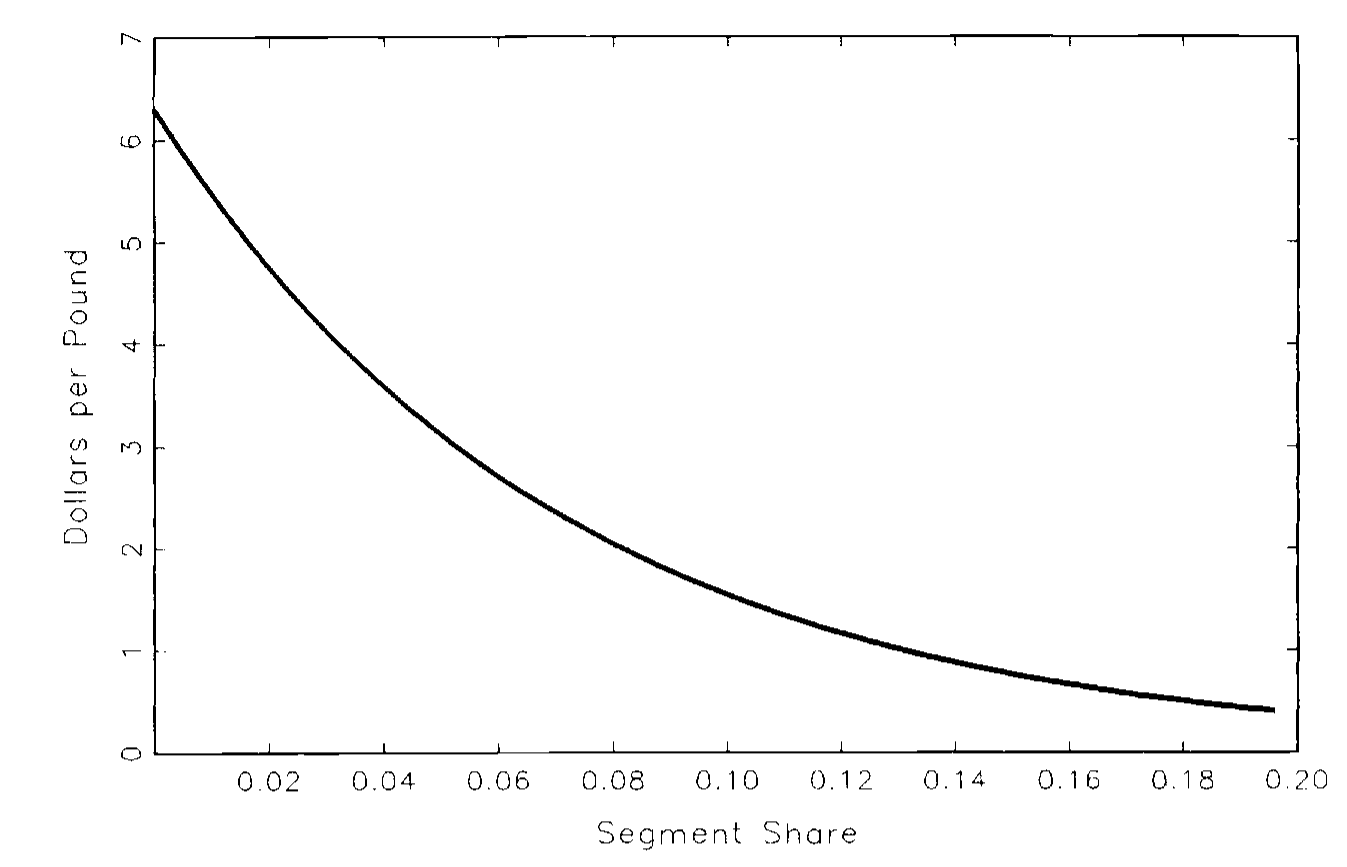
\includegraphics[width=\textwidth]{figures/ch10/hausman_fig5_1.png}
\caption{Method 1: demand at average regressors}
\end{subfigure}\hfill
\begin{subfigure}[t]{0.49\textwidth}
\centering
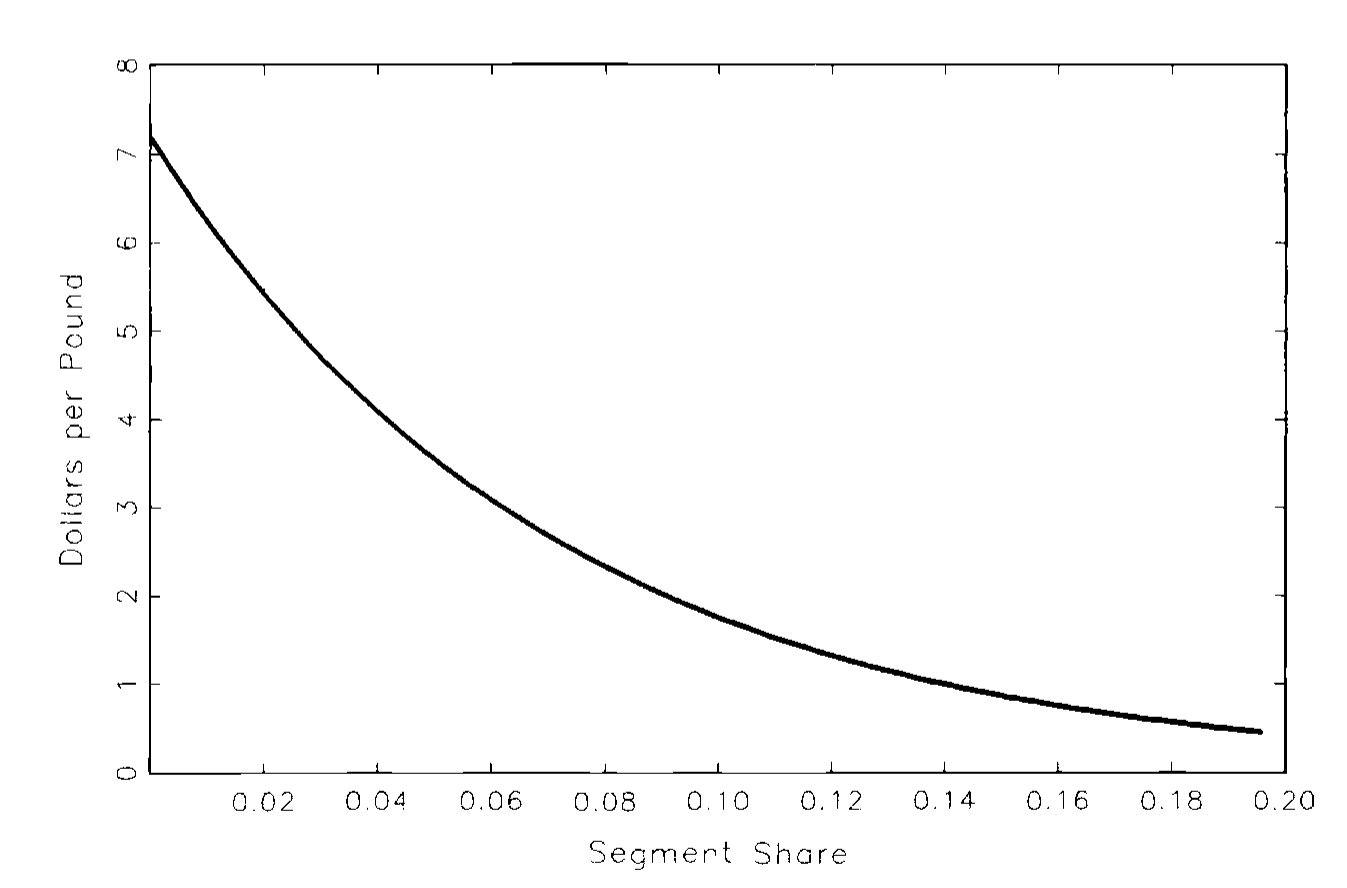
\includegraphics[width=\textwidth]{figures/ch10/hausman_fig5_2.png}
\caption{Method 2: average of 959 city-week curves}
\end{subfigure}
\caption{Estimated AIDS demand curves for Apple-Cinnamon Cheerios. The horizontal axis is ACC's share of
family-segment spending and the vertical axis is the price in dollars per pound. The intercept on the price
axis is the virtual price. Source: Hausman (1997), Figures 5.1 and 5.2.}
\label{fig:10-hausman-aids-curves}
\end{figure}

\casehead{Virtual price}
City virtual prices range from about \$6.00 to about \$7.50. Hausman's best estimate of the aggregate
virtual price is \$7.14, with an asymptotic standard error of \$1.33 (p.~227). The lower end of an
approximate 95 percent confidence interval is \$4.75. Hausman describes it as 35 percent above ACC's average
price of \$3.48 (36.5 percent by our computation).\footnote{A symmetric normal interval would give
$7.14 - 1.96\times 1.33 = \$4.53$ (our computation). Hausman does not say how he computes \$4.75.} The virtual price is about twice the actual price. Hausman finds this reasonable given an own
elasticity of about $-2.2$ (p.~228).

\casehead{Exact consumer surplus}
The exact compensating variation is computed from the expenditure function, by the method of
\citet{HausmanNewey1995} (fn.~24). It is close to the area under the demand curve above \$3.48. The estimate
is \$32,268 per city per week, with an asymptotic standard error of \$3,384 (p.~228). For the United States
it amounts to about \$78.1 million per year, or about \$0.3136 per person per year. Hausman anticipates the
objection that his method yields small elasticities. The same technique gives own-price elasticities for
beer brands between about $-4.0$ and $-6.2$ in \citet{HausmanLeonardZona1994} (fn.~25).

\casehead{A bound robust to extrapolation}
Observed prices never come near the virtual price, so \$7.14 rests on the shape of the estimated curve far
outside the data. Hausman addresses this with a supporting line. If demand is convex, the tangent at the
observed point lies below the curve and meets the price axis below the true intercept. This is the logic of
\cref{prop:10-tangent}. Drawing the tangent to the curves of \cref{fig:10-hausman-aids-curves} at \$3.48
gives lower bounds between \$5.55 and \$5.94, with a standard error of about \$0.15 (p.~228). The bounds lie
about 65 percent above the average price.\footnote{The tangents are drawn in the share-price plane of the
figures. In the quantity-price plane, \cref{prop:10-tangent} with ACC's overall elasticity of $-2.173$ gives
$3.48\bigl(1 + \frac{1}{2.173}\bigr) = \$5.08$ (our computation). Convexity in one plane does not imply
convexity in the other, since the share is proportional to price times quantity.}

\casehead{Two consistency checks}
Two checks of our own relate these numbers to the theory of \cref{sec:10-virtual}. Hausman's pound volumes
and prices imply family-segment spending of about \$1.14 million per city-week, so ACC sells about 20,300
pounds a week in a typical city.\footnote{We compute these figures from Table 5.2 and p.~234. Cheerios sells 93,738
pounds at \$2.644 with a segment share of 0.216, and Honey-Nut sells 47,215 pounds at \$3.605 with a share of
0.150. The two imply segment spending of \$1.147 and \$1.133 million. ACC's volume is
$\frac{0.0619 \times 1.14\text{ million}}{3.48}$.} First, the Paasche rectangle of
\cref{prop:10-index-bounds} is $(7.14 - 3.48)\times 20{,}300 \approx \$74{,}200$. The exact surplus,
\$32,268, is 43 percent of it. A linear Hicksian curve would give exactly half, and a convex curve lies below
the chord, so the share below one half is what convexity predicts. Second, the rectangle is about 1.7 percent
of cereal spending, which matches the index effect Hausman reports below.

\begin{table}[htbp]
\centering
\caption{Welfare effects of Apple-Cinnamon Cheerios}\label{tab:10-hausman-welfare}
\begin{threeparttable}
\begin{tabular}{@{}lll@{}}
\toprule
Quantity & Estimate & Page \\
\midrule
\multicolumn{3}{@{}l}{\textit{Perfect competition (AIDS)}} \\
Virtual price, aggregate & \$7.14 (1.33) & 227 \\
Virtual price, range across cities & \$6.00 to \$7.50 & 227 \\
Lower end of approximate 95\% interval & \$4.75 & 227 \\
Tangent lower bound on virtual price & \$5.55 to \$5.94 (about 0.15) & 228 \\
Consumer surplus per city per week & \$32,268 (3,384) & 228 \\
Consumer surplus, United States, per year & \$78.1 million & 228 \\
Consumer surplus per person per year & \$0.3136 & 228 \\[2pt]
\multicolumn{3}{@{}l}{\textit{Alternative specification}} \\
CES virtual price & infinite & 231 \\
CES consumer surplus & about $3 \times$ AIDS & 231 \\[2pt]
\multicolumn{3}{@{}l}{\textit{Imperfect competition (rivals' prices fixed)}} \\
Loss from higher Cheerios prices, city-week & \$890 + \$3,715 = \$4,605 & 234 \\
Net gain per city-week & \$27,395 (85.6\% of \$32,000) & 234 \\
Net gain, United States, per year & \$66.8 million, \$0.268 per person & 234 \\[2pt]
\multicolumn{3}{@{}l}{\textit{Cereal price index}} \\
Overstatement, perfect competition & about 25\% & 229 \\
Overstatement, imperfect competition & about 20\% & 234 \\
\bottomrule
\end{tabular}
\begin{tablenotes}[flushleft]\footnotesize
\item Notes: Compiled from the text of \citet{Hausman1997}, pp.~227--234. Asymptotic standard errors in
parentheses. The net gain uses a rounded perfect-competition surplus of \$32,000. The index overstatements
refer to the cumulative effect of brands introduced over ten years.
\end{tablenotes}
\end{threeparttable}
\end{table}

\Cref{tab:10-hausman-welfare} collects the welfare results of the paper.

\subsection{Implications for the cereal price index}\label{sec:10-hausman-index}

Hausman translates the surplus into a price-index correction (pp.~228--229). Treating ACC as part of
Honey-Nut Cheerios would show almost no effect, beyond ACC's slightly lower price. Suppose instead, contrary
to fact, that all of ACC's share came from Honey-Nut. With ACC valued at its virtual price before
the introduction, the price index of the two brands falls from about \$4.60 to about \$3.57, or 22 percent. The
family-segment index falls from \$3.10 to \$2.88, or 7.1 percent. The overall cereal index falls by about
0.017, or \$0.052, about 1.7 percent. These figures are share-weighted average prices with ACC valued at
\$7.14 in the base period.\footnote{We approximately reproduce these figures from Table 5.2. The Honey-Nut and
ACC composite is $\frac{15.03 \times 3.605 + 6.19 \times 7.14}{21.22} = \$4.64$ before and
$\frac{15.03 \times 3.605 + 6.19 \times 3.48}{21.22} = \$3.57$ after, a fall of 23 percent. The family index is
\$2.88 with ACC at \$3.48 and \$3.11 with ACC at \$7.14. The small gaps from Hausman's \$4.60, 22 percent and
\$3.10 presumably reflect rounding.}

Hausman then states a rule of thumb. The change in the overall index is approximately ACC's share of cereal
spending, 1.6 percent, times the gap between the virtual and the actual price relative to the actual price.
If the virtual price is twice the actual price, the index change roughly equals the new brand's share. About
25 percent of cereal demand comes from brands introduced in the previous ten years. Suppose these brands sell
at about the same prices as old ones and have virtual prices twice their actual prices. Then the cereal index
that ignores them is too high by about their share, 25 percent (p.~229). Exits reduce the gain, but brands
are withdrawn only when their shares are tiny, so the correction is small and could not be estimated
(fn.~26).

The rule of thumb is the Paasche rectangle of \cref{prop:10-index-bounds}, expressed as a share of spending:
$w_n\bigl(\frac{p_n^V}{p_n} - 1\bigr)$. The proposition shows that this rectangle exceeds the exact gain for
any downward-sloping Hicksian curve. Hausman's own surplus estimate is 43 percent of the rectangle, about
0.75 percent of cereal spending against the 1.7 percent of the rule. Applying the same ratio to his
extrapolation would cut the 25 percent figure to about 11 percent, and the imperfect-competition figure of
20 percent to about 9 percent.\footnote{We compute $0.435 \times 25 = 10.9$ and
$0.435 \times 0.856 \times 25 = 9.3$. The extrapolation also assumes that every new brand of the decade
resembles ACC, a strong assumption that Hausman calls ``perhaps unrealistic'' (p.~229).} The correction
remains large by the standards of price measurement. The main conclusion survives, but the rectangle
overstates the exact effect by a factor of about two.

\subsection{Alternative specifications: attributes, logit and CES}\label{sec:10-hausman-ces}

Section 5.5 of the paper explains why Hausman prefers a flexible product-space system. Attribute models in
the Hotelling, Gorman and Lancaster tradition describe a product by its characteristics and predict demand
for new products from them (\citealp[fn.~27]{Hausman1997}, citing \citealp{PakesBerryLevinsohn1993}).
Hausman argues that ACC cannot be described by attributes, ``perhaps the volume of apples and cinnamon''
(p.~229). He adds that no metric measures how close attributes are and no aggregator combines them. The
right measure of closeness, in his view, is the cross-price elasticity. His experience with probit models of
French champagne makes the point: ``the bubble content could never be made to come in significant'' (fn.~28,
on the models of \citealp{HausmanWise1978}). The logit model has the independence of irrelevant alternatives
(IIA) property, which ``typically leads to a vast overestimate'' of the surplus from a new good (p.~230). The
nested logit still has IIA within each nest. \Cref{sec:10-charspace} takes up the case for characteristics
models.

\casehead{CES demand}
Hausman compares his estimates with the constant elasticity of substitution (CES) model of
\citet{DixitStiglitz1977}, which treats all goods symmetrically. Utility is
\begin{equation}\label{eq:10-h-ces-u}
  U(x_1,\dots,x_n) = \Bigl(\sum_{i=1}^{n}x_i^{\rho}\Bigr)^{\frac{1}{\rho}}, \qquad 0 < \rho < 1
\end{equation}
(Hausman's eq.~9). Write $\eta = \frac{1}{1-\rho}$ for the elasticity of substitution, so that
$1 - \eta = -\frac{\rho}{1-\rho}$. Maximizing \eqref{eq:10-h-ces-u} subject to $\sum_i p_ix_i = y$ gives the
Marshallian demand implied by \eqref{eq:10-ces-share} with equal taste parameters,
\begin{equation}\label{eq:10-h-ces-demand}
  x_k = \frac{y\,p_k^{-\eta}}{\sum_{i=1}^{n}p_i^{1-\eta}}.
\end{equation}
Hausman's eq.~10 writes the compensated version. The unit expenditure function is
$c(p) = \bigl(\sum_ip_i^{1-\eta}\bigr)^{\frac{1}{1-\eta}}$, and Hicksian demand is
$x_k = U\bigl(\frac{p_k}{c(p)}\bigr)^{-\eta} = U\,p_k^{-\eta}\bigl(\sum_ip_i^{1-\eta}\bigr)^{-\frac{\eta}{\eta-1}}$.
Since $\frac{\eta}{\eta-1} = \frac{1}{\rho}$, this equals
$\bigl[\frac{\sum_ix_i^{\rho}}{\sum_ip_i^{-\frac{\rho}{1-\rho}}}\bigr]^{\frac{1}{\rho}}p_k^{-\frac{1}{1-\rho}}$, which
is eq.~10 without its error term. Taking logs of \eqref{eq:10-h-ces-demand},
$\ln x_k = \ln y - \eta\ln p_k - \ln\sum_ip_i^{1-\eta}$. Differentiating with respect to $\ln p_j$ and writing
$w_j = \frac{p_j^{1-\eta}}{\sum_ip_i^{1-\eta}}$ for the spending share,
\begin{equation}\label{eq:10-h-ces-elast}
  \varepsilon_{kj} = -\eta\,\indic\{k = j\} + (\eta - 1)w_j.
\end{equation}
Every product has the same cross elasticity with respect to $p_j$, which is Hausman's eq.~11. Own elasticities
depend only on the share and on $\eta$, ``a property without any empirical foundation'' (p.~231). Demand
\eqref{eq:10-h-ces-demand} is positive at every finite price, so the CES virtual price is infinite.

\casehead{Estimates}
Hausman estimates the CES model by nonlinear two-stage least squares (p.~231). He reports
$\hat\rho = 0.580$ with an asymptotic standard error of 0.00001 and an elasticity of substitution of 2.13.
The two printed numbers are inconsistent, since $\frac{1}{1 - 0.580} = 2.38$, while 2.13 corresponds to
$\rho = 0.53$. We cannot tell which is the typographical error. \Cref{fig:10-hausman-ces} shows the
estimated CES curve. It rises steeply as the share approaches zero and never meets the price axis. The
consumer surplus, the area under this curve above the price, is ``about three times as high'' as the AIDS
estimate of \$78.1 million a year (p.~231).

\begin{figure}[htbp]
\centering
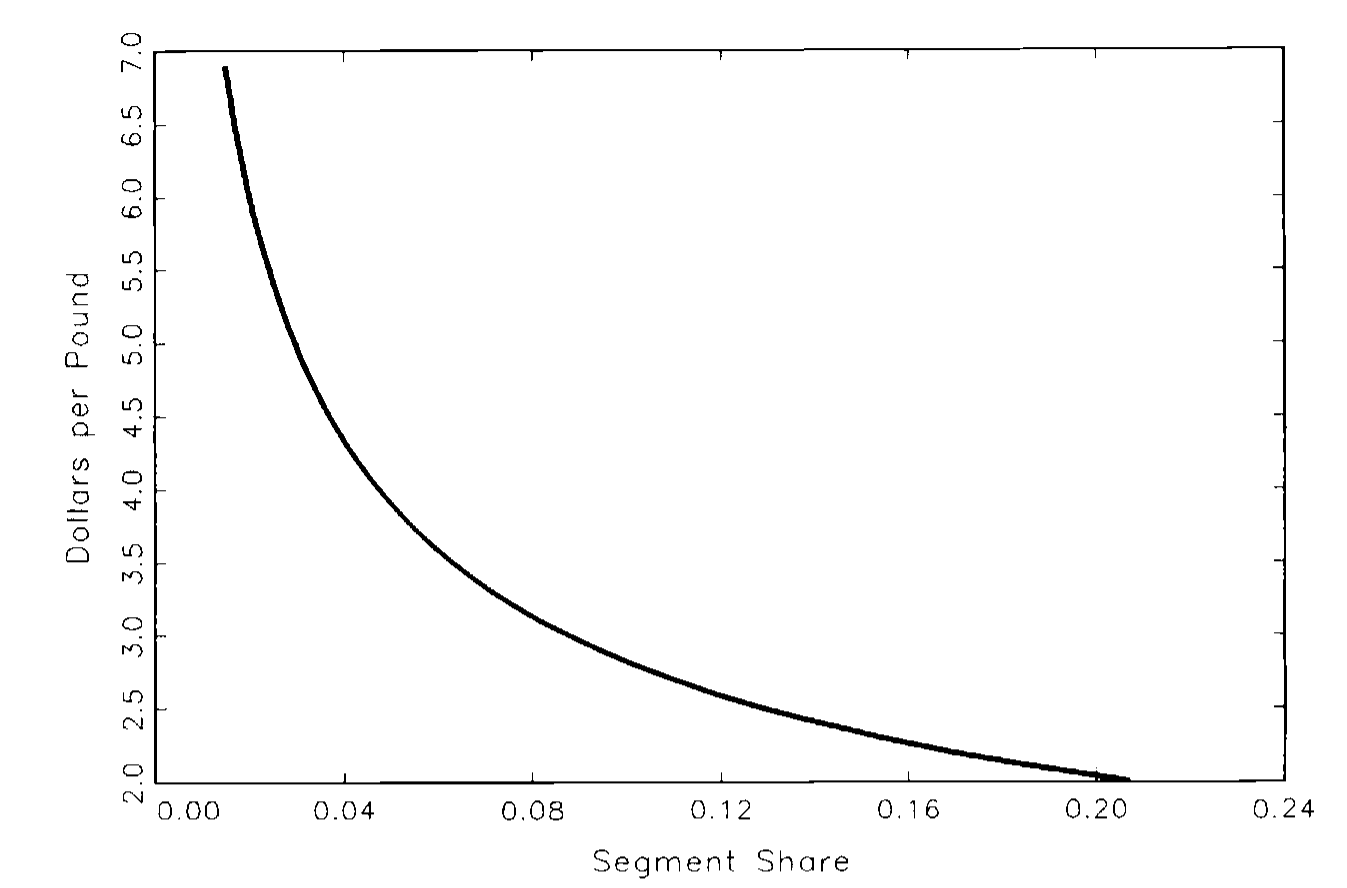
\includegraphics[width=0.75\textwidth]{figures/ch10/hausman_fig5_3.png}
\caption{Estimated CES demand curve for family-segment brands. The horizontal axis is the segment share and
the vertical axis the price in dollars per pound. The curve never meets the price axis, so the virtual price
is infinite. Source: Hausman (1997), Figure 5.3.}
\label{fig:10-hausman-ces}
\end{figure}

The comparison teaches a lesson about functional form. At ACC's segment share of 0.0619,
\eqref{eq:10-h-ces-elast} gives an own elasticity of $-2.13 + 1.13 \times 0.0619 = -2.06$ with $\eta = 2.13$.
This is close to the AIDS value of $-2.12$. The two systems thus give similar own elasticities at the data and diverge
mainly in the extrapolation to zero quantity. The share-only CES formula of \cref{cor:10-ces-newgood} implies,
as computed in \cref{sec:10-feenstra}, that ACC lowers the cost of living of the family segment by 5.5 percent.
The equivalent variation is then 5.5 percent of family-segment spending, about \$63,000 per city-week, and the
compensating variation is 5.8 percent. Both are about twice the AIDS surplus. With $\eta = 2.38$ the fall in the
cost of living is 4.5 percent.\footnote{These are our computations,
using segment spending of \$1.14 million per city-week. Hausman's ``three times'' integrates his estimated
CES curve, so the two comparisons are not identical. Both put the CES valuation at a multiple of the AIDS
valuation.} In the CES and the logit, the value of variety is built into the functional form. The AIDS
lets the data choose a finite virtual price, at the cost of relying on the curvature of the estimated curve.

\subsection{Imperfect competition}\label{sec:10-hausman-imperfect}

The classical analysis assumes that other prices stay at marginal cost when the new good arrives. Hausman
notes that most new brands come from multiproduct firms (p.~231). When General Mills raises the price of
Cheerios, some of the lost buyers now switch to ACC instead of a rival brand. The firm keeps that demand, so
the introduction lets it raise the prices of its existing brands. This effect lowers the consumer gain.

\casehead{Pricing equations}
\Cref{sec:10-multiproduct} derives Hausman's pricing equations in the notation of this chapter. A single-product
firm under Nash-Bertrand pricing sets $\frac{p_1 - mc_1}{p_1} = -\frac{1}{\varepsilon_{11}}$ (Hausman's eq.~12). A
firm selling brands $k = 1,\dots,K$ satisfies the elasticity form \eqref{eq:10-foc-elast} of its first-order
conditions (his eq.~13), with $w_k$ the revenue share of brand $k$ in the firm's sales. In matrix form these are
\eqref{eq:10-foc-matrix}, $w + E^\top m = 0$ and $m = -(E^\top)^{-1}w$ (his eqs.~14 and 15), where
$m_k = \frac{p_k - mc_k}{p_k}w_k$. Dividing each $m_k$ by $w_k$ gives the Lerner index of brand $k$.

\casehead{The calculation}
Hausman solves \eqref{eq:10-foc-matrix} for the General Mills family brands with ACC and without it. He
holds marginal costs constant and assumes that ``other firms, such as Kellogg, will not change their prices
in response to the introduction'' (p.~234). He claims that the resulting price changes are ``a lower bound
on expected price changes, absent new entry by competitors'' (p.~233). \Cref{tab:10-hausman-margins}
reproduces the results.

\begin{table}[htbp]
\centering
\caption{Nash-Bertrand price-cost margins of the General Mills family brands}\label{tab:10-hausman-margins}
\begin{threeparttable}
\begin{tabular}{@{}lcc@{}}
\toprule
 & Cheerios & Honey-Nut Cheerios \\
\midrule
Price-cost margin & 0.5268 & 0.5203 \\
Price-cost margin without Apple-Cinnamon Cheerios & 0.5251 & 0.5096 \\
Price-cost margin if brand were independent & 0.5193 & 0.5050 \\
\bottomrule
\end{tabular}
\begin{tablenotes}[flushleft]\footnotesize
\item Notes: Reproduced in full from \citet[Table 5.7]{Hausman1997}. Margins are Lerner indexes
$\frac{p - mc}{p}$ from \eqref{eq:10-foc-matrix}. The last row is $-\frac{1}{\varepsilon_{jj}}$ with the overall
own elasticities of Table 5.6: $\frac{1}{1.92572} = 0.5193$ and $\frac{1}{1.98037} = 0.5050$. Rivals' prices
and marginal costs are held fixed.
\end{tablenotes}
\end{threeparttable}
\end{table}

The margins rise when ACC joins the line, and they exceed the single-product margins of the last row. With
constant marginal cost, \eqref{eq:10-price-ratio} converts the margins into the ratio
$r_k = \frac{p_k^{\text{with}}}{p_k^{\text{without}}}$ of the prices with and without ACC. The 1992 prices of
Table 5.2 are observed with ACC on the market. The price without ACC is therefore $\frac{p_k^{\text{with}}}{r_k}$,
and the price increase is $p_k^{\text{with}} - \frac{p_k^{\text{with}}}{r_k} = p_k^{\text{with}}\bigl(1 - \frac{1}{r_k}\bigr)$.
For Cheerios, the ratio is $\frac{1 - 0.5251}{1 - 0.5268} = \frac{0.4749}{0.4732} = 1.0036$. At the 1992 price of \$2.644
the increase is $2.644 \times \bigl(1 - \frac{0.4732}{0.4749}\bigr) = \$0.0095$. For Honey-Nut, the ratio is
$\frac{0.4904}{0.4797} = 1.0223$, and at \$3.605 the increase is
$3.605 \times \bigl(1 - \frac{0.4797}{0.4904}\bigr) = \$0.0787$. Both are the figures Hausman
reports.\footnote{This is our computation. The implied prices without ACC are \$2.635 and \$3.526. The paper
also reports markup increases of 0.32 and 3.0 percent. The first is the ratio of the Cheerios
margins, $\frac{0.5268}{0.5251} = 1.0032$. The same ratio for Honey-Nut is 1.021.} The larger effect on
Honey-Nut is expected, since ACC is a closer substitute for Honey-Nut than for Cheerios.

\casehead{Welfare}
Average weekly sales per city are 93,738 pounds of Cheerios and 47,215 pounds of Honey-Nut (p.~234). To first
order, the price increases cost consumers $0.0095 \times 93{,}738 = \$890$ and $0.0787 \times 47{,}215 =
\$3{,}715$ per city-week, a total of \$4,605. Hausman compares this loss with ``the \$32,000--44,000 consumer's
surplus estimates''. The net gain is $\$32{,}000 - \$4{,}605 = \$27{,}395$, which is 85.6 percent of the
Hicksian gain (p.~234). Per year the gain is \$66.8 million, or \$0.268 per person. The overstatement of the
cereal CPI falls from about 25 percent to about 20 percent. Hausman notes that his data begin after ACC's
launch, so he cannot compare prices before and after it directly. He leaves such a study for future research
(p.~234).

\casehead{What the calculation holds fixed}
Reproducing Table 5.7 shows exactly what the counterfactual changes. The ``without'' row deletes ACC's row and
column from the elasticity matrix and ACC's entry from the share vector. It keeps the shares and elasticities
of Cheerios and Honey-Nut at their values with ACC present.\footnote{This is our computation. We solve
\eqref{eq:10-foc-matrix} with the mean revenue shares of Table 5.5 and the Cheerios block of Table 5.6. The
solution reproduces the four margins in the first two rows of Table 5.7 to four decimals.} In the language of
\cref{sec:10-imperfect}, the calculation captures only the new term that ACC adds to the first-order
conditions. Before the launch, Cheerios and Honey-Nut had larger shares. The fall in their shares is the
source of the two offsetting effects that \citet{Bresnahan1997} stresses, and the calculation omits it.
Rivals' prices are held fixed as well. \Cref{sec:10-bresnahan-competition}
returns to both points.

\begin{remark}[The orientation of the elasticity matrix in Table 5.7]\label{rem:10-margins-orientation}
Table 5.7 is reproduced exactly when Table 5.6 is read with rows as quantities, the layout that
\eqref{eq:10-foc-matrix} requires. \Cref{rem:10-orientation} shows that Table 5.6 is printed with rows as
prices. The two facts together imply that the margins were computed with $\varepsilon_{jk}$ where
\eqref{eq:10-foc-elast} requires $\varepsilon_{kj}$. Recomputing with the layout implied by
\cref{rem:10-orientation}, and changing nothing else, gives margins with ACC of 0.5250 (Cheerios), 0.5402
(Honey-Nut) and 0.5251 (ACC), and without ACC of 0.5215 and 0.5169. Relative to the prices without ACC,
the implied increases are 0.7 percent for Cheerios and 5.1 percent for Honey-Nut. In dollars,
$p_k^{\text{with}}\bigl(1 - \frac{1}{r_k}\bigr)$ gives \$0.0192 and \$0.1739 per pound. The first-order loss becomes
\$10,004 per city-week, and the net gain 68.7 percent of \$32,000.\footnote{We computed these values with
\texttt{figures/ch10/src/hausman\_reproduction.py}. With the printed layout, the same program gives ACC's own
margin as 0.6201, a value the paper does not report.} The direction is intuitive. In Honey-Nut's first-order
condition the relevant cross effect is the response of ACC's volume to Honey-Nut's price, which is 0.21. The
printed layout uses instead the response of Honey-Nut's volume to ACC's price, which is 0.08. We offer this
as a reproduction exercise, since the paper itself does not confirm our reading of Table 5.6. It shows that
the imperfect-competition adjustment is sensitive to a detail that papers rarely state, the layout of the
elasticity matrix.
\end{remark}

\subsection{Robustness}\label{sec:10-hausman-robustness}

The paper reports several robustness checks, mostly in footnotes. Monthly data give elasticities similar to
the weekly estimates, with less precision (fn.~21). The segmentation is not rejected by specification tests
(fn.~22). A middle level that does not impose exact two-stage budgeting gives similar results (fn.~17). The
choice between exact and Stone segment indexes ``does not typically have much influence'' (p.~218). The two
aggregation methods for the virtual price give intercepts of about \$6.30 and \$7.20. The tangent bound
limits the role of extrapolation, and the CES comparison shows the direction of functional-form bias.

Other checks are missing. The paper reports no estimates with alternative instruments, no first-stage
statistics and no outcome of the overidentification tests that fn.~20 mentions. It reports no test of the
independence of demand shocks across cities, the assumption on which identification rests. Table 5.7 has no
standard errors, and the imperfect-competition calculation fixes rivals' prices without a sensitivity
analysis. \Cref{sec:10-bresnahan} shows why the first omission matters most.

\subsection{Interpretation, critiques and contribution}\label{sec:10-hausman-assessment}

Taken at face value, the estimates say that consumers value even a close variant of existing brands
highly. ACC's demand curve is steep relative to its volume. The virtual price is twice the actual price, and
the surplus is about 46 percent of ACC's revenue.\footnote{By our computation, the surplus of \$32,268 compares with revenue of
about \$70,600 per city-week.} If incremental brands are typical, official price indexes for branded
consumer goods understate real income growth.

Four lines of critique follow from the theory of this chapter. First, the estimates rest on instruments that
fail if national demand shocks move prices in all cities at once (\cref{sec:10-bresnahan-iv}). Second, the
virtual price is an extrapolation, and the surplus depends on the curvature of the AIDS curve beyond the data
(\cref{sec:10-functional}). The tangent bound helps, but it requires convexity. Third, the
imperfect-competition adjustment holds rivals' prices fixed and keeps post-launch shares in the
counterfactual (\cref{sec:10-bresnahan-competition}). Fourth, the price-index extrapolation uses the Paasche
rectangle, which exceeds the exact gain, and assumes that all new brands resemble ACC
(\cref{sec:10-hausman-index}).

The paper made several contributions. It showed how to compute the exact value of a new brand from scanner
data. It combined the virtual price of \citet{Hicks1940} and \citet{Rothbarth1941} with the exact surplus
methods of \citet{Hausman1981} and \citet{HausmanNewey1995}. Together with \citet{HausmanLeonardZona1994}, it
made multistage budgeting with an unrestricted bottom level a practical tool. The two papers also introduced
prices in other markets as instruments, now a standard device in demand estimation \citep{Nevo2001}. Finally, it raised the question of how market power changes the value of
a new good. The answer it gave was incomplete, as the next section explains, but the question has shaped the
literature since, including the work of \citet{Petrin2002} in \cref{sec:10-petrin}.

\section{Bresnahan's Comment: instruments and competition}\label{sec:10-bresnahan}

\citet{Bresnahan1997} accepts the importance of the question and much of the specification. He disputes
the instruments and the treatment of competition. His comment opens with a statistic: \emph{Brandweek}
counted over 22,000 new-product introductions in 1994 (p.~237). Theory cannot say whether markets supply too
many or too few varieties (fn.~1, quoting \citealp{EatonLipsey1989}, as discussed in \cref{sec:10-private-social}).
So the value of incremental variety is an empirical question, and Hausman's paper is an important attempt to
answer it. This section develops Bresnahan's four points in turn, with the formal
analysis that he sketches in his appendix.

\subsection{Why a steep single-product demand curve means large value}\label{sec:10-bresnahan-dd}

Bresnahan frames the issue with \cref{fig:10-dd-DD}. The steep curve $DD$ is market demand. The flatter
curve $dd$ is the demand for one product when the prices of its substitutes are held fixed. The flat line
$dd(-\infty)$ is the demand for a product that is a perfect substitute for others. Introducing a product at
price $P_1$ creates the shaded triangle between $dd$, the price axis and the line at $P_1$. Before the
introduction the product was in effect priced at $P_0$, where $dd$ meets the price axis. This is the virtual
price of \cref{sec:10-virtual}.

\begin{figure}[htbp]
\centering
\begin{tikzpicture}[scale=1.0, >=Stealth]
  \draw[->] (0,0) -- (7.4,0) node[below] {$Q$};
  \draw[->] (0,0) -- (0,5.4) node[left] {$P$};
  \fill[black!70] (0,4) -- (0,2.9) -- (2.383,2.9) -- cycle;
  \draw[thick] (1.6,5.0) -- (5.3,0.17) node[right] {$DD$};
  \node at (1.95,5.15) {$DD$};
  \draw[thick] (0,4) -- (6.8,0.862) node[right] {$dd$};
  \node at (0.95,3.8) {$dd$};
  \draw[thick] (0,2.311) -- (7.0,2.311) node[right] {$dd(-\infty)$};
  \draw[dashed] (2.383,2.9) -- (2.383,0);
  \node[left] at (0,4) {$P_0$};
  \node[left] at (0,2.9) {$P_1$};
  \node[below] at (2.383,0) {$q_1$};
  \fill (3.659,2.311) circle (1.5pt);
\end{tikzpicture}
\caption{Consumers' gain from a new product. $DD$ is market demand, $dd$ the demand for a single product at
fixed prices of its substitutes, and $dd(-\infty)$ the demand for a perfect substitute. Selling the product
at $P_1$ instead of its choke price $P_0$ yields the shaded surplus. The steeper is $dd$, the larger the
triangle for a given volume $q_1$. Source: redrawn after Bresnahan (1997), Figure 5C.1.}
\label{fig:10-dd-DD}
\end{figure}

The area of the triangle makes the point precise. Let $dd$ be linear with slope $-s$ in the $(Q, P)$ plane,
where $s > 0$ measures its steepness. A product sold at $P_1$ in volume $q_1$ then has choke price
$P_0 = P_1 + s\,q_1$. Its surplus is
\begin{equation}\label{eq:10-b-triangle}
  CS = \frac{1}{2}(P_0 - P_1)\,q_1 = \frac{s}{2}\,q_1^2.
\end{equation}
For a given volume the surplus is proportional to the steepness $s$, and it vanishes as $dd$ flattens to
$dd(-\infty)$. Treating new goods as perfect substitutes, as hedonic quality adjustment implicitly does,
therefore sets their value to zero. Linking a new good into a price index late treats it as irrelevant in
its early life, and the later the link, the larger the error (p.~238). Both practices understate the value
of new goods. Bresnahan notes a converse in fn.~2. If a new good is a perfect substitute, the law of one price
holds, and late linking does no harm.

Hausman's finding is a steep $dd$ for ACC. \citet{Trajtenberg1989}, whose work \cref{sec:10-trajtenberg}
studies, conjectured that the distance of a new good from existing products in characteristics space governs
the slope of $dd$ (fn.~3). The same steepness has a second implication, developed in
\cref{sec:10-bresnahan-competition}. A product with a steep $dd$ that is sold by one firm carries market
power. Consumer surplus and imperfect competition are therefore linked from the start.

\subsection{Is the large surplus an artifact of the specification?}\label{sec:10-bresnahan-spec}

Bresnahan concludes that it is not (pp.~239--240). A skeptic might suspect that existing Cheerios products
already satisfy ``pretty much any palate''. Hausman's large surplus must then come from finding poor
substitutability between ACC and the other family brands. Within the segment, the AIDS imposes almost no
structure on own and cross elasticities, so the finding comes from the data. The more restrictive CES gives
an even larger surplus (fn.~4).

The segment structure is an assumption, which Bresnahan does not find worrying. It is not interesting to
ask whether two children's cereals substitute more closely than a children's cereal and Special K. The
segments come from marketing research based on richer data, including consumer microdata. Bresnahan adds a
caution for other industries (fn.~5). In automobiles, brand names and country reputations compete with size
classes as principles of grouping, and in many consumer goods private labels form a further group. The
simple structure of cereal is the exception.

\subsection{Instruments and national demand shocks}\label{sec:10-bresnahan-iv}

The treatment of price endogeneity is the other place where the conclusion might have been ``accidentally
assumed'' (p.~240). Hausman's identifying assumption is that the shocks $\omega_{jnt}$ in
\eqref{eq:10-h-price} are independent across cities. This rules out every national shock to the demand for
one brand relative to another. In Bresnahan's words, ``there can be no successful nationwide advertising
campaigns which shift the demand for individual brands or products'' (p.~241). There can be no national
fads and no slow national acceptance of new brands. Including advertising in the demand system does not
solve the problem, because the econometrician does not observe which campaigns succeed (fn.~6).

Hausman's fallback is that prices are predetermined. Economically, this requires that national demand shocks
cannot be foreseen when prices are set. Bresnahan finds this unlikely for shocks such as advertising
campaigns, which manufacturers plan and communicate to retailers in advance. If national shocks exist and
are reflected in prices, and if supply slopes up, prices in other cities are correlated with the demand
error. Supply slopes up in the one-week run because inventories cannot adjust or because of market power
(fn.~7). Hausman's own pricing equations imply an upward-sloping supply relation.

\casehead{The model}
We formalize the argument with one product, following Bresnahan's simple case: linear demand, single-product
Bertrand pricing and constant marginal cost (p.~241). In city $n$ and week $t$,
\begin{equation}\label{eq:10-b-demand}
  q_{nt} = d_n - b\,p_{nt} + \xi_{nt}, \qquad b > 0,
\end{equation}
where $d_n$ is a city effect. Marginal cost is $c_{nt} = c_n + k_t + v_{nt}$. The national cost component
$k_t$ has variance $\sigma_k^2$, and the local component $v_{nt}$ has variance $\sigma_v^2$. The demand error
has a national and a local part, $\xi_{nt} = \chi_t + e_{nt}$. Each part splits into a component that is
anticipated when prices are set and one that is not: $\chi_t = \chi^a_t + \chi^u_t$ and
$e_{nt} = e^a_{nt} + e^u_{nt}$, with variances $\sigma_{\chi a}^2$, $\sigma_{\chi u}^2$, $\sigma_{ea}^2$ and
$\sigma_{eu}^2$. All components have mean zero and are mutually independent. Local components are
independent across cities. City effects are removed by the within transformation, so we treat $d_n$ and
$c_n$ as known.

\casehead{Pricing}
The firm sets $p_{nt}$ to maximize expected profit $\E[(p - c_{nt})(d_n - bp + \xi_{nt})\mid\mathcal{I}_{nt}]$,
where the information set $\mathcal{I}_{nt}$ contains costs and the anticipated shocks. The first-order
condition is
\begin{equation*}
  d_n - 2b\,p_{nt} + \E[\xi_{nt}\mid\mathcal{I}_{nt}] + b\,c_{nt} = 0.
\end{equation*}
Solving for the price,
\begin{equation}\label{eq:10-b-price}
  p_{nt} = \frac{1}{2}\Bigl(c_{nt} + \frac{d_n + \chi^a_t + e^a_{nt}}{b}\Bigr).
\end{equation}
Equivalently $p_{nt} = c_{nt} + \frac{\E[q_{nt}\mid\mathcal{I}_{nt}]}{b}$, the expected-quantity version of
Bresnahan's supply relation $P = Q(-\gamma_{jj})^{-1} + c$. With fully anticipated shocks this is his model,
and with no anticipated shocks prices are predetermined in Hausman's sense.

\casehead{Estimators}
The Hausman estimator of $-b$ is the instrumental-variables (IV) estimator that uses $p_{\ell t}$, the
price in another city $\ell\neq n$, as the instrument for $p_{nt}$. Averaging over several other cities, as
our simulation does, has the same probability limit. Ordinary least squares (OLS) regresses $q_{nt}$ on
$p_{nt}$. Both use within-city deviations.

\begin{proposition}[Hausman instruments with national demand shocks]\label{prop:10-hausman-iv-bias}
In the model given by \eqref{eq:10-b-demand} and \eqref{eq:10-b-price}, define
\begin{equation*}
  \lambda = \frac{\sigma_{\chi a}^2}{b^2\sigma_k^2 + \sigma_{\chi a}^2}, \qquad
  \lambda_{OLS} = \frac{\sigma_{\chi a}^2 + \sigma_{ea}^2}{b^2(\sigma_k^2 + \sigma_v^2) + \sigma_{\chi a}^2 + \sigma_{ea}^2}.
\end{equation*}
Then, as the number of weeks grows,
\begin{equation}\label{eq:10-b-plim}
  \plim\hat b_{IV} = b(1 - 2\lambda), \qquad \plim\hat b_{OLS} = b(1 - 2\lambda_{OLS}).
\end{equation}
Consequently, the following hold.
\begin{enumerate}[label=(\alph*)]
\item The IV estimator is consistent if and only if there are no anticipated national demand shocks,
$\sigma_{\chi a}^2 = 0$. Local shocks, anticipated or not, cause no bias.
\item If $\sigma_{\chi a}^2 > 0$, the estimated demand curve is too steep. If $\sigma_{\chi a}^2 > b^2\sigma_k^2$,
the estimated slope has the wrong sign.
\item Let $\lambda < \frac{1}{2}$, and take linear demand through the observed point $(p, q)$. The implied consumer surplus
$\frac{q^2}{2\hat b}$ and the implied gap $\frac{q}{\hat b}$ between the virtual and the actual price are
both overstated by the factor $\frac{1}{1 - 2\lambda}$.
\item The IV estimator is less biased than OLS if and only if $\lambda < \lambda_{OLS}$.
\end{enumerate}
\end{proposition}

\begin{proof}
Work with within-city deviations, so that $d_n$ and $c_n$ drop out. From \eqref{eq:10-b-price}, the deviation
of the price is
\begin{equation*}
  \tilde p_{nt} = \frac{1}{2}\Bigl(k_t + v_{nt} + \frac{\chi^a_t + e^a_{nt}}{b}\Bigr).
\end{equation*}
Substituting into \eqref{eq:10-b-demand}, the IV and OLS estimators of the coefficient $-b$ converge to
\begin{equation*}
  -b + \frac{\Cov(\tilde p_{\ell t},\xi_{nt})}{\Cov(\tilde p_{\ell t},\tilde p_{nt})}
  \qquad\text{and}\qquad
  -b + \frac{\Cov(\tilde p_{nt},\xi_{nt})}{\Var(\tilde p_{nt})}.
\end{equation*}
For the IV estimator take $\ell\neq n$. The price in city $\ell$ shares only the national components $k_t$ and
$\chi^a_t$ with city $n$. Of these, only $\chi^a_t$ is correlated with $\xi_{nt}$. Hence
\begin{equation*}
  \Cov(\tilde p_{\ell t},\xi_{nt}) = \frac{1}{2b}\Cov(\chi^a_t,\chi_t) = \frac{\sigma_{\chi a}^2}{2b},
\end{equation*}
\begin{equation*}
  \Cov(\tilde p_{\ell t},\tilde p_{nt}) = \frac{1}{4}\Bigl(\sigma_k^2 + \frac{\sigma_{\chi a}^2}{b^2}\Bigr)
  = \frac{b^2\sigma_k^2 + \sigma_{\chi a}^2}{4b^2}.
\end{equation*}
The ratio of the two is
\begin{equation*}
  \frac{\sigma_{\chi a}^2}{2b}\cdot\frac{4b^2}{b^2\sigma_k^2 + \sigma_{\chi a}^2} = 2b\lambda.
\end{equation*}
So the IV estimate of $-b$ converges to $-b + 2b\lambda$, and $\plim\hat b_{IV} = b - 2b\lambda = b(1 - 2\lambda)$.
For OLS the same steps apply with all anticipated components:
\begin{equation*}
  \Cov(\tilde p_{nt},\xi_{nt}) = \frac{\sigma_{\chi a}^2 + \sigma_{ea}^2}{2b}, \qquad
  \Var(\tilde p_{nt}) = \frac{b^2(\sigma_k^2 + \sigma_v^2) + \sigma_{\chi a}^2 + \sigma_{ea}^2}{4b^2},
\end{equation*}
and the ratio is $2b\lambda_{OLS}$, which gives $\plim\hat b_{OLS} = b(1 - 2\lambda_{OLS})$.

Part (a) follows because $\lambda = 0$ if and only if $\sigma_{\chi a}^2 = 0$, and $\lambda$ does not depend
on $\sigma_{ea}^2$ or $\sigma_{eu}^2$. For part (b), $\lambda > 0$ gives $\plim\hat b_{IV} < b$, and
$1 - 2\lambda < 0$ if and only if $\lambda > \frac{1}{2}$, which is equivalent to
$\sigma_{\chi a}^2 > b^2\sigma_k^2$. For part (c), linear demand through $(p, q)$ with slope $-\hat b$ meets
the price axis at $p + \frac{q}{\hat b}$, and the triangle above $p$ has area $\frac{q^2}{2\hat b}$. Both are
proportional to $\frac{1}{\hat b}$, so their ratios to the true values converge to
$\frac{b}{\plim\hat b_{IV}} = \frac{1}{1 - 2\lambda}$. Part (d) compares the two biases $2b\lambda$ and
$2b\lambda_{OLS}$.
\end{proof}

The weight $\lambda$ has a direct interpretation. The common price component shared by all cities is
$\frac{1}{2}(k_t + \frac{\chi^a_t}{b})$. Its variance is $\frac{1}{4}(\sigma_k^2 + \frac{\sigma_{\chi a}^2}{b^2})$,
and $\lambda$ is the share of that variance due to national demand shocks. The proposition thus says that
the Hausman estimator is a weighted average of the demand slope and the supply slope. With weight
$1 - \lambda$ the common price variation traces out demand, as Hausman assumes. With weight $\lambda$ it
traces out the supply relation $q = b(p - c)$, whose slope is $+b$. This is Bresnahan's remark that with
national demand shocks the estimator ``is like doing ordinary least squares on a supply and demand system''
(p.~242). \Cref{sec:05-bresnahan-critique} derives the same weight in \eqref{eq:05-iv-bias-scalar}. Our version adds the
distinction between anticipated and unanticipated shocks, the OLS comparison and the welfare consequences.

The welfare consequence is large even for modest violations. Suppose anticipated national demand shocks
account for one quarter of the common price variation, so $\lambda = 0.25$. Then the estimated slope is half
the true slope and the surplus is overstated by a factor of two. A share of 10 percent overstates the surplus
by 25 percent. Part (c) is stated for linear demand. For the convex AIDS curves of
\cref{fig:10-hausman-aids-curves} the mapping is only approximate. A curve that is too steep at the data still
implies too large a surplus.

Part (a) also clarifies the debate about predetermined prices. If no national shock is anticipated, both
estimators are consistent when local shocks are unanticipated as well. IV then adds nothing, as Hausman's
second interpretation says. Bresnahan's objection is that the national shocks most likely to matter, such as
advertising campaigns and promotions, are planned in advance. Planned shocks are precisely the anticipated
component that enters $\lambda$. Neither the data nor the paper distinguish the two cases.

\casehead{Many products}
Bresnahan's appendix treats $J$ products. Write demand as $q_{nt} = d + A\,p_{nt} + \xi_{nt}$, with
$a_{jk} = \frac{\partial q_j}{\partial p_k}$ (his $\gamma$), and single-product Bertrand pricing as
$p_{nt} = c_{nt} + D^{-1}q_{nt}$ with $D = \diag(-a_{11},\dots,-a_{JJ})$. Multiplying the pricing equation by
$D$ and substituting demand gives $Dp_{nt} = Dc_{nt} + d + Ap_{nt} + \xi_{nt}$, so the prices solve
$p_{nt} = (D - A)^{-1}(d + Dc_{nt} + \xi_{nt})$. Bresnahan states that the sign and size of the bias are
governed by $\Sigma^{\mathrm{nat}}[\diag(-\gamma) - \gamma]^{-1}$, where $\Sigma^{\mathrm{nat}}$ is the
covariance matrix of the national demand shocks. This is the covariance between other-city prices and demand
errors. For two products whose national shocks have correlation $\varrho$, his appendix reports that the
on-diagonal bias has the sign of $-2\gamma_{22} + \varrho\gamma_{12}$ and the off-diagonal bias the sign of
$\gamma_{12} - 2\varrho\gamma_{11}$ (p.~247). At $\varrho = 0$ both signs are positive when the goods are
substitutes ($\gamma_{12} > 0$). Bresnahan reads them as a bias of own-price coefficients toward zero and of
cross-price coefficients away from zero. These are signs of the covariance between instruments and demand
errors. With several endogenous prices the bias also involves the inverse of the instrument-price
covariance, so the signs need not carry over. Bresnahan notes that the cross-price claim depends on the
correlation of national shocks across products (fn.~9). \Cref{prop:05-iv-bias} gives the exact probability
limit, $\plim\hat A = (I - \Lambda)A + \Lambda D$ with
$\Lambda = \Sigma^{\mathrm{nat}}(D\Sigma_cD + \Sigma^{\mathrm{nat}})^{-1}$ and $\Sigma_c$ the covariance matrix of
national cost shocks. \Cref{sec:05-bresnahan-critique} also documents typographical slips in the printed
appendix.

The estimate mixes demand slopes with supply slopes. Suppose national demand and cost shocks are uncorrelated
across products, and write $\sigma_{\chi j}^2$ and $\sigma_{cj}^2$ for the diagonal elements of
$\Sigma^{\mathrm{nat}}$ and $\Sigma_c$. Then $\Lambda$ is diagonal with
$\lambda_j = \frac{\sigma_{\chi j}^2}{a_{jj}^2\sigma_{cj}^2 + \sigma_{\chi j}^2}$, so
$\plim\hat a_{jj} = (1 - 2\lambda_j)a_{jj}$ and $\plim\hat a_{jk} = (1 - \lambda_j)a_{jk}$. Own slopes move
toward zero and possibly beyond it, and cross slopes are attenuated. Bresnahan's cross-price reading therefore
fails even at $\varrho = 0$. With correlated national shocks, $\Lambda$ is no longer diagonal. Row $j$ of the
estimate then mixes in the demand and supply slopes of the other products. Cross slopes can be inflated, and
even an own slope can be biased away from zero. For example, the matrices
$A = \bigl(\begin{smallmatrix}-2 & 0.5\\ 0.5 & -1.5\end{smallmatrix}\bigr)$, $\Sigma_c = \diag(5, 0.01)$ and
$\Sigma^{\mathrm{nat}} = 0.4\bigl(\begin{smallmatrix}1 & 0.95\\ 0.95 & 1\end{smallmatrix}\bigr)$ give
$\plim\hat a_{11} = -2.44$, farther from zero than the true $-2$. The own-slope bias is the diagonal element
$2\Lambda_{jj}|a_{jj}| - \sum_{k\neq j}\Lambda_{jk}a_{kj}$ of $\Lambda(D - A)$. The own-price bias toward zero
that drives the surplus therefore holds when $2\Lambda_{jj}|a_{jj}| > \sum_{k\neq j}\Lambda_{jk}a_{kj}$, for
example when national shocks are uncorrelated across products.

\casehead{A Monte Carlo experiment}
\Cref{fig:10-hausman-iv-mc} illustrates \cref{prop:10-hausman-iv-bias} in a panel shaped like Hausman's,
with 7 cities and 137 weeks. All shocks are anticipated. The true slope is $b = 2$, demand shocks have
total variance $\sigma_\chi^2 + \sigma_e^2 = 1$, and cost shocks have $\sigma_k = \sigma_v = 0.5$. The
horizontal axis moves the national share of demand variance from 0 to 0.5 while holding the total fixed. The
instrument is the average price of the product in the other six cities. Each point averages 500
replications. Without national shocks the IV estimator is centered on the truth, while OLS recovers only one
third of the slope. As the national share rises, the IV estimate falls toward the OLS estimate. At a share
of 0.2 it recovers two thirds of the slope and overstates the surplus by half. At a share of 0.5 it is no
better than OLS, and the surplus is overstated threefold.

\begin{figure}[htbp]
\centering
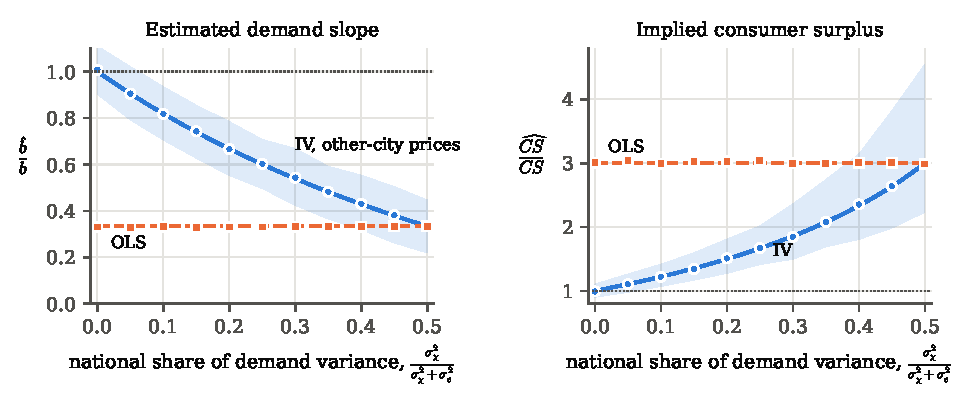
\includegraphics[width=\textwidth]{figures/ch10/hausman_iv_bias.pdf}
\caption{Hausman instruments with national demand shocks, a Monte Carlo experiment. The left panel shows the
estimated demand slope relative to the truth. The right panel shows the implied consumer surplus with linear
demand relative to the truth. Markers are Monte Carlo means (slope) or medians (surplus) over 500
replications. Lines are the probability limits of \cref{prop:10-hausman-iv-bias}, solid for IV and dashed for
OLS. The band shows the 10th to 90th percentiles of the IV estimates. The design has 7 cities, 137 weeks,
$b = 2$, $\sigma_\chi^2 + \sigma_e^2 = 1$ and $\sigma_k = \sigma_v = 0.5$. All shocks are anticipated, and city
fixed effects are removed. The script is \texttt{figures/ch10/src/hausman\_iv\_bias.py}.}
\label{fig:10-hausman-iv-mc}
\end{figure}

Two features of the experiment deserve comment. First, the instrument is strong throughout: the correlation
between a city's price and the other-city average is about 0.5 to 0.65. A strong first stage is no
protection against an invalid instrument. Second, week fixed effects cannot remove the problem for a single
product. They would absorb the national cost shocks as well, and with them all identifying variation. In a
system with many brands, week effects common to all brands absorb only aggregate shocks. Brand-specific
national shocks, the kind Bresnahan describes, remain.

\casehead{Evidence from later work}
\citet{Nevo2001} uses Hausman instruments for cereal in a random-coefficients model (\cref{ch:blp}). His
instruments are regional quarterly average prices of the same brand, excluding the city being instrumented
(p.~321). He discusses exactly Bresnahan's concern. A national demand shock, such as the discovery that fiber
reduces the risk of cancer, would raise the valuation of fiber-rich brands in all cities and violate the
assumption. He argues that the concern is weaker for well-established brands and that time dummies absorb
aggregate shocks. He then compares the price coefficient across instrument sets in his logit regressions
(Table V). With other-city prices it is $-17.57$ (0.50), and with proxies for local marginal cost it is
$-17.12$ (0.49), against $-7.26$ (0.16) by OLS with brand dummies. The two instrument sets agree. Nevo notes,
however, that regional demand shocks would invalidate both, and overidentification tests reject in all
columns except the one with city fixed effects. The comparison is informative, but it cannot rule out
brand-specific national shocks.

\subsection{Imperfect competition is ``off point''}\label{sec:10-bresnahan-competition}

Bresnahan's second criticism concerns economic interpretation (pp.~243--246). Imperfect competition links
new goods and market power in three ways. A new good can create market power for its inventor. It can
destroy market power of competing products. And the transitory market power that results is a reward that
motivates invention.

\casehead{Private returns}
The steep $dd$ that implies a large consumer surplus also implies a large monopoly rent if one firm owns the
product (p.~243). \Cref{rem:10-steep} makes this exact for linear demand, where consumer surplus at the
monopoly price is half the profit. Demand studies of new goods therefore speak to private returns to
innovation as well as social returns. With multiproduct firms and competitive responses, the calculation
needs the whole demand system and a supply model (p.~243).

\casehead{Rivals' prices}
Under imperfect competition among single-product firms, a new product lowers the market power of existing
products and so lowers prices (p.~243). This is one of the classical benefits of competition.
\Cref{sec:10-rival-prices} develops the argument. It proves the result for logit demand
(\cref{prop:10-logit-rivals}) and discusses Bresnahan's two qualifications, that unusual elasticities can
reverse it (fn.~12) and that Bertrand competition reinforces the direct effects (fn.~13).

Hausman holds the prices of Kellogg and Post fixed. Bresnahan calls this ``a common error among those who
are new to models of imperfect competition, but an important one'' (p.~244). The Bertrand solution concept
has firms maximize post-entry profits taking each other's post-entry prices as given. The analyst who
computes the effect of entry cannot take those prices as given, because entry changes the game. Typically
the rivals' prices fall. By holding them fixed, Hausman solves the price-discrimination problem of General
Mills as if it were a monopolist. His claim of a lower bound is therefore wrong, as Hausman's own fn.~32
partly concedes.

\casehead{The multiproduct firm's own prices}
Even for General Mills alone, the direction of the price change is ambiguous. Adding a brand changes the
first-order condition \eqref{eq:10-foc-elast} for an existing brand $j$ in the three ways of
\cref{sec:10-own-prices} (pp.~244--245). The new brand's term favors a higher $p_j$, which is the effect
Hausman stresses. Bresnahan counts the falls in the revenue shares of the existing brands, $w_j$ among them,
as the offsetting effects. At fixed margins and elasticities, only the cannibalization of the firm's other
brands pushes the other way, because it shrinks the positive cross terms. Bresnahan states that with linear demand and a two-product firm the effects exactly offset, and
\cref{prop:10-linear-offset} proves this for any number of products. Any dominance of one effect therefore
comes ``from higher-order derivatives'', and the paper offers no evidence on them (p.~245). The reproduction of Table 5.7 in
\cref{sec:10-hausman-imperfect} makes the point concrete. Hausman's ``without'' margins keep the post-launch
shares of Cheerios and Honey-Nut, so they include the first effect and omit the second and third.

\casehead{Where the action is}
Bresnahan summarizes the possibilities in the two-by-two classification of \cref{tab:10-bresnahan-2x2}.
Hausman's analysis sits in the price-discrimination cell. Bresnahan argues that if the social return is the object of interest, Hausman ``has
quantified the generally far less important effect'' (p.~246). The competition cell, the effect of a new
good on the pricing incentives of rival firms, must in general be much more important.

\casehead{Conclusion}
Bresnahan was left ``unconvinced by key econometric assumptions'' and found the imperfect-competition
analysis ``off point''. To doubt the large single-product surplus may simply be to believe in nationwide
brand-name demand shocks. ``The puzzle of the value of this incremental product introduction remains
unsolved'' (p.~246).

\subsection{Assessment}\label{sec:10-bresnahan-assessment}

Each side of the exchange got something right. Hausman showed that the exact value of a new brand can be
computed from estimated demand, and that a flexible system can deliver a finite virtual price. He also showed
that the answer depends on market structure. Bresnahan showed that the identifying assumption is strong
exactly where the conclusion is sensitive. Own-price slopes biased toward zero produce steep $dd$ curves and
large surplus. He also showed that holding rivals' prices fixed answers a monopoly question, and that the
multiproduct effect itself is ambiguous.

Several kinds of evidence could settle the dispute. Price and quantity data spanning the launch would allow
a direct before-and-after comparison, which Hausman lacked. \citet{HausmanLeonard2002} later made such a
comparison for Kleenex Bath Tissue (KBT), which Kimberly-Clark rolled out across U.S. cities in waves.\footnote{We
checked the numbers in this paragraph against the authors' revised manuscript dated September 1999 (pp.~10--15 and
33--36, and Tables~2, 6 and~7), which thanks the journal's referees and editor. We did not check the published article, whose
page and table numbers may differ.}
They use weekly Nielsen scanner data on the seven largest brands in 30 cities from January 1992 to September 1995.
KBT was already sold in 17 cities when the data begin. It entered three more in July 1993 and the last ten in May
1994. For each incumbent brand they estimate by ordinary least squares
\begin{equation}\label{eq:10-hl-direct}
  \ln p_{ct} = \lambda_c + \omega_t + \beta_1 I_{ct} + \beta_2 M_{ct} + e_{ct},
\end{equation}
where $c$ indexes cities and $t$ weeks, and $\lambda_c$ and $\omega_t$ are city and week fixed effects. The
indicator $I_{ct}$ equals one once KBT is sold in city $c$, and $M_{ct}$ marks the third-wave cities in the weeks
between the second and third waves. The staggered entry separates $\beta_1$ from the common shocks absorbed by
$\omega_t$. All six estimated price effects are negative (Table~2). Cottonelle fell 8.2 percent (standard error
1.3), Charmin and Angel Soft 3.5 percent, private label 3.8 percent and Northern 2.3 percent. The economy brand
ScotTissue fell only 0.6 percent (0.5). Kimberly-Clark had almost no prior share, so this is the competition cell
of Bresnahan's classification, and the prices of rivals fell as he predicts. The authors also predict these
changes from the post-entry demand system under Nash-Bertrand pricing. The predictions are close for four brands
but well short for Cottonelle ($-3.6$ percent) and private label ($-0.7$ percent), where $t$-tests reject equality
(Table~6). Because the comparison gives mixed support, they describe their evidence for Nash-Bertrand pricing as
cautious. The authors put the total consumer
gain at \$69.2 million a year, 7.3 percent of bath tissue spending in the 30 cities (Table~7). About half of it
comes from the lower prices of existing brands (p.~36).
Residuals of the same brand in different cities and the same week can be tested for correlation, the most
direct symptom of national shocks. Overidentification tests across cities, which fn.~20 of Hausman's paper
proposes, could be reported. Instruments from observed local costs offer a comparison, as in
\citet{Nevo2001}. Each check addresses a specific threat. None is a general proof of validity.

The broader literature moved in two directions. One kept product-space demand and looked for better
instruments and data. The other moved to characteristics space \citep{Berry1994,BerryLevinsohnPakes1995}.
There the value of a new product depends on its location relative to existing products, and instruments come
from the characteristics of rivals. That approach has its own extrapolation problem, the idiosyncratic
taste shock that gives every product a positive value, which \cref{sec:10-charspace} analyzes. It also has its
own instrument problem, the assumption that characteristics are exogenous (\cref{ch:discrete}).
\citet{Petrin2002}, studied in \cref{sec:10-petrin}, combines characteristics-space demand with micro data and
recomputes the full Bertrand equilibrium without the new product. His results quantify the competition cell of
Bresnahan's classification, together with the price-discrimination cell.

\section{Valuing new goods in characteristics space}\label{sec:10-charspace}

The methods of \cref{sec:10-virtual,sec:10-functional} value a new good in product space. They estimate the
demand curve of the good itself and integrate under it up to the virtual price. This section treats a product
as a bundle of characteristics instead, in the tradition of \citet{Lancaster1966,Lancaster1971} and
\citet{McFadden1981}. The change of viewpoint has three consequences for welfare measurement. First, a
characteristics model can predict the demand for a product that has never been sold. Second, discrete-choice
models deliver consumer surplus in closed form, so the value of a change in the choice set is a simple function
of estimated parameters. Third, the functional forms that make these models tractable carry strong implicit
assumptions about the value of variety. Most of the section makes those assumptions explicit and compares the
models that impose them with models that do not.

Throughout the section a market has inside products $j = 1,\dots,J$ and an outside good $j = 0$. Consumer $i$
has income $y_i$, and we use the notation of \cref{ch:logit,ch:blp} for mean utilities $\delta_j$, deviations
$\mu_{ij}$ and idiosyncratic shocks $\epsilon_{ij}$. Where we discuss \citet{Trajtenberg1989}, we write
$\mathcal{W}(S)$ for his surplus function over a choice set $S$. We also write $z_j$ for the vector of
characteristics of product $j$ and $\tilde p_j$ for its residual price relative to a hedonic price function.

\subsection{Predicting demand for products that have never been sold}\label{sec:10-cs-predict}

A new product is a new point in characteristics space. Suppose a demand model has been estimated on existing
products, and the new product combines characteristics that lie within the range spanned by them. The estimated
tastes for characteristics then predict the new product's market share at any price, and the equilibrium pricing
conditions of \cref{ch:diffprod} predict its price. A product-space system cannot do this, because its
parameters are indexed by products and the new product has none \citep[pp.~1--2]{BerryPakes2007}. Berry and
Pakes add a second advantage. The number of parameters of a characteristics model does not grow with the number
of products. A log-linear product-space system for $J$ products needs a number of parameters of the order of $J^2$. \Citet{BerryLevinsohnPakes2004} use this property to simulate the demand for products before launch.

The same property disciplines the retrospective valuation of products that already exist. We never observe
demand at prices high enough to reveal the reservation prices of most buyers. Every estimate of the surplus
from a product therefore extrapolates beyond the data \citep[p.~2]{BerryPakes2007}. A product-space system extrapolates the
product's own demand curve to high prices, as in \cref{sec:10-functional}. A characteristics model uses slightly
more information. It borrows the price variation of other products with similar characteristics, although the
functional form still governs the extrapolation.

The approach has three limits. The first is an \emph{entirely new characteristic}, one that no existing product
possesses. Tastes for it cannot be learned from existing products. An electric car, for example, has a range, a
charging time and no fuel cost, so its demand cannot be inferred from the demand for gasoline cars alone. The
second limit is attributes that resist measurement, such as the plot of a book or the style of a film. When the
relevant attributes cannot be coded as a short vector $x_j$, the approach loses its dimension reduction. The third
limit is the \emph{radical innovation}, a product that opens a new product class. \Citet[pp.~10--11]{Trajtenberg1985}\footnote{We cite
\citet{Trajtenberg1989} through its working-paper version \citep{Trajtenberg1985}, the text available to us. Page,
table and equation numbers for this study refer to the working paper, as explained in \cref{sec:10-trajtenberg}.}
argues that a welfare comparison requires a choice set and a surplus function defined before the innovation, and
a radical innovation offers neither. He quotes \citet[p.~28]{Kuznets1962} on the point. For Kuznets, a rough
estimate of the value of a new product ``seems to be possible only if the new product can be treated as a substitute
for the old one.''
Trajtenberg's response is to measure the improvements that follow the first commercial product, and to infer the
value of the first product indirectly from the diffusion of the innovation (\cref{sec:10-ct-diffusion}).

\Citet[p.~229]{Hausman1997} pushes the first two limits further, as \cref{sec:10-hausman-ces} reports. He
describes each cereal brand by its own indicator variable and doubts that a brand such as Apple-Cinnamon Cheerios
can be described by its attributes. For him the natural measure of distance between products is the cross-price
elasticity. \Citet[p.~238, n.~3]{Bresnahan1997} reads the characteristics approach more favorably. Trajtenberg used
an address model of differentiation. This led him to conjecture that a new good's distance from existing products
governs the slope of its demand curve $dd$, and hence its surplus (\cref{fig:10-dd-DD}). The propositions below
make this conjecture precise for the logit, the nested logit and the vertical model.

Finally, the characteristics models used in this section assume that each consumer buys one unit of one product.
Products can then only be substitutes. Complementarity between a new good and old goods requires a model of
bundles, which we study in \cref{sec:10-gentzkow}.

\subsection{Consumer surplus in random utility models}\label{sec:10-cs-welfare}

We begin with the welfare theory that all characteristics-based valuations share. The key assumption is that
income enters utility linearly, so that utility differences convert into money at a constant rate.

\begin{assumption}[Quasi-linear random utility]\label{ass:10-quasilinear}
Consumer $i$'s utility from product $j\in\{1,\dots,J\}$ and from the outside good are
\begin{equation}\label{eq:10-quasilinear}
u_{ij} = \alpha(y_i - p_j) + x_j\beta + \xi_j + \mu_{ij} + \epsilon_{ij},
\qquad
u_{i0} = \alpha y_i + \epsilon_{i0},
\end{equation}
with $\alpha > 0$. Write $\delta_j = x_j\beta - \alpha p_j + \xi_j$ and set $\delta_0 = \mu_{i0} = 0$. The shocks
$(\epsilon_{i0},\dots,\epsilon_{iJ})$ are independent of $(x,\xi,\mu_i)$, have a joint density and a finite mean.
In the logit case they are \iid\ type-I extreme value.
\end{assumption}

The term $\alpha y_i$ is common to all alternatives, so it does not affect choices. For a consumer with deviations
$\mu_i$, define the \emph{expected maximum utility} over a choice set $\mathcal{J}$ that contains the outside good,
\begin{equation}\label{eq:10-emax}
G_i(\mathcal{J}) = \E\left[\max_{j\in\mathcal{J}}\left(\delta_j + \mu_{ij} + \epsilon_{ij}\right)\right],
\end{equation}
where the expectation is over $\epsilon_i$.

\begin{lemma}[Compensating variation under quasi-linearity]\label{lem:10-cv-quasilinear}
Under \cref{ass:10-quasilinear}, let the choice set and prices change from $(\mathcal{J}^0,p^0)$ to
$(\mathcal{J}^1,p^1)$. Let $CV_i$ be the extra income that consumer $i$ would need, facing $(\mathcal{J}^0,p^0)$, to
reach the utility she attains at $(\mathcal{J}^1,p^1)$, as in \cref{def:10-cv}. For every realization of $\epsilon_i$,
\begin{equation}\label{eq:10-cv-draw}
CV_i = \frac{1}{\alpha}\left[\max_{j\in\mathcal{J}^1}\left(\delta^1_j + \mu_{ij} + \epsilon_{ij}\right)
- \max_{j\in\mathcal{J}^0}\left(\delta^0_j + \mu_{ij} + \epsilon_{ij}\right)\right],
\end{equation}
and the expected compensating variation is $\E[CV_i] = \frac{1}{\alpha}\left[G^1_i(\mathcal{J}^1) -
G^0_i(\mathcal{J}^0)\right]$, where $G^t_i$ uses the mean utilities $\delta^t$.
\end{lemma}

\begin{proof}
Adding $c$ to income before the change raises the utility of every alternative by $\alpha c$. The maximal utility
before the change, with the extra income, is therefore
\begin{equation*}
\alpha(y_i + c) + \max_{j\in\mathcal{J}^0}\left(\delta^0_j + \mu_{ij} + \epsilon_{ij}\right).
\end{equation*}
After the change, maximal utility is $\alpha y_i + \max_{j\in\mathcal{J}^1}(\delta^1_j + \mu_{ij} + \epsilon_{ij})$.
Setting the two equal and solving for $c$ gives \eqref{eq:10-cv-draw}. Taking expectations over $\epsilon_i$ gives
the second statement.
\end{proof}

Because income effects are absent, the compensating and equivalent variations coincide here. Under quasi-linearity
we therefore call $\frac{1}{\alpha}G_i(\mathcal{J})$, up to a constant, the \emph{expected consumer surplus}
$CS_i(\mathcal{J})$. This is the measure of \citet{SmallRosen1981} and \citet{McFadden1981}. The next lemma shows
that it is the integral under the demand curves, so it is the discrete-choice counterpart of the Hicksian area in
\cref{prop:10-cv-newgood}.

\begin{lemma}[Williams-Daly-Zachary, \citealp{McFadden1981}]\label{lem:10-wdz}
Let $\epsilon = (\epsilon_0,\dots,\epsilon_J)$ have a joint density and a finite mean, and let
$G(\delta) = \E[\max_k(\delta_k + \epsilon_k)]$. Then $G$ is differentiable and
$\frac{\partial G}{\partial \delta_j} = \Pr\left(j = \argmax_k(\delta_k + \epsilon_k)\right)$ for every $j$.
\end{lemma}

The lemma restates part (ii) of \cref{thm:06-wdz} with $V = \delta$. The proof there bounds the difference
quotient of the maximum by one and applies dominated convergence.

Two consequences follow. Since $\delta_j$ contains $-\alpha p_j$, the chain rule gives
\begin{equation}\label{eq:10-roy}
\frac{\partial CS_i}{\partial p_j} = \frac{1}{\alpha}\,\frac{\partial G_i}{\partial \delta_j}\,(-\alpha) = -s_{ij},
\end{equation}
where $s_{ij}$ is consumer $i$'s choice probability. This is Roy's identity for discrete choice, and
\citet[p.~19, n.~18]{Trajtenberg1985} uses it to verify his surplus function. Consumer surplus is thus the area under
the probabilistic demand curves, and the change in $CS_i$ from raising $p_n$ to infinity is the area under
product $n$'s demand curve. The second consequence is a closed form in the logit case.

\begin{lemma}[Log-sum formula]\label{lem:10-logsum}
If $\epsilon_0,\dots,\epsilon_J$ are \iid\ type-I extreme value, then $\max_k(\delta_k + \epsilon_k)$ is
type-I extreme value with location $\ln\sum_{k=0}^{J} e^{\delta_k}$, and
\begin{equation}\label{eq:10-logsum}
\E\left[\max_k(\delta_k + \epsilon_k)\right] = \ln\sum_{k=0}^{J} e^{\delta_k} + \gamma_E,
\end{equation}
where $\gamma_E \approx 0.5772$ is Euler's constant.
\end{lemma}

The first statement is the max-stability of the Gumbel distribution (\cref{lem:06-maxstable}). The second is
\cref{prop:06-logsum} with $V_{ik} = \delta_k$ and $\sigma_\epsilon = 1$.

With $\delta_0 = 0$, the logit consumer surplus is therefore
\begin{equation}\label{eq:10-logit-cs}
CS = \frac{1}{\alpha}\ln\left(1 + \sum_{k=1}^{J}e^{\delta_k}\right) + C,
\end{equation}
where $C$ collects income and $\gamma_E$ and does not depend on the choice set. \Cref{sec:06-tiev} derives the
extreme value algebra and the logit shares. Trajtenberg's surplus function is the
same object, $\mathcal{W}(S) = \frac{1}{\alpha}\ln\sum_{j\in S}e^{V_j}$, written for a choice set $S$ of scanners
without an outside good. We now use \eqref{eq:10-logit-cs} to value an introduction.

\begin{proposition}[Value of a new product in the logit model]\label{prop:10-logit-newgood}
In the logit model, add product $n$ with mean utility $\delta_n$ to a market with products $1,\dots,J$, holding
the other mean utilities fixed. Per consumer, consumer surplus rises by
\begin{equation}\label{eq:10-logit-newgood}
\Delta CS = \frac{1}{\alpha}\ln\left(1 + \frac{e^{\delta_n}}{1 + \sum_{k=1}^{J}e^{\delta_k}}\right)
= -\frac{1}{\alpha}\ln(1 - s_n),
\end{equation}
where $s_n$ is the market share of product $n$ after the introduction.
\end{proposition}

\begin{proof}
The introduction reverses the removal of $n$ from the post-introduction market. By \eqref{eq:07-removal-logit} in
\cref{cor:07-removal}, that removal changes surplus by $\frac{1}{\alpha}\ln(1 - s_n)$, with $s_n$ the share before
the removal, which is the share after the introduction. The introduction therefore raises surplus by
$-\frac{1}{\alpha}\ln(1 - s_n)$. For the first expression, let $A_0 = 1 + \sum_{k=1}^{J}e^{\delta_k}$ and
$A_1 = A_0 + e^{\delta_n}$. Then $s_n = \frac{e^{\delta_n}}{A_1}$, so $1 - s_n = \frac{A_0}{A_1}$ and
$-\ln(1 - s_n) = \ln\frac{A_1}{A_0} = \ln\big(1 + \frac{e^{\delta_n}}{A_0}\big)$.
\end{proof}

The proposition has a strong implication. The value of a new product depends only on its share and on the
price coefficient. Two products with the same share are worth the same, whether one is a novel design and the
other a near copy of an existing product. The characteristics of the new product matter only through the share
they produce. The CES variety index of \cref{cor:10-ces-newgood} has the same property, since it depends only on
the new good's expenditure share and the elasticity of substitution. \Cref{rem:10-ces-logit} explains why the
two results are close relatives: the CES demand system is the aggregate demand of logit consumers
\citep{AndersonDePalmaThisse1992}.

The proposition also bounds the gain of the average buyer of the new product. For $s \in (0,1)$ we have
$s \le -\ln(1 - s) \le \frac{s}{1-s}$, by the series $-\ln(1-s) = \sum_{m\ge1}\frac{s^m}{m}$. Dividing
\eqref{eq:10-logit-newgood} by $s_n$ therefore gives
\begin{equation}\label{eq:10-logit-perbuyer}
\frac{1}{\alpha} \le \frac{\Delta CS}{s_n} \le \frac{1}{\alpha(1 - s_n)} .
\end{equation}
The upper bound is the markup of a single-product logit firm (\cref{prop:10-clones} below). So in the logit
model the average buyer of a new product gains at least $\frac{1}{\alpha}$ dollars, however close the product is
to existing ones. She gains roughly as much as the firm earns per unit sold. For a small share, $\Delta CS \approx
\frac{s_n}{\alpha}$. The market-level gain is $M\,\Delta CS$ for a market of size $M$. If the introduction also
changes rivals' prices, as in \cref{prop:10-logit-rivals}, the formula measures the variety effect at the new
prices, and the price effect must be added.

Nesting relaxes the result in the direction that \citet{Bresnahan1997} and Trajtenberg anticipate. Partition the
inside products into nests $g = 1,\dots,G$ and place the outside good in its own nest. In the nested logit of
\cref{ch:logit}, with nesting parameter $\sigma\in[0,1)$, define the inclusive value sums
$D_g = \sum_{j\in g}e^{\frac{\delta_j}{1-\sigma}}$. Shares and consumer surplus are
\begin{equation}\label{eq:10-nl-shares}
s_{j|g} = \frac{e^{\frac{\delta_j}{1-\sigma}}}{D_g},
\qquad
s_g = \frac{D_g^{1-\sigma}}{1 + \sum_{h=1}^{G}D_h^{1-\sigma}},
\qquad
CS = \frac{1}{\alpha}\ln\left(1 + \sum_{h=1}^{G}D_h^{1-\sigma}\right) + C .
\end{equation}

\begin{proposition}[Value of a new product in the nested logit model]\label{prop:10-nested-newgood}
In the nested logit model \eqref{eq:10-nl-shares}, add product $n$ to nest $g$, holding the other mean utilities
fixed. Per consumer, consumer surplus rises by
\begin{equation}\label{eq:10-nested-newgood}
\Delta CS = -\frac{1}{\alpha}\ln\left[1 - s_g + s_g\left(1 - s_{n|g}\right)^{1-\sigma}\right],
\end{equation}
where $s_g$ is the share of nest $g$ and $s_{n|g}$ the within-nest share of product $n$, both after the
introduction. For fixed post-introduction shares, $\Delta CS$ equals the logit value $-\frac{1}{\alpha}\ln(1-s_n)$
at $\sigma = 0$, falls strictly as $\sigma$ rises, and tends to zero as $\sigma\to 1$.
\end{proposition}

\begin{proof}
Let primes denote post-introduction values. Only nest $g$ changes:
$D_g' = D_g + e^{\frac{\delta_n}{1-\sigma}}$. Since $s_{n|g} = \frac{e^{\frac{\delta_n}{1-\sigma}}}{D_g'}$, we have
\begin{equation*}
D_g = D_g' - e^{\frac{\delta_n}{1-\sigma}} = D_g'\left(1 - s_{n|g}\right).
\end{equation*}
Write $A' = 1 + \sum_h D_h'^{1-\sigma}$ and $A = 1 + \sum_h D_h^{1-\sigma}$. Then
\begin{equation*}
A = A' - D_g'^{1-\sigma} + D_g^{1-\sigma} = A' - D_g'^{1-\sigma} + D_g'^{1-\sigma}\left(1 - s_{n|g}\right)^{1-\sigma}.
\end{equation*}
Dividing by $A'$ and using $s_g = \frac{D_g'^{1-\sigma}}{A'}$ gives
\begin{equation*}
\frac{A}{A'} = 1 - s_g + s_g\left(1 - s_{n|g}\right)^{1-\sigma}.
\end{equation*}
Since $\Delta CS = \frac{1}{\alpha}\ln\frac{A'}{A} = -\frac{1}{\alpha}\ln\frac{A}{A'}$, \eqref{eq:10-nested-newgood}
follows. At $\sigma = 0$ the bracket is $1 - s_g s_{n|g} = 1 - s_n$. Because $0 < 1 - s_{n|g} < 1$, the term
$(1 - s_{n|g})^{1-\sigma}$ rises strictly with $\sigma$ and tends to 1. The bracket therefore rises toward 1, and
$\Delta CS$ falls toward zero.
\end{proof}

The nesting parameter measures how close the new product is to the other members of its nest. At $\sigma = 0$
every product is an equally distant substitute and the logit value applies. As $\sigma \to 1$ the products within
a nest become perfect substitutes, and a new member of a crowded nest adds nothing. This is Bresnahan's point about
the slope of $dd$ in discrete-choice form. A new product that steals its share from close substitutes has a flat
demand curve and little surplus. With $s_g = 0.3$ and $s_{n|g} = 0.1$, for example, the gain in units of
$\frac{1}{\alpha}$ is 0.0305 at $\sigma = 0$, 0.0155 at $\sigma = 0.5$ and 0.0032 at $\sigma = 0.9$.

Trajtenberg writes the nested logit in a different but equivalent way, which matters for reading his estimates.
His within-nest index is $V_j = \frac{\delta_j}{1-\sigma}$, so the within-nest shares are $s_{j|g} =
\frac{e^{V_j}}{\sum_{k\in g}e^{V_k}}$. His nest-level parameter is $\lambda = 1 - \sigma$, and the inclusive value
of nest $g$ is $W_g = \ln\sum_{k\in g}e^{V_k}$. The nest shares are $s_g = \frac{e^{a_g + \lambda
W_g}}{\sum_h e^{a_h + \lambda W_h}}$, where we have added nest constants $a_g$ that his specification sets to
zero. In a sequential estimator, the coefficients inside $V_j$ are estimated in a first stage and then held fixed.
Let $\alpha_V = \frac{\alpha}{\lambda}$ denote the price coefficient inside $V_j$. Differentiating $\ln s_j =
V_j - W_g + a_g + \lambda W_g - \ln\sum_h e^{a_h+\lambda W_h}$ gives, for $j\in g$,
\begin{equation}\label{eq:10-nl-semi}
\frac{\partial\ln s_j}{\partial V_k} =
\begin{cases}
-s_{k|g}\left[1 - \lambda(1 - s_g)\right], & k\in g,\ k\ne j,\\[2pt]
-\lambda\, s_k, & k\in h \ne g .
\end{cases}
\end{equation}
Holding the $V$'s fixed, $\lambda\to0$ drives the cross-nest effects to zero while the within-nest effects stay
bounded away from zero. In this parameterization a small $\lambda$ therefore means that the nests are separate
markets, which is the reading \citet[p.~43, n.~42]{Trajtenberg1985} gives it. With $\delta_j$ held fixed instead,
$\sigma\to1$ makes products within a nest perfect substitutes. The two readings differ only in what is held
fixed. The money value of a change in the inclusive values has a simple limit.

\begin{corollary}[Separate markets]\label{cor:10-separate-markets}
In the parameterization above, consumer surplus is $CS = \frac{1}{\lambda\alpha_V}\ln\sum_h e^{a_h + \lambda W_h}
+ C$. Let the inclusive values change from $W^0_h$ to $W^1_h$, and let $s^0_h = \frac{e^{a_h}}{\sum_m e^{a_m}}$.
Holding $\alpha_V$, the $a_h$ and the $W$'s fixed, as $\lambda\to 0$
\begin{equation}\label{eq:10-separate-markets}
\Delta CS \;\to\; \sum_h s^0_h\,\frac{W^1_h - W^0_h}{\alpha_V}.
\end{equation}
\end{corollary}

\begin{proof}
In the units of $\delta$, the marginal utility of income is $\alpha = \lambda\alpha_V$, and nest-level consumer
surplus is $\frac{1}{\alpha}\ln\sum_h e^{a_h + \lambda W_h}$ by the nested version of \cref{lem:10-logsum}. Define
$f(\lambda) = \ln\sum_h e^{a_h + \lambda W^1_h} - \ln\sum_h e^{a_h + \lambda W^0_h}$, so that $\Delta CS =
\frac{f(\lambda)}{\lambda\alpha_V}$. Then $f(0) = 0$ and
\begin{equation*}
f'(0) = \sum_h \frac{e^{a_h}}{\sum_m e^{a_m}}\,W^1_h - \sum_h \frac{e^{a_h}}{\sum_m e^{a_m}}\,W^0_h
= \sum_h s^0_h\left(W^1_h - W^0_h\right).
\end{equation*}
By l'H\^opital's rule, $\frac{f(\lambda)}{\lambda}\to f'(0)$, which gives \eqref{eq:10-separate-markets}.
\end{proof}

When the nests are separate markets, the nest shares no longer respond to the products, and the value of a change
is the share-weighted average of the within-nest log-sum changes. This is exactly how Trajtenberg aggregates the
gains in head and body scanners (\cref{sec:10-ct-welfare}).

\casehead{Random coefficients and income effects} With random coefficients the logit formula holds consumer by
consumer. Conditional on $(D_i,\nu_i)$, the logit form gives $CS_i = \frac{1}{\alpha_i}\ln(1 + \sum_k
e^{\delta_k + \mu_{ik}})$, and the market measure integrates this over the distribution of $(D_i,\nu_i)$, as in
\cref{ch:blp}. Income effects break the log-sum formula. \Citet{Petrin2002} uses $\alpha_i\ln(y_i - p_j)$ in place
of $\alpha(y_i - p_j)$, so the marginal utility of income varies with $y_i - p_j$. Let the introduction change the
choice set from $\mathcal{J}^0$ at prices $p^0$ to $\mathcal{J}^1$ at prices $p^1$. With the standard of living
after the introduction as the reference, as in \cref{def:10-cv}, the compensating variation of consumer $i$ solves
\begin{equation}\label{eq:10-cv-income}
\max_{j\in\mathcal{J}^0}u_{ij}\left(y_i + CV_i,\, p^0\right) = \max_{j\in\mathcal{J}^1}u_{ij}\left(y_i,\, p^1\right).
\end{equation}
It depends on the realized tastes, and its average over consumers is computed by simulation.
\begin{enumerate}
\item Draw $R$ simulated consumers. For each draw $r$, draw demographics $D_r$ from their empirical distribution,
taste shocks $\nu_r$, and an extreme value shock $\epsilon_{rj}$ for every product in $\mathcal{J}^0\cup
\mathcal{J}^1$. Use the same $\epsilon_{rj}$ for a product in both choice sets.
\item Compute the new maximal utility $\bar u_r = \max_{j\in\mathcal{J}^1}u_{rj}(y_r, p^1)$.
\item Find $CV_r$ by bisection on $c\mapsto\max_{j\in\mathcal{J}^0}u_{rj}(y_r + c, p^0) - \bar u_r$. This
function is continuous and strictly increasing in $c$, because utility rises with income for every product.
\item Average: $\widehat{\E[CV]} = \frac{1}{R}\sum_r CV_r$. Multiply by the market size for the total.
\end{enumerate}
For Petrin's logarithmic specification, step 3 even has a closed form, derived in \cref{sec:10-petrin-cv}. Other
income specifications need the root finder.
The average of the individual $CV_r$ differs in general from the income change that equates expected maximal
utilities. The two coincide under quasi-linearity, where $CV_r$ is linear in the utility difference.
\Cref{sec:10-petrin} applies this algorithm to the minivan and splits the result into a part due to observed
characteristics and a part due to the $\epsilon$'s.

\subsection{The idiosyncratic-taste problem}\label{sec:10-cs-epsilon}

Characteristics-based demand models fall into two families, and the difference between them drives the valuation
of new goods. Let $f(y_i,p_j)$ be a function with $f_y > 0$, $f_p < 0$ and $f_{py}\ge 0$, so that utility rises
with income, falls with price, and richer consumers are weakly less sensitive to price. The first family contains
the \emph{pure characteristics models},
\begin{equation}\label{eq:10-pure-classes}
U_{ij} = f(y_i,p_j) + \delta_j + \sum_k\beta_k x_{jk}\nu_{ik}
\qquad\text{or}\qquad
U_{ij} = f(y_i,p_j) + \delta_j - \sum_k\tau_k\left(x_{jk} - \nu_{ik}\right)^2 ,
\end{equation}
with $\tau_k > 0$. The first form is the pure hedonic model of \citet{BerryPakes2007}, in which $\nu_{ik}$ is a
taste for characteristic $k$. The second is the ideal-type model of \citet{AndersonDePalmaThisse1992}, in which
$\nu_{ik}$ is consumer $i$'s ideal level of characteristic $k$. The second family adds an idiosyncratic shock,
\begin{equation}\label{eq:10-blp-class}
U_{ij} = f(y_i,p_j) + \delta_j + \sum_k\beta_k x_{jk}\nu_{ik} + \epsilon_{ij},
\end{equation}
as in \citet{BerryLevinsohnPakes1995}. The shocks $\epsilon_{ij}$ are drawn independently for every product and
consumer. \Citet{BerryPakes2007} call the second family models with \emph{tastes for products}, because the
$\epsilon_{ij}$ act like a separate characteristic for each product. Following \citet{CaplinNalebuff1991}, one
can think of them as interactions between product-specific dummy variables and \iid\ tastes for each dummy.

The $\epsilon_{ij}$ mean that the product space can never be exhausted. Each new product arrives with a fresh set
of draws, so some consumers like it more than anything else on the market, whatever its observed characteristics.
The following proposition collects the implications for the logit.

\begin{proposition}[Clones in the logit model]\label{prop:10-clones}
In the logit model with $\delta_0 = 0$:
\begin{enumerate}[label=(\alph*)]
\item A \emph{clone} of product $j$, a new product with $\delta_n = \delta_j$, has a positive share and raises
consumer surplus by
\begin{equation}\label{eq:10-clone-gain}
\Delta CS = \frac{1}{\alpha}\ln\frac{1 + \sum_{k=1}^{J}e^{\delta_k} + e^{\delta_j}}{1 + \sum_{k=1}^{J}e^{\delta_k}}
= \frac{1}{\alpha}\ln\left(1 + s^0_j\right) > 0,
\end{equation}
where $s^0_j$ is product $j$'s share before the clone enters.
\item With $J$ identical products of mean utility $\delta$, $CS(J) = \frac{1}{\alpha}\ln(1 + Je^{\delta}) + C$,
and $CS(J) - \frac{1}{\alpha}\ln J \to \frac{\delta}{\alpha} + C$. Consumer surplus grows like
$\frac{1}{\alpha}\ln J$ without bound.
\item The equilibrium markup of a single-product firm satisfies $p_j - mc_j = \frac{1}{\alpha(1 - s_j)} \ge
\frac{1}{\alpha}$, however many products crowd the market.
\item Every product with finite $\delta_j$ has a positive share, so the model cannot rationalize a product with a
zero share.
\end{enumerate}
\end{proposition}

\begin{proof}
(a) Apply \eqref{eq:10-logit-cs} with $A_0 = 1 + \sum_k e^{\delta_k}$ and $A_1 = A_0 + e^{\delta_j}$. Then
$\frac{A_1}{A_0} = 1 + \frac{e^{\delta_j}}{A_0} = 1 + s^0_j$, which exceeds 1.
(b) With $J$ identical products, $\sum_k e^{\delta_k} = Je^{\delta}$. Then
\begin{equation*}
\frac{1}{\alpha}\ln(1 + Je^{\delta}) - \frac{1}{\alpha}\ln J = \frac{1}{\alpha}\ln\left(\frac{1}{J} + e^{\delta}\right)
\to \frac{\delta}{\alpha}.
\end{equation*}
(c) Firm $j$ maximizes $(p_j - mc_j)Ms_j$. The logit share derivative is $\frac{\partial s_j}{\partial p_j} =
-\alpha s_j(1 - s_j)$. The first-order condition is
\begin{equation*}
s_j - (p_j - mc_j)\,\alpha s_j(1 - s_j) = 0 ,
\end{equation*}
so $p_j - mc_j = \frac{1}{\alpha(1-s_j)}$. Since $0 < s_j < 1$, the markup exceeds $\frac{1}{\alpha}$.
(d) $s_j = \frac{e^{\delta_j}}{1 + \sum_k e^{\delta_k}} > 0$ for finite $\delta_j$.
\end{proof}

Each part is unrealistic in some markets. Part (a) is the red bus and blue bus problem of \cref{ch:logit} viewed
from the welfare side. Adding a blue bus identical to a red bus creates surplus in the logit, although nothing new
is offered. Part (b) says that proliferating near-identical brands raises welfare without bound. Part (c) says that
markups do not fall toward marginal cost as the product space fills. In a pure characteristics model, by contrast,
a clone is a perfect substitute for the original. At given prices it adds no variety value. If a rival sells it,
Bertrand competition drives both prices to cost, and consumers gain only through this price effect. If the
original's owner sells it, nothing changes. Part (d) is the mirror image of the others. The model must assign every
product a positive share, so it cannot use the information in products that sell nothing, and the inversion $\ln
s_j - \ln s_0 = \delta_j$ breaks down at zero shares. The same mechanism biases estimated markups and the
estimated welfare gains from new goods upward.

\citet[p.~18]{Trajtenberg1985} noticed the welfare side of this problem in 1985. He decomposed his surplus function
into a part due to observed utility and a part due to dispersion.

\begin{proposition}[Entropy decomposition]\label{prop:10-entropy}
Let $s_j = \frac{e^{V_j}}{\sum_k e^{V_k}}$ be logit choice probabilities over a finite choice set. Then
\begin{enumerate}[label=(\alph*)]
\item $\ln\sum_j e^{V_j} = \sum_j s_jV_j + \mathcal{H}(s)$, where $\mathcal{H}(s) = -\sum_j s_j\ln s_j$ is the
\emph{entropy} of the choice probabilities.
\item Conditional on choosing $j$, the maximal utility $V_j + \epsilon_j$ is type-I extreme value with location
$\ln\sum_k e^{V_k}$, for every $j$. Hence
\begin{equation*}
\E[\epsilon_j\mid j\text{ chosen}] = \gamma_E - \ln s_j
\qquad\text{and}\qquad
\mathcal{H}(s) = \sum_j s_j\left(\E[\epsilon_j\mid j\text{ chosen}] - \gamma_E\right).
\end{equation*}
\end{enumerate}
\end{proposition}

\begin{proof}
(a) For every $j$, $\ln s_j = V_j - \ln\sum_k e^{V_k}$, so $\ln\sum_k e^{V_k} = V_j - \ln s_j$. Multiply by $s_j$
and sum over $j$. Since $\sum_j s_j = 1$,
\begin{equation*}
\ln\sum_k e^{V_k} = \sum_j s_jV_j - \sum_j s_j\ln s_j .
\end{equation*}
(b) Let $f$ and $F$ be the type-I extreme value density and CDF, and let $A = \sum_k e^{V_k - V_j} =
\frac{1}{s_j}$. The event that $j$ is chosen and its utility is at most $m$ has probability
\begin{equation*}
\int_{-\infty}^{m - V_j} f(e)\prod_{k\ne j}F(V_j + e - V_k)\,de
= \int_{-\infty}^{m - V_j} e^{-e}\exp\left(-e^{-e}A\right)de .
\end{equation*}
Substitute $t = e^{-e}$, so $dt = -e^{-e}de$. The integral becomes
\begin{equation*}
\int_{e^{-(m - V_j)}}^{\infty}e^{-tA}\,dt = \frac{1}{A}\exp\left(-Ae^{-(m-V_j)}\right)
= s_j\exp\left(-e^{-\left(m - \ln\sum_k e^{V_k}\right)}\right).
\end{equation*}
Dividing by $\Pr(j\text{ chosen}) = s_j$ gives the conditional CDF, which does not depend on $j$. Its mean is
$\ln\sum_k e^{V_k} + \gamma_E$, so $\E[\epsilon_j\mid j] = \ln\sum_k e^{V_k} - V_j + \gamma_E = \gamma_E - \ln s_j$.
Multiplying by $s_j$ and summing gives the last identity.
\end{proof}

Part (a) is Trajtenberg's equation (11), and part (b) explains what the entropy term measures. The surplus
function equals the share-weighted observed utility $\sum_j s_jV_j$ plus the average idiosyncratic taste that
consumers realize on the products they choose. With $J$ identical products and no outside good,
$\sum_j s_jV_j = V$ and $\mathcal{H} = \ln J$, so the entire gain from proliferation is entropy. Trajtenberg
traces this taste for ``horizontal variety'' to the independence of irrelevant alternatives. He notes that it
rewards ``the proliferation of seemingly identical brands that may differ only in their unobserved (and thus
presumably less important) attributes'' \citep[p.~19]{Trajtenberg1985}. For some purposes he suggests netting
out the change in entropy and using $\Delta\mathcal{W} - \frac{1}{\alpha}\Delta\mathcal{H}$. The net measure is not
a clean fix. The entropy term also contains the real value of matching heterogeneous buyers to different
products, which a model with random coefficients would attribute to observed characteristics.

Whether the $\epsilon$'s should count at all depends on what they represent. Four interpretations are common. They
may be tastes for unobserved product attributes, measurement error, approximation error in the utility function,
or optimization mistakes. Only the first supports counting them as welfare. If consumers choose with errors, the
log-sum formula counts the errors as utility.

\casehead{How the value of variety grows} \Cref{fig:10-variety-value} compares the growth of consumer surplus as
identical or evenly spaced products are added, in four models. The two logit-based curves use
\cref{prop:10-clones,prop:10-nested-newgood}. In the nested logit, $J$ identical products in one nest give
$D^{1-\sigma} = J^{1-\sigma}e^{\delta}$, so $CS(J) = \frac{1}{\alpha}\ln(1 + J^{1-\sigma}e^{\delta})$. Surplus still
grows without bound, at the slower rate $\frac{1-\sigma}{\alpha}\ln J$.

The pure characteristics benchmark is a Hotelling line. Consumers are uniform on $[0,1]$ and each buys one unit
at a common price $p$ from the nearest of $J$ products. The products sit at $\ell_k = \frac{2k-1}{2J}$, and a
consumer at distance $d$ from her product loses $td^2$. Each product serves an interval of length $\frac{1}{J}$,
and within it the distance $d$ is uniform on $\left[0,\frac{1}{2J}\right]$. The average loss is therefore
\begin{equation*}
t\,\E[d^2] = t\cdot\frac{1}{3}\left(\frac{1}{2J}\right)^2 = \frac{t}{12J^2},
\end{equation*}
and with gross value $v$,
\begin{equation}\label{eq:10-hotelling-cs}
CS(J) = v - p - \frac{t}{12J^2},
\qquad
CS(J) - CS(1) = \frac{t}{12}\left(1 - \frac{1}{J^2}\right) \le \frac{t}{12}.
\end{equation}
The gain is bounded, and the increment from one more product, $\frac{t}{12}\left(\frac{1}{J^2} -
\frac{1}{(J+1)^2}\right)$, falls to zero like $\frac{t}{6J^3}$. Adding logit errors with scale $\mu$ to the same
line gives $CS(x) = \mu\ln\sum_k e^{-\frac{t(x - \ell_k)^2}{\mu}}$ for a consumer at $x$, up to a constant. The
sum divided by $J$ is a Riemann sum, so for large $J$ the sum is close to
$J\,I(x)$ with $I(x) = \int_0^1 e^{-\frac{t(x - \ell)^2}{\mu}}\,d\ell > 0$. Hence $CS(x) \approx \mu\ln J + \mu\ln I(x)$,
and the gain grows like $\mu\ln J$. The integral $I(x)$ is close to the whole-line value $\sqrt{\frac{\pi\mu}{t}}$
only when both $x$ and $1 - x$ are large relative to $\sqrt{\frac{\mu}{t}}$.

\begin{figure}[htbp]
\centering
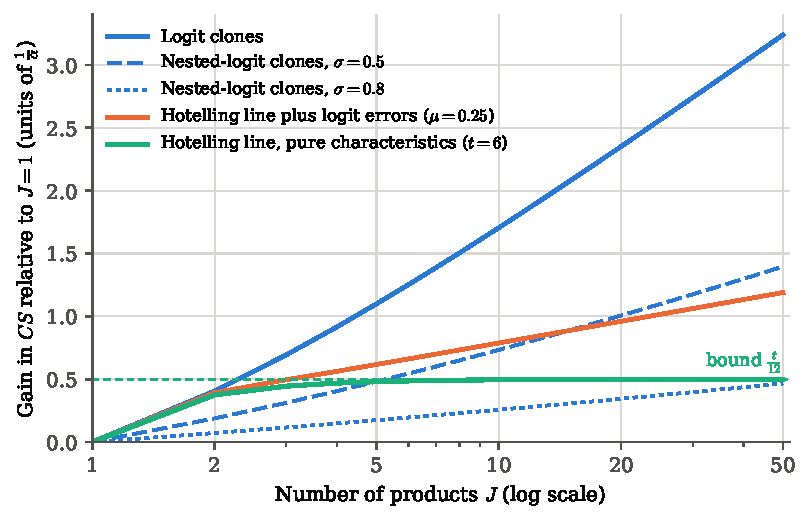
\includegraphics[width=0.88\textwidth]{figures/ch10/variety_value.pdf}
\caption{Gain in consumer surplus from adding products, relative to a market with one product, in units of
$\frac{1}{\alpha}$. The logit and nested-logit curves add identical products with $\delta = 0$ in the presence of
an outside good. The Hotelling curves place $J$ products evenly on a line with uniform consumers, quadratic
transport cost $t = 6$ and fixed equal prices. The orange curve adds logit errors with scale $\mu = 0.25$ to the
Hotelling model. At $J = 50$ the gains are 3.24 (logit), 1.40 and 0.47 (nested logit with $\sigma = 0.5$ and
$0.8$), 1.19 (Hotelling with errors) and 0.50 (pure Hotelling). Only the models with idiosyncratic errors grow
without bound. For the Hotelling curves we set $\alpha = 1$, so all curves are in the same units. Our
computations.}
\label{fig:10-variety-value}
\end{figure}

\Citet{AckerbergRysman2005} propose a correction within the logit family. It lets the contribution of the
idiosyncratic term depend on how crowded the product space is, so that additional products add less.

\subsection{Pure characteristics and vertical models}\label{sec:10-cs-pure}

\Citet{BerryPakes2007} develop the pure characteristics model for empirical work. Their utility is
\begin{equation}\label{eq:10-bp-utility}
u_{ij} = x_j\beta_i - \alpha_ip_j + \xi_j,
\qquad u_{i0} = 0,
\end{equation}
with random coefficients $\beta_{ik} = \beta_k + \sigma_k\nu_{ik}$ and $\alpha_i > 0$, after normalizing the
coefficient on the single unobserved characteristic $\xi_j$ to one. The model has no $\epsilon_{ij}$. They show
that the two families of models differ in two respects (pp.~2--3 and 6--7 of their text). With tastes for products,
substitution between products is limited and markups stay bounded away from zero as similar products are added.
Each consumer's utility also grows without bound as products are added, whatever their characteristics. In the
pure characteristics model, the gain from a new product is limited by a smooth function of its distance from
existing products. As the space fills, products become close substitutes, prices approach marginal cost, and the
increment in welfare from each new product declines to zero.

The $\epsilon$'s have practical advantages, which explain their popularity. They make choice probabilities
integrals with simple limits, and they keep every probability positive with smooth derivatives. They also allow the
share inversion that turns $\xi_j$ into a linear function of data and parameters
\citep{Berry1994,BerryLevinsohnPakes1995}.
Without them the share function has kinks and the inversion is no longer a contraction. Berry and Pakes therefore
propose to use the vertical model of \cref{ch:discrete} for the price coefficient, conditional on the other
coefficients, and a homotopy method to compute the mean utilities. A \emph{homotopy method} solves a hard system
of equations by deforming an easy system into it and following the solution path. They also study a ``modified BLP'' model in
which the logit term is scaled by $\frac{1}{\mu_\epsilon}$. The pure characteristics model is the limit as
$\mu_\epsilon\to\infty$.

\casehead{Welfare in a Monte Carlo experiment} The last experiment in \citet[Section 5.4]{BerryPakes2007} speaks to
new goods. The data come from a pure characteristics model with three markets, structured as successive years of
a market with improving characteristics. The number of products rises from 75 to 100 and then to 125. The
characteristics are patterned on the megahertz of personal computers in 1995--97 \citep{Pakes2003}, and prices for
given characteristics fall by roughly 30 percent a year. The welfare measure is the average gain per person, in
dollars, from moving from the year-one choice set to the year-three choice set. \Cref{tab:10-bp-welfare} reports
it.

\begin{table}[htbp]
\centering
\caption{Welfare gain from the year-one to the year-three choice set in the Berry-Pakes Monte Carlo}
\label{tab:10-bp-welfare}
\small
\begin{tabular}{@{}lr@{}}
\toprule
Method & Gain \\
\midrule
True (pure characteristics data-generating process) & 266.1 \\
Homotopy estimator of the pure characteristics model & 265.3 \\
Modified BLP, scale fixed at $\mu_\epsilon = 10$ & 270.0 \\
Modified BLP, scale $\mu_\epsilon$ estimated & 259.0 \\
Modified BLP, $\mu_\epsilon$ estimated, final homotopy contraction & 272.1 \\
\bottomrule
\end{tabular}

\smallskip
\begin{minipage}{0.86\linewidth}
\footnotesize Notes: Average per-person gain in dollars. One simulated data set with an average of 100 products per
market. The estimated scale in the fourth row is 0.934 with standard error 6.680, and the estimated constant in
mean utility is $-6.455$ against a true value of 2. Source: \citet{BerryPakes2007}, Tables 5 and 7.
\end{minipage}
\end{table}

All methods come within 3 percent of the truth. The modified BLP estimator with estimated scale does badly on
parameters and elasticities. For the lowest-priced product its own-price elasticity is $-1.8$ against a true
$-11.0$ \citep[Table 6]{BerryPakes2007}. Yet its welfare gain is close to the truth. Berry and Pakes explain why.
Because the contraction fits the shares exactly, the extra gain from the logit errors is offset by lower mean
utilities $\delta$, and the two roughly cancel. The estimated constant in $\delta$ falls below $-6$ to match the
small shares with a large logit error. The lesson is double-edged. Fitting shares exactly protects welfare
measures against part of the $\epsilon$ problem in this design, but it does so by distorting the parameters that
govern substitution.

\casehead{The hedonic approach} \Citet{BajariBenkard2005} take a different route to demand without
$\epsilon_{ij}$. Their method has two stages in the spirit of \citet{Rosen1974}. The first estimates a hedonic
price function $p_j = \mathbf{p}(x_j,\xi_j)$ that allows one unobserved characteristic and a non-additive form, and
recovers the $\xi_j$. They show that a hedonic price surface exists even with imperfect competition and finitely
many products. The second stage recovers tastes from each consumer's first-order conditions. At the chosen
product, the marginal utility of each continuous characteristic equals the marginal utility of money times the
slope of the price surface,
\begin{equation}\label{eq:10-bb-foc}
\frac{\partial u_i}{\partial x_{jk}} = \alpha_i\,\frac{\partial\mathbf{p}}{\partial x_{jk}} .
\end{equation}
With a continuum of products this inverts to each consumer's taste vector. With finitely many products the
revealed-preference conditions place each consumer's tastes in a set, which shrinks as the number of products
grows. The unobserved characteristic is essential. In their data on personal computers, 357 of 695 products are
dominated by another product that is better in every observed dimension and cheaper
\citep[p.~2]{BenkardBajari2004}.
They also note that the $\epsilon_{ij}$ amount to assuming an infinite-dimensional characteristics space, and that
logit-type demand curves typically are hyperbolic, approaching both axes. The hedonic model imposes no shape
beyond a downward slope, so the two families can predict quite different demand at prices outside the observed
range. That range is exactly where new-good valuations live.

\casehead{A vertical example} The vertical model of \cref{ch:discrete} makes the role of distance transparent.
Utility is $U_{ij} = \delta_j - \nu_ip_j$, with $\nu_i > 0$ distributed with continuous density $f$ on
$(0,\infty)$. A consumer's marginal utility of money is $\nu_i$, so a utility gain $\Delta U$ is worth
$\frac{\Delta U}{\nu_i}$ dollars to her. Products that sell are ordered by price and quality, and consumer $i$ buys
$j$ when $\nu_i$ lies between the cutoffs $c_{j,j+1} = \frac{\delta_{j+1}-\delta_j}{p_{j+1}-p_j}$ and $c_{j-1,j}$.

\begin{proposition}[Value of a new product in the vertical model]\label{prop:10-vertical-gain}
Let $j$ and $j+1$ be adjacent products with positive shares, $p_j < p_{j+1}$, and $c^* = c_{j,j+1} > 0$. Insert
product $n$ with $p_j < p_n < p_{j+1}$ and quality
\begin{equation}\label{eq:10-vertical-d}
\delta_n = \delta_j + c^*(p_n - p_j) + d ,
\end{equation}
so that $d$ is the vertical distance of the point $(p_n,\delta_n)$ above the chord joining $(p_j,\delta_j)$ and
$(p_{j+1},\delta_{j+1})$. Hold all other prices fixed, and take $d$ small enough that the new cutoffs stay inside
$(c_{j+1,j+2},\,c_{j-1,j})$.
\begin{enumerate}[label=(\alph*)]
\item If $d\le 0$, product $n$ sells nothing and creates no surplus.
\item If $d > 0$, exactly the consumers with $\nu\in(\nu_L,\nu_H)$ switch to $n$, where
\begin{equation*}
\nu_L = c^* - \frac{d}{p_{j+1} - p_n},
\qquad
\nu_H = c^* + \frac{d}{p_n - p_j}.
\end{equation*}
\item The money-metric gain of consumer $\nu$ is $g(\nu) = \frac{1}{\nu}\left[U_n(\nu) - \max\{U_j(\nu),
U_{j+1}(\nu)\}\right]^+$. It is positive on $(\nu_L,\nu_H)$ and equals $\frac{d}{c^*}$ at $\nu = c^*$.
\item The total gain $\mathcal{G} = \int g(\nu)f(\nu)\,d\nu$ satisfies the first expansion below. If in addition
$f(c^*) > 0$, the share $s_n$ is first order in $d$ and the gain per buyer satisfies the second,
\begin{equation}\label{eq:10-vertical-gain}
\mathcal{G} = \frac{f(c^*)}{2c^*}\,\frac{p_{j+1} - p_j}{(p_n - p_j)(p_{j+1} - p_n)}\,d^2 + o(d^2),
\qquad
\frac{\mathcal{G}}{s_n} = \frac{d}{2c^*} + o(d).
\end{equation}
\end{enumerate}
\end{proposition}

\begin{proof}
At $\nu = c^*$ the old products give equal utility, $U_j(c^*) = U_{j+1}(c^*)$. Using \eqref{eq:10-vertical-d},
\begin{equation*}
U_n(c^*) - U_j(c^*) = \delta_n - \delta_j - c^*(p_n - p_j) = d .
\end{equation*}
For $\nu > c^*$ the relevant rival is $j$, and $U_n(\nu) - U_j(\nu) = d - (\nu - c^*)(p_n - p_j)$. This difference
vanishes at $\nu_H$. For $\nu < c^*$ the rival is $j+1$, and $U_n(\nu) - U_{j+1}(\nu) = d + (c^* - \nu)(p_n -
p_{j+1})$, which vanishes at $\nu_L$. Both differences are linear in $\nu$ with peak $d$ at $c^*$.

(a) If $d \le 0$, $U_n(\nu) \le \max\{U_j(\nu),U_{j+1}(\nu)\}$ for every $\nu$, by the two linear expressions. No
consumer strictly prefers $n$.

(b) and (c) For $d > 0$, $n$ beats the better of $j$ and $j+1$ exactly on $(\nu_L,\nu_H)$. The bound on $d$
ensures that products other than $j$ and $j+1$ remain worse for these consumers. Dividing the utility gain by
$\nu$ gives $g(\nu)$, which equals $\frac{d}{c^*}$ at $c^*$.

(d) Let $h(\nu) = \nu g(\nu)$ denote the utility gain. It is a triangle with height $d$ and base $\nu_H - \nu_L$,
where
\begin{equation*}
\nu_H - \nu_L = d\left(\frac{1}{p_n - p_j} + \frac{1}{p_{j+1} - p_n}\right)
= d\,\frac{p_{j+1} - p_j}{(p_n - p_j)(p_{j+1} - p_n)} .
\end{equation*}
Its area is $\frac{1}{2}d(\nu_H - \nu_L)$. Since $\frac{f(\nu)}{\nu}$ is continuous at $c^* > 0$ and the interval
shrinks to $c^*$, $\frac{f(\nu)}{\nu} = \frac{f(c^*)}{c^*} + o(1)$ uniformly on it. Therefore
\begin{equation*}
\mathcal{G} = \int_{\nu_L}^{\nu_H}h(\nu)\frac{f(\nu)}{\nu}\,d\nu
= \left(\frac{f(c^*)}{c^*} + o(1)\right)\frac{d}{2}(\nu_H - \nu_L),
\end{equation*}
which is the first part of \eqref{eq:10-vertical-gain}. This step holds also when $f(c^*) = 0$, and the
coefficient on $d^2$ is then zero. The share is $s_n = F(\nu_H) - F(\nu_L) = (f(c^*) + o(1))(\nu_H - \nu_L)$.
When $f(c^*) > 0$, the factor $f(c^*) + o(1)$ is bounded away from zero for small $d$. Dividing the two
expressions then gives $\frac{\mathcal{G}}{s_n} = \frac{d}{2c^*} + o(d)$.
\end{proof}

The condition $f(c^*) > 0$ matters for the per-buyer formula. Take the density $f(\nu) = (\nu - 1)^2e^{-\nu}$,
old products $(p,\delta) = (1,2)$ and $(3,4)$, an outside utility of zero and the new product $(2,3+d)$. Then
$c^* = 1$ and $f(c^*) = 0$. Our computation gives $s_n = \frac{2e^{-1}d^3}{3} + o(d^3)$ and
$\mathcal{G} = \frac{e^{-1}d^4}{6} + o(d^4)$, so that $\frac{\mathcal{G}}{s_n} = \frac{d}{4} + o(d)$. This is half
the value $\frac{d}{2c^*} = \frac{d}{2}$ of \eqref{eq:10-vertical-gain}.

\Cref{fig:10-vertical-gain} draws the construction. When $f(c^*) > 0$, the gain is second order in the
distance $d$. The share of the new product is then first order in $d$, and the gain per buyer, $\frac{d}{2c^*}$,
vanishes as the new product approaches the chord. The quantity $\frac{d}{c^*}$ is the dollar value of the new product's quality premium at the margin
between its neighbors, and the average switcher gets half of it, as in any triangle. Compare
\eqref{eq:10-logit-perbuyer}. In the logit the gain per buyer is at least $\frac{1}{\alpha}$ for any product,
including a product on or below the chord. A numerical check with $f(\nu) = e^{-\nu}$ and the prices of
\cref{fig:10-vertical-gain} confirms \eqref{eq:10-vertical-gain}. The exact gain differs from the approximation by
1.7 percent at $d = 0.2$ and by 0.1 percent at $d = 0.05$.

\begin{figure}[htbp]
\centering
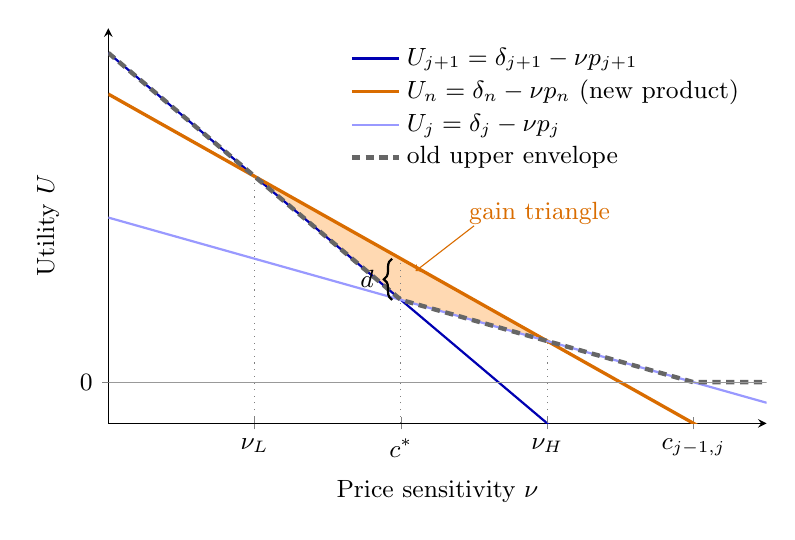
\begin{tikzpicture}
\begin{axis}[
  width=0.82\textwidth, height=6.6cm,
  xmin=0, xmax=2.25, ymin=-0.5, ymax=4.3,
  axis lines=left, clip=true,
  xlabel={Price sensitivity $\nu$}, ylabel={Utility $U$},
  xtick={0.5,1,1.5,2}, xticklabels={$\nu_L$,$c^*$,$\nu_H$,$c_{j-1,j}$},
  ytick={0}, yticklabels={$0$},
  every axis x label/.style={at={(axis description cs:0.5,-0.12)},anchor=north},
  every axis y label/.style={at={(axis description cs:-0.06,0.5)},rotate=90,anchor=south},
  tick label style={font=\small}, label style={font=\small},
  legend style={at={(0.98,0.98)}, anchor=north east, draw=none, fill=white, font=\small},
  legend cell align=left]
  \fill[orange!30] (axis cs:0.5,2.5) -- (axis cs:1,1) -- (axis cs:1.5,0.5) -- cycle;
  \addplot[blue!70!black, thick, domain=0:2.25, samples=2] {4 - 3*x};
  \addlegendentry{$U_{j+1} = \delta_{j+1} - \nu p_{j+1}$}
  \addplot[orange!85!black, very thick, domain=0:2.25, samples=2] {3.5 - 2*x};
  \addlegendentry{$U_n = \delta_n - \nu p_n$ (new product)}
  \addplot[blue!40, thick, domain=0:2.25, samples=2] {2 - x};
  \addlegendentry{$U_j = \delta_j - \nu p_j$}
  \addplot[black!60, densely dashed, line width=1.6pt] coordinates {(0,4) (1,1) (2,0) (2.25,0)};
  \addlegendentry{old upper envelope}
  \draw[black!50, dotted] (axis cs:0.5,-0.5) -- (axis cs:0.5,2.5);
  \draw[black!50, dotted] (axis cs:1,-0.5) -- (axis cs:1,1.5);
  \draw[black!50, dotted] (axis cs:1.5,-0.5) -- (axis cs:1.5,0.5);
  \draw[black!40] (axis cs:0,0) -- (axis cs:2.25,0);
  \draw[decorate, decoration={brace, amplitude=3pt}, thick] (axis cs:0.97,1.0) -- (axis cs:0.97,1.5)
     node[midway, left=3pt, font=\small] {$d$};
  \node[font=\small, orange!85!black, anchor=west] at (axis cs:1.2,2.05) {gain triangle};
  \draw[->, orange!85!black] (axis cs:1.25,1.9) -- (axis cs:1.05,1.35);
\end{axis}
\end{tikzpicture}
\caption{The vertical model with a product inserted between two neighbors. Each line is the utility $\delta - \nu p$
of one product as a function of price sensitivity $\nu$. The dashed line is the upper envelope before the
introduction, and the outside good gives utility zero. Product $n$ lies a distance $d$ above the chord joining its
neighbors and wins the consumers with $\nu\in(\nu_L,\nu_H)$. The shaded triangle is their utility gain, so the
welfare gain is of order $d^2$. The parameters are $(p_j,p_n,p_{j+1}) = (1,2,3)$ and $(\delta_j,\delta_n,\delta_{j+1}) =
(2,3.5,4)$, so $c^* = 1$ and $d = 0.5$.}
\label{fig:10-vertical-gain}
\end{figure}

\subsection{Hedonic methods, quality change and changing tastes}\label{sec:10-cs-hedonic}

Statistical agencies often handle new varieties with hedonic methods, and the vertical example shows what these
methods assume. A \emph{hedonic price function} $\mathbf{p}(z)$ relates the prices of products to their
characteristics $z$ \citep{Griliches1971,Rosen1974}. We write
\begin{equation}\label{eq:10-hedonic}
p_j = \mathbf{p}(z_j) + \tilde p_j ,
\end{equation}
where $\tilde p_j$ is the \emph{residual price}, the deviation of product $j$'s price from the surface. In Rosen's
model with a continuum of products, the hedonic function is an equilibrium locus. A consumer with utility
$\alpha[y - \mathbf{p}(z)] + \phi(z)$ chooses $z$ to satisfy $\mathbf{p}'(z) = \frac{\phi'(z)}{\alpha}$. A new
variety priced on the surface offers nothing that consumers could not already buy, so it adds no surplus. Hedonic
quality adjustment therefore treats a new variety as a perfect substitute for a combination of existing ones.
This is the flat curve $dd(-\infty)$ of \cref{fig:10-dd-DD}, which \citet[p.~238]{Bresnahan1997} identifies as an
understatement of the value of new goods. In the vertical model the chord between neighbors plays the role of the
hedonic surface. A product priced on it has $d = 0$ and adds nothing, while a product above it adds a gain of
order $d^2$. When the product space is sparse, the surface has wide gaps and the understatement can be large.

\casehead{Quality as repackaging} \citet[Section~10.3, pp.~262--266]{DeatonMuellbauer1980b} derive the most common
hedonic regression from a model in which quality repackages quantity. The varieties $j$ of a good are perfect
substitutes once each is weighted by a quality index $\zeta_j > 0$. Utility is
$v\bigl(h(\sum_j\zeta_jq_j),q_{\mathrm{other}}\bigr)$, where $q_{\mathrm{other}}$ collects the other goods (their
eq.~3.7). A consumer then buys only the varieties with the lowest price per unit of quality,
$\frac{p_{jt}}{\zeta_j}$. Suppose all consumers share the weights and every variety sells. The prices per unit of
quality must then be equal, $p_{jt} = \zeta_jP_t$, where $P_t$ is the price of a unit of quality in period $t$. With
$\ln\zeta_j = f(z_j)$, taking logs gives
\begin{equation}\label{eq:10-dm-hedonic}
  \ln p_{jt} = \ln P_t + f(z_j)
\end{equation}
(their eq.~3.8). A disturbance and a log-linear $f$ give the \emph{time-dummy hedonic regression}. It pools all periods
and adds a zero-one dummy for each period except a reference period (p.~263). The coefficients on the
period dummies estimate $\ln P_t$, a quality-corrected price index. A new variety priced on this surface sells
quality at the going price $P_t$, so it adds no surplus. Their Table~10.1 (p.~264) fits such a regression to 150
British used-car models, aged one to three years, from nine manufacturers in the late 1950s and the 1960s. A 1
percent increase in brake horsepower raises the price by 0.370 percent (standard error 0.023). The implied
quality-corrected price of cars was about 8 percent lower in 1969 than in 1958 (p.~263). The coefficients on miles
per gallon, $-0.064$ (0.041), and interior size, $-0.146$ (0.094), are negative and imprecise. Deaton and Muellbauer
suggest that, with length and width held fixed, a large interior may signal restricted luggage space (p.~264).
An $F$-test rejects a common price function across manufacturers. The statistic is 9, and 1.2 suffices to reject at
the 5 percent level (p.~265). Deaton and Muellbauer read this as evidence of \emph{market segmentation}, in which
products made for different types of consumers carry different shadow prices of characteristics (p.~259). A single
price surface ignores it. When consumers' weights differ, the surface is instead an envelope of their
\emph{bid functions}. A consumer's bid function gives the most she would pay for one unit of a variety with
characteristics $z$, at her utility level (pp.~265--266). The marginal condition
$\frac{\partial\ln\mathbf{p}(z)}{\partial z_k} = \frac{\partial\ln\zeta(z)}{\partial z_k}$ then holds for each
consumer at her chosen variety, as in \citet{Rosen1974} (eq.~3.10, pp.~265--266).

\casehead{Changing tastes: ex ante and ex post measures} Applications over long periods face a further problem.
If the estimated taste parameters change from year to year, the value of moving from choice set $S_t$ to $S_{t+1}$
depends on which year's tastes are used. Write $\mathcal{W}^t$ for the surplus function evaluated with the
parameters estimated for year $t$. \citet[pp.~56--58]{Trajtenberg1985} defines
\begin{equation}\label{eq:10-exante-expost}
\Delta\mathcal{W}^a = \mathcal{W}^t(S_{t+1}) - \mathcal{W}^t(S_t),
\qquad
\Delta\mathcal{W}^p = \mathcal{W}^{t+1}(S_{t+1}) - \mathcal{W}^{t+1}(S_t).
\end{equation}
The \emph{ex ante} measure $\Delta\mathcal{W}^a$ asks what a consumer with today's tastes would pay to face next
year's choice set. The \emph{ex post} measure $\Delta\mathcal{W}^p$ asks how much income could be taken from a
consumer with next year's tastes, leaving her indifferent between next year's and this year's sets. The
distinction resembles the one between compensating and equivalent variation, but it has a different source.
Compensating and equivalent variation hold tastes fixed and differ in the reference utility level, and they
coincide without income effects. Here utility is quasi-linear, and the ambiguity comes from the change in the taste
parameters themselves. The hybrid $\mathcal{W}^{t+1}(S_{t+1}) - \mathcal{W}^t(S_t)$ compares utilities under two
different preference structures, which is an interpersonal comparison and has no welfare meaning.

Trajtenberg expects the ex ante measure to exceed the ex post one. His argument is a \emph{dual inducement}
mechanism. Strong tastes for an attribute induce firms to improve that attribute, and the improvement then lowers
its marginal valuation next year. Judged by the original tastes, an improvement is therefore worth more. He also
considers a Divisia-like alternative that estimates adjacent years jointly. It yields a unique measure, but only by
suppressing the taste differences that create the problem.

\section{Case study: CT scanners (Trajtenberg 1989)}\label{sec:10-trajtenberg}

\citet{Trajtenberg1989} was the first study to measure a product innovation by the welfare it creates, using an
estimated discrete-choice demand system in characteristics space. The application is computed tomography (CT)
scanners in the United States from their introduction in 1973 to 1982. The paper is also an early study of how
innovation, diffusion and returns to research interact. The PDF available to us is the working-paper version
\citep{Trajtenberg1985}. All numbers below come from it, and page numbers refer to its typed pages. The
published version may number its tables differently, and some of its numbers may differ.
Trajtenberg indexes products by $i$ and characteristics by $j$. We index scanners by $j$ and characteristics by
$k$, consistent with the rest of the book.

\subsection{The question}\label{sec:10-ct-question}

The output of innovative activity does not come in countable units. Patent counts vary enormously in
significance, and sales of new products confound innovation with market size. Trajtenberg therefore argues that a
quantitative measure of innovation can only be defined in value terms
\citep[pp.~2--3]{Trajtenberg1985}. How much product innovation occurred in a field over a period is the
additional social surplus that the innovations generated. Other measures can at best serve as proxies.

A product is a pair $(z_j,p_j)$, with $z_j = (z_{j1},\dots,z_{jK})$ its characteristics and $p_j$ its price.
Trajtenberg writes $s_j$ for this pair, a symbol we keep for market shares.
The choice set in year $t$ is $S_t$, and product innovation is the change $S_t - S_{t-1}$. It includes improvements
in existing products, the addition of new ones and the exit of old ones. The magnitude of innovation is
\begin{equation}\label{eq:10-traj-dW}
\Delta\mathcal{W}_t = \mathcal{W}(S_t) - \mathcal{W}(S_{t-1}),
\end{equation}
for a surplus function $\mathcal{W}$ (equation 1 of the paper, p.~7). The measure includes the effect of price
changes. Trajtenberg defends this broad definition on practical grounds. With nonlinear surplus functions the
effects of characteristics and prices cannot be separated, and new products have no earlier price to compare with
(pp.~8--9).

What counts as a product innovation needs a definition, and Trajtenberg provides one through the nature of
characteristics (pp.~4--6).

\begin{definition}[Concatenable characteristics]\label{def:10-concatenable}
Let $x_j$ be the quantity of product $j$ that a consumer buys. Characteristic $k$ is \emph{concatenable} if the
amount of it available to the consumer is $z_{jk} = f^k(x_j)$ with $\frac{\partial z_{jk}}{\partial x_j} \ne 0$.
Examples are the protein in a food or the carrying capacity of vehicles. It is \emph{non-concatenable} if
$z_{jk} = g^k(\theta_j)$ for the product's natural unit $\theta_j$, with $\frac{\partial z_{jk}}{\partial x_j} = 0$
for $x_j > \theta_j$. Examples are the speed of a vehicle or the aperture of a camera.
\end{definition}

Product innovation requires at least one non-concatenable characteristic. Suppose all characteristics were
concatenable and linear in quantity. Then a change from $(z_j,p_j)$ to $(\kappa z_j,\kappa p_j)$ with
$\kappa > 1$ would leave the indirect utility unchanged, $V(z_j,p_j,y) = V(\kappa z_j,\kappa p_j,y)$. Buying $\kappa$ units of the old
product delivers the same bundle at the same cost. Such a change could not count as an innovation. A product
innovation therefore presupposes a quality dimension that can be changed only by switching products. CT scanners
satisfy this. Speed and image resolution are properties of the machine. Buying more machines does not change
them.

\casehead{Scope} The surplus function is in principle total surplus. Trajtenberg argues that profits pose no
special measurement problem beyond accounting, so the difficulty lies in consumer surplus. He measures the gains
that are not appropriated by the innovating firms and passed on to buyers (pp.~9--10). He states two limitations.
Radical innovations, which open new product classes, cannot be measured directly (\cref{sec:10-cs-predict}). The
measure also ignores spillovers to other product classes, so it is a lower bound on the social gain (pp.~11--12).
Trajtenberg proposes an indirect estimate of the gain from the first scanner, based on diffusion
(\cref{sec:10-ct-diffusion}).

The question matters for three reasons. Product innovation is a large part of technical change, and official
price and productivity statistics do not capture it (p.~1). Social returns to research cannot be computed without
a measure of benefits. And the interaction between innovation and diffusion cannot be studied without a measure of
innovation.

\subsection{Setting}\label{sec:10-ct-setting}

Research on computed tomography began in 1967 at the British electronics company EMI. The first operational
prototype was installed in a London hospital in 1971, and the first commercial system, the EMI Scanner, was
installed in the United States in June 1973 (p.~25). In 1974--77 nearly 20 firms entered. They ranged from
electronics companies (General Electric, Siemens, Hitachi, Philips) to pharmaceutical companies (Pfizer, Searle,
Syntex) and specialized firms (AS\&E, Elscint), and they competed mainly through product performance (p.~26).
Diffusion among U.S. hospitals was fast, the fifth fastest among twenty innovations for which diffusion studies
existed (p.~26, n.~23). Mounting concern about health-care costs led to Certificate of Need regulation, which
required approval for large hospital investments. Its full impact in 1978--79 produced a sharp downturn and the
exit of many firms, including EMI. The market then recovered and settled at 10--15 percent annual growth, with
General Electric holding about 50 percent of the U.S. market and some ten firms sharing the rest (p.~26). The two
pioneers of CT received the Nobel Prize in Medicine in 1979.

\casehead{Characteristics} A CT scanner takes cross-sectional images of the body. Trajtenberg measures three
performance characteristics (pp.~27--30). SPEED is the minimum scan time in seconds. The first scanner took five
minutes per scan, which restricted it to the brain, a motion-free organ. Scan times of twenty seconds and less
opened other organs, and the fastest systems of the early 1980s scanned in about one second. RESOL is spatial
resolution in millimeters, the size of the smallest object visible in high-contrast regions. Trajtenberg had
constructed a fuller image-quality index from experimental data, but it was unavailable for most of the roughly
50 systems marketed. RTIME is reconstruction time in seconds, the time the computer takes to produce the image. A
fourth attribute, gantry tilt, proved insignificant and was dropped. All three characteristics are defined so that
less is better. Scanners come in two types. \emph{Head scanners} can image only the brain, while \emph{body
scanners} can image almost any organ.

\subsection{Data}\label{sec:10-ct-data}

Trajtenberg assembled his own data bank, covering the period from the announcement of the innovation in 1972 to
1981, with some series extending to 1983 (pp.~30--32). It has four parts. The first gives the technical
characteristics and prices of all CT scanners marketed up to 1982, by year, which is the sequence of choice sets
$S_t$. The second records every installation in the United States, with the identity of the hospital or clinic,
the dates of order and installation, and the model bought. It has more than 2,000 observations, including
upgrades, and Trajtenberg estimates that it covers about 98 percent of U.S. installations up to July 1981. The
third describes the hospitals and the fourth the manufacturers, including their research and development spending
on CT. The main source is a questionnaire to all manufacturers, with follow-up contacts. Others are the radiology
and medical-physics literature, trade journals and consulting reports. Public sources include the Food and Drug
Administration, the Office of Technology Assessment, the Patent Office and the American Hospital Association, and
Trajtenberg also ran a telephone survey of hospitals.
All but two firms active in 1981 answered the questionnaire. The two were CGR and Philips, and Philips was excluded
for lack of reliable information. Little is lost, since it had sold fewer than twenty scanners in the United States by
1981.

A year in the data runs from November 1 of the previous year to October 31. Most new scanners are introduced at
the annual meeting of the Radiological Society of North America in November, so this \emph{radiological year}
matches the timing of choice sets. Data for 1981 cover only the first half of that year (p.~33, n.~28).
\Cref{tab:10-ct-data} reproduces Tables 1 and 2 of the paper.

\begin{table}[htbp]
\centering
\caption{CT scanners in the United States, 1973--1982}
\label{tab:10-ct-data}
\footnotesize
\setlength{\tabcolsep}{4.5pt}
\begin{tabular}{@{}lrrrrrrrr@{}}
\toprule
\multicolumn{9}{@{}l}{\textit{Panel A. Prices and average characteristics}} \\
& \multicolumn{2}{c}{Price (\$K)} & \multicolumn{2}{c}{SPEED (s)} & \multicolumn{2}{c}{RESOL (mm)} &
  \multicolumn{2}{c}{RTIME (s)} \\
\cmidrule(lr){2-3}\cmidrule(lr){4-5}\cmidrule(lr){6-7}\cmidrule(lr){8-9}
Year & Head & Body & Head & Body & Head & Body & Head & Body \\
\midrule
1973 & 310 & -- & 300 & -- & 3.1 & -- & 300 & -- \\
1974 & 370 & -- & 300 & -- & 1.7 & -- & 30 & -- \\
1975 & 379 & 365 & 285 & 195.0 & 1.8 & 1.6 & 20 & 8 \\
1976 & 374 & 471 & 105 & 63.0 & 1.7 & 1.5 & 60 & 83 \\
1977 & 354 & 573 & 95 & 19.0 & 1.7 & 1.3 & 54 & 38 \\
1978 & 167 & 620 & 96 & 7.1 & 1.6 & 1.2 & 29 & 30 \\
1979 & 154 & 667 & 150 & 6.6 & 1.5 & 1.1 & 19 & 29 \\
1980 & 154 & 739 & 115 & 5.5 & 1.5 & 1.0 & 27 & 31 \\
1981 & 150 & 827 & 115 & 4.9 & 1.5 & 0.8 & 27 & 32 \\
1982 & 150 & 850 & 115 & 2.6 & 1.5 & 0.7 & 27 & 27 \\
\midrule
\multicolumn{9}{@{}l}{\textit{Panel B. Market indicators}} \\
& Units & Sales & Body & New & Firms & Models & HHI & \\
Year & sold & (\$M) & (\% sales) & adopters (\%) & & & & \\
\midrule
1973 & 16 & 5 & 0 & 100.0 & 1 & 1 & 1.00 & \\
1974 & 74 & 27 & 0 & 98.7 & 1 & 1 & 1.00 & \\
1975 & 221 & 82 & 44.8 & 97.7 & 4 & 5 & 0.43 & \\
1976 & 374 & 167 & 76.2 & 84.8 & 9 & 14 & 0.38 & \\
1977 & 385 & 208 & 84.9 & 84.1 & 12 & 23 & 0.23 & \\
1978 & 248 & 122 & 72.4 & 84.4 & 10 & 23 & 0.28 & \\
1979 & 273 & 141 & 70.2 & 76.0 & 9 & 22 & 0.26 & \\
1980 & 270 & 169 & 80.4 & 65.3 & 8 & 17 & 0.32 & \\
1981 & 392 & 302 & 91.6 & 50.0 & 8 & 14 & 0.31 & \\
1982 & 428 & 344 & 93.5 & n.a. & 8 & 16 & 0.30 & \\
\bottomrule
\end{tabular}

\smallskip
\begin{minipage}{0.94\linewidth}
\footnotesize Notes: Radiological years (November to October), U.S. market. Price is the sales-weighted average
price of all scanners of each type. The characteristics are simple averages, and smaller values are better.
``Body'' is the share of body scanners in unit sales and ``New adopters'' the share of sales to first-time
buyers. HHI is the Herfindahl index. Source: \citet{Trajtenberg1985}, Tables 1 and 2.
\end{minipage}
\end{table}

The two types followed opposite paths (pp.~32--33). Head scanners became simpler and cheaper, and their price
fell from \$379K in 1975 to \$150K by 1981. Body scanners improved quickly, with average scan time
falling from 195 seconds in 1975 to 2.6 seconds in 1982, and their price rose from \$365K to \$850K. By most
indicators competition peaked in 1977. Fourteen new scanners were introduced that year, the number of firms
reached 12, and the Herfindahl index reached its low of 0.23. Sales to new adopters fell from 97.7 percent of
sales in 1975 to 50.0 percent in 1981 as diffusion leveled off and replacement purchases grew.

\subsection{The model}\label{sec:10-ct-model}

\casehead{Demand and the surplus function} A buyer chooses one scanner from $S$. She spends the rest of income
$y$ on a composite outside good $m$ with unit price (pp.~15--17),
\begin{equation}\label{eq:10-traj-rum}
\max_{j,m}\; U(z_j,m;D) + \epsilon_j
\qquad\text{subject to}\qquad p_j + m = y,\quad j\in S,
\end{equation}
where $D$ is a vector of buyer attributes. Substituting $m = y - p_j$ gives the conditional indirect utility
$V(z_j,y - p_j;D) + \epsilon_j$. With \iid\ type-I extreme value shocks and quasi-linear utility $\alpha(y - p_j) +
\phi(z_j;D) + \epsilon_j$, income cancels and the choice probabilities are
\begin{equation}\label{eq:10-traj-mnl}
s_j = \frac{e^{-\alpha p_j + \phi(z_j;D)}}{\sum_{k\in S}e^{-\alpha p_k + \phi(z_k;D)}},
\qquad j\in S .
\end{equation}
There is no outside good. The model describes the choice among scanners by buyers who buy one, and the decision
to adopt is modeled separately (\cref{sec:10-ct-diffusion}). By \cref{lem:10-logsum,lem:10-cv-quasilinear} the
surplus function is
\begin{equation}\label{eq:10-traj-W}
\mathcal{W}(S;D) = \frac{1}{\alpha}\ln\sum_{j\in S}e^{-\alpha p_j + \phi(z_j;D)},
\end{equation}
which is equation (10) of the paper (p.~18), and its entropy decomposition is \cref{prop:10-entropy}. Trajtenberg
notes that the surplus function treats the buyer as if she bought a fraction $s_j$ of every product. Every change in
the set therefore registers, whichever product a buyer ends up with. He rejected the probit because his choice sets
had up to twenty alternatives, and the computers of the time could handle a probit with only four or five.

\casehead{Hedonic prices and the collinearity problem} In markets for differentiated products, prices are closely
related to characteristics through the hedonic function \eqref{eq:10-hedonic}. Entering both $p_j$ and $z_j$ in
\eqref{eq:10-traj-mnl} creates severe collinearity, and their separate coefficients cannot be estimated with
precision (pp.~19--20). Trajtenberg argues that the problem is conceptual. In Rosen's continuous model the
consumer cannot choose $z$ and $p$ independently, because choosing $z$ determines $p$. With
\begin{equation}\label{eq:10-traj-rosen}
\max_{z}\; \alpha[y - \mathbf{p}(z)] + \phi(z)
\qquad\Longrightarrow\qquad
\mathbf{p}'(z) = \frac{\phi'(z)}{\alpha},
\end{equation}
only the characteristics enter the demand analysis (p.~21). In the discrete case the hedonic function is a
stochastic budget constraint. Substituting \eqref{eq:10-hedonic} into utility gives
\begin{equation}\label{eq:10-traj-netutility}
V_j = \phi(z_j) - \alpha\,\mathbf{p}(z_j) - \alpha\tilde p_j = V^n(z_j) - \alpha\tilde p_j,
\qquad
V^n(z) \equiv \phi(z) - \alpha\,\mathbf{p}(z).
\end{equation}
The term $V^n(z)$ is the \emph{net utility} of characteristics, net of their expected cost. The residual price
$\tilde p_j$ is a random extra charge or discount relative to the market's valuation of the characteristics.
Choices depend on $z_j$ and $\tilde p_j$, the part of price orthogonal to the characteristics. The next proposition
supplies the functional form for $V^n$ (p.~22).

\begin{proposition}[Quadratic approximation of net utility]\label{prop:10-quadratic}
Let $V^n$ be twice continuously differentiable with an interior point $z^*$ at which
\begin{equation*}
\frac{\partial V^n(z^*)}{\partial z_k} = \frac{\partial\phi(z^*)}{\partial z_k} - \alpha\frac{\partial\mathbf{p}(z^*)}{\partial z_k}
= 0,\qquad k = 1,\dots,K,
\end{equation*}
and let the Hessian $H = \nabla^2 V^n(z^*)$ be negative definite. Then
\begin{equation}\label{eq:10-quadratic}
V^n(z) = c_0 + z^\top\beta + z^\top Gz + o\left(\|z - z^*\|^2\right),
\qquad G = \frac{1}{2}H,\quad \beta = -Hz^*,
\end{equation}
where $c_0 = V^n(z^*) + \frac{1}{2}z^{*\top}Hz^*$ does not depend on $z$. If $\phi$ is concave and $\mathbf{p}$ is
convex near $z^*$, and $\nabla^2\phi(z^*)$ or $\nabla^2\mathbf{p}(z^*)$ is definite, then $H$ is negative definite.
\end{proposition}

\begin{proof}
A second-order Taylor expansion about $z^*$ gives
\begin{equation*}
V^n(z) = V^n(z^*) + \nabla V^n(z^*)^\top(z - z^*) + \frac{1}{2}(z - z^*)^\top H(z - z^*) + o\left(\|z - z^*\|^2\right).
\end{equation*}
The gradient term vanishes by assumption. Expanding the quadratic form with $H$ symmetric,
\begin{equation*}
\frac{1}{2}(z - z^*)^\top H(z - z^*) = \frac{1}{2}z^\top Hz - z^\top Hz^* + \frac{1}{2}z^{*\top}Hz^* .
\end{equation*}
Collecting terms gives \eqref{eq:10-quadratic}. Finally $H = \nabla^2\phi(z^*) - \alpha\nabla^2\mathbf{p}(z^*)$ is
the sum of two negative semidefinite matrices, one of which is negative definite, so $H$ is negative definite.
\end{proof}

The constant $c_0$ drops out of the logit probabilities. In a discrete market tangency is not required, and $z^*$ is
the expected optimum. Actual choices scatter around it. Products near $z^*$ are more likely to be chosen than products far
from it (p.~23). \Cref{fig:10-hedonic-net-utility} redraws the paper's Figure 1. Trajtenberg adds that $\mathbf{p}$
may be concave and the conditions still hold, provided it is less concave than $\phi$ (p.~22, n.~21). Otherwise the
expected optimum is a corner, the approximation is poor, and estimated coefficients may take the wrong signs.

\begin{figure}[htbp]
\centering
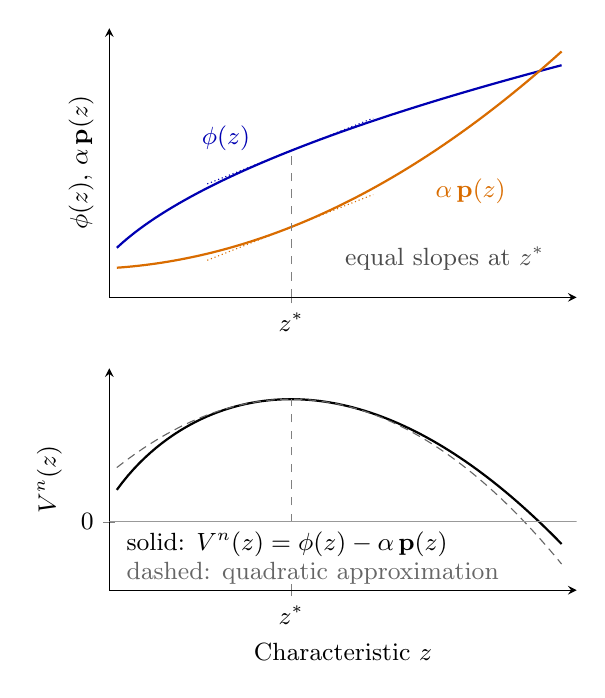
\begin{tikzpicture}
\begin{axis}[name=top,
  width=0.62\textwidth, height=5.0cm,
  xmin=0.2, xmax=3.3, ymin=0.8, ymax=4.6,
  axis lines=left, xtick={1.4057}, xticklabels={$z^*$}, ytick=\empty,
  ylabel={$\phi(z)$, $\alpha\,\mathbf{p}(z)$},
  tick label style={font=\small}, label style={font=\small}]
  \addplot[blue!70!black, thick, domain=0.25:3.2, samples=80] {2*sqrt(x) + 0.5};
  \addplot[orange!85!black, thick, domain=0.25:3.2, samples=80] {0.3*x^2 + 1.2};
  \addplot[blue!70!black, densely dotted, domain=0.85:1.95, samples=2] {2.8713 + 0.8433*(x - 1.4057)};
  \addplot[orange!85!black, densely dotted, domain=0.85:1.95, samples=2] {1.7928 + 0.8433*(x - 1.4057)};
  \draw[black!50, dashed] (axis cs:1.4057,0.8) -- (axis cs:1.4057,2.8713);
  \node[font=\small, blue!70!black, anchor=west] at (axis cs:0.75,3.05) {$\phi(z)$};
  \node[font=\small, orange!85!black, anchor=west] at (axis cs:2.3,2.3) {$\alpha\,\mathbf{p}(z)$};
  \node[font=\small, black!70, anchor=west, align=left] at (axis cs:1.7,1.35) {equal slopes at $z^*$};
\end{axis}
\begin{axis}[at={(top.south west)}, anchor=north west, yshift=-0.9cm,
  width=0.62\textwidth, height=4.4cm,
  xmin=0.2, xmax=3.3, ymin=-0.6, ymax=1.35,
  axis lines=left, xtick={1.4057}, xticklabels={$z^*$}, ytick={0}, yticklabels={$0$},
  xlabel={Characteristic $z$}, ylabel={$V^n(z)$},
  tick label style={font=\small}, label style={font=\small}]
  \addplot[black, thick, domain=0.25:3.2, samples=80] {2*sqrt(x) + 0.5 - 0.3*x^2 - 1.2};
  \addplot[black!60, densely dashed, domain=0.25:3.2, samples=80] {1.0784 - 0.45*(x - 1.4057)^2};
  \draw[black!50, dashed] (axis cs:1.4057,0) -- (axis cs:1.4057,1.0784);
  \draw[black!40] (axis cs:0.2,0) -- (axis cs:3.3,0);
  \node[font=\small, anchor=west] at (axis cs:0.25,-0.2) {solid: $V^n(z) = \phi(z) - \alpha\,\mathbf{p}(z)$};
  \node[font=\small, black!60, anchor=west] at (axis cs:0.25,-0.45) {dashed: quadratic approximation};
\end{axis}
\end{tikzpicture}
\caption{Net utility and its quadratic approximation. The top panel shows a concave utility of characteristics
$\phi(z)$ and a convex hedonic cost $\alpha\,\mathbf{p}(z)$, with equal slopes at the expected optimum $z^*$. The
bottom panel shows that net utility $V^n(z) = \phi(z) - \alpha\,\mathbf{p}(z)$ has an interior maximum at $z^*$. Its
dashed curve is the second-order expansion of \cref{prop:10-quadratic}. Illustrative functions $\phi(z) = 2\sqrt{z} + 0.5$ and
$\alpha\,\mathbf{p}(z) = 0.3z^2 + 1.2$. Redrawn after \citet{Trajtenberg1985}, Figure 1.}
\label{fig:10-hedonic-net-utility}
\end{figure}

\casehead{The separable specification} Trajtenberg simplifies further (p.~38). Suppose utility is additively
separable in characteristics, $\phi(z) = \sum_k f^k(z_k)$ with each $f^k$ quasi-concave, and the hedonic function
is linear in logs, $\mathbf{p}(z) = h_0 + \sum_k h_k\ln z_k$. Then net utility is separable too,
\begin{equation}\label{eq:10-traj-separable}
V^n(z) = \sum_k\left[f^k(z_k) - \alpha h_k\ln z_k\right] - \alpha h_0
\approx \sum_k\left(\beta_kz_k + \gamma_kz_k^2\right) + \text{const},
\end{equation}
because the Hessian of a separable function is diagonal and the cross terms of \eqref{eq:10-quadratic} vanish. The
saving of $\frac{K(K-1)}{2}$ parameters matters here. A multinomial logit (MNL) with characteristics that vary only
across products, and not across buyers, can include at most $|S| - 1$ such variables. Here $|S|$ is the number of
alternatives in the choice set $S$ (p.~38, n.~36). The separability of the hedonic function in $\ln z_k$ is what licenses the simplification. A double-log or
semi-log hedonic function would reintroduce cross terms (p.~39, n.~36).

\casehead{The estimating equation} Combining \eqref{eq:10-traj-netutility} and \eqref{eq:10-traj-separable}, the
model estimated for each year is
\begin{equation}\label{eq:10-traj-estimating}
s_j = \frac{e^{V_j}}{\sum_{k\in S_t}e^{V_k}},
\qquad
V_j = \sum_{k=1}^{K}\left(\beta_kz_{jk} + \gamma_kz_{jk}^2\right) + \vartheta\,\tilde p_j,
\qquad
\tilde p_j = p_j - \hat{\mathbf{p}}(z_j),
\end{equation}
with $K = 3$ characteristics. If the residual price measured only the price, $\vartheta$ would equal $-\alpha$.
\Cref{sec:10-ct-signal} explains why Trajtenberg allows otherwise. The procedure has two steps. The first estimates
the hedonic function and computes the residual prices. The second estimates the MNL by maximum likelihood with
$\tilde p_j$ as a regressor (p.~23). Trajtenberg abstracts from simultaneity. His working assumption is that each
choice set and its hedonic function are fixed before the year begins and do not change during it, which matches
the annual introduction cycle (p.~24). He also warns that the residual price may be correlated with omitted
attributes that affect choice, which would bias its coefficient (p.~24).

\subsection{Estimation and specification tests}\label{sec:10-ct-estimation}

\casehead{Step 1: hedonic regressions} Trajtenberg compares three forms (pp.~35--37). They are the double-log $\ln
p_j = h_0 + \sum_kh_k\ln z_{jk} + e_j$, the semi-log $\ln p_j = h_0 + \sum_kh_kz_{jk} + e_j$, and the linear-log
\begin{equation}\label{eq:10-traj-linearlog}
p_j = h_0 + \sum_k h_k\ln z_{jk} + e_j .
\end{equation}
As far as Trajtenberg knew, the linear-log form had not been used for hedonic prices before. When more of a characteristic is better, $h_k > 0$
and the form is concave, which is implausible. Here less is better, so $h_k < 0$, and $\frac{\partial^2}{\partial
z_k^2}h_k\ln z_k = -\frac{h_k}{z_k^2} > 0$ makes the function convex. The forms were estimated for 1976--81 on two
samples, all scanners with a head dummy and body scanners alone, which gives twelve cases. The \emph{Box-Cox
transformation} $\frac{p^\lambda - 1}{\lambda}$ gives the linear form at $\lambda = 1$ and the log form as
$\lambda\to 0$, so its likelihood puts the forms on a common scale. Box-Cox comparisons of fit ranked the linear-log first in half the cases, second in a third, and last in a sixth. The double-log ranked
first in a quarter, second in seven twelfths and third in a sixth (p.~37, n.~33). The linear-log has two further
advantages. Its residuals are in price units and enter the MNL directly, and it justifies the separable form
\eqref{eq:10-traj-separable}. \Cref{tab:10-ct-hedonic} reproduces the body-scanner regressions. The $R^2$ hovers
around 0.85 and most coefficients are significant, so the characteristics explain most of the variation in price.
Including price and characteristics together in the MNL would have produced the collinearity Trajtenberg feared.

\begin{table}[htbp]
\centering
\caption{Hedonic price regressions for body scanners, linear-log form}
\label{tab:10-ct-hedonic}
\small
\begin{tabular}{@{}lrrrrrr@{}}
\toprule
& 1976 & 1977 & 1978 & 1979 & 1980 & 1981 \\
\midrule
Intercept & 790.08 & 808.37 & 833.96 & 914.17 & 873.76 & 1,070.9 \\
          & (20.7) & (20.6) & (13.8) & (19.9) & (8.5) & (6.2) \\
$\ln$ SPEED & $-75.22$ & $-62.19$ & $-56.84$ & $-82.14$ & $-109.94$ & $-190.87$ \\
          & ($-11.0$) & ($-5.7$) & ($-3.2$) & ($-4.8$) & ($-3.5$) & ($-2.8$) \\
$\ln$ RESOL & $-12.58$ & $-161.79$ & $-150.02$ & $-198.65$ & $-382.30$ & $-337.77$ \\
          & ($-0.4$) & ($-2.7$) & ($-1.8$) & ($-3.4$) & ($-4.2$) & ($-2.2$) \\
$\ln$ RTIME & $-14.62$ & $-19.93$ & $-32.25$ & $-43.04$ & $-22.70$ & $-25.44$ \\
          & ($-2.5$) & ($-1.9$) & ($-2.0$) & ($-3.6$) & ($-0.8$) & ($-0.6$) \\
\addlinespace
$R^2$ & 0.981 & 0.878 & 0.656 & 0.847 & 0.811 & 0.783 \\
Degrees of freedom & 4 & 11 & 12 & 12 & 11 & 7 \\
\bottomrule
\end{tabular}

\smallskip
\begin{minipage}{0.9\linewidth}
\footnotesize Notes: Dependent variable is price in thousands of dollars. $t$-statistics in parentheses. For the
pooled sample of head and body scanners with a head dummy, the $R^2$ are 0.653, 0.895, 0.855, 0.937, 0.912 and 0.916
for 1976--81. Source: \citet{Trajtenberg1985}, Table 3, panels (b) and (a).
\end{minipage}
\end{table}

\casehead{Step 2: multinomial logit by year} The MNL is estimated separately for each year from 1975 to 1981, by
type of scanner, without buyer attributes except in 1975 (pp.~33--34). With about 300 purchases a year, computing
the surplus for every buyer and integrating over attributes would have multiplied the burden by an order of
magnitude. The estimates therefore describe a representative buyer, hospital or private clinic. Trajtenberg also
leaves out firm variables such as reputation or advertising, which improve the fit but have no clear welfare
interpretation (p.~34, n.~30). Choice sets changed within years. The software allowed buyers to face expanding
sets, so entries during the year were handled exactly, but exits were not (pp.~38--40). Fit is summarized by
$\rho^2 = 1 - \frac{L(\hat\beta)}{L(0)}$, with $L(0)$ the log likelihood when all alternatives are equally likely,
and by the correlation between predicted and actual shares.

Head scanners offered few models, so their MNL could be estimated only for 1976--79, in linear form with the
actual price, and without RTIME in 1979 (p.~45). Body scanners use the quadratic form \eqref{eq:10-traj-estimating}
with the residual price. \Cref{tab:10-ct-mnl} reproduces both tables. The coefficients on the characteristics
change substantially from year to year. Trajtenberg attributes this to the dual inducement mechanism of
\cref{sec:10-cs-hedonic}. Since the quadratic form makes individual coefficients hard to read, he measures relative
preferences by average derivatives of the choice probabilities (p.~45, n.~46). The price coefficients of head
scanners are negative and fairly stable, between $-0.71$ and $-0.89$. The residual-price coefficients of body
scanners are positive in every year except 1981.

\begin{table}[htbp]
\centering
\caption{Multinomial logit estimates for head and body scanners}
\label{tab:10-ct-mnl}
\small
\setlength{\tabcolsep}{5pt}
\begin{tabular}{@{}lrrrrrr@{}}
\toprule
\multicolumn{7}{@{}l}{\textit{Panel A. Head scanners, linear form}} \\
& 1976 & 1977 & 1978 & 1979 & & \\
\midrule
PRICE & $-0.748$ & $-0.709$ & $-0.893$ & $-0.818$ & & \\
      & ($-1.5$) & ($-1.9$) & ($-5.5$) & ($-2.4$) & & \\
SPEED & 0.018 & $-0.238$ & 0.303 & $-0.318$ & & \\
      & (0.2) & ($-1.4$) & (1.9) & ($-0.9$) & & \\
RESOL & $-4.706$ & $-5.565$ & $-7.756$ & $-10.307$ & & \\
      & ($-3.6$) & ($-2.9$) & ($-4.8$) & ($-4.7$) & & \\
RTIME & $-0.619$ & $-0.366$ & 1.119 & & & \\
      & ($-2.2$) & ($-1.2$) & (2.7) & & & \\
$\rho^2$ & 0.131 & 0.116 & 0.42 & 0.455 & & \\
Scanners, purchases & 6, 89 & 6, 56 & 8, 69 & 4, 80 & & \\
\midrule
\multicolumn{7}{@{}l}{\textit{Panel B. Body scanners, quadratic form with residual price}} \\
& 1976 & 1977 & 1978 & 1979 & 1980 & 1981 \\
\midrule
RPRICE & 11.252 & 0.993 & 1.020 & 0.485 & 0.695 & $-0.277$ \\
       & (6.4) & (4.8) & (4.8) & (1.8) & (2.4) & ($-2.5$) \\
SPEED & $-2.292$ & 2.138 & 4.624 & $-8.669$ & 11.347 & $-7.504$ \\
      & ($-7.3$) & (2.8) & (1.0) & ($-1.5$) & (2.0) & ($-0.5$) \\
SPEED$^2$ & 0.236 & $-1.264$ & $-8.283$ & 31.292 & $-34.838$ & 74.161 \\
      & (4.0) & ($-3.4$) & ($-0.6$) & (1.9) & ($-1.6$) & (1.4) \\
RESOL & 69.107 & 9.113 & $-34.126$ & $-15.283$ & $-18.129$ & 32.877 \\
      & (7.3) & (2.4) & ($-6.3$) & ($-5.0$) & ($-3.6$) & (3.9) \\
RESOL$^2$ & $-23.360$ & $-2.533$ & 15.096 & 6.291 & 7.738 & $-24.028$ \\
      & ($-7.6$) & ($-1.5$) & (5.8) & (3.8) & (2.7) & ($-4.2$) \\
RTIME & $-3.931$ & 5.082 & 2.385 & 3.288 & 3.161 & $-2.591$ \\
      & ($-5.3$) & (7.0) & (2.0) & (3.3) & (2.8) & ($-2.8$) \\
RTIME$^2$ & 1.054 & $-2.370$ & $-1.511$ & $-1.401$ & $-2.093$ & 5.560 \\
      & (4.5) & ($-6.7$) & ($-2.0$) & ($-2.1$) & ($-2.2$) & (3.9) \\
$\rho^2$ & 0.29 & 0.12 & 0.16 & 0.16 & 0.20 & 0.14 \\
Scanners, purchases & 8, 285 & 15, 324 & 16, 164 & 16, 177 & 15, 193 & 11, 153 \\
\bottomrule
\end{tabular}

\smallskip
\begin{minipage}{0.94\linewidth}
\footnotesize Notes: Asymptotic $t$-statistics in parentheses. Prices are in hundreds of thousands of dollars.
RPRICE is the residual price from the year's hedonic regression. The correlations between predicted and actual
shares are 0.999, 0.910, 0.993 and 0.998 for head scanners and 0.999, 0.877, 0.900, 0.870, 0.722 and 0.547 for body
scanners. The 1981 data cover the first half of the year. Source: \citet{Trajtenberg1985}, Tables 4 and 5.
\end{minipage}
\end{table}

\casehead{Testing independence of irrelevant alternatives} Should head and body scanners form one choice set? Under
IIA the cross-price elasticities of all products with respect to the price of product $k$ are equal. A body scanner
and a head scanner would then be equally good substitutes for any third scanner (p.~41). Trajtenberg applies the
test of \citet{HausmanMcFadden1984}. Let $\hat\beta_f$ be the MNL estimate on the full set of head and body scanners.
Let $\hat\beta_r$ be the estimate on the restricted set of body scanners, using the buyers who chose from it. Under the
null hypothesis that IIA holds on the full set, both estimators are consistent and $\hat\beta_f$ is efficient. The
statistic is
\begin{equation}\label{eq:10-hm-test}
S = \left(\hat\beta_r - \hat\beta_f\right)^\top\left(\widehat V_r - \widehat V_f\right)^{-1}\left(\hat\beta_r -
\hat\beta_f\right) \;\xrightarrow{d}\; \chi^2_m,
\end{equation}
with $m$ the rank of $\widehat V_r - \widehat V_f$ (p.~42). The variance of the difference is the difference of the
variances by the argument of \citet{Hausman1978}. An efficient estimator must be uncorrelated with its difference
from any other consistent estimator. Otherwise a linear combination of the two would be consistent with smaller
variance. \Cref{app:econometrics} gives the general Hausman test.

Trajtenberg computes the test for 1977 and 1981. He chose years far apart, with similar ratios of head to body
models, so that the results would not depend on the relative number of alternatives dropped (p.~42, n.~40). The
statistics are $S(1977) = 21.83$ and $S(1981) = 27.77$, against a 1 percent cutoff of 18.5. IIA is rejected for the
full set. This cutoff is the 0.99 quantile of a $\chi^2$ with seven degrees of freedom, consistent with the seven coefficients
of the body-scanner specification. He notes that the test is an omnibus test, with power only against large departures
from the MNL. Its advantage is that it needs no model beyond the MNL.

\casehead{The nested logit} Trajtenberg next estimates a nested logit with a head branch $H$ and a body branch $B$
(pp.~43--47), in the parameterization of \eqref{eq:10-nl-semi} with no nest constants:
\begin{equation}\label{eq:10-traj-nested}
s_{j} = s_{j|g}\,s_g,
\qquad
s_{j|g} = \frac{e^{V_j}}{\sum_{k\in g}e^{V_k}},
\qquad
s_g = \frac{e^{\lambda W_g}}{e^{\lambda W_H} + e^{\lambda W_B}},
\qquad
W_g = \ln\sum_{k\in g}e^{V_k} .
\end{equation}
At $\lambda = 1$ the model collapses to the MNL on the full set. At $\lambda = 0$ the cross elasticities between
branches are zero, the branch shares no longer depend on the products, and each branch is a separate market. With
branch constants chosen to reproduce the observed branch shares, the surplus function is then
$\mathcal{W} = \sum_g s_gW_g$ in utility units, which is \cref{cor:10-separate-markets}
(equation 23 of the paper, p.~44). Estimation is sequential. The first stage is the branch MNLs of
\cref{tab:10-ct-mnl}. The inclusive values are computed from them, and the second stage estimates $\lambda$ in the
branch-choice model. The second-stage standard errors are not corrected for the first stage, so Trajtenberg does not
test $\lambda = 0$ formally (p.~47, n.~47).

\Cref{tab:10-ct-nested} reports the second stage. Except in 1978, $\hat\lambda$ is between 0.02 and 0.08.
Trajtenberg concludes that the cross elasticities between head and body scanners are nil, so the two types form
separate markets. He reads the negative estimate for 1978 as a local failure of the conditions for a generalized
extreme value model, since $\lambda$ must lie in the unit interval. A negative $\lambda$ would even suggest
complementarity. The conclusion agrees with the divergent technological paths of the two types. Trajtenberg stresses a
broader lesson. Estimating $\lambda$ offers a way to draw market boundaries in empirical studies (p.~47).

\begin{table}[htbp]
\centering
\caption{Nested logit, second stage, and a reinterpretation}
\label{tab:10-ct-nested}
\small
\begin{tabular}{@{}lrrrrrrr@{}}
\toprule
& \multicolumn{2}{c}{Inclusive values} & \multicolumn{3}{c}{Second stage} & \multicolumn{2}{c}{Reinterpretation} \\
\cmidrule(lr){2-3}\cmidrule(lr){4-6}\cmidrule(lr){7-8}
Year & $W_B$ & $W_H$ & $\hat\lambda$ & (s.e.) & $\rho^2$ & Body share & Implied $\lambda$ \\
\midrule
1976 & 47.704 & $-9.102$ & 0.0205 & (0.00214) & 0.21 & 0.762 & 0.0205 \\
1977 & 11.989 & $-10.410$ & 0.0784 & (0.00646) & 0.40 & 0.849 & 0.0771 \\
1978 & $-14.428$ & $-10.340$ & $-0.2120$ & (0.03510) & 0.12 & 0.724 & $-0.2359$ \\
1979 & $-4.728$ & $-15.806$ & 0.0706 & (0.01211) & 0.10 & 0.702 & 0.0773 \\
\bottomrule
\end{tabular}

\smallskip
\begin{minipage}{0.94\linewidth}
\footnotesize Notes: $W_g = \ln\sum_{k\in g}e^{V_k}$ from the first-stage MNLs. The body share is the share of body
scanners in unit sales (\cref{tab:10-ct-data}, Panel B). The implied $\lambda$ is $\frac{1}{W_B - W_H}\ln\frac{s_B}{1
- s_B}$, the value at which the branch model reproduces the observed body share. Hausman-McFadden statistics for the
full versus body-only choice set are 21.83 (1977) and 27.77 (1981), against a 1 percent cutoff of 18.5. Source:
\citet{Trajtenberg1985}, Table 6 and pp.~41--42. The implied $\lambda$ is our computation.
\end{minipage}
\end{table}

The last two columns of \cref{tab:10-ct-nested} suggest a more cautious reading, which is ours and not the paper's.
In the second stage each buyer chooses a branch, and the only regressor is $W_B - W_H$. If all buyers in a year face
the same choice set, this regressor is the same for every buyer. The score of the binary logit likelihood is then
\begin{equation*}
\sum_i\left[\indic\{i\text{ buys body}\} - \Lambda\left(\lambda(W_B - W_H)\right)\right](W_B - W_H) = 0,
\end{equation*}
with $\Lambda$ the logistic CDF. The estimate sets the predicted body share equal to the observed one, so
\begin{equation}\label{eq:10-traj-lambda-implied}
\hat\lambda = \frac{1}{W_B - W_H}\ln\frac{s_B}{1 - s_B}.
\end{equation}
Within-year entry makes choice sets differ slightly across buyers, so the formula holds only approximately. It
reproduces the 1976 estimate exactly and the others closely. The magnitude of $\hat\lambda$ is therefore the log
odds of the body share divided by the gap between the inclusive values. That gap has an arbitrary location. Each
branch MNL is invariant to adding a constant to all its $V$'s, and the two branches use different functional forms
with no intercepts. A branch constant would fit the shares exactly for any $\lambda$. The 1978 sign, for instance,
arises because $W_B < W_H$ that year while body scanners outsold head scanners. On this reading the second stage
carries little information about substitution between the branches. Trajtenberg's conclusion that the two types
were separate markets may still be right, given the evidence from technology, prices and use. It does not, however,
rest on the estimated $\lambda$.

\casehead{The first year with a choice} In 1973 and 1974 only the EMI head scanner was sold, so there was nothing to
estimate (p.~33, n.~28). In 1975 the first two body scanners and a second head scanner entered. At that stage the
two types were still similar in characteristics and price, and the effective choice set had four alternatives
(pp.~47--48). With room for only three variables that vary across products alone, Trajtenberg estimated a hybrid
specification on hospitals only. He interacted resolution with a hospital attribute, which makes it vary across buyers
and bypasses the limit. In his Table 7 the residual-price coefficient is 10.183 ($t = 4.3$) and the interaction
of a head dummy with price is $-2.875$ ($t = -6.0$). The coefficients are $-0.165$ for SPEED ($t = -0.8$) and
$-6.338$ for RESOL times RAD ($t = -4.8$), with $\rho^2 = 0.24$ from 181 purchases. RAD is the average of three dummy variables
for the availability of x-ray, cobalt and radium therapy at the hospital. It lets resolution matter more to hospitals
with a wider range of radiation therapy, and the RESOL coefficient at the mean of RAD is $-4.183$.

\subsection{Positive price coefficients and signaling}\label{sec:10-ct-signal}

A positive residual-price coefficient cannot be read as a negative marginal utility of income, and the surplus
function needs $\alpha$ to convert utility into money. Nor is it clear whether $\vartheta\tilde p_j$ belongs in
the utility used for welfare (pp.~48--49). Trajtenberg addresses both questions with a model of price, quality and
quantity interdependence in the tradition of Spence. Demand $q$ depends on price and on perceived quality $\psi$,
which may in turn depend on price and quantity,
\begin{equation}\label{eq:10-spence}
q = q(p,\psi),
\qquad
\psi = \Psi(p,q) .
\end{equation}
The observed demand curve is $q = q(p,\Psi(p,q))$. Totally differentiating the two equations gives
\begin{align*}
dq &= q_p\,dp + q_\psi\,d\psi, \\
d\psi &= \Psi_p\,dp + \Psi_q\,dq .
\end{align*}
Substituting the second into the first,
\begin{equation*}
dq\left(1 - q_\psi\Psi_q\right) = \left(q_p + q_\psi\Psi_p\right)dp,
\end{equation*}
so
\begin{equation}\label{eq:10-spence-slope}
\frac{dq}{dp} = \frac{q_p + q_\psi\Psi_p}{1 - q_\psi\Psi_q}
\end{equation}
(equation 28, p.~50). With $\Psi_q = 0$ and $\Psi_p > 0$, perceived quality rises with price, and the observed
demand curve slopes up whenever $q_\psi\Psi_p > -q_p$. In econometric terms this is the bias from omitting a quality
variable correlated with price (p.~51).

Trajtenberg argues that the observed characteristics are only partly informative about a scanner's performance,
for buyers as well as for the econometrician. Prices can then signal quality. He postulates that expected quality
depends on the part of price not explained by the observed characteristics, $\psi^e = \Psi(p - \mathbf{p}(z)) =
\Psi(\tilde p)$ (equation 30, p.~52). He then asks whether a signaling equilibrium, in which expected and realized
quality agree on average, is plausible. A firm could price above its true quality and exit once the bluff is
called. Trajtenberg argues that this ``quick kill'' was unlikely in CT. Reputation mattered in medical equipment,
most firms operated in many related markets, and research and marketing costs were persistently high (pp.~52--53).

In a signaling equilibrium the expected quality is a real quality dimension and belongs in utility (p.~53):
\begin{equation*}
V_j = V^1(z_j) + V^2(\psi^e_j) - \alpha p_j .
\end{equation*}
Take $V^2(\psi^e) = b_\psi\psi^e$ and $\psi^e_j = a_\psi\tilde p_j$, and write $\beta_0 = a_\psi b_\psi$ for the
marginal utility of a dollar of residual price through the signal. Substituting $p_j = \mathbf{p}(z_j) + \tilde p_j$,
\begin{equation}\label{eq:10-signal-V}
V_j = \left[V^1(z_j) - \alpha\,\mathbf{p}(z_j)\right] + (\beta_0 - \alpha)\tilde p_j,
\qquad
\vartheta = \beta_0 - \alpha
\end{equation}
(equations 32 and 33). The estimated coefficient is positive when the signaling effect exceeds the price effect,
$\beta_0 > \alpha$. Two implications follow (p.~54). The estimated $\vartheta\tilde p_j$ should stay in $V_j$ when
computing $\mathcal{W}(S_t)$, because the signaled quality is real. But the conversion to money requires $\alpha$
itself. Dividing by $\vartheta$ in the surplus function would be meaningless.

To identify $\alpha$ Trajtenberg uses the contrast between the two types (pp.~54--55). Signaling should matter more
for products that are complex, new to users and changing fast, and it should fade as a product matures. Head scanners
were introduced first, kept the same application, and after early improvements became simpler and cheaper. Body
scanners grew steadily more sophisticated, with large jumps in the first years. Trajtenberg therefore treats the
head-scanner price coefficients for 1976--79 as unbiased estimates of $\alpha$. The head scanner had been on the
market for three years by 1976, which he takes as long enough for signaling to vanish (p.~55, n.~53). He uses the
1976 coefficient for earlier years and the 1979 coefficient for later ones (p.~56). The difference between the body
and head coefficients then measures the signaling effect.

The signaling interpretation deserves scrutiny. The more natural reading of a positive price coefficient is
omitted quality correlated with price, the endogeneity problem later handled with instruments by \citet{Berry1994}
and \citet{BerryLevinsohnPakes1995}. \Citet[p.~708]{Petrin2002} cites Trajtenberg as an example of a price
coefficient biased toward zero by omitted characteristics. In these data the two readings are observationally
equivalent. Both imply that the residual price proxies real quality, so both support keeping $\vartheta\tilde p_j$
in $V_j$. They differ on whether a clean $\alpha$ is available. Importing $\alpha$ from head scanners assumes that
buyers of the two types have the same marginal utility of income, an assumption the data cannot test. The head coefficients are also imprecise, with $t$-statistics of $-1.5$ and $-1.9$ in 1976 and
1977. Finally, the 1981 body coefficient is $-0.277$. If signaling had vanished by then, this coefficient should be
near the head value of about $-0.8$. Its smaller magnitude suggests that a positive bias remained.

\subsection{Welfare computations}\label{sec:10-ct-welfare}

Trajtenberg computes both measures of \eqref{eq:10-exante-expost} (pp.~58--60). The residual prices must come from
the hedonic function of the reference year, since $\mathbf{p}(z)$ is added back to the quadratic approximation to
recover utility. For the ex ante measure the year-$t$ hedonic function generates the residuals of both years, and
for the ex post measure the year-$(t+1)$ function does. Because the IIA test rejected a common tree from 1976 on,
the gains are computed separately for head and body scanners for 1976--82. For 1973--76 they are computed for the
joint set with the 1975 parameters. The 1973 and 1974 sets contain one head scanner each.

The computation for body scanners has three steps (p.~59). The first computes the change in the log-sum,
\begin{equation}\label{eq:10-traj-dWtilde}
\Delta\widetilde{\mathcal{W}}_{t,t+1} = \ln\sum_{j\in S_{t+1}}e^{V_j} - \ln\sum_{j\in S_t}e^{V_j}.
\end{equation}
The second divides by the absolute value of $\alpha$ and multiplies by 100, because prices were measured in
hundreds of thousands of dollars. The result is the gain in thousands of dollars per buyer. The third deflates by the
producer price index for capital equipment (1982 = 1.00). \Cref{tab:10-ct-body} reproduces Table 8. The arithmetic of
the table reveals a detail the text does not state. The ex ante column divides by the year-$t$ coefficient, the
value printed in column (2), while the ex post column divides by the year-$(t+1)$ coefficient. For 1977--78, for
example, $\frac{-0.419}{0.893}\times100 = -46.9$, which uses the 1978 coefficient.

\begin{table}[htbp]
\centering
\caption{Welfare gains from innovation in body scanners, 1976--1982}
\label{tab:10-ct-body}
\small
\setlength{\tabcolsep}{5pt}
\begin{tabular}{@{}lrrrrrrrr@{}}
\toprule
& \multicolumn{2}{c}{(1) $\Delta\widetilde{\mathcal{W}}_B$} & (2) & \multicolumn{2}{c}{(3) Gain (\$K)} & (4) &
  \multicolumn{2}{c}{(5) Real gain (\$K)} \\
\cmidrule(lr){2-3}\cmidrule(lr){5-6}\cmidrule(lr){8-9}
Period & Ex ante & Ex post & $|\alpha|$ & Ex ante & Ex post & PPI & Ex ante & Ex post \\
\midrule
1975--76 & 14.715$^a$ & 2.930 & 0.748 & 1,967.2 & 391.7 & 0.620 & 3,173.0 & 631.8 \\
1976--77 & 5.416 & 0.764 & 0.748 & 724.1 & 107.8 & 0.660 & 1,097.1 & 163.3 \\
1977--78 & 0.110 & $-0.419$ & 0.709 & 15.5 & $-46.9$ & 0.712 & 21.8 & $-65.9$ \\
1978--79 & 1.413 & 0.349 & 0.893 & 158.2 & 42.7 & 0.774 & 204.4 & 55.1 \\
1979--80 & 0.681 & 0.377 & 0.818 & 83.3 & 46.1 & 0.858 & 97.0 & 53.7 \\
1980--81 & 1.551 & $-0.073$ & 0.818 & 189.6 & $-8.9$ & 0.945 & 200.6 & $-9.4$ \\
1981--82 & 1.709 & -- & 0.818 & 208.9 & -- & 1.00 & 208.9 & -- \\
\bottomrule
\end{tabular}

\smallskip
\begin{minipage}{0.94\linewidth}
\footnotesize Notes: Column (1) is the change in the log-sum \eqref{eq:10-traj-dWtilde}. Column (2) is the head-scanner
price coefficient used for the ex ante measure. The ex post measure uses the coefficient of the following year. Column (3) is $\frac{(1)}{(2)}\times100$, and column (5) is
$\frac{(3)}{(4)}$, where (4) is the producer price index for capital equipment with 1982 = 1.00. $^a$Imputed value. In real terms it equals the joint 1975--76 ex ante gain of
\cref{tab:10-ct-gains} times the body scanners' share of the 1975--76 ex post gains,
$\frac{0.6318}{0.3191 + 0.6318}\times4.7758 = 3.173$ (our reading). The
last digit of the ex post entry for 1975--76 in column (5) is faint in the source and equals $\frac{391.7}{0.620}$.
Source: \citet{Trajtenberg1985}, Table 8.
\end{minipage}
\end{table}

Table 9 of the paper, reproduced as \cref{tab:10-ct-gains}, brings the two types together. The overall gain in each
period is the share-weighted average
\begin{equation}\label{eq:10-traj-overall}
\Delta\mathcal{W} = s_H\,\Delta\mathcal{W}_H + s_B\,\Delta\mathcal{W}_B,
\end{equation}
where $s_g$ is the fraction of buyers who bought type $g$. This is \eqref{eq:10-separate-markets} applied to
separate markets, with branch constants that reproduce the observed shares. The 1975--76 ex ante gain, computed for the joint set with the 1975 parameters, is entered for both
types. Ex ante and ex post pairs overlap for four periods, 1975--76 to 1978--79. In those periods the ex ante gain
exceeds the ex post gain by a fairly constant factor, as the dual inducement argument predicts. The mean ratio is
7.24 with standard deviation 1.34 (p.~60). Trajtenberg uses this ratio to impute the ex ante gains of 1973--74 and
1974--75 and the ex post gains of 1979--82. The incremental gains are the $\Delta\mathcal{W}_t$, and their running
sums are the cumulative gains.

\begin{table}[htbp]
\centering
\caption{Welfare gains by scanner type, incremental and cumulative overall gains (\$M per buyer)}
\label{tab:10-ct-gains}
\footnotesize
\setlength{\tabcolsep}{3.6pt}
\begin{tabular}{@{}lrrrrrrrrrr@{}}
\toprule
& \multicolumn{3}{c}{Head scanners} & \multicolumn{3}{c}{Body scanners} & \multicolumn{2}{c}{Incremental} &
  \multicolumn{2}{c}{Cumulative} \\
\cmidrule(lr){2-4}\cmidrule(lr){5-7}\cmidrule(lr){8-9}\cmidrule(lr){10-11}
Period & $\Delta\mathcal{W}^a_H$ & $\Delta\mathcal{W}^p_H$ & $s_H$ & $\Delta\mathcal{W}^a_B$ &
  $\Delta\mathcal{W}^p_B$ & $s_B$ & Ex ante & Ex post & Ex ante & Ex post \\
\midrule
1973--74 & -- & 1.2038 & 1.00 & -- & 1.2038 & 0 & 8.7126$^*$ & 1.2038 & 8.7126 & 1.2038 \\
1974--75 & -- & 0.2085 & 0.552 & -- & 0.2085 & 0.448 & 1.5090$^*$ & 0.2085 & 10.2216 & 1.4123 \\
1975--76 & 4.7758 & 0.3191 & 0.238 & 4.7758 & 0.6318 & 0.762 & 4.7758 & 0.5574 & 14.9974 & 1.9697 \\
1976--77 & 0.0559 & 0.0169 & 0.151 & 1.0971 & 0.1633 & 0.849 & 0.9399 & 0.1412 & 15.9373 & 2.1109 \\
1977--78 & 0.3609 & 0.2248 & 0.276 & 0.0218 & $-0.0659$ & 0.724 & 0.1154 & 0.0143 & 16.0527 & 2.1252 \\
1978--79 & $-0.0127$ & $-0.0469$ & 0.298 & 0.2044 & 0.0551 & 0.702 & 0.1397 & 0.0247 & 16.1924 & 2.1499 \\
1979--80 & $-0.0187$ & -- & 0.196 & 0.0970 & 0.0537 & 0.804 & 0.0743 & 0.0103$^*$ & 16.2667 & 2.1602 \\
1980--81 & 0.0072 & -- & 0.084 & 0.2006 & $-0.0094$ & 0.916 & 0.1844 & 0.0255$^*$ & 16.4511 & 2.1857 \\
1981--82 & $-0.0028$ & -- & 0.065 & 0.2089 & -- & 0.935 & 0.1951 & 0.0270$^*$ & 16.6462 & 2.2127 \\
\bottomrule
\end{tabular}

\smallskip
\begin{minipage}{0.96\linewidth}
\footnotesize Notes: Millions of 1982 dollars per representative buyer. $s_g$ is the share of buyers choosing type
$g$. $^*$Computed with the mean ratio of ex ante to ex post gains for 1976--79. For 1973--74 and 1974--75 the paper
enters the joint ex post gain in both type columns. Every overall entry satisfies \eqref{eq:10-traj-overall}
to four decimals, and the cumulative columns are running sums. Source: \citet{Trajtenberg1985}, Table 9.
\end{minipage}
\end{table}

\casehead{Interpretation} The cumulative ex ante gain to 1982 is \$16.6 million per buyer, and the ex post gain
\$2.2 million. Most of it accrues before 1977. The largest single increment, \$8.71 million ex ante in 1973--74, comes
from the second EMI model, discussed in \cref{sec:10-ct-diffusion}. It is imputed from the ex post gain with the mean
ratio. These per-buyer gains are large. In 1975--76 the
ex ante gain of \$4.78 million is several times the price of a body scanner in \cref{tab:10-ct-data}, even allowing
for the deflation to 1982 dollars. Large gains are possible for a revolutionary technology, since buyers can value an
early improvement far above its price. But two features of the estimates suggest that the functional form also plays
a role. The ex ante measure exceeds the ex post measure by a factor of seven. And the logit adds an entropy term for
every new model (\cref{prop:10-entropy}), while the quadratic utility extrapolates the value of large changes in
characteristics.

\subsection{Who is the consumer?}\label{sec:10-ct-consumer}

The buyers of CT scanners are hospitals and clinics, which buy them as capital inputs and sell diagnostic services to
patients (pp.~60--63). This does not by itself invalidate the welfare measure. Under perfect competition, the surplus
from the derived demand for an input equals the surplus from the final demand for the output. The firm is then a
redundant intermediary (p.~61, n.~56). Regulation affects the surplus that is realized, but the measure still captures
it.

Trajtenberg locates the difficulty in the behavior of hospitals. He compares two ideal types and the patient. Let
$q(z)$ be the price of a procedure performed with a scanner of quality $z$. The operating cost per procedure is
$C[z,\mathbf{p}(z)]$, which rises with quality and with the scanner's price. A profit-maximizing, price-taking hospital solves
\begin{equation*}
\max_z\; q(z) - C[z,\mathbf{p}(z)]
\qquad\Longrightarrow\qquad
q_z = C_z .
\end{equation*}
A hospital that maximizes a utility $v^h(z)$ of the quality of its diagnostic services instead sets $v^h_z = C_z$. A
patient with utility $v^c(z) + y^c - q(z)$ chooses $v^c_z = q_z$. Under perfect competition
\begin{equation}\label{eq:10-traj-agency}
v^c_z = q_z = C_z = v^h_z ,
\end{equation}
and the hospitals' demand for scanners, which is what the MNL estimates, reflects the patients' valuation. Trajtenberg
doubts that $v^h_z = v^c_z$. Physicians may value diagnostic technology above patients do, because of rivalry between
hospitals, long-range scientific goals, status and prestige. If so, the measured gains overstate the social gains
(p.~62). A deeper problem is that $v^c_z$ is hardly defined. Patients cannot evaluate the medical value of diagnostic
procedures, so the size of the principal-agent problem cannot be gauged (p.~63). Trajtenberg proceeds on the
assumption that extraneous motives are not the main driver of hospitals' choices. Insurance adds a further wedge
that the paper does not model. Insured patients do not face the full price of a procedure, so neither their demand nor
the hospital's derived demand measures willingness to pay at the margin.

\subsection{Diffusion, total gains and social returns}\label{sec:10-ct-diffusion}

The $\Delta\mathcal{W}_t$ are gains per representative buyer. Total gains require the number of buyers who benefit
from each year's innovations, and this depends on the dynamics of adoption (pp.~63--67). Trajtenberg contrasts two
polar views of diffusion. In the first, diffusion traces the distribution of reservation prices among potential
adopters. Each innovation lowers the quality-adjusted price, triggers adoption by the buyers just at the margin, and
benefits only those who buy in the year it appears. Total gains are then
\begin{equation}\label{eq:10-traj-TW-reservation}
TW_t = \Delta\mathcal{W}_t\,n_t ,
\end{equation}
where $n_t$ is the number of buyers in year $t$. In the second view diffusion is driven entirely by demonstration
effects, such as learning, emulation and rivalry. Today's innovations then benefit all future adopters too. With $N$
potential adopters, adoption-time density $f$, CDF $F$ and discount rate $r$,
\begin{equation}\label{eq:10-traj-TW-demo}
TW_t = \Delta\mathcal{W}_t\,N\int_t^{\infty}f(\tau)e^{-r(\tau - t)}\,d\tau .
\end{equation}
Ignoring discounting, $TW_t = \Delta\mathcal{W}_tN[1 - F(t)] = \Delta\mathcal{W}_t(n_t + n^f_t)$, with
$n^f_t = N[1 - F(t+1)]$ the number of future adopters. The demonstration view gives larger totals.

\casehead{The diffusion equation} To find out which view fits, Trajtenberg estimates a logistic diffusion curve whose
ceiling rises with the cumulative gains from innovation, $CW_t = \sum_{\tau\le t}\Delta\mathcal{W}_\tau$ (pp.~67--68):
\begin{equation}\label{eq:10-traj-diffusion}
F(t) = \frac{K_0 + k\,CW_t}{1 + \exp(a_0 - a_1t)} .
\end{equation}
Time captures demonstration effects, and the cumulative gains act as a quality-adjusted price index that shifts the
distribution of reservation prices. A linear ceiling corresponds to uniformly distributed reservation prices.
Trajtenberg also tried a concave ceiling, corresponding to exponentially distributed ones, with very similar results.
The equation cannot be linearized by taking log odds, so it is estimated by nonlinear least squares. Time is measured in
months from November 1972 to July 1981, and $F(t)$ is the fraction of the $N = 3{,}457$ potential adopters that have
bought a first scanner. The population consists of the 3,078 community hospitals with more than 100 beds and the 379
private clinics that had bought a scanner by July 1981 (p.~68, n.~65). The series $CW_t$ is the ex ante cumulative
gain of \cref{tab:10-ct-gains}.

Table 10 of the paper reports two specifications, with asymptotic standard errors in parentheses. The traditional
logistic with a free ceiling gives $K_0 = 0.459$ (0.004), $a_0 = 4.053$ (0.076), $a_1 = 0.071$ (0.002) and a residual
sum of squares of 0.013. With the innovation term, $K_0 = 0.074$ (0.003), $k = 0.025$ (0.002), $a_0 = 3.443$ (0.07)
and $a_1 = 0.06$ (0.001), and the residual sum of squares falls to 0.006. Both time and innovation matter, and the
traditional model that ignores innovation fits much worse (p.~68). The estimate $k = 0.025$ means that each million
dollars of improvement per buyer raises the eventual adoption rate by 2.5 percentage points. Had technical change
stopped after the first scanner, only 7.4 percent of potential adopters would have adopted. With $CW_{82} = 16.65$,
the ceiling reached $0.074 + 0.025\times16.65 = 0.49$ by 1982 (p.~69, n.~66). Trajtenberg also allowed the incremental
gains $\Delta\mathcal{W}_t$ to shift the speed of diffusion, and found that effect significant but very small (p.~68,
n.~64).

\casehead{The value of the first scanner} The diffusion equation yields an indirect estimate of the gain from the
first scanner, the radical innovation that the surplus function cannot value. If the behavior behind the equation is
stable, the first scanner must have been worth enough to generate the initial ceiling $K_0$. Its gain therefore
satisfies $k\,\Delta\mathcal{W}_{73} = K_0$, so
\begin{equation*}
\Delta\mathcal{W}_{73} = \frac{K_0}{k} = \frac{0.074}{0.025} = 2.99
\end{equation*}
million dollars per buyer (p.~69). With the rounded estimates the ratio is 2.96, so the paper's 2.99 presumably uses
more digits. Trajtenberg cautions that this figure is computed in a very different and probably less precise way than
the others.

\casehead{Total gains} Trajtenberg combines the two views (p.~70). Current buyers receive the incremental gain, and so do
the future adopters attracted by the higher ceiling, discounted at 5 percent a year (0.0041 a month):
\begin{equation}\label{eq:10-traj-TW}
TW_t = \Delta\mathcal{W}_t\left[n_t + N\left(K_0 + k\,CW_t\right)\int_{t+1}^{\infty}f(\tau)e^{-r(\tau - t - 1)}\,d\tau\right].
\end{equation}
The integral has no closed form and is computed numerically. Repeat purchases, which include second scanners and
replacements, are credited only with the incremental gain of their year. This is a lower bound, since the upper bound
would credit all gains since the buyer's previous purchase (p.~70, n.~67). Upgrades of installed scanners are ignored,
although nearly a quarter of the scanners installed by mid-1981 had been upgraded. The only source of upward bias is
the implicit assumption that adopters are just at the margin when they adopt, so that they receive the incremental gain
in full. Buyers who delay adoption in anticipation of further improvements would offset this bias (pp.~70--71).
\Cref{tab:10-ct-total} reproduces the computation. Total gains are \$6.9 billion in 1974 and \$6.0 billion in 1976, and
they fall below \$100 million a year from 1978 on.

\begin{table}[htbp]
\centering
\caption{Computation of total ex ante gains (\$M)}
\label{tab:10-ct-total}
\small
\begin{tabular}{@{}lrrrrrrrrr@{}}
\toprule
& (1) & (2) & (3) & (4) & (5) & (6) & (7) & (8) & (9) \\
Year & $\Delta\mathcal{W}_t$ & $K(CW_t)$ & $1 - F(t)$ & Discounted & $n^f_t$ & $\tilde n^f_t$ & $n_t$ &
  $n_t + \tilde n^f_t$ & $TW_t$ \\
\midrule
1973 & 2.9900 & 0.0740 & 0.9383 & 0.7720 & 240 & 197 & 16 & 213 & 638.3 \\
1974 & 8.7126 & 0.2898 & 0.8776 & 0.7506 & 879 & 752 & 43 & 795 & 6,926.3 \\
1975 & 1.5090 & 0.3271 & 0.7769 & 0.6853 & 879 & 775 & 221 & 996 & 1,502.9 \\
1976 & 4.7758 & 0.4453 & 0.6285 & 0.5676 & 967 & 874 & 374 & 1,248 & 5,959.1 \\
1977 & 0.9399 & 0.4686 & 0.4512 & 0.4141 & 731 & 671 & 390 & 1,061 & 997.1 \\
1978 & 0.1154 & 0.4714 & 0.2854 & 0.2646 & 465 & 431 & 250 & 681 & 78.6 \\
1979 & 0.1397 & 0.4749 & 0.1625 & 0.1515 & 267 & 249 & 275 & 524 & 73.2 \\
1980 & 0.0743 & 0.4767 & 0.0862 & 0.0806 & 142 & 133 & 271 & 404 & 30.0 \\
1981 & 0.1844 & 0.4813 & 0.0245 & 0.0230 & 41 & 38 & 392 & 430 & 79.3 \\
1982 & 0.1951 & 0.4861 & 0.0121 & 0.0113 & 20 & 19 & 428 & 447 & 87.2 \\
\bottomrule
\end{tabular}

\smallskip
\begin{minipage}{0.94\linewidth}
\footnotesize Notes: (1) Incremental ex ante gain per buyer, with the 1973 entry equal to $\frac{K_0}{k}$. (2)
$K(CW_t) = 0.074 + 0.025\,CW_t$. (3) Share of the logistic adoption distribution after year $t$, and (4) the same
share discounted to year $t+1$ at 5 percent a year. (5) $n^f_t = (2)\times(3)\times N$ and (6) $\tilde n^f_t =
(2)\times(4)\times N$, with $N = 3{,}457$. (7) Scanners sold in year $t$. (9) $TW_t = (1)\times(8)$. Source:
\citet{Trajtenberg1985}, Table 11 and its notes.
\end{minipage}
\end{table}

\casehead{Research and development and the social rate of return} Trajtenberg collected research and development
spending on CT for almost all firms active in the field (pp.~71--72). \Cref{tab:10-ct-rd} reproduces the annual totals.
He does not show the breakdown by firm, which was confidential. Since the benefits are measured for U.S. buyers while
the innovations came from U.S. and foreign firms, he computes returns both to U.S. research and to total research. He
reads them as upper and lower bounds on the true rate.

\begin{table}[htbp]
\centering
\caption{Research and development spending on CT scanners (constant 1982 \$M)}
\label{tab:10-ct-rd}
\small
\begin{tabular}{@{}lrrrr@{}}
\toprule
Year & U.S. firms & Total & Firms & Per firm \\
\midrule
1968--71 & -- & 6.22 & 1 & 1.55 \\
1972 & 0.22 & 5.42 & 2 & 2.71 \\
1973 & 0.82 & 9.00 & 3 & 3.00 \\
1974 & 7.79 & 22.62 & 8 & 2.83 \\
1975 & 28.63 & 59.68 & 12 & 4.97 \\
1976 & 58.18 & 96.08 & 13 & 7.39 \\
1977 & 46.64 & 79.68 & 14 & 5.69 \\
1978 & 37.03 & 64.33 & 11 & 5.85 \\
1979 & 33.70 & 56.05 & 9 & 6.23 \\
1980 & 29.58 & 46.40 & 8 & 5.80 \\
1981 & 22.58 & 37.94 & 8 & 4.74 \\
\midrule
Total & 265.17 & 483.42 & & \\
Mean, 1974--81 & 33.02 & 57.85 & 10 & 5.44 \\
\bottomrule
\end{tabular}

\smallskip
\begin{minipage}{0.8\linewidth}
\footnotesize Notes: Deflated with a research and development price deflator. CGR, Hitachi and Philips
are not included in the total. The 1968--71 per-firm figure is an average for the period. Source:
\citet{Trajtenberg1985}, Table 12.
\end{minipage}
\end{table}

The return is computed as a capitalized benefit-cost ratio \citep{Griliches1958}. With $r = 0.05$ and all values
discounted to 1973,
\begin{equation}\label{eq:10-traj-ror}
\mathcal{R} = r\,\frac{\sum_{\tau=1973}^{1982}TW_\tau(1+r)^{-(\tau - 1973)}}{\sum_{\tau=1968}^{1981}RD_\tau(1+r)^{-(\tau-1973)}},
\end{equation}
where $RD_\tau$ is research and development spending. The numerator is a present value $B$. A perpetuity with present
value $B$ pays $rB$ a year, so $\mathcal{R}$ is the annual return in perpetuity per dollar of research. Trajtenberg finds
(p.~73)
\begin{equation*}
\mathcal{R}_{\text{U.S.}} = 0.05\times\frac{14{,}813}{214} = 3.46,
\qquad
\mathcal{R}_{\text{total}} = 0.05\times\frac{14{,}813}{397} = 1.87 .
\end{equation*}
A dollar of CT research thus returned \$3.5 a year in perpetuity counting only U.S. research, and \$1.9 counting foreign
research as well. Taking the average, Trajtenberg concludes that the social rate of return was about 270 percent. The
inputs reproduce from the tables. Discounting the total gains of \cref{tab:10-ct-total} at 5 percent gives 14,813.
Discounting the series of \cref{tab:10-ct-rd} gives 214 and 397, with the 1968--71 total spread evenly over its four
years. Profits are omitted from the benefits. Even profits of 50 percent of revenue over the whole period would barely
change the result, because total gains exceed revenues by orders of magnitude (p.~73).

Few studies exist for comparison (pp.~74--75). \Citet{Griliches1958} estimated a social return of about 700 percent
for hybrid corn, a process innovation. Most of the difference is methodological. In Griliches's study the benefits of
hybrid corn continue forever at the diffusion ceiling, whereas Trajtenberg's benefits end when diffusion ends, because
later purchases confer no further gain. Recomputing the hybrid-corn return without benefits after 1955, from
Griliches's Table 2, Trajtenberg obtains $0.05\times\frac{4{,}405}{63} = 3.5$, close to his own upper bound of 3.46.
\Citet{MansfieldEtAl1977} found a median social rate of return of 56 percent across 17 innovations, with a maximum of
307 percent. Their internal rates of return are not directly comparable with benefit-cost ratios (p.~74, n.~73).

\casehead{The time profile} \Cref{fig:10-ct-profile} plots the incremental gains, total gains and research spending by
year. Trajtenberg draws three conclusions (pp.~75--81). First, the gains of the first half of the period dwarf those of
the second. The years 1973--77 account for about 98 percent of the total gains of 1973--82. The stylized profile starts
high, rises further, then declines quickly and leaves a long, low tail. Trajtenberg explains it by increasing returns
followed by sharply diminishing returns in three dimensions at once. In research, early improvements are easy and later
ones costly. In utility, a threshold effect makes early improvements valuable, and diminishing marginal utility then sets
in. Cutting scan time from 60 to 10 seconds was worth far more than cutting it from 12 to 2. In market size, the number of future beneficiaries eventually shrinks. With $K_0 = 0$
in \eqref{eq:10-traj-TW}, $n^f_t = NkCW_t[1 - F(t)]$, so that
\begin{equation}\label{eq:10-traj-nf}
\frac{d\ln n^f_t}{dt} = \frac{d\ln CW_t}{dt} - h(t),
\qquad
h(t) = \frac{f(t)}{1 - F(t)} ,
\end{equation}
where $F$ is now the logistic adoption distribution and $h$ its hazard rate. For the logistic, $h(t) = a_1F(t)$ rises
over time. With cumulative gains growing at a non-increasing rate, $n^f_t$ eventually falls, so total gains decline even
if innovation proceeds at a constant pace.

\begin{figure}[htbp]
\centering
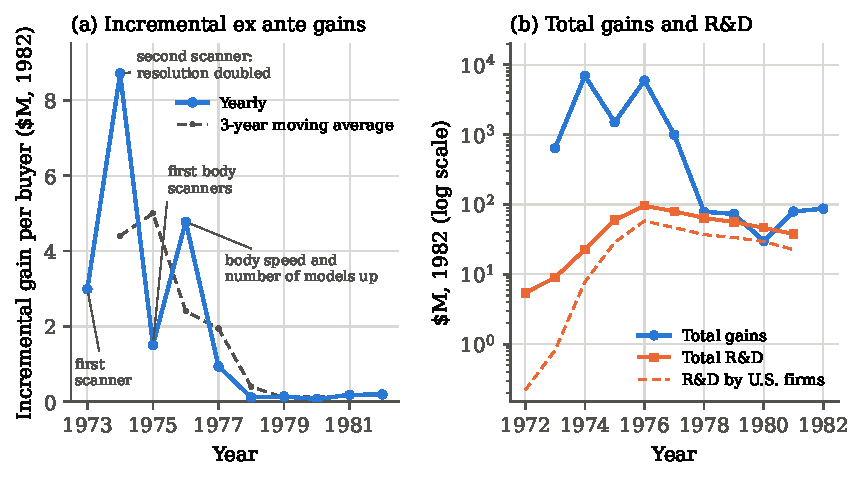
\includegraphics[width=\textwidth]{figures/ch10/trajtenberg_profile.pdf}
\caption{The time profile of the gains from innovation in CT scanners. Panel (a) shows the incremental ex ante gain per
buyer, with the 1973 value equal to the indirect estimate $\frac{K_0}{k}$, and its centered three-year moving average,
which is our computation. Panel (b) shows total gains $TW_t$ and research and development spending on a logarithmic
scale. The 1968--71 research total is a four-year aggregate and is omitted. Source: Trajtenberg (1985), Tables 9, 11
and 12.}
\label{fig:10-ct-profile}
\end{figure}

Second, the single largest gain came from the second scanner model, the EMI CT 1000 of 1974. Its design was almost
identical to the first EMI scanner, except that its resolution was almost doubled. The improvement transformed CT from a
demonstration of feasibility into a widely useful diagnostic tool (p.~78). Trajtenberg calls the early appearance of
such a big winner the ``Ford-T effect,'' after the Model T. Third, research spending tracked the level of activity in
the field with a one-year lead, but it was not closely related to the gains. The ratio of gains to research was about 80
to 1 for 1968--77, with research taken up to 1976. It was 1.4 for 1978--82, and in 1980 research spending exceeded the
benefits (p.~80).\footnote{The first ratio reproduces from Tables~11 and 12. Total gains of \$16,023.7 million in
1973--77 against total research of \$199.02 million in 1968--76 give 80.5. With the same one-year research lead and
no discounting, the two tables give $\frac{348.3}{284.40} = 1.22$ for 1978--82. The paper does not state the
definition behind its figure of 1.4 (our computation).}
Average returns are therefore a poor guide to policy. The question is less whether public support for research is
warranted than until when it should last. In CT, support was socially valuable in the early stages but not after 1976.
Trajtenberg notes that the British Department of Health supported the construction of the first prototype at EMI in
1970--72. An American neurologist, W.~H.~Oldendorf, had independently developed a similar device but could not pursue
it for lack of support (p.~80, n.~80). He presents the profile as evidence, from one case, that innovation can follow a
wave-like pattern.

\subsection{Robustness}\label{sec:10-ct-robustness}

Trajtenberg checks several of his choices, mostly in footnotes. The checks are scattered through the preceding
subsections, and we gather them here. The hedonic function was estimated in three forms, and Box-Cox comparisons
ranked the linear-log form first in half of the twelve cases (p.~37, n.~33). In the diffusion equation, a concave
ceiling gave very similar results to the linear one (pp.~67--68). The concave ceiling corresponds to exponentially
distributed reservation prices. Letting the incremental gains shift the speed of diffusion gave an effect that was
significant but very small (p.~68, n.~64). Repeat purchases are credited only with the incremental gain of their
year, so total gains are a lower bound in this respect (p.~70, n.~67). Adding profits of up to half of revenue to
the benefits would barely change the rate of return (p.~73). Returns to U.S. research and to total research serve
as upper and lower bounds on the true rate (pp.~71--72). Finally, the ex ante and ex post welfare measures are both
reported, and they differ by a factor of about seven (\cref{sec:10-ct-welfare}).

\subsection{Interpretation, critiques and contribution}\label{sec:10-ct-assessment}

Trajtenberg's study established that the magnitude of a product innovation can be measured by the consumer surplus it
creates, computed from an estimated discrete-choice model in characteristics space. Each step of the later literature
appears here in early form. Welfare comes from a log-sum surplus function. The nested logit is used to draw market
boundaries. Prices are related to characteristics through a hedonic function, and the per-buyer gains are linked to
diffusion and to research spending. \Citet{Petrin2002} builds on the template. \Citet[p.~238]{Bresnahan1997} writes
that Hausman takes on the question of the slope of $dd$ ``following Trajtenberg (1989).''

The limitations are of three kinds. The first concerns identification of price sensitivity. There are no instruments,
the residual-price coefficients have the wrong sign, and $\alpha$ is imported from another segment
(\cref{sec:10-ct-signal}). Because the money value of every gain divides by $\alpha$, the welfare numbers inherit this
uncertainty in full. The second concerns functional form. The MNL imposes IIA within branches, buyer heterogeneity is
absent after 1975, and the logit adds an entropy term for every new model (\cref{prop:10-clones,prop:10-entropy}). The
quadratic net utility extrapolates the value of large changes in characteristics. The estimated tastes change from year
to year, and the choice between ex ante and ex post measures changes the answer by a factor of seven. The second-stage
estimate of $\lambda$ carries little information about substitution between branches, as \eqref{eq:10-traj-lambda-implied} shows.
The third concerns interpretation. The buyers are hospitals, whose valuations may diverge from those of patients
(\cref{sec:10-ct-consumer}). The total gains rest on a reduced-form diffusion equation, and the value of the first scanner
is an indirect extrapolation from it.

These limitations do not overturn the qualitative conclusions. Early innovations in CT created large value relative
to their cost, gains concentrated in a few improvements, and returns to research fell sharply as the technology matured.
The precise numbers are less secure. The next case study, \citeauthor{Petrin2002}'s minivan, addresses several of the
weaknesses at once. It uses instruments for price, random coefficients disciplined by micro data, and a supply side
that lets rivals' prices respond. It also decomposes the welfare gain into the parts due to observed characteristics
and to the logit errors.

\section{Case study: the minivan (Petrin 2002)}\label{sec:10-petrin}

\citet{Petrin2002} measures the welfare created by the minivan, a vehicle that Chrysler introduced in 1984 and that
its rivals imitated within two years. The paper answers two questions. The first is substantive. How large were the
gains to consumers and to each producer, and how were they shared? The second is methodological. How can a
researcher who has only market-level data discipline the random coefficients that govern substitution, and therefore
welfare? Petrin's answer to the second question, the use of \emph{micro moments}, is now a standard part of demand
estimation (\cref{sec:08-micro-moments}). \Cref{tab:10-petrin-map} at the end of the section maps the study.
We follow the paper from its question to its contribution, as in
\cref{sec:10-hausman}.\footnote{Petrin writes $\gamma_k$ for the scale of the random coefficient on characteristic $k$,
$\gamma_{mi}$, $\gamma_{sw}$, $\gamma_{su}$ and $\gamma_{pv}$ for the family-vehicle interactions, and $\tau$ for the
cost parameters. In his text the income-group price coefficients are $\alpha_0$, $\alpha_1$ and $\alpha_2$, while his
Table 4 labels them $\alpha_1$, $\alpha_2$ and $\alpha_3$. We write $\sigma_k$, $\pi_{\mathrm{mv}}$, $\pi_{\mathrm{sw}}$,
$\pi_{\mathrm{su}}$, $\pi_{\mathrm{pv}}$ and $\gamma$, and we follow the table for the price coefficients. Page and
table numbers in this section refer to the journal article.}

\subsection{The question}\label{sec:10-petrin-question}

New products improve the standard of living, and firms introduce them to earn the temporary market power of a first
mover (p.~705). Petrin estimates three objects for the minivan. The first is the compensating variation of consumers,
including the gains of households that bought other vehicles whose prices fell when the minivan arrived. The second
is the change in producer surplus. It combines Chrysler's first-mover profits, the cannibalization of its own station
wagons, and the losses imposed on Ford and General Motors (GM). The third is the profit that the imitators dissipated
when they entered.

The question matters for the theory of \cref{sec:10-imperfect}. There we saw that a new good changes welfare through
the surplus of its own buyers and through the prices of existing goods. \Cref{tab:10-bresnahan-2x2} called the second
channel ``Competition,'' and \cref{sec:10-bresnahan} criticized \citet{Hausman1997} for holding rivals' prices fixed.
Petrin re-solves the pricing equilibrium of the whole automobile market with and without minivans. His estimates
therefore measure the Competition cell, together with Chrysler's repricing of its own wagons, in one equilibrium
calculation.

The method matters as much as the answer. Random coefficients are imprecisely estimated from market shares alone
(\cref{sec:08-instruments}). Welfare numbers inherit that imprecision, and they inherit the dependence on the
idiosyncratic logit shock described in \cref{sec:10-charspace}. Petrin's abstract states the main finding in these
terms. Models estimated without micro data yield much larger welfare numbers, ``primarily because the micro data
appear to free the model from a heavy dependence on the idiosyncratic logit `taste' error'' (p.~705).

\subsection{The minivan innovation}\label{sec:10-petrin-setting}

Ford proposed a vehicle called the ``Mini/Max'' in the early 1970s (p.~707). It was a boxlike vehicle that obtained
interior space from its height, with front-wheel drive that lowered the passenger floor. Ford's management gave the
idea little support because it feared cannibalizing the firm's strong station wagon sales. This is the private
incentive problem of \cref{sec:10-imperfect} in its purest form. A firm that owns close substitutes values a new
product only net of the profits it diverts from them.

The financially troubled Chrysler Corporation introduced the Dodge Caravan in 1984. It sold 170,000 units in its first
year. GM introduced the Astro and Safari in 1985, and Ford introduced the Aerostar in 1986. Both rivals were unprepared
for the Caravan's success. They built their minivans on truck platforms with rear-wheel drive, so these vehicles
handled more like downsized full-size vans than like passenger cars. Chrysler kept its lead by adding a larger engine
and a second sliding door. Fourteen years after the introduction, six firms sold 13 minivans, and Chrysler held 44
percent of a market of 1.16 million vehicles. Station wagon sales peaked at 950,000 in 1984 and fell to 300,000 over
the next seven years (p.~707).

Table~3 of the paper shows the substitution in shares of total vehicle sales. Minivans rose from 1.58 percent in 1984 to
9.93 percent in 1993. Station wagons held about 10 percent in 1981--83 (10.51, 10.27 and 10.32 percent), fell to 8.90
percent in 1984, and reached 3.02 percent in 1993. The combined share of minivans and wagons stayed between 9.65 and
12.95 percent over 1981--93. Petrin reads this negative comovement as evidence of a positive covariance in the tastes
for the two vehicle types (p.~718). The demand model is built to capture that covariance.

\subsection{Data}\label{sec:10-petrin-data}

The paper combines two data sets (pp.~712--713). The market data cover all 2,407 nameplates sold in the United States
from 1981 to 1993 with annual sales above 1,000 vehicles. They come from the \textit{Automotive News Market Data
Book} and \textit{Ward's Automotive Yearbook}. The characteristics are acceleration (horsepower per unit of curb
weight), size (length times width times height), drive type, fuel efficiency (miles per dollar), and a luxury proxy
(air conditioning standard). Quantity and list price refer to the base model. Nameplates in adjacent years whose
horsepower, wheelbase, width and length change by less than 10 percent are treated as the same model. This rule leaves
916 independent observations, and the standard errors allow arbitrary correlation of the errors of the same model over
time (p.~716, n.~11).

The consumer data come from the Consumer Expenditure Survey (CEX) for 1987--92. Almost 30,000 household records
approximate the joint distribution of demographics in the United States. The CEX automobile supplement links the
demographics of 2,660 new-vehicle buyers to the vehicles they bought. Among them are 120 minivan buyers, 63 station
wagon buyers, 131 sport-utility buyers and 23 full-size van buyers. These samples are too small for a consumer-level
choice model, since about 200 kinds of vehicles are sold each year but only about 400 purchases are recorded annually
(p.~713, n.~8). They are large enough to estimate a few averages precisely. Other annual inputs are the number of
households $M$, gasoline prices and the growth of gross national product. The random coefficients model without micro
data also uses a lognormal income distribution estimated from the March Current Population Survey (p.~713, n.~9).

\Cref{tab:10-petrin-cex} reproduces the demographic averages of Table~2 of the paper. They are the targets of the micro
moments. New-vehicle buyers had a mean income of \$36,113, about \$13,000 above the U.S. mean of \$23,728 (incomes
in 1982--84 dollars). Minivan buyers had the largest families of all buyer groups, 3.86 members against 2.58 in the
population. They also had the highest share of household heads aged 30 to 60, 78 percent against 55 percent. Table~1 of
the paper adds that minivans were larger than the average vehicle (size 0.87 against 0.71). Of them, 78 percent had air
conditioning as standard (27 percent of all vehicles), and their mean list price was \$10,060 against \$9,867 for all
vehicles. Chrysler accounted almost entirely for the 63 percent of minivan sales with front-wheel drive (p.~716).

\begin{table}[htbp]
\centering
\caption{Demographics of the U.S. population and of new-vehicle buyers, 1987--92}\label{tab:10-petrin-cex}
\small
\setlength{\tabcolsep}{5pt}
\begin{tabular}{@{}lccccccc@{}}
\toprule
 & \multicolumn{2}{c}{United States} & \multicolumn{5}{c}{Buyers of} \\
\cmidrule(lr){2-3}\cmidrule(l){4-8}
 & Mean & Std.\ dev. & New vehicles & Minivans & Wagons & Sport-utilities & Full-size vans \\
\midrule
Income (\$)  & 23,728 & 21,255 & 36,113 & 39,476 & 40,196 & 41,569 & 31,164 \\
Family size  & 2.58   & 1.53   & 2.87   & 3.86   & 3.17   & 2.97   & 3.47   \\
Midage       & 0.55   & 0.49   & 0.64   & 0.78   & 0.73   & 0.74   & 0.65   \\
\bottomrule
\end{tabular}

\smallskip
\begin{minipage}{0.95\textwidth}
\footnotesize Source: \citet[Table~2]{Petrin2002}, from the Consumer Expenditure Survey. Income is in 1982--84
CPI-adjusted dollars. Family size is the number of household members. Midage is an indicator for a household head
aged between 30 and 60 inclusive.
\end{minipage}
\end{table}

\subsection{The demand model}\label{sec:10-petrin-model}

Consumers are households $i$ with income $y_i$, family size $fs_i$, an indicator $\mathit{mid}_i$ for a head aged 30 to
60, and unobserved tastes. Each household buys one new vehicle $j \in \{1, \dots, J\}$ in a year or buys none ($j = 0$).
Petrin specifies the conditional indirect utility (p.~710)
\begin{equation}\label{eq:10-petrin-utility}
  u_{ij} = \alpha_i \ln(y_i - p_j) + x_j\beta + \sum_{k} \sigma_k \nu_{ik} x_{jk}
           + \ln(fs_i)\,\nu_{i,\mathrm{fv}} \sum_{g \in \mathcal{G}} \pi_g d_{jg} + \xi_j + \epsilon_{ij},
  \qquad j = 1, \dots, J .
\end{equation}
The first term is the utility of the composite good bought with the income left after the vehicle. The row vector
$x_j$ holds a constant, the five characteristics, four vehicle-type dummies, the percentage change in gross national
product and a quadratic time trend (Table~4, note). The set $\mathcal{G} = \{\mathrm{mv}, \mathrm{sw}, \mathrm{su},
\mathrm{pv}\}$ collects the four \emph{family vehicle} types: minivans, station wagons, sport-utility vehicles and
full-size passenger vans. The dummy $d_{jg}$ equals one when vehicle $j$ is of type $g$. The unobserved product quality
is $\xi_j$, and $\epsilon_{ij}$ is type-I extreme value.

Three features of \eqref{eq:10-petrin-utility} carry the economics.

\casehead{Income effects} The marginal utility of income varies across the three income terciles,
\begin{equation*}
  \alpha_i = \begin{cases}
    \alpha_1 & \text{if } y_i < \bar y_1, \\
    \alpha_2 & \text{if } \bar y_1 \le y_i < \bar y_2, \\
    \alpha_3 & \text{if } y_i \ge \bar y_2,
  \end{cases}
\end{equation*}
where $\bar y_1$ and $\bar y_2$ split the population into three equal groups. The utility cost of a higher price is
\begin{equation}\label{eq:10-petrin-dudp}
  \frac{\partial u_{ij}}{\partial p_j} = -\frac{\alpha_i}{y_i - p_j} ,
\end{equation}
so price sensitivity falls with income within a group, and the three $\alpha_g$ let the curvature differ across groups.
This is the Cobb-Douglas income specification of \citet{BerryLevinsohnPakes1995} studied in \cref{sec:08-income}, with
group-specific coefficients. Conditional on all tastes, the logit formulas give the individual share derivatives
\begin{equation*}
  \frac{\partial s_{ij}}{\partial p_j} = -\frac{\alpha_i}{y_i - p_j}\,s_{ij}(1 - s_{ij}), \qquad
  \frac{\partial s_{ij}}{\partial p_k} = \frac{\alpha_i}{y_i - p_k}\,s_{ij}s_{ik} \quad (k \ne j).
\end{equation*}
Market derivatives integrate these over households.

\casehead{Random tastes for characteristics} Household $i$ draws a taste $\nu_{ik}$ for each characteristic $k$,
scaled by $\sigma_k$. Petrin draws the $\nu_{ik}$ independently from a $\chi^2(3)$ distribution truncated at its 95th
percentile (p.~711). He gives two reasons. The distribution is bounded above and below, and it skews heterogeneity in
the direction of positive taste. Taken as written, the draws lie between 0 and 7.81, with mean about 2.63 and standard
deviation about 1.83 (our computation). The paper does not say whether the draws are \emph{centered}, that is, whether
their mean is subtracted before they enter utility. The random coefficient on the constant makes the value of buying any new vehicle,
relative to the outside option, heterogeneous across households.

\casehead{Demographic tastes for family vehicles} The taste of household $i$ for a family vehicle of type $g$ is
$\pi_g \ln(fs_i)\,\nu_{i,\mathrm{fv}}$. The draw $\nu_{i,\mathrm{fv}}$ is common to all four types, and family size
scales it. Conditional on family size, the covariance between the tastes for minivans and for station wagons is
\begin{equation}\label{eq:10-petrin-cov}
  \Cov\bigl(\pi_{\mathrm{mv}}\ln(fs_i)\nu_{i,\mathrm{fv}},\; \pi_{\mathrm{sw}}\ln(fs_i)\nu_{i,\mathrm{fv}} \bigm| fs_i\bigr)
  = \pi_{\mathrm{mv}}\pi_{\mathrm{sw}}\,\bigl(\ln fs_i\bigr)^2\,\Var(\nu_{i,\mathrm{fv}}) .
\end{equation}
It rises with $\pi_{\mathrm{mv}}$ and $\pi_{\mathrm{sw}}$ and with family size. Substitution between minivans and
wagons can therefore arise for two reasons (p.~710). Large families prefer both types, or the two types share other
observed characteristics such as size.

The outside option is to buy no new vehicle. We write its utility as $u_{i0} = \alpha_i\ln y_i + \epsilon_{i0}$, the
normalization of \cref{sec:08-income}. Conditional on the household's demographics $D_i = (y_i, fs_i, \mathit{mid}_i)$
and tastes $\nu_i$, the probability of buying $j$ is the logit formula (p.~711)
\begin{equation}\label{eq:10-petrin-sij}
  s_{ij} = \frac{\exp V_{ij}}{\exp\bigl(\alpha_i \ln y_i\bigr) + \sum_{l=1}^{J} \exp V_{il}} ,\qquad
  V_{ij} = \alpha_i\ln(y_i - p_j) + \delta_j + \mu_{ij},
\end{equation}
with base utility $\delta_j = x_j\beta + \xi_j$ and household-specific term
\begin{equation*}
  \mu_{ij} = \sum_k\sigma_k\nu_{ik}x_{jk} + \ln(fs_i)\,\nu_{i,\mathrm{fv}}\sum_g \pi_g d_{jg} .
\end{equation*}
Price is not part of $\delta_j$. It enters only through the income
term, so the $\alpha_g$ are nonlinear parameters, as in \cref{sec:08-income}. The market share is $s_j = \int s_{ij}\,
\dd P(D_i, \nu_i)$, where $D_i$ follows the empirical distribution of the CEX and $\nu_i$ the truncated $\chi^2(3)$
distribution. Petrin calls the elements of $\beta$ \emph{base coefficients} (Table~4). If the draws are centered,
$\mu_{ij}$ has mean zero and $\delta_j$ is the mean utility of product $j$, net of the income term. Otherwise
$\delta_j$ is that utility for a household whose draws are all zero, and the mean taste for characteristic $k$ is
$\beta_k + 2.63\,\sigma_k$.

The demand side has 24 parameters: three price coefficients, eleven base coefficients, six random-coefficient scales
and four family-vehicle interactions. Eleven of them describe family vehicles and income effects: the three
$\alpha_g$, the four type dummies and the four $\pi_g$. The micro moments speak most directly to these eleven.

\subsection{Supply and the counterfactual equilibrium}\label{sec:10-petrin-supply}

The supply side follows \citet{BerryLevinsohnPakes1995} (pp.~711--712). Multiproduct firms $f = 1, \dots, F$ set prices
in a static Bertrand-Nash equilibrium. Marginal cost is log-linear in observed cost characteristics $W_j$ and an
unobserved component $\omega_j$,
\begin{equation}\label{eq:10-petrin-mc}
  \ln mc_j = W_j\gamma + \omega_j .
\end{equation}
Firm $f$ earns $\Pi_f = M\sum_{j\in\mathcal{J}_f}(p_j - mc_j)\,s_j(p, x; \theta)$, and the first-order conditions are
\begin{equation}\label{eq:10-petrin-foc}
  s_j(p, x; \theta) + \sum_{r \in \mathcal{J}_f}(p_r - mc_r)\frac{\partial s_r(p, x; \theta)}{\partial p_j} = 0,
  \qquad j \in \mathcal{J}_f .
\end{equation}
In matrix form these are \eqref{eq:08-foc-matrix}, and inverting them gives the markup formula \eqref{eq:08-markup},
$p - mc = -[(\Omega\odot\Delta)^\top]^{-1}s$. Given demand estimates and observed prices, this formula recovers each
$mc_j$ \citep[eq.~3]{Petrin2002}.

A rearrangement of \eqref{eq:10-petrin-foc} is useful for reading the counterfactual. Separate the own-product term
and divide by $-\frac{\partial s_j}{\partial p_j} > 0$:
\begin{align}
  0 &= s_j + (p_j - mc_j)\frac{\partial s_j}{\partial p_j}
       + \sum_{r\in\mathcal{J}_f,\, r\ne j}(p_r - mc_r)\frac{\partial s_r}{\partial p_j}, \notag\\
  p_j - mc_j &= \frac{s_j}{-\frac{\partial s_j}{\partial p_j}}
       + \sum_{r\in\mathcal{J}_f,\, r\ne j}(p_r - mc_r)\,D_{jr},
  \qquad D_{jr} = \frac{\frac{\partial s_r}{\partial p_j}}{-\frac{\partial s_j}{\partial p_j}} . \label{eq:10-petrin-diversion}
\end{align}
Here $D_{jr}$ is the diversion ratio from $j$ to $r$ (\cref{ch:diffprod}). The markup on $j$ is a single-product
markup plus the margins the firm earns on the sales that a higher $p_j$ diverts to its other products. When Chrysler
adds a minivan $m$ that is a substitute for its station wagons, a new positive term $(p_m - mc_m)D_{jm}$ appears in the
markup of each Chrysler wagon $j$. Other things equal, Chrysler raises the prices of its wagons. Rival firms gain no
term for the minivan. Their markups change through the first term, which falls when entry makes their demand more
elastic, and through changes in diversion among their own products.

The counterfactual removes all minivans from the choice set and solves \eqref{eq:10-petrin-foc} for the remaining
products, holding marginal costs, characteristics and $\xi_j$ fixed (p.~712). Call the solution $p^{cf}$ and the
observed prices $p^0$. The change in the variable profit of firm $f$ due to the minivan is $\Pi_f(p^0, mc) -
\Pi_f(p^{cf}, mc)$, and summing over firms gives the change in producer surplus. A second counterfactual removes only
the Ford and GM minivans, which measures how much of Chrysler's profit the imitators dissipated. The profit function
ignores the 25 percent tariff on Japanese minivans, which made up a small part of minivan sales (p.~712, n.~6).

\subsection{Compensating variation with income effects}\label{sec:10-petrin-cv}

Petrin measures consumer welfare by a compensating variation whose benchmark is the standard of living attained with
minivans (p.~720). The counterfactual environment has no minivans, and the other vehicles sell at $p^{cf}$. For a
household with all tastes $(D_i, \nu_i, \epsilon_i)$ held fixed, let $\mathcal{J}^1$ be the choice set with minivans
and $\mathcal{J}^0$ the set without them. The household's compensation $CV_i$ solves
\begin{equation}\label{eq:10-petrin-cvdef}
  \max_{j \in \mathcal{J}^0 \cup \{0\}} u_{ij}\bigl(y_i + CV_i,\, p^{cf}\bigr)
  = \max_{j \in \mathcal{J}^1 \cup \{0\}} u_{ij}\bigl(y_i,\, p^{0}\bigr) \equiv U_i^1 .
\end{equation}
This is the compensating variation of removing the minivans, which equals the equivalent variation of introducing
them. It is the measure \eqref{eq:10-cv-income} of \cref{sec:10-cs-welfare}, and the discrete-choice analog of
\cref{prop:10-cv-newgood}, whose reference utility is also the one attained with the new good.

With the utility \eqref{eq:10-petrin-utility} the compensation has a closed form. Write $v_{ij} = \delta_j + \mu_{ij}
+ \epsilon_{ij}$ for the part of utility that does not involve money, with $p_0 = 0$ and $v_{i0} = \epsilon_{i0}$.
For each alternative $j \in \mathcal{J}^0\cup\{0\}$, define the compensation that would make $j$ alone reach $U_i^1$:
\begin{align*}
  \alpha_i\ln\bigl(y_i + c_{ij} - p^{cf}_j\bigr) + v_{ij} &= U_i^1, \\
  y_i + c_{ij} - p^{cf}_j &= \exp\Bigl(\frac{U_i^1 - v_{ij}}{\alpha_i}\Bigr), \\
  c_{ij} &= p^{cf}_j - y_i + \exp\Bigl(\frac{U_i^1 - v_{ij}}{\alpha_i}\Bigr).
\end{align*}
The left side of \eqref{eq:10-petrin-cvdef} increases in $CV_i$, and it first reaches $U_i^1$ when the cheapest of
these compensations is paid. Hence
\begin{equation}\label{eq:10-petrin-cvi}
  CV_i = \min_{j \in \mathcal{J}^0 \cup \{0\}} \Bigl\{ p^{cf}_j - y_i + \exp\Bigl(\frac{U_i^1 - v_{ij}}{\alpha_i}\Bigr) \Bigr\}.
\end{equation}
The formula has a useful implication for households that did not buy a minivan. If household $i$ chose $j \in
\mathcal{J}^0$ at $p^0$, then $U_i^1 = \alpha_i\ln(y_i - p^0_j) + v_{ij}$, and the term for $j$ in
\eqref{eq:10-petrin-cvi} equals
\begin{equation*}
  p^{cf}_j - y_i + \exp\Bigl(\frac{\alpha_i\ln(y_i - p^0_j)}{\alpha_i}\Bigr) = p^{cf}_j - y_i + (y_i - p^0_j)
  = p^{cf}_j - p^0_j .
\end{equation*}
A non-buyer's compensation is therefore at most the price change of the vehicle she chose. It equals that change if
and only if her vehicle remains a best choice at prices $p^{cf}$ and the compensated income $y_i + p^{cf}_j - p^0_j$.
At that income vehicle $j$ yields exactly $U_i^1$, so the condition says that no alternative reaches $U_i^1$ with
less compensation. Remaining best at the original income $y_i$ does not suffice, because income enters utility
through $\ln(y_i - p_k)$. Extra income then raises the utility of expensive vehicles more than that of cheap ones.
For these households, as Petrin notes (p.~720), compensation is
determined entirely by the price changes that the minivan caused. Averaging $CV_i$ over simulated households and
multiplying by $M$ gives the aggregate measure.

Petrin also splits the compensation of minivan buyers into two parts (Table~8). Suppose utility were quasi-linear,
$u_{ij} = \delta_j - \alpha p_j + \mu_{ij} + \epsilon_{ij}$. Let $j$ be the buyer's minivan and $k$ her best
alternative in $\mathcal{J}^0$ at $p^{cf}$. Then
\begin{equation}\label{eq:10-petrin-decomp}
  CV_i = \underbrace{\frac{(\delta_j - \alpha p^0_j + \mu_{ij}) - (\delta_k - \alpha p^{cf}_k + \mu_{ik})}{\alpha}}_{
  \text{observed characteristics}}
  + \underbrace{\frac{\epsilon_{ij} - \epsilon_{ik}}{\alpha}}_{\text{logit error}} .
\end{equation}
The first part is the value of the minivan's observed characteristics and price relative to the second choice. The
second part is the value of the idiosyncratic logit draws. With income effects the split is approximate (p.~722,
n.~13).

The logit benchmark explains why the second part can dominate. The next result, which we derive, extends
\cref{prop:10-logit-newgood} from the aggregate gain to the gain of the buyers of the new good.

\begin{proposition}[Who gains in a logit model]\label{prop:10-logit-buyer-cv}
Let $u_{ij} = V_j + \epsilon_{ij}$ with $V_j = \delta_j - \alpha p_j$ and $\epsilon_{ij}$ independent type-I extreme
value. Remove a set $\mathcal{N}$ of products whose total share is $s_{\mathcal{N}}$, holding all other prices fixed.
Then
\begin{enumerate}[label=(\alph*)]
  \item A consumer whose chosen product is not in $\mathcal{N}$ has $CV_i = 0$.
  \item The mean compensation of consumers who chose a product in $\mathcal{N}$ is
        $\frac{1}{\alpha}\,\frac{-\ln(1 - s_{\mathcal{N}})}{s_{\mathcal{N}}} \ge \frac{1}{\alpha}$.
\end{enumerate}
\end{proposition}

\begin{proof}
(a) The consumer's chosen product remains available at the same price, and her utilities are unchanged. Her maximum
utility is the same in both choice sets, so $CV_i = 0$.

(b) By \cref{lem:10-cv-quasilinear}, $CV_i = \frac{1}{\alpha}\bigl(\max_{j}u_{ij} - \max_{j\notin\mathcal{N}}u_{ij}\bigr)$.
By \cref{lem:10-logsum}, the expected maximum of $V_j + \epsilon_{ij}$ over a set $S$ is $\ln\sum_{j\in S}e^{V_j} +
\gamma_E$. Therefore, as in the proof of \cref{prop:10-logit-newgood},
\begin{align*}
  \E[CV_i] &= \frac{1}{\alpha}\Bigl(\ln\sum_{j}e^{V_j} - \ln\sum_{j\notin\mathcal{N}}e^{V_j}\Bigr)
            = -\frac{1}{\alpha}\ln\frac{\sum_{j\notin\mathcal{N}}e^{V_j}}{\sum_{j}e^{V_j}}
            = -\frac{1}{\alpha}\ln(1 - s_{\mathcal{N}}) .
\end{align*}
By part (a), $\E[CV_i] = s_{\mathcal{N}}\,\E[CV_i \mid \text{chose in } \mathcal{N}]$. Dividing by $s_{\mathcal{N}}$ gives
the formula. The inequality follows from $-\ln(1-s) \ge s$ for $s \in [0,1)$, as in \eqref{eq:10-logit-perbuyer}.
\end{proof}

Part (b) says that in a logit model the buyers of a product with a small share gain on average about $\frac{1}{\alpha}$
dollars, whatever the product is. Part (b) of \cref{prop:10-entropy} says why. For every product $n$,
\begin{equation*}
  \E[\epsilon_{in} \mid i \text{ chooses } n] = \gamma_E - \ln s_n ,
\end{equation*}
so a product with a small share is bought by consumers with large draws of $\epsilon_{in}$, and the model credits the
purchase to those draws. Its mean utility $V_n$ is low, so the observed component in \eqref{eq:10-petrin-decomp} tends
to be negative while the logit component is large. The markup has the same scale. \Cref{rem:10-logit-multiproduct}
showed that a multiproduct logit firm charges a common markup on all its products, $m_f = \frac{1}{\alpha(1 - S_f)}$,
where $S_f = \sum_{r\in\mathcal{J}_f}s_r$ is the firm's total share. Since each firm's share of all households is small,
every logit markup is close to $\frac{1}{\alpha}$. We return to both implications when we read Petrin's Tables 8 and 9.

\subsection{Estimation: market moments plus micro moments}\label{sec:10-petrin-estimation}

The estimator is the generalized method of moments (GMM) estimator of \citet{BerryLevinsohnPakes1995}, augmented by
moments from the CEX (pp.~713--716). The idea comes from \citet{ImbensLancaster1994}, who show that aggregate
information on the averages of micro variables can sharpen the estimates of a micro model.

\casehead{Micro moments} Petrin uses three sets of moments (p.~714). Let $P_{ig}(\theta) = \int\sum_{j\in g}s_{ij}(\theta)
\,\dd P(\nu_i)$ be the probability that a household with demographics $D_i$ buys a vehicle of type $g$, and let
$P_{i}(\theta) = \int \sum_{j\ge1}s_{ij}(\theta)\,\dd P(\nu_i)$ be its probability of buying any new vehicle. The first
set matches the purchase probability in each income group $h \in \{1,2,3\}$:
\begin{equation}\label{eq:10-petrin-mm1}
  \E\bigl[\indic\{i \text{ buys a new vehicle}\} \bigm| y_i \in h\bigr]
  = \frac{\int \indic\{y_i\in h\}\,P_i(\theta)\,\dd P(D_i)}{\int\indic\{y_i\in h\}\,\dd P(D_i)} .
\end{equation}
The second set matches the mean family size of the buyers of each family vehicle type $g \in \mathcal{G}$:
\begin{equation}\label{eq:10-petrin-mm2}
  \E\bigl[fs_i \bigm| i \text{ buys type } g\bigr] = \frac{\int fs_i\,P_{ig}(\theta)\,\dd P(D_i)}{\int P_{ig}(\theta)\,\dd P(D_i)} .
\end{equation}
The third set matches $\E[\mathit{mid}_i \mid i \text{ buys type } g]$, the probability that the household head is aged
30 to 60, in the same way. The left sides are CEX sample averages and the right sides are model predictions. There
are $3 + 4 + 4 = 11$ micro moments. \Cref{eq:10-petrin-mm2} is Bayes' rule applied to the purchase
probability, as in \eqref{eq:08-bayes}.

A simple identity shows what the family-size moments identify.

\begin{lemma}[What a conditional-mean moment measures]\label{lem:10-micro-moment}
For any demographic $D$ and purchase probability $P_{ig}$ with $\E[P_{ig}] > 0$,
\begin{equation*}
  \E\bigl[D_i \bigm| i \text{ buys type } g\bigr] = \E[D_i] + \frac{\Cov(D_i, P_{ig})}{\E[P_{ig}]} .
\end{equation*}
\end{lemma}

\begin{proof}
By \eqref{eq:10-petrin-mm2} the conditional mean is $\frac{\E[D_iP_{ig}]}{\E[P_{ig}]}$. Write $\E[D_iP_{ig}] =
\E[D_i]\E[P_{ig}] + \Cov(D_i, P_{ig})$ and divide by $\E[P_{ig}]$.
\end{proof}

The CEX gives $\E[fs_i] = 2.58$ and $\E[fs_i \mid \text{minivan}] = 3.86$, so the model must produce
$\frac{\Cov(fs_i, P_{i,\mathrm{mv}})}{\E[P_{i,\mathrm{mv}}]} = 1.28$.
In \eqref{eq:10-petrin-utility} family size enters the minivan's utility only through $\pi_{\mathrm{mv}}\ln(fs_i)
\nu_{i,\mathrm{fv}}$, apart from its correlation with income. The moment therefore pins down $\pi_{\mathrm{mv}}$, and the
other three moments pin down the other $\pi_g$. Likewise, the purchase probabilities by income group pin down how
the $\alpha_g$ shift purchases across the income distribution. Market shares alone identify these parameters only
through variation in choice sets and in demographics over time, which is weak in thirteen years of national data.

\casehead{Market moments} The first set of market moments matches predicted and observed shares, $s_j(\delta, \theta) =
s_j$ for every $j$. As in \cref{sec:08-inversion}, this is equivalent to solving for the vector $\delta(\theta)$ that
equates them \citep{Berry1994}. The second set states that the demand and cost unobservables are mean independent of
the observed characteristics of all vehicles in the year (p.~715):
\begin{equation}\label{eq:10-petrin-blpmom}
  \E\bigl[\xi_j(\theta_0) \bigm| X, W\bigr] = \E\bigl[\omega_j(\theta_0) \bigm| X, W\bigr] = 0 .
\end{equation}
The instruments approximate the optimal ones in the manner of \citet{BerryLevinsohnPakes1995}. A product's own
characteristics instrument for themselves. Cost variables excluded from demand instrument for price. So do the sums
of each characteristic over the firm's other products, $\sum_{j\ne l,\, j\in\mathcal{J}_f}x_{jk}$, and over rivals'
products, $\sum_{j\notin\mathcal{J}_f}x_{jk}$. These sums measure how crowded a product's neighborhood is, which shifts
its markup through \eqref{eq:10-petrin-diversion} \citep{BresnahanSternTrajtenberg1997}.

\casehead{The objective and its variance} Stack the market moments $G_1(\theta)$ and the micro moments $G_2(\theta)$ in
$G(\theta) = (G_1(\theta)^\top, G_2(\theta)^\top)^\top$, with $\E[G(\theta_0)] = 0$. Let $\hat G(\theta)$ be the sample
analog and $a(\tilde\theta)$ a consistent estimate of the ``square root'' of the inverse of the moments' asymptotic
variance, computed at a preliminary estimate $\tilde\theta$. Following \citet{Hansen1982}, the two-step estimator is
(p.~715)
\begin{equation}\label{eq:10-petrin-gmm}
  \hat\theta = \argmin_{\theta\in\Theta}\; \tilde G(\theta)^\top\tilde G(\theta), \qquad
  \tilde G(\theta) = a(\tilde\theta)\,\hat G(\theta) .
\end{equation}
The two sets of moments come from independent samples, the vehicle market and the CEX. Let $n$ be the size of the
market sample, and suppose the CEX sample size $n_2$ satisfies $\frac{n_2}{n} \to \lambda \in (0,\infty)$. Write
$V_G$ for the asymptotic variance of $\sqrt{n}\,\hat G(\theta_0)$. Independence makes $V_G$ block diagonal. Since
$\sqrt{n}\,\hat G_2 = \sqrt{\frac{n}{n_2}}\,\sqrt{n_2}\,\hat G_2$, the micro block is $\frac{1}{\lambda}$ times the
asymptotic variance of $\sqrt{n_2}\,\hat G_2(\theta_0)$. Let $a$ and $\Gamma$ be the probability limits of $a(\tilde\theta)$ and
$\frac{\partial\tilde G(\theta_0)}{\partial\theta}$. The scaled moments $\sqrt{n}\,\tilde G(\theta_0)$ then have
asymptotic variance $V = aV_Ga^\top$, and the asymptotic variance of $\sqrt{n}(\hat\theta - \theta_0)$ is
\begin{equation}\label{eq:10-petrin-avar}
  (\Gamma^\top\Gamma)^{-1}\,\Gamma^\top V\Gamma\,(\Gamma^\top\Gamma)^{-1} .
\end{equation}
This is the usual sandwich for a GMM estimator with identity weight on the normalized moments
(\cref{app:econometrics}). Petrin writes $V = \E[\tilde G(\theta_0)\tilde G(\theta_0)^\top]$ (p.~715). Read literally,
that is the variance of a sample average, which is of order $\frac{1}{n}$, so the sandwich needs the factor $n$ of
our definition. If $a = V_G^{-\frac{1}{2}}$, then $V = I$ and \eqref{eq:10-petrin-avar} reduces to the efficient
GMM variance $(\Gamma^\top\Gamma)^{-1}$. The micro block of $V_G$ reflects CEX sampling error, which is large when a
buyer group is small or the CEX sample is small relative to the market sample.

\casehead{Computation} One evaluation of the objective proceeds as follows.
\begin{enumerate}[label=(\roman*)]
  \item Draw households from the CEX records and taste vectors $\nu_i$ from the truncated $\chi^2(3)$ distribution.
        Hold the draws fixed across evaluations.
  \item For trial nonlinear parameters $(\alpha_g, \sigma_k, \pi_g)$, invert the shares to obtain $\delta(\theta)$ by
        the contraction of \cref{sec:08-inversion}.
  \item Recover $\xi_j = \delta_j - x_j\beta$, compute markups from \eqref{eq:08-markup}, and recover $\omega_j = \ln(p_j -
        b_j) - W_j\gamma$, where $b_j$ is the markup. The linear parameters $(\beta,\gamma)$ can be concentrated out.
  \item Compute the model's micro predictions, such as \eqref{eq:10-petrin-mm1} and \eqref{eq:10-petrin-mm2}, from
        the same draws.
  \item Form \eqref{eq:10-petrin-gmm} and search over the nonlinear parameters.
\end{enumerate}
Because the micro moments only add terms to the objective, the method adds little computational burden to the BLP
estimator (p.~706).

\casehead{Identification} Petrin's footnote~5 (p.~709) explains how market data identify heterogeneity. Suppose
three cars differ only in interior space, two of them spacious, and each has a third of the market. In a second
market one spacious car is missing. If the remaining spacious car takes two-thirds of the market, its buyers
substitute on space, which reveals a strong and heterogeneous taste for space. If the two remaining cars split the
market, there is no evidence of heterogeneity. Identification of this kind requires large changes in choice sets. The
micro moments supply a second source, the covariance between demographics and choices in
\cref{lem:10-micro-moment}.

\citet{BerryLevinsohnPakes2004} develop a third source, consumers' reported second choices, which measure substitution
directly. They note that consumer attribute data, together with a changing choice set, are useful for explaining
substitution and welfare for minivans. They find other automotive choices less closely tied to commonly observed
attributes \citep[p.~70, n.~1]{BerryLevinsohnPakes2004}. They also stress that second-choice data from one cross
section cannot identify the level of price elasticities. \citet{BerryHaile2024} give the formal nonparametric
identification argument for micro data (\cref{sec:08-bh24}).

\subsection{Results}\label{sec:10-petrin-results}

\casehead{Demand parameters} \Cref{tab:10-petrin-demand,tab:10-petrin-rc} reproduce Tables~4 and 5 of the paper.
Moving from the OLS logit to the instrumental variables (IV) logit almost doubles the price coefficient, from 0.07 to
0.13. Berry, Levinsohn and Pakes found the same pattern, and it shows that instrumenting matters (p.~719). Many random
coefficients differ significantly from zero, so Wald tests reject both logit models in favor of the random
coefficient models.

The random coefficients model estimated from market data alone (column~3 of \cref{tab:10-petrin-demand} and
column~1 of \cref{tab:10-petrin-rc}) is imprecise. The paper reports that only six of the 24 demand parameters have
$z$-statistics above one, and that none of the eight family-vehicle coefficients does. Adding the micro moments
changes the picture. Twenty-one of the 24 parameters then have $z$-statistics above one. The paper reports that all
eleven coefficients related to family vehicles and income effects have $z$-statistics above three (p.~719).\footnote{Counting from the printed estimates and standard errors, we find seven ratios above one in the model
without micro data. The extra one is the front-wheel-drive coefficient, $-5.24$ (3.09), which Table~4 prints without
a star. In the model with micro data, ten of the eleven family-vehicle and income ratios exceed three. The full-size
van interaction, 0.42 (0.21), has a ratio of about two.}
The parameters closest to the added information gain the most precision. The standard error of $\pi_{\mathrm{mv}}$,
for example, falls from 2.62 to 0.10.

The estimates with micro data have an intuitive structure. The base coefficients on the four family-vehicle dummies
are negative, while the four $\pi_g$ are positive and precise. Relative to a car with the same observed
characteristics, household $i$ values a vehicle of type $g$ at $\beta_g + \pi_g\ln(fs_i)\,\nu_{i,\mathrm{fv}}$. A
one-person household has $\ln fs_i = 0$, so it values type $g$ at $\beta_g < 0$ whether or not the draws are centered.
For a household with a positive draw, the taste rises with family size. The draw is independent of demographics
(p.~710), so the average taste is $\beta_g + \pi_g\E[\ln fs_i]\,\E[\nu_{i,\mathrm{fv}}]$. With centered draws it equals
$\beta_g$. With uncentered draws $\E[\nu_{i,\mathrm{fv}}] \approx 2.63$, and Jensen's inequality gives $\E[\ln fs_i]
\le \ln\E[fs_i] = \ln 2.58$, where 2.58 is the CEX mean family size for 1987--92 (Table~2, p.~717). The largest resulting bound,
for station wagons, is $-1.31 + 0.28 \times 2.63 \times \ln 2.58 \approx -0.61$, and it stays negative for any mean
family size below 5.9. Under either normalization the
average household therefore values each family-vehicle type below a comparable car (our computation).

The scale of the random coefficient on miles per dollar is precisely estimated, at 2.58 (0.14). Since the draws of
\cref{sec:10-petrin-model} have a standard deviation of about 1.83, the implied standard deviation of the taste for
miles per dollar is about 4.7 (our computation). Tastes for fuel economy are therefore heterogeneous.

\begin{table}[htbp]
\centering
\caption{Petrin's demand estimates: price and base coefficients}\label{tab:10-petrin-demand}
\small
\setlength{\tabcolsep}{3.4pt}
\begin{tabular}{@{}lcccc@{}}
\toprule
 & OLS logit & IV logit & Random coefficients & Random coefficients \\
 &  &  &  & and micro data \\
 & (1) & (2) & (3) & (4) \\
\midrule
\multicolumn{5}{@{}l}{\textit{A. Price coefficients}} \\
$\alpha_1$ (low income)    & 0.07 (0.01)$^{**}$ & 0.13 (0.01)$^{**}$ & 4.92 (9.78)           & 7.52 (1.24)$^{**}$ \\
$\alpha_2$ (middle income) &                    &                    & 11.89 (21.41)         & 31.13 (4.07)$^{**}$ \\
$\alpha_3$ (high income)   &                    &                    & 37.92 (18.64)$^{**}$  & 34.49 (2.56)$^{**}$ \\
\midrule
\multicolumn{5}{@{}l}{\textit{B. Base coefficients}} \\
Constant                  & $-10.03$ (0.32)$^{**}$ & $-10.04$ (0.34)$^{**}$ & $-12.74$ (5.65)$^{**}$ & $-15.67$ (4.39)$^{**}$ \\
Horsepower per weight     & 1.48 (0.34)$^{**}$     & 3.78 (0.44)$^{**}$     & 3.40 (39.79)           & $-2.83$ (8.16) \\
Size                      & 3.17 (0.26)$^{**}$     & 3.25 (0.27)$^{**}$     & 4.60 (24.64)           & 4.80 (3.57)$^{*}$ \\
Air conditioning standard & $-0.20$ (0.06)$^{**}$  & 0.21 (0.08)$^{**}$     & $-1.97$ (2.23)         & 3.88 (2.21)$^{*}$ \\
Miles per dollar          & 0.18 (0.06)$^{**}$     & 0.05 (0.07)            & $-0.54$ (3.40)         & $-15.79$ (0.87)$^{**}$ \\
Front-wheel drive         & 0.32 (0.05)$^{**}$     & 0.15 (0.06)$^{**}$     & $-5.24$ (3.09)         & $-12.32$ (2.36)$^{**}$ \\
Minivan                   & 0.09 (0.14)            & $-0.10$ (0.15)         & $-4.34$ (13.16)        & $-5.65$ (0.68)$^{**}$ \\
Station wagon             & $-1.12$ (0.06)$^{**}$  & $-1.12$ (0.07)$^{**}$  & $-20.52$ (36.17)       & $-1.31$ (0.36)$^{**}$ \\
Sport-utility             & $-0.41$ (0.09)$^{**}$  & $-0.61$ (0.10)$^{**}$  & $-3.10$ (10.76)        & $-4.38$ (0.41)$^{**}$ \\
Full-size van             & $-1.73$ (0.16)$^{**}$  & $-1.89$ (0.17)$^{**}$  & $-28.54$ (235.51)      & $-5.26$ (1.30)$^{**}$ \\
Percent change in GNP     & 0.03 (0.01)$^{**}$     & 0.03 (0.01)$^{**}$     & 0.08 (0.02)$^{**}$     & 0.24 (0.02)$^{**}$ \\
\bottomrule
\end{tabular}

\smallskip
\begin{minipage}{0.97\textwidth}
\footnotesize Source: \citet[Table~4]{Petrin2002}. Standard errors in parentheses. $^{*}$ $z$-statistic above one.
$^{**}$ $z$-statistic above two (stars as printed). A quadratic time trend is included in all specifications. The
logit models (columns 1--2) have one price coefficient and no income effects. In columns 3--4 the $\alpha_g$ multiply
$\ln(y_i - p_j)$. In columns 1--2 the base coefficients are mean tastes. In columns 3--4 the coefficient on the change in GNP,
which has no random term, is also a mean taste. The other base coefficients are mean tastes only if the taste draws
are centered, which the paper does not state (\cref{sec:10-petrin-model}). Estimation uses 2,407
nameplate-years (916 independent models), 1981--93.
\end{minipage}
\end{table}

\begin{table}[htbp]
\centering
\caption{Petrin's random coefficient estimates}\label{tab:10-petrin-rc}
\small
\begin{tabular}{@{}lcc@{}}
\toprule
 & No micro data & CEX micro data \\
 & (1) & (2) \\
\midrule
\multicolumn{3}{@{}l}{\textit{Scales $\sigma_k$ of the random coefficients}} \\
Constant                  & 1.46 (0.87)$^{*}$     & 3.23 (0.72)$^{**}$ \\
Horsepower per weight     & 0.10 (14.15)          & 4.43 (1.60)$^{**}$ \\
Size                      & 0.14 (8.60)           & 0.46 (1.07) \\
Air conditioning standard & 0.95 (0.55)$^{*}$     & 0.01 (0.78) \\
Miles per dollar          & 0.04 (1.22)           & 2.58 (0.14)$^{**}$ \\
Front-wheel drive         & 1.61 (0.78)$^{**}$    & 4.42 (0.79)$^{**}$ \\
\midrule
\multicolumn{3}{@{}l}{\textit{Family-size interactions $\pi_g$}} \\
Minivan, $\pi_{\mathrm{mv}}$          & 0.97 (2.62)   & 0.57 (0.10)$^{**}$ \\
Station wagon, $\pi_{\mathrm{sw}}$    & 3.43 (5.39)   & 0.28 (0.09)$^{**}$ \\
Sport-utility, $\pi_{\mathrm{su}}$    & 0.59 (2.84)   & 0.31 (0.09)$^{**}$ \\
Full-size van, $\pi_{\mathrm{pv}}$    & 4.24 (32.23)  & 0.42 (0.21)$^{**}$ \\
\bottomrule
\end{tabular}

\smallskip
\begin{minipage}{0.75\textwidth}
\footnotesize Source: \citet[Table~5]{Petrin2002}, where the parameters are called $\gamma_k$, $\gamma_{mi}$,
$\gamma_{sw}$, $\gamma_{su}$ and $\gamma_{pv}$. Standard errors in parentheses. Stars as in \cref{tab:10-petrin-demand}.
The logit models of \cref{tab:10-petrin-demand} set all these parameters to zero.
\end{minipage}
\end{table}

\casehead{Costs} \Cref{tab:10-petrin-cost} reproduces Table~6 of the paper. It regresses the log of estimated
marginal cost on cost characteristics, which gives the parameters $\gamma$ of \eqref{eq:10-petrin-mc}. Petrin
reports that the car characteristics enter with the expected sign and significant coefficients (p.~720). The
front-wheel-drive coefficient, 0.01 (0.01), is an exception. The elasticities of marginal cost
are 0.84 (0.03) with respect to horsepower per weight, 1.28 (0.04) with respect to weight and 0.23 (0.04) with
respect to miles per gallon. Standard air conditioning raises log cost by 0.24 (0.01). Japanese and European
production carry cost premia of 0.12 (0.01) and 0.47 (0.03) in logs. The coefficient on $\ln q$ is $-0.05$ (0.01),
which indicates mild economies of scale.

\begin{table}[htbp]
\centering
\caption{Petrin's cost-side estimates}\label{tab:10-petrin-cost}
\small
\begin{tabular}{@{}lc@{\qquad}lc@{}}
\toprule
Variable & Estimate & Variable & Estimate \\
\midrule
Constant                         & 1.50 (0.08) & Trend                  & $-0.01$ (0.01) \\
$\ln$(horsepower per weight)     & 0.84 (0.03) & Japan                  & 0.12 (0.01) \\
$\ln$(weight)                    & 1.28 (0.04) & Japan $\times$ trend   & $-0.01$ (0.01) \\
$\ln$(miles per gallon)          & 0.23 (0.04) & Europe                 & 0.47 (0.03) \\
Air conditioning standard        & 0.24 (0.01) & Europe $\times$ trend  & $-0.01$ (0.01) \\
Front-wheel drive                & 0.01 (0.01) & $\ln q$                & $-0.05$ (0.01) \\
\bottomrule
\end{tabular}

\smallskip
\begin{minipage}{0.86\textwidth}
\footnotesize Source: \citet[Table~6]{Petrin2002}, where the parameters are called $\tau$. The dependent variable is
the log of estimated marginal cost. Standard errors in parentheses. Estimation uses the 2,407 nameplate-years of
\cref{tab:10-petrin-demand}.
\end{minipage}
\end{table}

\casehead{Prices on entry} Panel~A of \cref{tab:10-petrin-prices} shows the vehicles whose prices fell most when the
minivan entered in 1984. The Caravan's closest substitutes were top-selling large sedans and station wagons. Wagons
had the largest percentage decreases, and large family sedans the largest dollar decreases (\$100 to \$150). Panel~B
shows that some prices rose. Two of the four largest increases are Chrysler's own wagons, the LeBaron (\$297) and the
Dodge Aries K (\$170). This is the diversion term of \eqref{eq:10-petrin-diversion}: once Chrysler sells minivans, a
lost wagon sale is partly recaptured as a minivan sale. The other two increases are rival wagons. Random coefficients
can produce such increases because entry removes the buyers most willing to switch, leaving a less elastic residual
demand. The paper's note states that Bertrand-Nash pricing with random coefficients does not determine the signs of
the price changes a priori. Compare \cref{prop:10-logit-rivals}, where symmetric logit demand forces all rivals'
prices down.

\begin{table}[htbp]
\centering
\caption{Equilibrium prices with and without the minivan, 1984 (selected vehicles)}\label{tab:10-petrin-prices}
\small
\setlength{\tabcolsep}{5pt}
\begin{tabular}{@{}lrrrr@{}}
\toprule
 & \multicolumn{2}{c}{Price (\$)} & & \\
\cmidrule(lr){2-3}
Vehicle (segment) & With minivan & Without minivan & $\Delta$ price (\$) & $\Delta$ price (\%) \\
\midrule
\multicolumn{5}{@{}l}{\textit{A. Largest decreases on entry}} \\
GM Oldsmobile Toronado (large sedan)  & 15,502 & 15,643 & $-141$ & $-0.90$ \\
GM Buick Riviera (large sedan)        & 15,379 & 15,519 & $-139$ & $-0.89$ \\
GM Buick Electra (large sedan)        & 12,843 & 12,978 & $-135$ & $-1.04$ \\
GM Chevrolet Celebrity (wagon)        & 8,304  & 8,431  & $-127$ & $-1.51$ \\
GM Pontiac 6000 (wagon)               & 9,273  & 9,397  & $-123$ & $-1.31$ \\
GM Oldsmobile Ciera (wagon)           & 9,591  & 9,714  & $-123$ & $-1.27$ \\
GM Buick Century (wagon)              & 8,935  & 9,056  & $-121$ & $-1.34$ \\
GM Oldsmobile Firenza (wagon)         & 7,595  & 7,699  & $-104$ & $-1.35$ \\
\midrule
\multicolumn{5}{@{}l}{\textit{B. Largest increases on entry}} \\
Chrysler LeBaron (wagon)              & 9,869  & 9,572  & 297 & 3.10 \\
Volkswagen Quattro (wagon)            & 13,263 & 13,079 & 184 & 1.41 \\
Chrysler (Dodge) Aries K (wagon)      & 7,829  & 7,659  & 170 & 2.22 \\
AMC Eagle (wagon)                     & 10,178 & 10,069 & 109 & 1.08 \\
\bottomrule
\end{tabular}

\smallskip
\begin{minipage}{0.92\textwidth}
\footnotesize Source: \citet[Table~7]{Petrin2002}, model with micro data, 1982--84 CPI-adjusted dollars. The signs
in the percentage column of Panel~A are ours. The original prints magnitudes only. Panel~A of the original also
lists two Cadillac large sedans ($-126$ and $-125$ dollars), omitted here.
\end{minipage}
\end{table}

\casehead{Consumer welfare in 1984} Gains from lower prices are large. In 1984 the households that did not buy a
minivan received \$157 million of the \$367 million of consumer gains, almost 43 percent (pp.~720 and 727).
\Cref{tab:10-petrin-cv} reproduces Table~8, which summarizes the compensation of minivan buyers under the four demand
models.

\begin{table}[htbp]
\centering
\caption{Compensating variation of 1984 minivan buyers under four demand models}\label{tab:10-petrin-cv}
\small
\begin{tabular}{@{}lrrrr@{}}
\toprule
 & OLS logit & IV logit & Random & Random coefficients \\
 &  &  & coefficients & and micro data \\
\midrule
\multicolumn{5}{@{}l}{\textit{Compensating variation (\$)}} \\
\quad Median & 9,573  & 5,130  & 1,217 & 783 \\
\quad Mean   & 13,652 & 7,414  & 3,171 & 1,247 \\
\multicolumn{5}{@{}l}{\textit{Welfare change from difference in (\$)}} \\
\quad Observed characteristics ($\delta_j + \mu_{ij}$) & $-81{,}469$ & $-44{,}249$ & $-820$ & 851 \\
\quad Logit error ($\epsilon_{ij}$)                     & 95,121    & 51,663    & 3,991  & 396 \\
\multicolumn{5}{@{}l}{\textit{Income of minivan buyers (\$)}} \\
\quad Estimate from model          & 23,728    & 23,728    & 99,018 & 36,091 \\
\quad Difference from actual (CEX) & $-15{,}748$ & $-15{,}748$ & 59,542 & $-3{,}385$ \\
\bottomrule
\end{tabular}

\smallskip
\begin{minipage}{0.92\textwidth}
\footnotesize Source: \citet[Table~8]{Petrin2002}, 1982--84 CPI-adjusted dollars. Compensating variation is
evaluated at equilibrium prices without minivans. The decomposition is the average difference in the value of observed
and unobserved characteristics between first and second choices, as in \eqref{eq:10-petrin-decomp}. In the logit
models the purchase decision is independent of income, so the mean income of buyers is the mean U.S. household income.
The two decomposition rows sum to the mean in every column, and the last row equals the model estimate minus the CEX
mean of \$39,476.
\end{minipage}
\end{table}

The logit models imply mean compensations of \$13,652 (OLS) and \$7,414 (IV). Adding the price of the vehicle, the
implied mean willingness to pay is \$22,374 and \$16,136 (p.~720). Petrin finds these values inconsistent with
Chrysler's profit maximization and implausible given the many cheaper vehicles available. The decomposition shows the
source. Minivan buyers would need \$95,121 (OLS) or \$51,663 (IV) for the loss of their idiosyncratic minivan taste,
while they ``strongly dislike'' the minivan's observed characteristics relative to their second choice.

\Cref{prop:10-logit-buyer-cv} predicts this pattern. By part (b), minivan buyers should gain on average about
$\frac{1}{\alpha}$, since minivans were a small fraction of all households' choices in 1984. The paper does not state
the units of price in the logit models. We infer that they are thousands of 1982--84 dollars, from two pieces of
evidence. First, Petrin notes that the ratio of the two mean logit markups, \$13,904 to \$7,551, almost equals the
ratio of the price coefficients (p.~723, n.~14). Second, the logit markup $\frac{1}{\alpha(1 - S_f)}$ is close to
$\frac{1}{\alpha}$ when firms' shares are small. With $\alpha = 0.07$ per thousand dollars, $\frac{1}{\alpha}$ is about
\$14,300, and Table~9 places the OLS logit markups between \$13,647 and \$14,297 (10th and 90th percentiles). The IV
logit gives $\frac{1}{0.13}$, about \$7,700, against markups between \$7,413 and \$7,765. Figure~1 reports compensating
variation in thousands of the same dollars (p.~724), which fits this reading.
The reported means lie slightly below these values, which the proposition gives as lower bounds at fixed prices.
Rounding of $\alpha$ in Table~4 explains almost all of the gap, since coefficients printed as 0.07 and 0.13 may be as
large as 0.0749 and 0.1349.
By \cref{prop:10-entropy}(b), the minivan's small share means that its
buyers have large logit draws, so the observed component is negative.

The random coefficients model without micro data lowers the mean compensation to \$3,171 and the logit component to
\$3,991. The observed component is still negative ($-\$820$). This model also implies that only the wealthiest, least
price-sensitive households buy new vehicles. The mean income of its minivan buyers is \$99,018, almost \$60,000 above
the CEX value. With micro moments, the mean compensation falls to \$1,247. The observed component becomes positive
(\$851) and the logit component falls to \$396. The implied mean income of minivan buyers, \$36,091, is about \$3,000
below the CEX value of \$39,476 (pp.~722--723).

\begin{figure}[htbp]
\centering
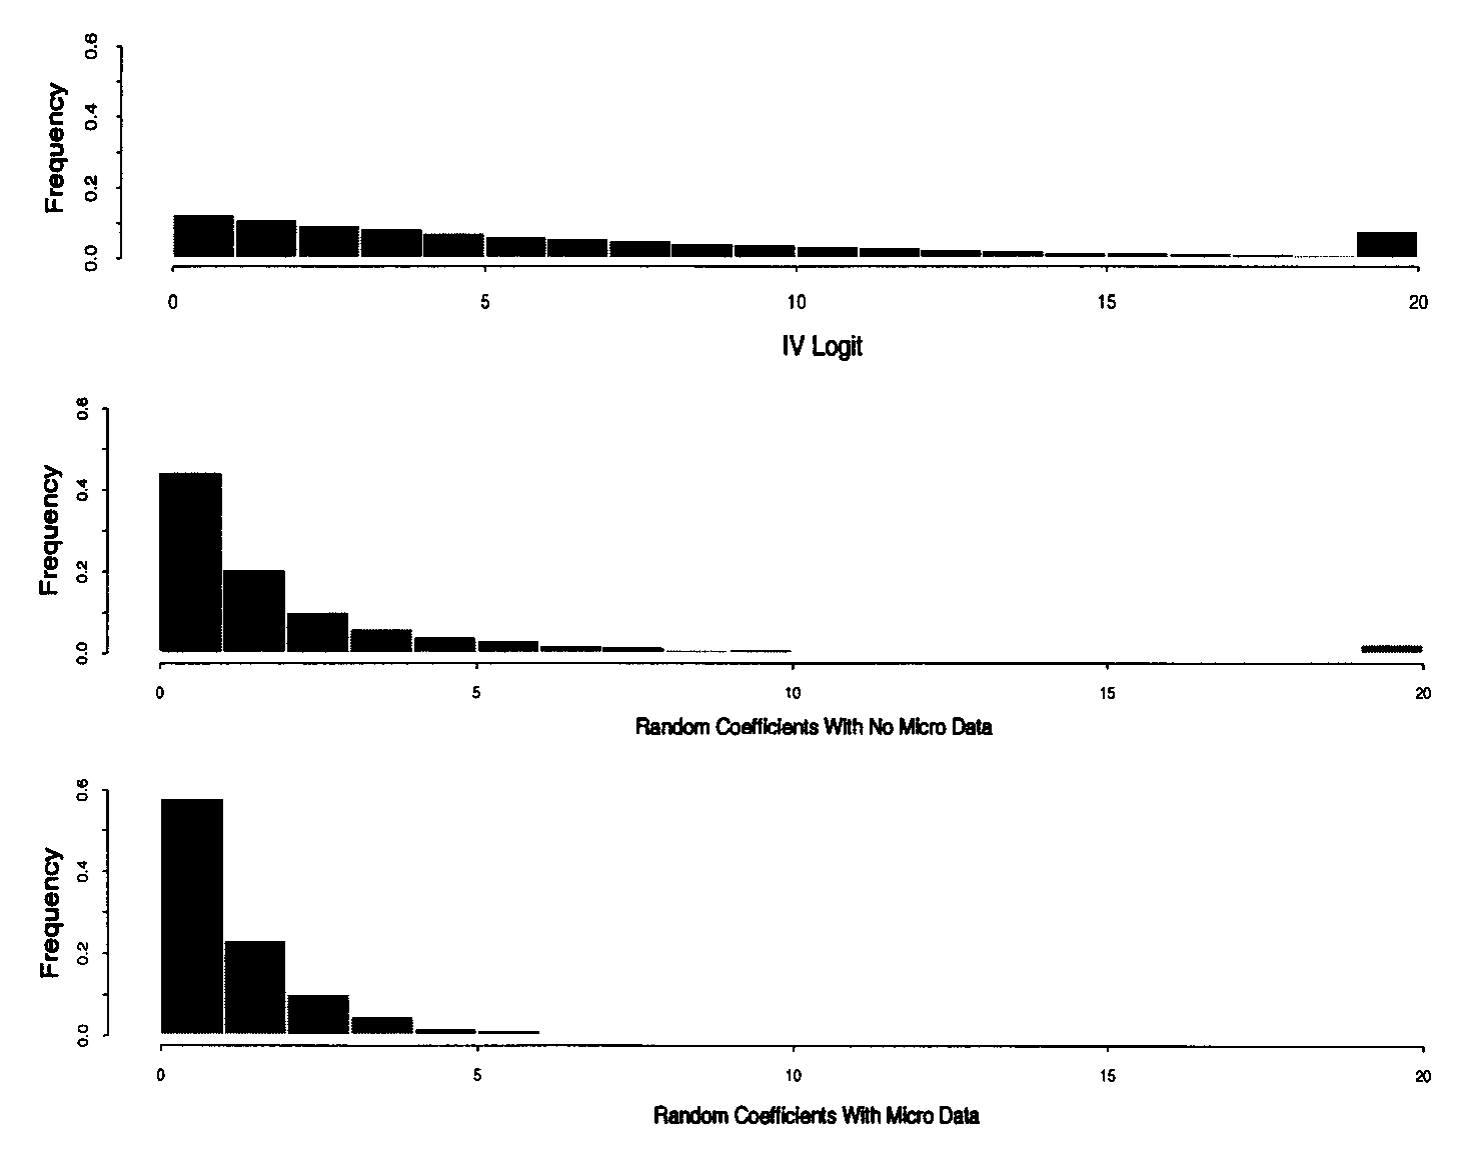
\includegraphics[width=\textwidth]{figures/ch10/petrin_fig1.png}
\caption{Distribution of compensating variation for 1984 minivan buyers, in thousands of 1982--84 dollars. The top
panel is the IV logit model, the middle panel the random coefficients model without micro data, and the bottom panel
the random coefficients model with micro data. The bar at 20 appears to collect the upper tail. Source: Petrin (2002), Figure~1.}
\label{fig:10-petrin-cv-hist}
\end{figure}

\Cref{fig:10-petrin-cv-hist} shows the whole distribution of compensation. Under the IV logit, 10 percent of
minivan buyers would need at least \$20,000 (p.~723). With random coefficients, the tail is much thinner, but many
buyers would still need thousands of dollars. Adding the micro moments removes most of the ``extreme-tastes'' tail.
Petrin prefers the full model on the cumulative weight of this evidence.

\casehead{Markups} \Cref{tab:10-petrin-markups} reproduces Table~9. The two logit models imply mean markups of \$13,904
and \$7,551. Their ratio is almost exactly the ratio of the price coefficients, as the logit markup formula
$\frac{1}{\alpha(1 - S_f)}$ implies (p.~723, n.~14). The same formula explains the tiny dispersion. The standard
deviation is 1.85 percent of the mean in both logit columns, because firms' shares are small and identical across the
two columns.
A Yugo and a Cadillac then carry nearly the same dollar markup. Marginal cost, which is price minus this markup, is
negative for 73.7 percent (OLS) and 22.6 percent (IV) of vehicles. Petrin notes that many logit own-price elasticities
are below one, which is inconsistent with static profit maximization (p.~723, n.~15). The example shows how a bias in
demand passes into the supply side. The random coefficient models imply only positive marginal costs. Their mean
percentage markups are 40.7 percent without micro data and 16.7 percent with them. Both lie within the range of earlier
estimates, 15 to 40 percent in \citet{BerryLevinsohnPakes1995} and an average of 38 percent in \citet{Goldberg1995}
(p.~725, n.~16).

\begin{table}[htbp]
\centering
\caption{Implied markups under Bertrand-Nash pricing, 1981--93 (2,407 models)}\label{tab:10-petrin-markups}
\small
\begin{tabular}{@{}lrrrrrr@{}}
\toprule
 & OLS logit & IV logit & \multicolumn{2}{c}{Random coefficients} & \multicolumn{2}{c}{RC and micro data} \\
\cmidrule(lr){4-5}\cmidrule(l){6-7}
Statistic & (\$) & (\$) & (\$) & (\%) & (\$) & (\%) \\
\midrule
Median              & 13,834 & 7,513 & 2,593 & 36.7 & 1,439 & 15.0 \\
Mean                & 13,904 & 7,551 & 4,017 & 40.7 & 1,753 & 16.7 \\
10th percentile     & 13,647 & 7,413 & 1,628 & 27.8 & 819   & 11.2 \\
90th percentile     & 14,297 & 7,765 & 8,357 & 62.6 & 2,856 & 24.8 \\
Standard deviation  & 257    & 140   & 4,089 & 14.0 & 1,229 & 6.2 \\
Negative marginal costs (\%) & 73.7 & 22.6 & \multicolumn{2}{c}{0} & \multicolumn{2}{c}{0} \\
\bottomrule
\end{tabular}

\smallskip
\begin{minipage}{0.92\textwidth}
\footnotesize Source: \citet[Table~9]{Petrin2002}, 1982--84 CPI-adjusted dollars. Percentage markups are markups
divided by observed prices. They are not reported for the logit models because estimated marginal costs are negative
for many vehicles.
\end{minipage}
\end{table}

Table~10 of the paper follows sales-weighted percentage markups by segment for 1983--87, using the model with micro
data. Minivans earned the highest markups in every year they were sold (19.19 percent in 1984, 19.43 in 1985, 17.33
in 1986 and 16.31 in 1987). Station wagons earned less than minivans in every year. In four of the five years their
markups also fell below those of the column for all other vehicles. The pairs are 18.27 against 18.85 percent in 1983,
16.81 against 17.12 in 1985, 15.82 against 16.43 in 1986 and 13.86 against 14.79 in 1987. In 1984 wagons were slightly
above that column, at 17.83 against 17.72 percent. Petrin's text says that wagon markups ``consistently fell below the
market average'' (p.~725), which his table does not bear out for 1984.
Petrin attributes the minivan premium partly to its location in a less crowded region of product space. Overall,
markups fell as the number of vehicle choices grew from 157 in 1983 to 198 in 1987 (p.~725).

\casehead{Producer surplus and dissipation} \Cref{tab:10-petrin-profits} combines Tables~11 and 12. Chrysler's variable
profits rose by \$202.5 million, or 14.38 percent, in 1984 relative to a world without minivans. The gain grew to
\$504.1 million (32.50 percent) by 1988. Petrin states that by the end of 1987 Chrysler's minivans had generated almost
\$1.5 billion in profits, against a reported development cost of \$700 million (p.~726).\footnote{The Chrysler column
of Table~11 sums to \$1,008.8 million over 1984--87 and to \$1,512.9 million over 1984--88. The paper does not show how
its \$1.5 billion figure is computed. The development cost was reported in \textit{Time} on March 21, 1983. A
\$400 million retooling cost reported in \textit{Fortune} is a lower bound on development costs (p.~726, n.~17).}
Ford and GM were both hurt. The paper summarizes their losses as 1 to 2 percent of variable profits a year, which for
high-volume GM amounted to more than \$100 million in every year of Table~11. Ford's profit rose in 1986, the year its
Aerostar arrived. The industry as a whole lost
in 1984 and 1985, so ex post the industry would have been willing to pay Chrysler not to introduce the minivan
(p.~727). Once Ford and GM sold minivans, they dissipated \$126 million of Chrysler's profits over 1985--88, the
profit on about 76,000 minivans. Chrysler's minivan was differentiated enough to keep much of its market power.

\begin{table}[htbp]
\centering
\caption{Changes in variable profits due to the minivan, and Chrysler's losses to imitators}\label{tab:10-petrin-profits}
\small
\begin{tabular}{@{}lrrrrrrrrr@{}}
\toprule
 & Industry & \multicolumn{2}{c}{Chrysler} & \multicolumn{2}{c}{Ford} & \multicolumn{2}{c}{GM} &
 \multicolumn{2}{c}{Chrysler, dissipation} \\
\cmidrule(lr){3-4}\cmidrule(lr){5-6}\cmidrule(lr){7-8}\cmidrule(l){9-10}
Year & (\%) & (\$m) & (\%) & (\$m) & (\%) & (\$m) & (\%) & (\$m) & (\%) \\
\midrule
1984 & $-0.21$ & 202.5 & 14.38 & $-31.8$ & $-1.16$ & $-155.8$ & $-1.50$ &          &         \\
1985 & $-0.13$ & 259.1 & 13.99 & $-37.4$ & $-1.29$ & $-171.0$ & $-1.63$ & $-6.06$  & $-0.16$ \\
1986 & 0.14    & 201.1 & 12.42 & 54.7    & 1.84    & $-119.9$ & $-1.09$ & $-22.72$ & $-1.99$ \\
1987 & 0.17    & 346.1 & 23.27 & $-22.8$ & $-0.66$ & $-174.5$ & $-2.14$ & $-42.35$ & $-2.25$ \\
1988 & 0.65    & 504.1 & 32.50 & $-24.7$ & $-0.70$ & $-235.4$ & $-2.90$ & $-55.68$ & $-2.63$ \\
\bottomrule
\end{tabular}

\smallskip
\begin{minipage}{0.95\textwidth}
\footnotesize Source: \citet[Tables~11 and 12]{Petrin2002}, model with micro data, millions of 1982--84 dollars. The
first eight columns compare profits with minivans to profits with all minivans removed. The last two compare
Chrysler's profits with all minivans to its profits with the Ford and GM minivans removed.
\end{minipage}
\end{table}

\casehead{Total welfare} \Cref{tab:10-petrin-welfare} reproduces Table~13. Over 1984--88 the compensating variation
sums to \$2,804.55 million and producer profits rise by \$105.54 million, for a welfare gain of \$2,910.09 million.
Producer profits fell in 1984 and 1985 and rose afterward. In every row the welfare change equals the compensating
variation plus the change in producer profits. The gains to society far exceed both the cost of developing the vehicle
and the innovator's private return (p.~727).

\begin{table}[htbp]
\centering
\caption{Change in U.S. welfare from the minivan, 1984--88 (millions of 1982--84 dollars)}\label{tab:10-petrin-welfare}
\small
\begin{tabular}{@{}lrrr@{}}
\toprule
Year & Compensating variation & Change in producer profits & Welfare change \\
\midrule
1984  & 367.29   & $-36.68$ & 330.61 \\
1985  & 625.04   & $-25.07$ & 599.97 \\
1986  & 439.93   & 27.30    & 467.23 \\
1987  & 596.59   & 29.75    & 626.34 \\
1988  & 775.70   & 110.24   & 885.94 \\
\midrule
Total & 2,804.55 & 105.54   & 2,910.09 \\
\bottomrule
\end{tabular}

\smallskip
\begin{minipage}{0.8\textwidth}
\footnotesize Source: \citet[Table~13]{Petrin2002}, model with micro data. Producer profits are the variable profits of
all firms, from the equilibrium with and without minivans.
\end{minipage}
\end{table}

The 1984 numbers can be cross-checked against Table~8. Minivans took 1.58 percent of 10.66 million vehicle sales in
1984, or about 168,000 vehicles (Table~3). Minivan buyers received \$367.29 million less the \$157 million that went to
other households. That leaves about \$1,250 per minivan buyer, close to the mean of \$1,247 in Table~8.

\subsection{Robustness*}\label{sec:10-petrin-robustness}

The paper's main robustness check is the comparison across its four demand models, and we gather its results here.
Instrumenting almost doubles the logit price coefficient (p.~719). Wald tests reject both logit models in favor of
the random coefficients models (p.~719). Without micro data only 6 of the 24 demand parameters have $z$-statistics
above one, and with them 21 of the 24 do (p.~719). Across the four models the mean compensation of 1984 minivan
buyers falls from \$13,652 to \$7,414, \$3,171 and \$1,247 (\cref{tab:10-petrin-cv}). Two further checks discriminate
among the models. The logit models imply negative marginal costs for many vehicles (\cref{tab:10-petrin-markups}).
The random coefficients model without micro data predicts a mean income of minivan buyers far above the CEX value,
while the full model comes close (\cref{tab:10-petrin-cv}). The paper reports no estimates under other taste
distributions. The tail of compensation in \cref{fig:10-petrin-cv-hist} therefore rests on the truncated
$\chi^2(3)$ assumption, which \cref{sec:10-petrin-critique} discusses.

\subsection{Interpretation, limitations and critiques}\label{sec:10-petrin-critique}

The paper's central lesson concerns the logit error. Its share in the welfare of minivan buyers is a diagnostic of how
much the answer rests on the functional form. That share falls from about 700 percent of the mean (the observed part
being negative) under the OLS logit to 32 percent with micro data (\$396 of \$1,247). Even the preferred model credits a
third of the buyers' gain to the $\epsilon_{ij}$ draws. A pure characteristics model would remove that component
entirely \citep{BerryPakes2007}, and \cref{sec:10-charspace} showed that such models value close substitutes much less.
\citet{AckerbergRysman2005} propose a related correction that lets the variance of the logit error shrink as the
product space fills.

Several assumptions shape the level of the estimates. The income term $\alpha_i\ln(y_i - p_j)$ fixes how compensation
scales with income, and the truncated $\chi^2(3)$ distribution fixes the tails of taste heterogeneity. Since compensation
is a nonlinear function of tastes, \cref{fig:10-petrin-cv-hist} depends on these tails. The market size is the number of
U.S. households, so the outside option absorbs all households that buy no new vehicle. The counterfactual holds the
characteristics and the $\xi_j$ of the other vehicles fixed. Ford and GM might have repositioned their wagons or
introduced their own minivans earlier in a world in which Chrysler did not. The model is static, so welfare covers
only 1984--88 and is not discounted. Prices are list prices of base models, without rebates or options.

The counterfactual also defines the object being valued. It removes all minivans, including the Ford and GM models,
so the \$2.9 billion values the minivan as a class of vehicle. The value of any single firm's minivan is a narrower
question. The dissipation counterfactual of Table~12 answers it for the imitators.

Finally, the minivan dummy carries much of the new good's value. A minivan is a new combination of height, size and
front-wheel drive. Its mean taste and the dispersion of that taste ($\pi_{\mathrm{mv}}$) are identified from minivan
sales and from the CEX buyer averages. They are not predicted from tastes for existing characteristics. The
analysis is therefore an ex post valuation, which differs from the ex ante prediction that characteristics models
promise in \cref{sec:10-charspace}.

\subsection{Contribution}\label{sec:10-petrin-contribution}

The paper made two contributions. The first is the micro-moment technique. It brings aggregate information
about buyers into the BLP estimator at almost no computational cost, and it showed that such moments sharpen exactly
the parameters that matter for welfare. Micro moments are now routine in demand estimation (\cref{sec:08-micro}). The
second is the welfare accounting of a new good under oligopoly. Petrin measured how much of the consumer gain came
through competition (43 percent in 1984), how much the innovator earned, and how much the imitators dissipated. He
concludes that large improvements in consumers' standard of living arise from competition among firms that seek
temporary market power through new goods (p.~728).

\begin{table}[htbp]
\centering
\caption{Identification and counterfactual map of Petrin (2002)}
\label{tab:10-petrin-map}
\footnotesize
\renewcommand{\arraystretch}{1.1}
\begin{tabularx}{\textwidth}{@{}>{\raggedright\arraybackslash}p{2.6cm}>{\raggedright\arraybackslash}X@{}}
\toprule
Observed data & Prices, sales and characteristics of 2,407 U.S. nameplate-years, 1981--1993. CEX
  averages of the demographics of new-vehicle buyers, 1987--1992, and the CPS income distribution. \\
\addlinespace
Latent objects & Product quality $\xi_j$, cost shocks $\omega_j$, household tastes and incomes, and
  marginal costs. \\
\addlinespace
Estimated parameters & Price coefficients for three income groups, random-coefficient scales $\sigma_k$,
  family-vehicle interactions $\pi$, mean tastes and the cost coefficients $\gamma$. \\
\addlinespace
Identifying variation & Characteristics-based instruments for prices, as in BLP, plus micro moments that
  match purchase probabilities by income group and the family size and age of the buyers of each vehicle
  type. \\
\addlinespace
Maintained assumptions & Static multiproduct Bertrand-Nash pricing, log-linear marginal cost, the income
  term $\alpha_i\ln(y_i-p_j)$, exogenous characteristics, and a market size equal to the number of
  households. \\
\addlinespace
Counterfactual and what it holds fixed & Removal of all minivans, with the prices of the other vehicles
  re-solved. Marginal costs, characteristics and $\xi_j$ are held fixed. A second counterfactual removes
  only the Ford and GM minivans. \\
\addlinespace
Conclusion & The compensating variation is \$2,804.55 million over 1984--1988, and about 43 percent of the
  consumer gain in 1984 came through lower prices of other vehicles. Micro moments shrink the share of the
  logit errors in buyers' gains. \\
\addlinespace
One limitation & Rivals cannot reposition their products in the counterfactual, although they might have
  done so in a world without Chrysler's minivan. \\
\addlinespace
Source and our additions & The tables are Petrin's. \Cref{prop:10-logit-buyer-cv,lem:10-micro-moment} and the
  diversion form \eqref{eq:10-petrin-diversion} are ours. \\
\addlinespace
Tools in the appendices & \Cref{sec:A-gmm,sec:A-simulation,sec:B-fixedpoint}. \\
\bottomrule
\end{tabularx}
\end{table}

\section{Case study: complementarity and online news (Gentzkow 2007)}\label{sec:10-gentzkow}

Every discrete choice model of this chapter so far assumes that a consumer chooses one product. In those models the
new good can only draw consumers away from existing goods. The continuous demand systems of the chapter, such as the
AIDS system of \cref{sec:10-hausman}, are different, since they let spending spread over many brands.
\citet{Gentzkow2007} builds a discrete choice model in which consumers may choose
several goods at once, and in which the data decide whether goods are substitutes or complements. He applies it to the
\textit{Washington Post}, its online edition (the post.com) and the competing daily \textit{Washington Times}. We follow
the paper from its question to its contribution, and \cref{tab:10-gentzkow-map} at the end of the section maps
it.\footnote{Gentzkow writes $\sigma$ for the correlation of the
unobservables in his two-good model and $\Gamma$ for the interaction term. He writes $\gamma$ for the probability of a
news-day shock, $\lambda$ for the number of readers per copy, $\kappa$ for the transaction cost of online payment and
$\Psi$ for the fixed cost. We write $\rho$, $\Gamma_{AB}$ (or $\Gamma_r$ for bundle $r$), $\varpi$, $\kappa$, $\chi$ and
$F^{\mathrm{fix}}$. Page and table numbers in this section refer to the journal article.}

\subsection{The question}\label{sec:10-gentzkow-question}

Do new goods crowd out existing goods or complement them? Gentzkow opens with examples in which the answer surprised
the industry (p.~713). Record companies in the 1920s believed that radio broadcasts crowded out record sales, until
radio airplay turned out to raise them. A widely cited forecast predicted that computers would create a ``paperless
office,'' yet information technology sharply increased paper consumption. Newspaper executives in the early 2000s
debated whether free online editions siphon readers from print (p.~714, n.~4).

The answer matters for three reasons (pp.~713--714). It drives firms' decisions on entry, positioning and pricing.
It determines the welfare value of the new good and hence the bias of price indexes. It informs policy, such as rules
on cross-media mergers. Standard discrete choice models cannot answer the question. They assume that each consumer
chooses exactly one product, so all goods are perfect substitutes at the individual level (p.~714). The single-unit
assumption is reasonable for cars, and it is the main limitation of characteristics models for goods consumed together.
Gentzkow's model removes it.

A second difficulty is empirical. Frequent online readers are also frequent print readers. The pattern could mean that
the goods are complements. It could also mean that some consumers simply have a stronger taste for news. Separating
true complementarity from correlated tastes is the central identification problem of the paper (p.~714).

\subsection{A two-good model of bundles}\label{sec:10-gentzkow-model}

Consider two goods, $A$ and $B$. Each consumer buys at most one unit of each, so she chooses one of four
\emph{bundles}: nothing ($0$), $A$ only, $B$ only, or both ($AB$). Income not spent on the goods buys a composite good
whose utility is $\alpha$ per dollar. Let $u_r$ be the utility of bundle $r$ relative to the empty bundle. Gentzkow
specifies (p.~717, eq.~1)
\begin{equation}\label{eq:10-gentzkow-twogood}
  u_0 = 0, \qquad u_A = \delta_A - \alpha p_A + \nu_A, \qquad u_B = \delta_B - \alpha p_B + \nu_B, \qquad
  u_{AB} = u_A + u_B + \Gamma_{AB} .
\end{equation}
Here $\delta_A$ and $\delta_B$ are mean utilities, and $(\nu_A, \nu_B)$ are unobserved tastes. The parameters
$\delta_A$, $\delta_B$ and $\Gamma_{AB}$ are common to all consumers. The term $-\alpha p_j$ is the utility of the
composite good forgone, $\alpha(y - p_j) - \alpha y$. The \emph{interaction term}
\begin{equation*}
  \Gamma_{AB} = (u_{AB} - u_B) - (u_A - u_0)
\end{equation*}
is the discrete analog of a cross-partial derivative of utility. It measures how much the added utility of $A$ rises
when $B$ is consumed as well. Gentzkow assumes that $(\nu_A, \nu_B)$ is bivariate normal with unit variances and
correlation $\rho$. One unit variance is a normalization of scale. The other only simplifies exposition.

Demand per consumer is $Q_A = P_A + P_{AB}$ for good $A$ and $Q_B = P_B + P_{AB}$ for good $B$, where $P_r$ is the
probability of choosing bundle $r$. Because utility is quasi-linear, income effects are absent, and compensated and
uncompensated cross-price derivatives coincide. The standard definition of complements \citep{Samuelson1974} then reads
as follows (p.~717, Definition~1).

\begin{definition}[Substitutes and complements]\label{def:10-gentzkow-complements}
Goods $A$ and $B$ are \emph{substitutes} if $\frac{\partial Q_A}{\partial p_B} > 0$, \emph{independent} if
$\frac{\partial Q_A}{\partial p_B} = 0$, and \emph{complements} if $\frac{\partial Q_A}{\partial p_B} < 0$.
\end{definition}

\casehead{Choice regions} The consumer picks the bundle with the highest utility. Comparing the four utilities pairwise
gives the regions of the $(u_A, u_B)$ plane shown in \cref{fig:10-gentzkow-regions}. Bundle $AB$ beats $A$ when $u_B +
\Gamma_{AB} \ge 0$, beats $B$ when $u_A + \Gamma_{AB} \ge 0$, and beats $0$ when $u_A + u_B + \Gamma_{AB} \ge 0$.
Bundle $A$ beats $0$ when $u_A \ge 0$ and beats $B$ when $u_A \ge u_B$. Three cases follow.

If $\Gamma_{AB} = 0$, the comparisons separate. The consumer buys $A$ if and only if $u_A \ge 0$, and $B$ if and only if
$u_B \ge 0$. The boundaries are the two axes.

If $\Gamma_{AB} > 0$, the consumer buys $AB$ when $u_A \ge -\Gamma_{AB}$, $u_B \ge -\Gamma_{AB}$ and $u_A + u_B \ge
-\Gamma_{AB}$. She buys $A$ alone when $u_A \ge 0$ and $u_B \le -\Gamma_{AB}$, and $B$ alone in the mirror case. She buys
nothing when $u_A \le 0$, $u_B \le 0$ and $u_A + u_B \le -\Gamma_{AB}$. The boundary between $AB$ and $0$ is the
segment of the anti-diagonal line $u_A + u_B = -\Gamma_{AB}$ with both coordinates in $[-\Gamma_{AB}, 0]$. Consumers on
that segment are indifferent between buying both goods and buying neither.

If $\Gamma_{AB} < 0$, the consumer buys $AB$ when $u_A \ge -\Gamma_{AB}$ and $u_B \ge -\Gamma_{AB}$. She buys $A$ alone
when $u_A \ge 0$, $u_A \ge u_B$ and $u_B \le -\Gamma_{AB}$, and $B$ alone in the mirror case. She buys nothing when both
utilities are negative. The boundary between $A$ alone and $B$ alone is the segment of the diagonal $u_A = u_B$ with
both coordinates in $[0, -\Gamma_{AB}]$. Consumers on it are indifferent between the two goods.

\begin{figure}[htbp]
\centering
\begin{subfigure}[b]{0.32\textwidth}
\centering
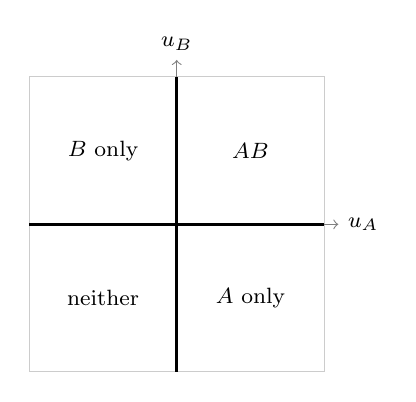
\begin{tikzpicture}[scale=0.72, font=\footnotesize]
  \draw[gray!40] (-2.6,-2.6) rectangle (2.6,2.6);
  \draw[->, gray] (-2.6,0) -- (2.85,0) node[right, black] {$u_A$};
  \draw[->, gray] (0,-2.6) -- (0,2.9) node[above, black] {$u_B$};
  \draw[very thick] (-2.6,0) -- (2.6,0);
  \draw[very thick] (0,-2.6) -- (0,2.6);
  \node at (1.3,1.3) {$AB$};
  \node at (1.3,-1.3) {$A$ only};
  \node at (-1.3,1.3) {$B$ only};
  \node at (-1.3,-1.3) {neither};
\end{tikzpicture}
\caption{$\Gamma_{AB} = 0$}
\end{subfigure}\hfill
\begin{subfigure}[b]{0.32\textwidth}
\centering
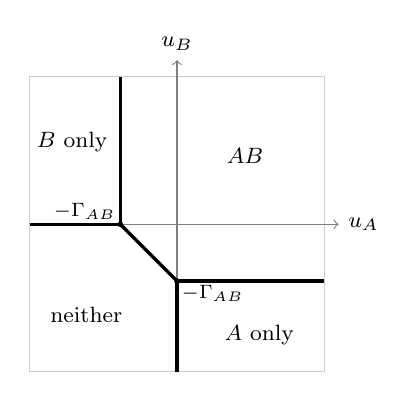
\begin{tikzpicture}[scale=0.72, font=\footnotesize]
  \draw[gray!40] (-2.6,-2.6) rectangle (2.6,2.6);
  \draw[->, gray] (-2.6,0) -- (2.85,0) node[right, black] {$u_A$};
  \draw[->, gray] (0,-2.6) -- (0,2.9) node[above, black] {$u_B$};
  \draw[very thick] (-2.6,0) -- (-1,0) -- (-1,2.6);
  \draw[very thick] (-1,0) -- (0,-1);
  \draw[very thick] (0,-2.6) -- (0,-1) -- (2.6,-1);
  \fill (-1,0) circle (1.4pt);
  \fill (0,-1) circle (1.4pt);
  \node[anchor=south east, inner sep=1.5pt] at (-1,0) {\scriptsize $-\Gamma_{AB}$};
  \node[anchor=north west, inner sep=1.5pt] at (0,-1) {\scriptsize $-\Gamma_{AB}$};
  \node at (1.2,1.2) {$AB$};
  \node at (1.45,-1.95) {$A$ only};
  \node at (-1.85,1.45) {$B$ only};
  \node at (-1.6,-1.6) {neither};
\end{tikzpicture}
\caption{$\Gamma_{AB} > 0$ (complements)}
\end{subfigure}\hfill
\begin{subfigure}[b]{0.32\textwidth}
\centering
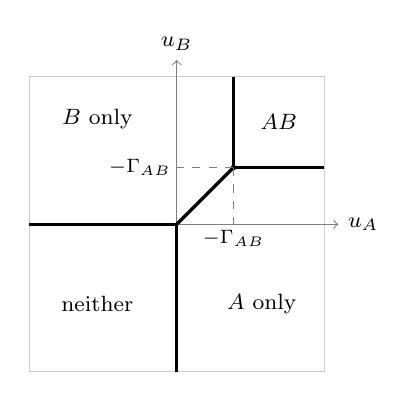
\begin{tikzpicture}[scale=0.72, font=\footnotesize]
  \draw[gray!40] (-2.6,-2.6) rectangle (2.6,2.6);
  \draw[->, gray] (-2.6,0) -- (2.85,0) node[right, black] {$u_A$};
  \draw[->, gray] (0,-2.6) -- (0,2.9) node[above, black] {$u_B$};
  \draw[very thick] (-2.6,0) -- (0,0) -- (0,-2.6);
  \draw[very thick] (0,0) -- (1,1);
  \draw[very thick] (1,2.6) -- (1,1) -- (2.6,1);
  \fill (1,1) circle (1.4pt);
  \draw[gray, dashed] (1,1) -- (1,0);
  \draw[gray, dashed] (1,1) -- (0,1);
  \node[anchor=north, inner sep=2pt] at (1,0) {\scriptsize $-\Gamma_{AB}$};
  \node[anchor=east, inner sep=2pt] at (0,1) {\scriptsize $-\Gamma_{AB}$};
  \node at (1.8,1.8) {$AB$};
  \node at (1.5,-1.4) {$A$ only};
  \node at (-1.4,1.85) {$B$ only};
  \node at (-1.4,-1.4) {neither};
\end{tikzpicture}
\caption{$\Gamma_{AB} < 0$ (substitutes)}
\end{subfigure}
\caption{Choice regions of the two-good bundle model in the plane of $(u_A, u_B)$, the utilities of $A$ and $B$ relative
to buying nothing. Thick lines are indifference boundaries. In panel (b) the anti-diagonal segment $u_A + u_B =
-\Gamma_{AB}$ separates buying both goods from buying neither. In panel (c) the diagonal segment $u_A = u_B$ separates
buying $A$ alone from buying $B$ alone. A rise in $p_B$ shifts probability mass downward. Only consumers on the
diagonal segments change their consumption of $A$. Drawn from the boundaries derived in the text. Compare
\citet[Figure~1]{Gentzkow2007}.}
\label{fig:10-gentzkow-regions}
\end{figure}

\casehead{Why the interaction term decides} A rise in $p_B$ lowers $u_B$ for every consumer and moves probability
mass down in \cref{fig:10-gentzkow-regions}. In panel (a), consumers who move from $AB$ to $A$ alone and from $B$
alone to nothing leave the demand for $A$ unchanged. In panel (b), some consumers on the anti-diagonal segment move
from $AB$ to nothing, so they stop buying $A$. In panel (c), consumers on the diagonal segment move from $B$ alone to
$A$ alone, so they start buying $A$ (pp.~718--719). The following result makes the argument exact.

\begin{proposition}[The interaction term signs the cross-price effect]\label{prop:10-gentzkow-subst}
In the model of \eqref{eq:10-gentzkow-twogood}, let $\alpha > 0$ and let $(\nu_A,\nu_B)$ have a continuous joint density that
is positive on $\R^2$. Write $f_u$ for the implied density of $(u_A, u_B)$. Then
\begin{equation}\label{eq:10-gentzkow-crossderiv}
  \frac{\partial Q_A}{\partial p_B} =
  \begin{cases}
    \alpha\displaystyle\int_0^{-\Gamma_{AB}} f_u(t,t)\,\dd t > 0 & \text{if } \Gamma_{AB} < 0,\\[2ex]
    0 & \text{if } \Gamma_{AB} = 0,\\[1ex]
    -\alpha\displaystyle\int_{-\Gamma_{AB}}^{0} f_u(-\Gamma_{AB} - t,\, t)\,\dd t < 0 & \text{if } \Gamma_{AB} > 0 .
  \end{cases}
\end{equation}
Hence $A$ and $B$ are substitutes if $\Gamma_{AB} < 0$, independent if $\Gamma_{AB} = 0$ and complements if
$\Gamma_{AB} > 0$ \citep[Proposition~1]{Gentzkow2007}.
\end{proposition}

\begin{proof}
\textit{Step 1: the condition for consuming $A$.} Ties have probability zero. The consumer consumes $A$ when her best
bundle containing $A$ beats her best bundle without it:
\begin{align*}
  \max\{u_A,\; u_A + u_B + \Gamma_{AB}\} &\ge \max\{0,\; u_B\}, \\
  u_A + \max\{0,\; u_B + \Gamma_{AB}\} &\ge \max\{0,\; u_B\}, \\
  u_A &\ge g(u_B), \qquad g(b) \equiv \max\{0, b\} - \max\{0, b + \Gamma_{AB}\} .
\end{align*}

\textit{Step 2: the shape of $g$.} If $\Gamma_{AB} = 0$, then $g \equiv 0$. If $\Gamma_{AB} > 0$, then $g(b) = 0$ for $b
\le -\Gamma_{AB}$, $g(b) = -\Gamma_{AB} - b$ for $-\Gamma_{AB} < b < 0$, and $g(b) = -\Gamma_{AB}$ for $b \ge 0$. So $g$ is
nonincreasing with slope $-1$ on $(-\Gamma_{AB}, 0)$. If $\Gamma_{AB} < 0$, then $g(b) = 0$ for $b \le 0$, $g(b) = b$ for
$0 < b < -\Gamma_{AB}$, and $g(b) = -\Gamma_{AB}$ for $b \ge -\Gamma_{AB}$. So $g$ is nondecreasing with slope $+1$ on
$(0, -\Gamma_{AB})$. Outside these intervals $g' = 0$.

\textit{Step 3: differentiate demand.} Write $c_A = \delta_A - \alpha p_A$ and $c_B = \delta_B - \alpha p_B$, so that
$u_A = c_A + \nu_A$ and $u_B = c_B + \nu_B$. Let $f$ be the density of $(\nu_A, \nu_B)$. Then
\begin{equation*}
  Q_A = \Pr\bigl(\nu_A \ge g(c_B + \nu_B) - c_A\bigr)
      = \int_{-\infty}^{\infty}\int_{g(c_B + \nu_B) - c_A}^{\infty} f(\nu_A, \nu_B)\,\dd\nu_A\,\dd\nu_B .
\end{equation*}
The function $g$ is piecewise linear, so we may differentiate under the outer integral:
\begin{align*}
  \frac{\partial Q_A}{\partial c_B} &= -\int_{-\infty}^{\infty} f\bigl(g(c_B + \nu_B) - c_A,\, \nu_B\bigr)\,
         g'(c_B + \nu_B)\,\dd\nu_B
      = -\int_{-\infty}^{\infty} f_u\bigl(g(t),\, t\bigr)\, g'(t)\,\dd t ,
\end{align*}
where the second equality substitutes $t = c_B + \nu_B$ and uses $f_u(a,b) = f(a - c_A, b - c_B)$. Since $\frac{\partial
c_B}{\partial p_B} = -\alpha$,
\begin{equation*}
  \frac{\partial Q_A}{\partial p_B} = \alpha\int_{-\infty}^{\infty} f_u\bigl(g(t),\, t\bigr)\, g'(t)\,\dd t .
\end{equation*}

\textit{Step 4: evaluate.} If $\Gamma_{AB} = 0$, then $g' \equiv 0$ and the derivative is zero. If $\Gamma_{AB} < 0$, then
$g(t) = t$ and $g'(t) = 1$ on $(0, -\Gamma_{AB})$, which gives the first line of \eqref{eq:10-gentzkow-crossderiv}. If
$\Gamma_{AB} > 0$, then $g(t) = -\Gamma_{AB} - t$ and $g'(t) = -1$ on $(-\Gamma_{AB}, 0)$, which gives the third line.
The density is positive, so both integrals are strictly positive.
\end{proof}

The two integrals run along the diagonal segments of \cref{fig:10-gentzkow-regions}. Gentzkow's equation~(3) writes
them as line integrals with indicator functions (p.~719). The magnitude of the cross effect depends on the length
$|\Gamma_{AB}|$ of the segment and on the density of consumers along it. The proposition also covers nonprice shifters.
Suppose a variable $z$ raises $u_B$ by $\zeta z$ and leaves $u_A$ unchanged. Then $\frac{\partial Q_A}{\partial z} =
\zeta\frac{\partial Q_A}{\partial c_B} = -\frac{\zeta}{\alpha}\frac{\partial Q_A}{\partial p_B}$. Improving the
connection speed of an online paper works like cutting its price, and its effect on print demand has the sign of
$\Gamma_{AB}$ (p.~719). This is how Gentzkow's excluded variables reveal substitution without any price variation.

\subsection{What the data can and cannot identify}\label{sec:10-gentzkow-ident}

\casehead{A counting problem} Choice data in the two-good model give three probabilities, $P_A$, $P_B$ and $P_{AB}$.
The model has five parameters: $\delta_A$, $\delta_B$, $\Gamma_{AB}$, $\rho$ and $\alpha$ (p.~720). The price
coefficient is identified from choices only if prices vary, because the probabilities depend on $(\delta_A, \delta_B,
\alpha)$ only through $\delta_A - \alpha p_A$ and $\delta_B - \alpha p_B$. Without price variation, $\alpha$ needs
another moment. Gentzkow takes it from a firm's pricing condition (\cref{sec:10-gentzkow-supply}).

The harder problem is to separate $\Gamma_{AB}$ from $\rho$. The marginal probabilities $Q_A$ and $Q_B$ identify the two
mean utilities. One moment remains, how often the goods are consumed together. A high $P_{AB}$ relative to $P_A$ and
$P_B$ can come from a large $\Gamma_{AB}$ or from a large $\rho$, and nothing else in the data separates them
(p.~720). By \cref{prop:10-gentzkow-subst}, the same data could be fit by near-perfect substitutes with highly
correlated tastes, or by near-perfect complements with weakly correlated tastes. A model that fixes one of the two
parameters by assumption fixes the answer to the substitution question.

\casehead{Exclusion restrictions} Suppose a variable $x$ enters the utility of $A$ only. Observing choices at a second
value of $x$ adds three moments, $P_A$, $P_B$ and $P_{AB}$ at the new value, and one parameter, the new mean utility of
$A$ (p.~721). The model becomes formally identified. The intuition is direct. If joint consumption reflects a high
$\Gamma_{AB}$, then shifting up the utility of $A$ raises the probability of consuming $B$. If it reflects correlated
tastes, the probability of consuming $B$ stays unchanged. \citet{Keane1992} gives Monte Carlo evidence that exclusion
restrictions sharpen the covariance estimates of multinomial probit models, which nest the model of \eqref{eq:10-gentzkow-twogood}
when defined over bundles (p.~721, n.~11).

\casehead{Panel data} Split each taste into a consumer random effect, constant over time, and a shock that is \iid\
across goods and days. With choices observed at two dates there are $4^2 = 16$ joint outcomes, hence 15 moments
instead of 3 (p.~721, n.~12). The argument is the usual one for random effects. Correlated random effects make some
consumers likely to consume both goods and others likely to consume neither. Conditional on a consumer's average
propensities, her day-to-day variation is then uncorrelated across goods. A high $\Gamma_{AB}$ instead makes the
day-to-day variation strongly correlated. The consumer reads both papers on some days and neither on others, and
rarely reads only one.

Gentzkow's data are a limited panel. Respondents report what they read in the last 24 hours and in the last five
weekdays. For consumers who read nothing in the last 24 hours, the five-day report shows which papers they read on
the other four weekdays. Whether they
were less likely to read then identifies the variance of the random effects. Consumers who read one paper in the last
24 hours identify the correlation. If the random effects are positively correlated, a consumer who read only $A$
yesterday is more likely to have read $B$ earlier in the week (p.~722).

\casehead{Unobserved goods} The outside option has a different meaning when bundles are allowed. Every choice in the
model includes an implicit maximization over goods the econometrician does not see, such as cable news (p.~719).
Suppose watching CNN destroys the value of the post.com and raises the value of the print \textit{Post}. Then the
\textit{Post} and the post.com are never read together, and the model estimates them as strong substitutes. Gentzkow
argues that this answer is correct for the market as it is. Raising the price of the \textit{Post} would reduce CNN
viewing as well and raise post.com reading (p.~720). The estimates are conditional on the set and the prices of the
unobserved goods, a limitation all discrete choice models share \citep{Samuelson1974}.

\casehead{Relation to earlier models} The model of \eqref{eq:10-gentzkow-twogood} nests the earlier approaches as restrictions
(pp.~722--723). The multiple-discrete choice model of \citet{Hendel1999} aggregates many ``tasks,'' such as the
computing needs of each employee of a firm. Hendel's model lets a buyer choose several units of several brands, and he
estimates it by the method of simulated moments on micro data for personal computer purchases by firms. Each task uses
one good, so the task-level model fixes $\Gamma_{AB} = -\infty$, and the goods are restricted to be substitutes
(\cref{ch:logit}). A multivariate probit, with one equation per good and correlated errors, sets $\Gamma_{AB} = 0$
and forces independence. A logit or nested logit over bundles \citep{ManskiSherman1980,TrainMcFaddenBenAkiva1987} can
estimate $\Gamma_{AB}$ freely. Its unobservables, however, are uncorrelated or follow the nest structure, so it would
read correlated tastes as complementarity. Gentzkow's model frees both terms and relies on exclusions and panel
information to separate them.

\subsection{Setting and data}\label{sec:10-gentzkow-data}

The data come from a Scarborough Research survey of 16,179 adults in the Washington, DC, Designated Market Area (DMA),
conducted between March 2000 and February 2003 (p.~723). The survey lists the local print newspapers each respondent
read in the last 24 hours and in the last five weekdays. It records the readership of the major local online newspapers
over the same windows, and many household characteristics. The \textit{Post} dominated the market, with an average daily readership
of 1.8 million against 256,000 for the \textit{Times}. The post.com had 406,000 area readers per day. The
\textit{Times}'s own website had only 373 readers in the sample and is omitted (p.~723, n.~16). The goods are the daily
editions of the \textit{Post}, the \textit{Times} and the post.com. The outside option includes all other news
sources and not reading news at all.

The survey is about a 0.4 percent sample and broadly representative. It overrepresents older, more educated and
wealthier residents and underrepresents minorities (p.~724). Estimation uses the unweighted data, and the policy
simulations use the sampling weights. About 6 percent of records were filled in by Scarborough from matched
respondents. Gentzkow drops them in estimation and keeps them in the simulations (p.~724, n.~17).

The aggregate time series are suggestive but inconclusive (p.~724). Post.com readership grew rapidly after its
introduction in 1996 while \textit{Post} readership fell. A regression of \textit{Post} readership since 1984 on
post.com readership and a trend implies that four post.com readers displace one \textit{Post} reader. Yet the decline
began in 1994, two years before the post.com, and did not accelerate afterward. Readership was falling nationally, and
the \textit{Post} raised its subscription price several times. Time series alone cannot separate these forces.

The micro data show that reading several papers is common (p.~725). Forty-eight percent of respondents read at least
one of the three papers in the last 24 hours. Of these, 18 percent read two and 1 percent read all three. Over five
days, 65 percent read at least one, and of these 27 percent read two and 3 percent all three. Panel~A of
\cref{tab:10-gentzkow-data} cross-tabulates \textit{Post} and post.com readership. Among post.com readers the share who
also read the \textit{Post} is higher than among non-readers. Panel~B reports raw and partial correlations. The partial
correlations control for age, sex, education, occupation, employment status, income, political party, survey date,
location and the number of missing answers. Controls cut the \textit{Post}-post.com correlation by about two-thirds,
but it stays significantly positive. The \textit{Post}-\textit{Times} correlation is positive in the raw data and
vanishes or turns negative with controls.

\begin{table}[htbp]
\centering
\caption{Joint readership of the \textit{Post}, the post.com and the \textit{Times}}\label{tab:10-gentzkow-data}
\small
\begin{tabular}{@{}lrrrr@{}}
\toprule
\multicolumn{5}{@{}l}{\textit{A. Cross-tabulation of Post and post.com readership (number of respondents)}} \\
 & \multicolumn{2}{c}{Last 24 hours} & \multicolumn{2}{c}{Last 5 weekdays} \\
\cmidrule(lr){2-3}\cmidrule(l){4-5}
 & No post.com & Read post.com & No post.com & Read post.com \\
\midrule
Did not read \textit{Post} & 8,771 & 622 & 6,012 & 680 \\
Read \textit{Post}         & 5,829 & 877 & 7,203 & 2,204 \\
\midrule
\multicolumn{5}{@{}l}{\textit{B. Correlation coefficients of readership indicators}} \\
 & \multicolumn{2}{c}{Last 24 hours} & \multicolumn{2}{c}{Last 5 weekdays} \\
\cmidrule(lr){2-3}\cmidrule(l){4-5}
 & Raw & Partial & Raw & Partial \\
\midrule
\textit{Post} and post.com        & 0.0989$^{**}$ & 0.0364$^{**}$ & 0.1579$^{**}$ & 0.0673$^{**}$ \\
\textit{Post} and \textit{Times}  & 0.0632$^{**}$ & 0.0035        & 0.0450$^{**}$ & $-0.0623^{**}$ \\
\textit{Times} and post.com       & 0.0146        & 0.0090        & 0.0184        & 0.0066 \\
\bottomrule
\end{tabular}

\smallskip
\begin{minipage}{0.92\textwidth}
\footnotesize Source: \citet[Tables~2 and 3]{Gentzkow2007}, Scarborough survey, Washington, DC, DMA, 2000--03.
Partial correlations are correlations of the residuals from regressions of each readership indicator on the controls
listed in the text. Panel~B drops respondents for whom print or online papers are not in the choice set.
$^{**}$ significant at 1 percent.
\end{minipage}
\end{table}

\subsection{Reduced-form evidence}\label{sec:10-gentzkow-reduced}

To separate complementarity from correlated tastes, Gentzkow uses four variables that shift the utility of reading
online but not, directly, the utility of reading print (pp.~725--726). They are indicators for Internet access at work,
use of the Internet for work-related tasks, use of the Internet for education-related tasks, and a high-speed
connection at home. Access at work lowers the time cost of reading online. The two use variables indicate familiarity
with the Internet and time spent at a computer. A fast connection raises the utility of online reading. Collect them
in a vector $z_i$. No variable shifts the \textit{Post} without shifting the \textit{Times}, so print-print
substitution is less well identified than print-online substitution (p.~726).

A linear probability model shows the exclusion restrictions at work. Let $R^p_i$ indicate that respondent $i$ read the
\textit{Post} in the last five weekdays and $R^w_i$ that she read the post.com. Gentzkow estimates
\begin{equation}\label{eq:10-gentzkow-lpm}
  R^p_i = b\,R^w_i + x_i\varphi + e_i ,
\end{equation}
first by OLS and then by two-stage least squares (2SLS) with $z_i$ as instruments for $R^w_i$. The controls $x_i$ are
those of the partial correlations, plus \textit{Times} readership. The 2SLS coefficient has a simple interpretation in
terms of \cref{prop:10-gentzkow-subst}. Each instrument moves only the utility of the post.com, so it acts like a change
in the post.com's price. The 2SLS coefficient is the ratio of the instrument's effect on \textit{Post} reading to its
effect on post.com reading. In the language of \cref{ch:diffprod}, it estimates minus the diversion ratio from the
post.com to the \textit{Post}, averaged over the respondents whom the instruments move.

\Cref{tab:10-gentzkow-lpm} reproduces Table~4. OLS gives a positive coefficient, 0.0464 (0.0090), which mirrors the
raw correlation. 2SLS gives $-0.4132$ (0.107). Taken literally, a respondent assigned to read the online paper at zero
time cost would be about 41 percentage points less likely to read the print paper. Gentzkow describes this as
``40 percent less likely'' (p.~726). The coefficient on a binary regressor in a linear probability model is a change
in the probability itself. A relative decline would require dividing by a baseline probability of reading the
print paper. Gentzkow warns that the linear
probability model limits how far this magnitude can be trusted. The first-stage $F$-statistic on the instruments is
33.05, so weak instruments are not a concern. The overidentification statistic is $\chi^2 = 3.65$ with a $p$-value of
0.302, so the test does not reject the validity of the instruments.

\begin{table}[htbp]
\centering
\caption{Linear probability model of \textit{Post} readership in the last five weekdays}\label{tab:10-gentzkow-lpm}
\small
\begin{tabular}{@{}lcccc@{}}
\toprule
 & OLS & \multicolumn{3}{c}{2SLS} \\
\cmidrule(l){3-5}
 &  & (1) & (2) & (3) \\
\midrule
Read post.com last 5 days & 0.0464$^{**}$ & $-0.4132^{**}$ & $-0.4579^{**}$ & $-0.4381^{**}$ \\
                          & (0.0090)      & (0.107)        & (0.119)        & (0.141) \\
Other Internet news       &               &                &                & 0.0244 \\
                          &               &                &                & (0.0195) \\
Industry and occupation controls &        &                & Yes            &  \\
Overidentification $p$-value &            & 0.302          & 0.431          & 0.219 \\
$R^2$                     & 0.333         & 0.214          & 0.207          & 0.202 \\
$N$                       & 14,313        & 14,313         & 14,313         & 14,313 \\
\bottomrule
\end{tabular}

\smallskip
\begin{minipage}{0.92\textwidth}
\footnotesize Source: \citet[Table~4]{Gentzkow2007}. Robust standard errors in parentheses. The instruments are
indicators for Internet access at work, a fast Internet connection, and use of the Internet for research or education
and for work. The overidentification test is a Sargan test. Industry controls are 12 categories and occupation
controls 11. All regressions include the controls listed in the text and omit respondents without print papers in the
choice set. $^{**}$ significant at 1 percent.
\end{minipage}
\end{table}

The main threat is that the instruments correlate with unmeasured tastes for print (pp.~727--728). People who like
reading may select into jobs with Internet access, and news enthusiasts may buy fast connections. Gentzkow offers three
checks. Adding 12 industry and 11 occupation categories, which should absorb part of any omitted job characteristic,
strengthens the 2SLS coefficient slightly to $-0.4579$ \citep{AltonjiElderTaber2005}. Restricting the sample to
residents of more than ten years, whose job choices largely predate online news, leaves the estimates nearly unchanged
(p.~727, n.~19). Controlling for other Internet news use raises the coefficient's magnitude slightly ($-0.4381$), so the
instruments do not appear to work through other online news sources. The structural robustness checks below also drop
the broadband exclusion.

\subsection{The empirical model}\label{sec:10-gentzkow-structural}

Index days by $t$, consumers by $i$, goods by $j \in \{1, \dots, J\}$ with $J = 3$, and bundles by $r \in \{0, 1, \dots,
2^J - 1\}$, where $r = 0$ is the empty bundle (p.~728). The utility of consumer $i$ from good $j$ alone on day $t$ is
\begin{equation}\label{eq:10-gentzkow-base}
  \tilde u_{ijt} = \delta_j - \alpha p_j + x_i\beta_j + \nu_{ij} + \tau_{it} .
\end{equation}
The vector $x_i$ holds age, sex, education, occupation, employment status, political party, location within the DMA,
the number of missing survey answers, six-month time dummies and log income. For the post.com it also holds the four
excluded variables $z_i$, which are absent from the print utilities. The time dummies absorb changes in the quality of
the goods and their substitutes. Log income proxies for unobservables correlated with income, since the budget effect
of income differences out (p.~729).

The two unobservables play different roles. The vector $\nu_i = (\nu_{i1}, \dots, \nu_{iJ})$ is constant over the
survey week. It captures a general taste for news, loyalty to a paper and subscription status. It is multivariate
normal with a free covariance matrix, whose scale is pinned down by the logit errors below (p.~729, n.~21). The day
shock $\tau_{it}$ raises the utility of all papers equally. It equals $\hat\tau > 0$ with probability $\varpi$ and zero
otherwise, a stylized description of major news days and of day-to-day variation in the cost of time. Price does not
vary enough to estimate $\alpha$ from demand, so the first two terms are combined into $\bar\delta_j = \delta_j - \alpha
p_j$.

The utility of bundle $r$ adds the base utilities of its goods, an interaction term and a bundle-specific shock
(p.~729, eq.~4):
\begin{equation}\label{eq:10-gentzkow-bundle}
  u_{irt} = \begin{cases}
    \epsilon_{irt} & \text{if } r = 0, \\
    \sum_{j \in r}\tilde u_{ijt} + \Gamma_r + \epsilon_{irt} & \text{if } r > 0.
  \end{cases}
\end{equation}
Here $\Gamma_r = 0$ for single-good bundles, and $\epsilon_{irt}$ is \iid\ type-I extreme value. With three goods there
are three pairwise interactions and one triple interaction, which is estimated but not reported (Table~6, note). On a
major news day the bundle $r$ gains $|r|\hat\tau$, where $|r|$ is its number of goods. The interaction terms and the
price coefficient are common to all consumers. Gentzkow reports that letting $\Gamma_r$ vary with observables did not
change the results substantially (p.~729).

\Cref{prop:10-gentzkow-subst} does not apply unchanged to this model. Label the goods $A$, $B$ and $C$. With three
goods, a change in $p_B$ also moves consumers into and out of the bundles that contain $C$. The triple interaction
and the bundle-specific logit errors then enter the cross-price effect, and a negative $\Gamma_{AB}$ no longer
signs it. Our computation gives an example with $\nu_i$ and $\tau_{it}$ set to zero. Let every
$\bar\delta_j + x_i\beta_j$ be zero, $\alpha = 1$, $\Gamma_{AB} = -1$, $\Gamma_{AC} = \Gamma_{BC} = 0$, and
$\Gamma_r = 10$ for the bundle $r$ of all three goods. With $r_i$ the bundle that consumer $i$ chooses, the logit form
gives $\frac{\partial Q_A}{\partial p_B} = -\alpha\Cov\bigl(\indic\{A\in r_i\},\indic\{B\in r_i\}\bigr) \approx -0.00009$.
So $A$ and $B$ are complements although $\Gamma_{AB} < 0$, because almost every consumer buys all three goods. A
small positive variance of $\nu_i$ preserves the sign. In the empirical model the two-good result is therefore an
intuition, and the substitution patterns must be read from the cross-price derivatives of the full model.

Two dummies define choice sets. About 10 percent of respondents say they look at no newspaper sections, and print
papers are removed from their choice set. Respondents who did not use the Internet in the last 30 days have no online
paper. Each dummy also enters, as a control, the utility of the goods it does not exclude (p.~729). Choice-set
variation therefore does not identify substitution, which seems prudent because it is unlikely to be exogenous
(n.~25).

\casehead{Choice probabilities and the likelihood} Integrating over the $\epsilon_{irt}$ gives the logit probability of
bundle $r$ on a day with shock $\tau$:
\begin{equation}\label{eq:10-gentzkow-Q}
  Q_r(x_i, \nu_i, \tau; \theta) = \frac{\exp\Bigl[\sum_{j\in r}(\bar\delta_j + x_i\beta_j + \nu_{ij} + \tau) + \Gamma_r\Bigr]}
  {1 + \sum_{r'=1}^{2^J - 1}\exp\Bigl[\sum_{j\in r'}(\bar\delta_j + x_i\beta_j + \nu_{ij} + \tau) + \Gamma_{r'}\Bigr]} .
\end{equation}
The data report, for each good, whether it was read in the last 24 hours and whether it was read in the last five
weekdays. Let $\tilde q \in \{0, \dots, 2^J - 1\}^5$ list the bundles chosen on the five weekdays. Let $q$ be a reported
outcome and $\Omega(q)$ the set of daily sequences consistent with it. Since $\tau_{it}$ and $\epsilon_{irt}$ are
independent across days, the probability of report $q$ given $\nu_i$ is (p.~730)
\begin{equation}\label{eq:10-gentzkow-Pq}
  P_q(x_i, \nu_i; \theta) = \sum_{\tilde q \in \Omega(q)}\prod_{t=1}^{5}\Bigl[\varpi\,Q_{\tilde q_t}(x_i, \nu_i, \hat\tau;
  \theta) + (1 - \varpi)\,Q_{\tilde q_t}(x_i, \nu_i, 0; \theta)\Bigr] .
\end{equation}
The log-likelihood integrates over the random effects:
\begin{equation}\label{eq:10-gentzkow-loglik}
  L(X, q, \theta) = \sum_i \ln\int P_{q_i}(x_i, \nu; \theta)\,\dd F(\nu; \theta),
\end{equation}
where $F(\nu; \theta)$ is the multivariate normal distribution of $\nu$ (p.~732, eq.~6).

\casehead{Identification in the empirical model} The two-good intuition carries over (p.~730). The combination of
24-hour and 5-day reports pins down the covariance matrix of $\nu_i$. Choices on earlier days are more correlated with
the choice in the last 24 hours, conditional on observables, the larger the variance of the random effects. The
exclusion restrictions then pin down the distribution of the common day shock $\tau_{it}$ and the interaction terms. If
same-day joint reading of print and online papers is driven by $\tau_{it}$, Internet access at work should not change
the probability of reading print. If it is driven by complementarity, those with access should read print more.
Gentzkow stresses three limitations. The partial panel identifies the random effects less well than a true panel.
The excluded variables shift only the online paper. And without price variation, functional forms carry more weight
than in richer data sets.

\subsection{Simulated maximum likelihood}\label{sec:10-gentzkow-sml}

The integral in \eqref{eq:10-gentzkow-loglik} has no closed form. Gentzkow replaces it with a simulator and maximizes
the simulated likelihood (p.~732, eq.~7):
\begin{equation}\label{eq:10-gentzkow-sml}
  \hat\theta^{SML} = \argmax_\theta \sum_i \ln\Bigl[\frac{1}{S}\sum_{s=1}^{S}P_{q_i}(x_i, \nu_{is}; \theta)\Bigr],
\end{equation}
with $S = 300$ draws per consumer. The leading alternative is the method of simulated moments (MSM) of
\citet{McFadden1989} and \citet{PakesPollard1989}. MSM is consistent for a fixed number of draws. Simulated maximum
likelihood (SML), introduced by \citet{LermanManski1981}, needs the number of draws to grow with the sample
\citep{GourierouxMonfort1996}. But efficient MSM requires optimal instruments, which perform poorly when the
preliminary estimate is inaccurate, and it requires the probabilities of all possible reports. With many reported
outcomes this is expensive. In preliminary tests the two estimators gave similar parameters, and MSM took 10 to 20 times
longer, so Gentzkow uses SML (p.~732).

\casehead{Importance sampling} Draws from the unconditional distribution of $\nu$ waste effort on values that make the
observed report unlikely. Gentzkow instead draws from the distribution of $\nu$ conditional on the observed report,
computed at a preliminary estimate $\tilde\theta$ (p.~732, n.~31). The logic is clearest when the draws are standardized
shocks $\eta \sim N(0, I)$ with density $\phi$, and $\nu = C(\theta)\eta$. (In this subsection $\eta$ and $\phi$
denote these shocks and their density, not the CES elasticity of \cref{sec:10-feenstra}.) Write $P_i(\eta; \theta) \equiv
P_{q_i}(x_i, C(\theta)\eta; \theta)$ for the probability of $i$'s report given the shocks. Let $\bar P_i(\tilde\theta) = \int
P_i(\eta; \tilde\theta)\phi(\eta)\,\dd\eta$, computed once with many draws. The importance density is
\begin{equation*}
  h_i(\eta) = \frac{P_i(\eta; \tilde\theta)\,\phi(\eta)}{\bar P_i(\tilde\theta)} ,
\end{equation*}
which is the posterior density of $\eta$ given the report. The weighted simulator
\begin{equation*}
  \tilde P_i(\theta) = \frac{1}{S}\sum_{s=1}^{S}P_i(\eta_s; \theta)\,W_{is}, \qquad
  W_{is} = \frac{\bar P_i(\tilde\theta)}{P_i(\eta_s; \tilde\theta)}, \qquad \eta_s \sim h_i,
\end{equation*}
is unbiased for every $\theta$:
\begin{equation*}
  \E_h\bigl[P_i(\eta; \theta)\,W_i\bigr]
  = \int P_i(\eta; \theta)\,\frac{\bar P_i(\tilde\theta)}{P_i(\eta; \tilde\theta)}\,
    \frac{P_i(\eta; \tilde\theta)\,\phi(\eta)}{\bar P_i(\tilde\theta)}\,\dd\eta
  = \int P_i(\eta; \theta)\,\phi(\eta)\,\dd\eta .
\end{equation*}
Draws from $h_i$ are taken by acceptance and rejection, since $h_i$ is the distribution of the shocks conditional on the
observed report. \emph{Acceptance and rejection} draws $\eta$ from $\phi$ and keeps each draw with probability
proportional to $P_i(\eta;\tilde\theta)$, so the kept draws follow $h_i$. Gentzkow writes the same simulator in terms of $\nu$ (his eqs.~13--14). The general treatment of
importance sampling is in \cref{sec:08-importance}.

\casehead{Bias correction} SML is biased in finite samples because the logarithm is concave (p.~732, n.~32). Let
$\tilde f$ be an unbiased simulator of a choice probability $f$, so $\E\tilde f = f$. A second-order expansion of $\ln
\tilde f$ around $f$ gives
\begin{align*}
  \ln\tilde f &= \ln f + \frac{\tilde f - f}{f} - \frac{(\tilde f - f)^2}{2f^2} + O\bigl(|\tilde f - f|^3\bigr), \\
  \E\ln\tilde f &\approx \ln f - \frac{1}{2}\,\frac{\E(\tilde f - f)^2}{f^2} = \ln f - \frac{1}{2}\,\frac{\Var(\tilde f)}{f^2} .
\end{align*}
The expected simulated log-likelihood is too low by about half the squared coefficient of variation of the simulator.
If $\tilde f = \frac{1}{S}\sum_s P_{is}$ averages $S$ independent draws, then $\Var(\tilde f) = \frac{1}{S}\Var(P_{is})$,
which can be estimated by $\frac{1}{S^2}\sum_s(P_{is} - \tilde f)^2$. The corrected objective adds this estimate back:
\begin{equation}\label{eq:10-gentzkow-biascorr}
  \hat\theta = \argmax_\theta\sum_i\Biggl\{\ln\tilde f_i + \frac{1}{2}\,
  \frac{\frac{1}{S^2}\sum_{s}\bigl(P_{is} - \tilde f_i\bigr)^2}{\tilde f_i^2}\Biggr\} .
\end{equation}
The correction removes the bias of order $\frac{1}{S}$ \citep[p.~45]{GourierouxMonfort1996}.\footnote{The version of
\eqref{eq:10-gentzkow-biascorr} printed in Gentzkow's footnote 32 does not show the factor $\frac{1}{S^2}$ in the
correction term. We state the expression that follows from the expansion.} The robust standard errors follow
\citet{McFaddenTrain2000}. For welfare and other derived statistics, Gentzkow draws 100 parameter vectors from the
estimated asymptotic distribution, recomputes the statistic at each, and reports the standard deviation (p.~733). This
avoids the delta method, which linearizes highly nonlinear functions.

\subsection{The price coefficient from the supply side}\label{sec:10-gentzkow-supply}

Demand data identify only $\bar\delta_j = \delta_j - \alpha p_j$. To express utility in dollars, Gentzkow backs out
$\alpha$ from the condition that the \textit{Post} sets its print price optimally (pp.~730--731 and 735--736). The idea
is that the less price-sensitive consumers are, the higher the price a profit-maximizing firm would set (p.~715).

\casehead{Profit} The \textit{Post} sells copies at price $p$, and each copy is read by $\kappa$ adults. The firm
earns advertising revenue $a_p$ per print reader and $a_w$ per online reader, pays marginal cost $c_p$ per printed copy,
and bears a fixed cost. With $N_p$ print readers and $N_w$ online readers, the profit of the Washington Post Company is
(p.~731, eq.~5)
\begin{equation}\label{eq:10-gentzkow-profit}
  \Pi = \Bigl[a_p + \frac{p - c_p}{\kappa}\Bigr]N_p + a_w N_w - F^{\mathrm{fix}} .
\end{equation}
The marginal cost of an extra online reader is taken to be zero, and advertising revenue per reader is constant. The
second assumption treats both advertising markets as competitive at a fixed price per reader. It abstracts from the
different values of different readers and from any market power of the \textit{Post} (p.~735). Since $\kappa$ readers
share each copy, Gentzkow assumes that each reader pays $\frac{p}{\kappa}$ and that this reader price enters the
utility \eqref{eq:10-gentzkow-base} (p.~731).

\casehead{Inputs} Every input comes from industry data (pp.~735--736).
\begin{itemize}
  \item Print advertising revenue was \$574.3 million in 2001 and \$555.7 million in 2002. The daily edition's share
        gives \$1.5 and \$1.4 million per day, and with daily circulation of 771,614 and 768,600 the average is $a_p =
        \$1.91$.
  \item Online division revenue was \$30.4 million in 2001 and \$35.9 million in 2002. The post.com had 450,457 daily
        readers in the DMA, about 75 percent of its total. Dividing 75 percent of revenue by DMA readership gives
        $a_w = \$0.15$. A second estimate from the advertising revenue and readership of nytimes.com gives \$0.16,
        which Gentzkow uses.
  \item Newsprint consumption of 226,796 metric tons at \$541 per ton implies \$0.37 per copy. With ink and distribution,
        $c_p = \$0.40$.
  \item The cover price rose from \$0.25 to \$0.35 over the period, and the subscription price per daily copy was
        \$0.22 to \$0.25. Gentzkow uses $p = \$0.30$.
  \item Comparing survey readership with audited circulation gives $\kappa = 2.4$ readers per copy (2.3 for the
        \textit{Times}). Whether $\kappa$ reflects shared copies or overreporting does not change the welfare results
        (p.~731, n.~28).
\end{itemize}
The profit from one more print reader is \$0.75, and from one more online reader \$0.16 (p.~736).\footnote{With the
reported inputs, $\frac{a_p + p - c_p}{\kappa} = \frac{1.91 + 0.30 - 0.40}{2.4} = 0.754$, which reproduces the \$0.75
in the paper. The bracket of \eqref{eq:10-gentzkow-profit} as printed, $a_p + \frac{p - c_p}{\kappa}$, would give about
\$1.87. The reported figure is therefore consistent with $a_p$ measured per copy, which is how it is computed from
circulation.}

\casehead{The first-order condition} Write the expected numbers of print and online readers as functions $N_p(\bar
\delta; \hat\theta)$ and $N_w(\bar\delta; \hat\theta)$ of the vector of constants $\bar\delta$ and the other estimated
parameters $\hat\theta$. These and their derivatives are computed by simulation. Let $m_p$ denote the profit per print
reader. Using $\frac{\partial\bar\delta_j}{\partial p_j} = -\alpha$ as Gentzkow does, the derivative of \eqref{eq:10-gentzkow-profit}
with respect to the print price is (p.~736)
\begin{equation}\label{eq:10-gentzkow-foc}
  \frac{\partial\Pi}{\partial p} = -\alpha\Bigl[m_p\frac{\partial N_p}{\partial\bar\delta_{\mathrm{post}}}
  + a_w\frac{\partial N_w}{\partial\bar\delta_{\mathrm{post}}}\Bigr] + \frac{1}{\kappa}N_p = 0 .
\end{equation}
Everything except $\alpha$ is known. Solving,
\begin{equation}\label{eq:10-gentzkow-alpha}
  \hat\alpha = \frac{N_p}{\kappa\Bigl[m_p\frac{\partial N_p}{\partial\bar\delta_{\mathrm{post}}}
  + a_w\frac{\partial N_w}{\partial\bar\delta_{\mathrm{post}}}\Bigr]} ,
\end{equation}
which is unique whenever the bracket is nonzero. Gentzkow obtains $\hat\alpha = 9.72$ (p.~736). As in Gentzkow's
equation, $\alpha$ here is the coefficient on the copy price $p$. If utility depends instead on the reader price
$\frac{p}{\kappa}$, the coefficient on that price is $\kappa\alpha$. Utils then convert into dollars at that rate
\citep[n.~28]{Gentzkow2007}. The elasticity \eqref{eq:10-gentzkow-lerner} below is the same under either
convention.

The condition has a transparent economic reading. A higher $\bar\delta_{\mathrm{post}}$ raises print readership,
$\frac{\partial N_p}{\partial\bar\delta_{\mathrm{post}}} > 0$, and lowers online readership when the goods are
substitutes. Define the diversion ratio $D = -\frac{\partial N_w}{\partial\bar\delta_{\mathrm{post}}}
\bigl(\frac{\partial N_p}{\partial\bar\delta_{\mathrm{post}}}\bigr)^{-1}$ and the price elasticity of print readership $\varepsilon_p = -\frac{\partial
N_p}{\partial p}\frac{p}{N_p}$. Rearranging \eqref{eq:10-gentzkow-foc} gives
\begin{equation}\label{eq:10-gentzkow-lerner}
  \varepsilon_p = \frac{\frac{p}{\kappa}}{m_p - a_w D} .
\end{equation}
The price paid per reader, $\frac{p}{\kappa} = \$0.125$, is far below the profit per reader, \$0.75, because each reader
brings advertising revenue. The \textit{Post} therefore prices where its demand is inelastic. By the chain rule,
$\varepsilon_p = \alpha\,p\,\frac{\partial N_p}{\partial\bar\delta_{\mathrm{post}}}\frac{1}{N_p}$, and the estimated
demand parameters fix the readership response $\frac{\partial N_p}{\partial\bar\delta_{\mathrm{post}}}$ and $N_p$. With
these and $p$ held fixed, the elasticity is proportional to $\alpha$, so a low elasticity requires a small $\alpha$.
A price change then moves utility little relative to the spread of the taste shocks. The paper reports an implied own-price elasticity of
0.37 and finds that it tracks the \textit{Post}'s readership response to its price increases over 1994--2003 (p.~738,
n.~38).\footnote{Inserting the reported inputs into \eqref{eq:10-gentzkow-lerner} gives an elasticity between 0.17 (at
$D = 0$) and 0.21 (at $D = 1$). The paper does not show how its elasticity of 0.37 is computed, so we cannot locate the
source of the gap.}
The strategy rests on strong assumptions. The print price must be optimal given the zero online price, the advertising
model must be right, and the cost data must be accurate. Gentzkow shows in \cref{tab:10-gentzkow-robust} that the
qualitative results survive reasonable changes in $p$, $c_p$ and $a_w$.

\subsection{Results: demand parameters and substitution}\label{sec:10-gentzkow-results}

\casehead{Observables} \Cref{tab:10-gentzkow-obs} reproduces Table~5, the coefficients on consumer characteristics in
the mean utility of each good (p.~733). Most coefficients for the \textit{Post} and the post.com are significant, as
are about half of those for the \textit{Times}. Gentzkow reads them through marginal effects on the probability of
reading each paper, for a consumer at the mean of the data. The \textit{Post} fits its reputation as a high-brow,
liberal paper. Attending college, attending graduate school and doubling household income raise the probability of
reading the \textit{Post} by 31, 34 and 9 percentage points. Being a registered Democrat raises it by 3 points, and being a registered Republican
lowers it by 2. Ten more years of age add 8 points, while full-time employment lowers the probability by 14 points.
The post.com's coefficients mostly share the \textit{Post}'s signs, with smaller marginal effects because its predicted
probability is lower (16 percent against 53). Age and employment are exceptions. Ten more years of age lower the
probability of reading the post.com by 1 point, and full-time work, white-collar work and computer work raise it by 2,
1 and 3 points. The online edition is often read at work and draws younger readers (p.~734). Registered
Republicans are 3 points more likely to read the \textit{Times}, whose mean predicted probability is 9 percent (p.~734).

\begin{table}[htbp]
\centering
\caption{Gentzkow's estimates of the effects of consumer characteristics on utility}\label{tab:10-gentzkow-obs}
\small
\begin{tabular}{@{}lccc@{}}
\toprule
 & \textit{Post} & post.com & \textit{Times} \\
\midrule
Age (ten years)   & 0.661$^{**}$ (0.0407)   & $-0.545^{**}$ (0.0628)  & 0.688$^{**}$ (0.122) \\
Female            & $-0.473^{**}$ (0.0921)  & $-0.423^{**}$ (0.148)   & $-3.20^{**}$ (0.344) \\
High school       & 1.95$^{**}$ (0.214)     & 2.87$^{**}$ (0.633)     & 1.29 (0.856) \\
College           & 2.54$^{**}$ (0.237)     & 4.03$^{**}$ (0.654)     & 1.49 (0.928) \\
Graduate school   & 2.76$^{**}$ (0.252)     & 4.16$^{**}$ (0.670)     & 1.19 (0.964) \\
Computer job      & $-0.567^{*}$ (0.223)    & 1.22$^{**}$ (0.323)     & 0.322 (0.682) \\
White-collar job  & $-0.447^{**}$ (0.118)   & 0.431$^{*}$ (0.195)     & $-0.591$ (0.423) \\
Full-time         & $-1.13^{**}$ (0.141)    & 0.935$^{**}$ (0.227)    & $-0.044$ (0.450) \\
Log income        & 0.709$^{**}$ (0.0729)   & 0.217 (0.118)           & 0.934$^{**}$ (0.260) \\
Democrat          & 0.217$^{**}$ (0.099)    & 0.326$^{*}$ (0.163)     & $-0.027$ (0.346) \\
Republican        & $-0.193$ (0.119)        & $-0.0538$ (0.193)       & 2.902$^{**}$ (0.408) \\
Constant          & 6.97$^{**}$ (0.852)     & $-1.54$ (1.18)          & $-8.85^{**}$ (1.91) \\
\midrule
$N$               & 16,179                  & 16,179                  & 16,179 \\
\bottomrule
\end{tabular}

\smallskip
\begin{minipage}{0.92\textwidth}
\footnotesize Source: \citet[Table~5]{Gentzkow2007}, full model. Standard errors in parentheses. $^{*}$ significant at
5 percent, $^{**}$ at 1 percent. The education categories are mutually exclusive, and so are the two occupation
dummies. Democrat and Republican mark registered party members. The model also includes dummies for missing
observations, the location of the respondent's residence, six-month time periods and having the print and online
papers in the choice set, not reported.
\end{minipage}
\end{table}

\casehead{Interactions and shocks} \Cref{tab:10-gentzkow-params} reproduces Table~6. Both print-online interactions are
significantly negative: $-1.285$ (0.2307) for the \textit{Post} and the post.com and $-1.231$ (0.4832) for the post.com
and the \textit{Times}. The \textit{Post}-\textit{Times} interaction is small, positive and insignificant. Gentzkow
reads these signs as making the post.com a substitute for both print papers (p.~734). In the two-good model this
reading would follow from \cref{prop:10-gentzkow-subst}. In the three-good model the signs only suggest it, as
\cref{sec:10-gentzkow-structural} explains. The support comes from the full model's cross-price derivatives below. A
\$0.10 rise in the price of the \textit{Post} adds 8,358 post.com readers (p.~737), and the same rise for the
\textit{Times} adds 2,781 (p.~738). The first agrees with the 2SLS regressions. The day shock is large and rare. On 4.5 percent of days the utility of every paper rises by about seven units, which
suggests major news stories that raise the demand for news overall (p.~734). The four excluded variables all raise the
utility of the post.com, and two of them significantly.

\begin{table}[htbp]
\centering
\caption{Gentzkow's estimates of interactions, news-day shocks and excluded variables}\label{tab:10-gentzkow-params}
\small
\begin{tabular}{@{}lclc@{}}
\toprule
\multicolumn{2}{@{}l}{\textit{Interaction terms $\Gamma_r$}} & \multicolumn{2}{l}{\textit{Excluded variables (post.com utility)}} \\
\midrule
\textit{Post} and post.com        & $-1.285^{**}$ (0.2307) & Internet at work         & 1.357$^{**}$ (0.180) \\
\textit{Post} and \textit{Times}  & 0.0809 (0.2479)        & Fast connection          & 0.146 (0.193) \\
post.com and \textit{Times}       & $-1.231^{**}$ (0.4832) & Use for education        & 0.361 (0.212) \\
\multicolumn{2}{@{}l}{\textit{News-day shock}}             & Use for work             & 0.582$^{**}$ (0.222) \\
Size $\hat\tau$                   & 6.846$^{**}$ (0.5027)  &                          & \\
Probability $\varpi$              & 0.0454$^{**}$ (0.0179) &                          & \\
\bottomrule
\end{tabular}

\smallskip
\begin{minipage}{0.92\textwidth}
\footnotesize Source: \citet[Table~6]{Gentzkow2007}, where the shock parameters are called $\tau$ and $\gamma$.
Standard errors in parentheses. $^{**}$ significant at 1 percent. The model also includes a third-order interaction for
the bundle of all three papers, not reported. Fast connection means DSL, cable modem or T1 at home. N = 16,179.
\end{minipage}
\end{table}

\casehead{Variance shares} \Cref{tab:10-gentzkow-var} reproduces Table~7, which compares the variances of the utility
components. Three facts stand out (p.~735). The random effects $\nu_i$ have large variances relative to the
observables, so unobserved heterogeneity matters. The day shocks contribute a variance of 2.03, consistent with a
two-point distribution, $\hat\tau^2\varpi(1 - \varpi) = 6.846^2 \times 0.0454 \times 0.9546 \approx 2.03$.
The logit errors have variance 1.64, the type-I extreme value variance $\frac{\pi^2}{6} \approx 1.645$ that fixes the
scale of utility. Against random-effect variances of 11.0, 23.5 and 86.1, the logit errors play a small role. The
concern of \cref{sec:10-charspace} and of Petrin's Table~8 is therefore limited here, as Gentzkow notes with reference
to \citet{Petrin2002} (p.~729, n.~22). The unobserved correlation between the \textit{Post} and the \textit{Times} is
negative. Tastes for political coverage, on which Washington readers are divided, may explain it, or the lack of
excluded variables separating the two print papers may bias it (p.~735).

\begin{table}[htbp]
\centering
\caption{Variances and covariances of the components of utility}\label{tab:10-gentzkow-var}
\small
\begin{tabular}{@{}lccc@{\hskip 2.2em}lccc@{}}
\toprule
\multicolumn{4}{@{}l}{\textit{Observable utility $x_i\beta_j$}} & \multicolumn{4}{l}{\textit{Random effects $\nu_i$}} \\
 & \textit{Post} & post.com & \textit{Times} & & \textit{Post} & post.com & \textit{Times} \\
\midrule
\textit{Post}   & 14.0 &      &      & \textit{Post}   & 11.0    &      &      \\
post.com        & 7.95 & 8.43 &      & post.com        & 4.14    & 23.5 &      \\
\textit{Times}  & 7.66 & 4.85 & 10.2 & \textit{Times}  & $-1.17$ & 5.19 & 86.1 \\
\midrule
\multicolumn{8}{@{}l}{Variance of the day shock $\tau_{it}$: 2.03. \quad Variance of the logit error $\epsilon_{irt}$: 1.64.} \\
\bottomrule
\end{tabular}

\smallskip
\begin{minipage}{0.92\textwidth}
\footnotesize Source: \citet[Table~7]{Gentzkow2007}. Covariances of the components of utility at the estimated
parameters. The left block is the sample covariance of the fitted observable utilities.
\end{minipage}
\end{table}

The model fits well (p.~735). Simulated aggregate shares match the data with a mean squared error of 0.0016. On average,
consumers who made a given choice have a predicted probability of that choice 2.1 times as high as consumers who did
not.

\casehead{Substitution patterns} \Cref{tab:10-gentzkow-subst} reproduces Table~8, the paper's key table. It reports
three measures of the relation between the \textit{Post} and the post.com. The first is the change in post.com
readership when the \textit{Post}'s price rises by \$0.10. The second is the change in \textit{Post} readership when the
post.com is added to the choice set, and the third is the corresponding change in print profits.

\begin{table}[htbp]
\centering
\caption{Impact of the online edition on demand for the print \textit{Post}}\label{tab:10-gentzkow-subst}
\small
\begin{tabular}{@{}lrrr@{}}
\toprule
 & Full model & Observables only & No heterogeneity \\
 & (case 1) & (case 2) & (case 3) \\
\midrule
Cross-price derivative (readers)        & 8,358        & $-8{,}421$      & $-16{,}143$ \\
                                        & (1,436)      & (752)         & (702) \\
Change in print readership (readers)    & $-26{,}822$    & 25,655        & 51,897 \\
                                        & (4,483)      & (2,270)       & (2,254) \\
Change in print profits (\$ per year)   & $-5{,}466{,}846$ & 5,229,009     & 10,577,720 \\
                                        & (913,699)    & (462,771)     & (459,464) \\
\bottomrule
\end{tabular}

\smallskip
\begin{minipage}{0.92\textwidth}
\footnotesize Source: \citet[Table~8]{Gentzkow2007}. Standard errors in parentheses. The cross-price derivative is the
change in post.com readership when the \textit{Post}'s price rises by \$0.10. The changes in print readership and
print profits are the total changes for the \textit{Post} when the post.com is added to the choice set. Case~2 has
observable consumer characteristics but no unobservables other than the logit errors. Case~3 has no observable or
unobservable heterogeneity except the logit errors.
\end{minipage}
\end{table}

Two conclusions follow (p.~737). First, the print and online papers are significant substitutes. A \$0.10 rise in the
\textit{Post}'s price, about 33 percent, raises post.com readership by 8,358, about 2 percent. The post.com reduces
\textit{Post} readership by about 27,000 a day, about 1.5 percent, and print profits by about \$5.5 million a year
(p.~715). The effects are precise but moderate. They are far from one-for-one crowding out. Removing the post.com
returns about 27,000 readers to the \textit{Post}, roughly 7 percent of the 406,000 daily post.com readers.
The linear probability model's magnitude, which refers to five-day readership, was far larger, a reminder of
Gentzkow's caution about that model.

Second, accounting for heterogeneity reverses the answer. A model with observables but no correlated unobservables
finds complements, with a cross-price derivative of the same size and opposite sign, and a \$5.2 million gain in print
profits. A model with no heterogeneity finds stronger complementarity, a \$10.6 million gain. Correlated tastes for
news masquerade as complementarity unless the model allows for them. The relationships with the \textit{Times} are
weaker (p.~738). The post.com and the \textit{Times} are significant substitutes, and a \$0.10 rise in the
\textit{Times}'s price would add 2,781 post.com readers. The \textit{Post}-\textit{Times} cross derivative is negative,
close to zero and insignificant, so the two print papers are essentially independent.

\subsection{Results: welfare and online pricing}\label{sec:10-gentzkow-welfare}

\casehead{Consumer surplus} Let $\hat u_{ir}(\nu, \tau)$ be the utility of bundle $r$ excluding $\epsilon_{irt}$, $\mathcal{R}$
the set of all bundles and $\mathcal{R}^{-j}$ the bundles without good $j$. The expected gain of consumer $i$ from
adding good $j$ is (p.~738, eq.~8)
\begin{equation}\label{eq:10-gentzkow-gain}
  \Delta_i^j = \E_{\nu,\tau,\epsilon}\Bigl[\max_{r\in\mathcal{R}}\hat u_{ir}(\nu, \tau) + \epsilon_{irt}\Bigr]
             - \E_{\nu,\tau,\epsilon}\Bigl[\max_{r\in\mathcal{R}^{-j}}\hat u_{ir}(\nu, \tau) + \epsilon_{irt}\Bigr] .
\end{equation}
The expectation takes the econometrician's view given the data. The random effect $\nu$ is constant over time, so the
observed choice is informative about it, and the expectation over $\nu$ conditions on that choice. The shocks $\tau$ and
$\epsilon$ are \iid\ over days, so their expectations are unconditional. The log-sum formula of
\cref{lem:10-logsum} gives
\begin{equation}\label{eq:10-gentzkow-logsum}
  \E_{\nu,\tau,\epsilon}\Bigl[\max_{r\in\mathcal{R}}\hat u_{ir} + \epsilon_{irt}\Bigr]
  = \E_{\nu,\tau}\Bigl[\ln\sum_{r\in\mathcal{R}}e^{\hat u_{ir}(\nu,\tau)}\Bigr] + \gamma_E ,
\end{equation}
where the constant cancels in \eqref{eq:10-gentzkow-gain}. Gentzkow simulates the remaining expectation with
unconditional draws $\nu_s$ reweighted by their posterior probability given the observed choice $r_i$ (pp.~738--739,
eqs.~10--11):
\begin{equation}\label{eq:10-gentzkow-sim}
\begin{aligned}
  \E_{\nu,\tau}\Bigl[\ln\sum_{r\in\mathcal{R}}e^{\hat u_{ir}}\Bigr] &\approx \sum_{s=1}^{S}\Bigl[\varpi\ln
  \sum_{r\in\mathcal{R}}e^{\hat u_{ir}(\nu_s,\hat\tau)} + (1 - \varpi)\ln\sum_{r\in\mathcal{R}}e^{\hat u_{ir}(\nu_s, 0)}\Bigr]
  R(\nu_s \mid r_i), \\
  R(\nu_s\mid r_i) &= \frac{Q_{ir_i}(\nu_s)}{\sum_{s'=1}^{S}Q_{ir_i}(\nu_{s'})} .
\end{aligned}
\end{equation}
We normalize the weights to sum to one. Gentzkow writes the posterior as the ratio of $Q_{ir_i}(p, \nu_s)f(\nu_s)$ to a
simulated unconditional probability. Dividing by the price coefficient converts utils into dollars, and summing over
consumers gives the change in consumer surplus (eq.~12):
\begin{equation}\label{eq:10-gentzkow-cs}
  \Delta CS(j) = \sum_i\frac{1}{\alpha}\Delta_i^j .
\end{equation}
This is the log-sum measure of \cref{sec:10-charspace}, extended from products to bundles.

Gentzkow lists the caveats himself (p.~739). Prices do not vary over a wide range, so the dollar values rest on
quasi-linearity, which converts utils into dollars at a constant rate. The scale of utility is fixed by the logit
error, and other error distributions could give different answers. The analysis ignores post.com readers outside the
DMA. The model also holds the prices and characteristics of other products fixed. If competing papers improved their
quality in response to the post.com, consumer gains are understated.

\Cref{tab:10-gentzkow-welfare} combines Tables~9 and 11. The average post.com reader values the paper at \$0.30 a day,
70.4 percent of the average print reader's surplus from the \textit{Post}. The total consumer gain is \$123,413 per day,
or \$45.0 million per year (standard error \$6.6 million), which is 16.0 percent of the total surplus from the print
\textit{Post}. The ratios to print surplus do not depend on $\alpha$, which makes them more robust than the dollar
values.

\begin{table}[htbp]
\centering
\caption{Consumer and producer surplus from the post.com}\label{tab:10-gentzkow-welfare}
\small
\begin{tabular}{@{}lr@{}}
\toprule
\multicolumn{2}{@{}l}{\textit{A. Consumer surplus (Table 9)}} \\
\midrule
Per post.com reader, as \% of per-reader print surplus & 70.4\% \\
Per post.com reader, \$ per day                        & 0.30 \\
Total, as \% of total print surplus                    & 16.0\% \\
Total, \$ per day                                      & 123,413 \\
Total, \$ per year                                     & 45,045,862 \\
\quad Standard error                                   & (6,606,939) \\
\midrule
\multicolumn{2}{@{}l}{\textit{B. Producer surplus before post.com operating costs, \$ per year (Table 11)}} \\
\midrule
$\Delta$ \textit{Post} profit                          & $-5{,}466{,}846$ \\
$\Delta$ \textit{Times} profit                         & $-2{,}687{,}348$ \\
Total post.com revenue                                 & 33,150,000 \\
$\Delta$ Producer surplus                              & 24,995,806 \\
\quad Standard error                                   & (1,876,785) \\
\bottomrule
\end{tabular}

\smallskip
\begin{minipage}{0.82\textwidth}
\footnotesize Source: \citet[Tables~9 and 11]{Gentzkow2007}. Panel~A is the loss of consumer surplus if the post.com
were removed. ``Per reader'' divides the total daily loss by the number of post.com readers. Panel~B reports changes
in firm profits from adding the post.com, and the advertising revenue of the post.com from readers inside and outside
DC. In Panel~B the producer surplus row equals the sum of the three rows above it.
\end{minipage}
\end{table}

\casehead{Switching} Table~10 of the paper shows where post.com readers would go if it disappeared (p.~739). Of those who
read both the post.com and the \textit{Post}, 79.2 percent would read the \textit{Post} alone, 17.2 percent would switch
to the outside good, and 3.5 percent to other bundles. Of those who read only the post.com, 69.1 percent would switch
to the outside good and 27.1 percent would start reading the \textit{Post}. Some joint readers stop reading entirely
because the logit errors make the interaction heterogeneous. For some consumers the goods are complements even though
they are substitutes in aggregate (p.~739, n.~39).

\casehead{Producer surplus} The post.com costs the \textit{Post} about \$5.5 million a year in lost print profits and the
\textit{Times} about \$2.7 million, against \$33.2 million of post.com revenue (p.~740). Producer surplus therefore
rises by \$25.0 million before the operating costs of the post.com. The Post does not report those costs. Costs of New
York Times Digital were \$63.5 million in 2001 and \$67.7 million in 2002, which suggests an upper bound of \$60 million.
The Post's report of losses in its online division suggests a lower bound of \$30 million. At the midpoint of \$45
million, the post.com reduced producer surplus by about \$20 million a year, which makes its introduction puzzling.
Online revenues almost doubled between 2002 and 2004, however. With 2004 advertising revenue per reader, the gain to the
Washington Post Company is about \$56.5 million a year, or \$11.5 million net of operating costs. Producer surplus then
rises by about \$9 million. The early losses may have been an investment in a growing advertising market.

\casehead{Online pricing} The model can evaluate a price that was never charged (pp.~740--741). The estimate of $\alpha$
assumed only that the print price was optimal given the zero online price. Holding the print price and characteristics
fixed, Gentzkow varies the online price and recomputes demand and profits. The profit-maximizing online price is \$0.20
a day, about \$6 a month. The loss from charging zero is about \$9 million a year, more than a quarter of post.com
advertising revenue. The computation accounts for the direct revenue, the lost advertising revenue and the readers who
return to print. The \$6 estimate is close to the online prices charged by the few papers that charged in 2003, \$6.95
for the \textit{Wall Street Journal} and \$3.75 for the \textit{Tulsa World}.

A second approach asks what transaction cost would make the zero price optimal. Suppose the post.com's constant is
\begin{equation*}
  \bar\delta_{\mathrm{post.com}} = \delta_{\mathrm{post.com}} - \alpha p_{\mathrm{post.com}}
  - \alpha\chi\,\indic\{p_{\mathrm{post.com}} > 0\},
\end{equation*}
where $\chi$ is the dollar value of a real or perceived cost of paying online. Examples are the hassle of entering a
card number and a sense that charging is unfair. With $\hat\alpha$ fixed, a zero price maximizes total profits whenever
$\chi \ge \$0.13$ per day (p.~741).\footnote{Gentzkow's equation subtracts the cost from utility without the factor
$\alpha$, while his thresholds are in dollars. We include the factor so that $\chi$ is in dollars throughout. The
dollar reading is the consistent one. A price of $\$0.20 - \chi$ leaves every reader's utility as at a price of
\$0.20 without the cost. Its profit is therefore the profit at \$0.20 without the cost, less $\chi$ a day per post.com
reader. The post.com has fewer readers at \$0.20 than at a zero price. So a zero price can be optimal only if $\chi$ is
at least the daily loss from a zero price divided by the readership at a zero price. Gentzkow scales the 406,000 area
readers up to total readership, using an estimate that about 25 percent of readers are outside the area (p.~731,
n.~30). This gives about $\frac{406{,}000}{0.75} \approx 541{,}000$ readers and a bound of
$\frac{9{,}000{,}000}{365 \times 541{,}000} = \$0.046$ a day (our computation). A
utility penalty of 0.13 is worth only $\frac{0.13}{9.72} = \$0.013$.} With the 2004 advertising market the optimal price falls to \$0.09, the loss from a zero price to \$1.7
million, and the threshold to \$0.02. The zero price may have been part of a rational forward-looking strategy.

\subsection{Robustness*}\label{sec:10-gentzkow-robust}

\Cref{tab:10-gentzkow-robust} reproduces Table~12 (pp.~741--742). The first two experiments recompute $\alpha$ from
print prices of \$0.25 and \$0.35, the prices before and after the 2002 increase. The next two vary the marginal cost of
a copy between \$0.30 and \$0.50, which moves the optimal online price by \$0.04 and consumer surplus by about \$5
million. A lower post.com revenue of \$25 million, which allows for the other ventures of the online division, cuts the
Post Company surplus by about a third but leaves consumer surplus unchanged. Dropping the broadband exclusion changes
little. Treating the \textit{Times} as part of the outside good leaves the \textit{Post}-post.com interaction unchanged,
as the outside-option argument of \cref{sec:10-gentzkow-ident} predicts.

\begin{table}[htbp]
\centering
\caption{Robustness of Gentzkow's main estimates}\label{tab:10-gentzkow-robust}
\small
\begin{tabular}{@{}lrrrr@{}}
\toprule
 & Post Company & Cross-price & Optimal price & Consumer surplus \\
 & surplus (\$m) & derivative & of post.com (\$) & per year (\$m) \\
\midrule
Actual estimates            & 27.68 & 8,358 & 0.20 & 45.05 \\
Price = \$0.25              & 27.83 & 8,598 & 0.19 & 43.79 \\
Price = \$0.35              & 27.53 & 8,131 & 0.21 & 46.31 \\
Marginal cost = \$0.30      & 27.38 & 7,916 & 0.22 & 47.56 \\
Marginal cost = \$0.50      & 27.99 & 8,853 & 0.18 & 42.53 \\
Online revenue = \$25m      & 19.53 & 8,342 & 0.24 & 45.13 \\
Omit broadband variable     & 27.19 & 9,277 & 0.21 & 45.12 \\
Only \textit{Post} and post.com & 31.52 & 8,683 & 0.22 & 47.15 \\
\bottomrule
\end{tabular}

\smallskip
\begin{minipage}{0.88\textwidth}
\footnotesize Source: \citet[Table~12]{Gentzkow2007}. ``Post Company surplus'' is post.com revenue less the lost
\textit{Post} print profits (\$33.15 million less \$5.47 million in the actual estimates). The last row includes the
\textit{Times} in the outside good.
\end{minipage}
\end{table}

\subsection{Interpretation, limitations and contribution}\label{sec:10-gentzkow-assess}

The paper's contribution is a tractable bundle model in which the data choose between substitutes and complements. Its
analysis of identification shows why the choice is hard. Joint consumption is equally consistent with complementarity
and with correlated tastes, and only excluded shifters or repeated choices separate them. The application shows the
stakes. Raw correlations, OLS and models without unobserved heterogeneity all point to complementarity worth up to
\$10.6 million a year to the print \textit{Post}. The full model finds substitution that costs it \$5.5 million.

The limitations follow from the data. There is no usable price variation, so the price coefficient comes from a
stylized supply side, and dollar values scale with $\frac{1}{\hat\alpha}$. The excluded variables shift only the online
paper, so print-print substitution is weakly identified. The welfare measures are local. They hold the prices and
characteristics of other news sources fixed and ignore advertisers and readers outside Washington. The model is
static, although the zero online price may be part of a dynamic strategy, as Gentzkow's 2004 calculation suggests. The
advertising market is reduced to a fixed price per reader.

The paper also completes an argument of this chapter. Characteristics models with single-unit choice can value goods
that are new combinations of known characteristics, but they cannot represent complementarity (\cref{sec:10-charspace}).
Whether a single-unit model is acceptable depends on the market. It suits durables bought one at a time, such as
cars. It fails for goods that households consume together, such as newspapers, music or groceries. In those markets a
model like Gentzkow's is needed before any welfare number can be trusted.

\begin{table}[htbp]
\centering
\caption{Identification and counterfactual map of Gentzkow (2007)}
\label{tab:10-gentzkow-map}
\footnotesize
\renewcommand{\arraystretch}{1.1}
\begin{tabularx}{\textwidth}{@{}>{\raggedright\arraybackslash}p{2.6cm}>{\raggedright\arraybackslash}X@{}}
\toprule
Observed data & A survey of 16,179 adults in the Washington area, 2000--2003, with 24-hour and five-day
  readership of the \textit{Post}, the \textit{Times} and the post.com, and their demographics. \\
\addlinespace
Latent objects & Consumer random effects $\nu_i$ that are constant over the survey week, news-day shocks
  $\tau_{it}$, and bundle-specific shocks. \\
\addlinespace
Estimated parameters & Mean utilities, bundle interaction terms $\Gamma_r$, the covariance of the random
  effects, the news-day shock, coefficients on demographics and on four excluded variables, and the price
  coefficient $\alpha$. \\
\addlinespace
Identifying variation & Variables that shift only the online paper and repeated choices within the survey
  week separate complementarity from correlated tastes. The \textit{Post}'s print pricing condition gives
  $\alpha$. \\
\addlinespace
Maintained assumptions & Quasi-linear utility, the exclusion of the four variables from print utilities,
  and an optimal print price with a fixed advertising price per reader. \\
\addlinespace
Counterfactual and what it holds fixed & Removal of the post.com, and positive online prices. The prices and
  characteristics of other news sources, and the print price, are held fixed. \\
\addlinespace
Conclusion & The post.com adds about \$45.0 million a year to consumer surplus. It substitutes for the
  print \textit{Post} and costs it about \$5.5 million a year in print profits. Models without unobserved
  heterogeneity find complementarity instead. \\
\addlinespace
One limitation & Prices do not vary, so every dollar value scales with $\frac{1}{\hat\alpha}$ from a
  stylized supply side. \\
\addlinespace
Source and our additions & The tables are Gentzkow's. The exact statement and proof of
  \cref{prop:10-gentzkow-subst} are ours. \\
\addlinespace
Tools in the appendices & \Cref{sec:A-simulation,sec:A-mle,sec:B-ev}. \\
\bottomrule
\end{tabularx}
\end{table}

\section{Synthesis: what determines a measured value}\label{sec:10-synthesis}

The four studies of this chapter value very different goods with very different data. Their answers nevertheless depend
on the same few modeling choices. A common formula makes the dependence explicit. In a random utility model with
quasi-linear income, the gain from moving from choice set $\mathcal{R}^0$ at prices $p^0$ to choice set $\mathcal{R}^1$
at prices $p^1$ is
\begin{equation}\label{eq:10-synth-cs}
  \Delta CS = \frac{1}{\alpha}\int\Bigl\{\E_\epsilon\Bigl[\max_{r\in\mathcal{R}^1}u_{ir}(p^1)\Bigr]
  - \E_\epsilon\Bigl[\max_{r\in\mathcal{R}^0}u_{ir}(p^0)\Bigr]\Bigr\}\dd P(i) .
\end{equation}
Here $\mathcal{R}$ is a set of products, or of bundles in Gentzkow's model. Adding and subtracting the expected maximum
over $\mathcal{R}^0$ at the new prices $p^1$ splits \eqref{eq:10-synth-cs} into two parts:
\begin{align}
  \Delta CS &= \underbrace{\frac{1}{\alpha}\int\Bigl\{\E\Bigl[\max_{\mathcal{R}^1}u_{ir}(p^1)\Bigr]
              - \E\Bigl[\max_{\mathcal{R}^0}u_{ir}(p^1)\Bigr]\Bigr\}\dd P(i)}_{\text{variety effect at new prices}} \notag\\
            &\quad + \underbrace{\frac{1}{\alpha}\int\Bigl\{\E\Bigl[\max_{\mathcal{R}^0}u_{ir}(p^1)\Bigr]
              - \E\Bigl[\max_{\mathcal{R}^0}u_{ir}(p^0)\Bigr]\Bigr\}\dd P(i)}_{\text{price effect on existing goods}} .
  \label{eq:10-synth-split}
\end{align}
This is the decomposition \eqref{eq:10-cv-decomp} in random utility form. Hausman's product-space measure is the
Hicksian area of \cref{prop:10-cv-newgood}, which plays the role of the first term. Each determinant of the measured
value enters \eqref{eq:10-synth-split} at a definite place. The scale is $\frac{1}{\alpha}$. The expected maximum must be
extrapolated beyond the observed prices, and it contains the logit errors. The price changes form the second term. The
structure of the choice set $\mathcal{R}$ decides whether goods can complement one another.

\subsection{Four studies side by side}\label{sec:10-synthesis-table}

\Cref{tab:10-synthesis} compares the four studies along these dimensions. The headline numbers are not comparable
across rows of the table. They measure different goods, periods and objects, and we report each as its author states it.

\begin{table}[htbp]
\centering
\caption{Four valuations of new goods compared}\label{tab:10-synthesis}
\footnotesize
\renewcommand{\arraystretch}{1.15}
\begin{tabularx}{\textwidth}{@{}>{\raggedright\arraybackslash}p{2.05cm}
  >{\raggedright\arraybackslash}X >{\raggedright\arraybackslash}X
  >{\raggedright\arraybackslash}X >{\raggedright\arraybackslash}X@{}}
\toprule
 & \citet{Hausman1997} & \citet{Trajtenberg1989} & \citet{Petrin2002} & \citet{Gentzkow2007} \\
\midrule
New good & Apple-Cinnamon Cheerios, U.S., 1990--92 & CT scanners, U.S., 1973--82 & Minivan, U.S., 1981--93
  (welfare 1984--88) & Online \textit{Washington Post}, DC, 2000--03 \\
Data & City-week scanner prices and quantities (959 observations) & All scanner models, prices and characteristics,
  with over 2,000 installations & 2,407 nameplate-years plus CEX averages for buyers & Survey of 16,179 adults,
  24-hour and 5-day readership \\
Demand model & Three-level budgeting in product space: AIDS for brands within segments, log-log demand for segments
  and for total cereal & Multinomial and nested logit with hedonic residual price & Random
  coefficients logit with income effects and demographics & Logit over bundles with correlated normal random effects \\
Source of price sensitivity & Prices of the same brand in other cities (Hausman instruments) & Head-scanner price
  coefficients, to net out quality signalling & Characteristics-based instruments plus micro moments & The
  \textit{Post}'s print pricing condition \\
What governs the extrapolation & AIDS curvature up to the virtual price & Logit form, including the entropy term &
  Random coefficients plus logit error & Interaction terms $\Gamma_r$ and quasi-linearity \\
Competition & Multiproduct firm re-prices. Rivals' prices fixed & Not modeled (consumer surplus only) & Full
  Bertrand-Nash re-solution & Firm profits at fixed prices. Online-price counterfactual \\
Headline number & Consumer surplus about \$78.1 million a year, \$66.8 million net of price effects. Cereal CPI too
  high by about 25 percent & Social rate of return to CT research and development about 270 percent & Compensating
  variation \$2,804.55 million and welfare \$2,910.09 million over 1984--88 & Consumer surplus \$45.0 million a year.
  Producer surplus \$25.0 million before operating costs \\
Main critique & Validity of the instruments. Rivals' responses ignored & No price instruments. Positive price
  coefficients. Representative buyer & Share of the logit error. Functional forms. Static, with fixed characteristics &
  No price variation. Supply-side $\alpha$. Weak print-print identification \\
\bottomrule
\end{tabularx}

\smallskip
\begin{minipage}{0.97\textwidth}
\footnotesize Sources: \cref{sec:10-hausman,sec:10-bresnahan,sec:10-trajtenberg,sec:10-petrin,sec:10-gentzkow}.
Hausman's numbers are from pp.~228 and 234 of his chapter. Trajtenberg's rate of return is from the working-paper
version \citep[p.~73]{Trajtenberg1985}. Petrin's are from his Table~13 and Gentzkow's from his Tables~9 and 11.
\end{minipage}
\end{table}

\subsection{Five determinants of the measured value}\label{sec:10-synthesis-lessons}

\casehead{Value lives beyond the observed prices} The value of a new good is an area under the demand curve between the
observed price and the virtual price, a range in which no data exist. Functional form therefore matters. A linear
demand and a constant-elasticity demand through the same point give different surplus, and only convexity yields the
robust lower bound of \cref{prop:10-tangent}. Hausman's AIDS estimate and his CES estimate differ by a factor of about
three (\cref{sec:10-hausman}). The CES and logit forms make the gain depend only on the new good's share and one
parameter (\cref{prop:10-feenstra,prop:10-logit-newgood}). In those forms the value of variety is built into the
functional form. Gentzkow's dollar values rest on quasi-linearity, which converts utils into dollars at a constant rate
well beyond the observed prices.

\casehead{Idiosyncratic tastes create value mechanically} Models with an \iid\ logit error give every product, even a
clone, a positive value (\cref{prop:10-clones}). \Cref{prop:10-logit-buyer-cv} sharpens the point. In a logit model
the buyers of a small-share product gain about $\frac{1}{\alpha}$ each, and the gain is attributed to large logit
draws. Petrin's Table~8 shows the size of the effect. The logit component of a minivan buyer's compensation falls from
\$95,121 under the OLS logit to \$396 once random coefficients and micro moments carry the heterogeneity. Trajtenberg's
entropy term is the same object in a representative-consumer form (\cref{prop:10-entropy}). Gentzkow's variance
decomposition is the matching diagnostic. A small logit share of the variance of utility, as in his Table~7, signals
that this mechanism is not driving the answer.

\casehead{Price sensitivity scales everything} Every term of \eqref{eq:10-synth-split} is divided by $\alpha$. An
estimate of $\alpha$ that is too small, so that demand looks too steep, inflates the value one for one. Bresnahan's
critique of Hausman's instruments is an argument of this kind (\cref{prop:10-hausman-iv-bias}). In Petrin's data,
instrumenting almost doubles the logit price coefficient and almost halves the mean compensation of minivan buyers.
Trajtenberg's positive price coefficients for body scanners and Gentzkow's supply-side $\alpha$ show that each study
had to bring in outside information to fix this scale.

\casehead{Competition can deliver a large share of the gain} The second term of \eqref{eq:10-synth-split} is the gain
to buyers of existing goods whose prices fall. Petrin finds that it delivered about 43 percent of consumer gains in
1984. The term combines the Competition cell of \cref{tab:10-bresnahan-2x2} with the price-discrimination cell.
\Cref{prop:10-logit-rivals} signs the competition part in a symmetric logit market. With random coefficients, however, some prices rise on entry (\cref{tab:10-petrin-prices}),
and the innovator raises the prices of its own substitutes through the diversion term of
\eqref{eq:10-petrin-diversion}. Hausman's analysis lets the innovator re-price its own brands but holds rivals' prices
fixed. Gentzkow's welfare calculation holds all other prices fixed. Both therefore omit most of this term.

\casehead{New goods may complement old ones} Single-unit models force every new good to substitute for existing goods.
Gentzkow's bundle model lets the data decide. With two goods the interaction term alone signs the cross-price
effect (\cref{prop:10-gentzkow-subst}). With more goods the full model's cross-price derivatives must be computed.
The model also shows that correlated tastes can masquerade as complementarity. The sign of the post.com's effect on print profits reverses once unobserved
heterogeneity is allowed (\cref{tab:10-gentzkow-subst}). Any valuation of a good that is consumed alongside existing
goods must decide this question before it can measure the variety effect.

\subsection{Implications for price indexes and policy}\label{sec:10-synthesis-policy}

These lessons bear on price measurement. A matched-model price index links a new good in only after its introduction,
so it records none of the variety effect (\cref{sec:10-virtual}). The report of the commission chaired by Michael Boskin
argued that the slow incorporation of new goods was one source of upward bias in the U.S. consumer price index
\citep{BoskinEtAl1996}. Corrections based on the CES index of \citet{Feenstra1994} are attractive because they need only
expenditure shares and one elasticity. The first two lessons show what that convenience costs. The correction inherits
the CES functional form, in which the value of variety is fixed by the share of the new good. Estimated demand systems
can relax these restrictions, but then the answer depends on the instruments and on the treatment of heterogeneity and
competition.

The same machinery serves competition policy. Petrin's counterfactual solves the Bertrand-Nash equilibrium without a set
of products. A merger simulation solves it with a different ownership matrix (\cref{ch:mergers}). Both require a demand
system whose substitution patterns are credible, and both usually hold product characteristics fixed. Firms
reposition products after entry and after mergers, and the welfare effects of new goods depend on such responses as
much as on prices. The next generation of studies, in this chapter's tradition, endogenizes those choices.


\section{Bibliographic notes}\label{sec:10-bibnotes}

The welfare analysis of new goods starts with \citet{Hicks1940}, who valued a good not yet available at the price
that would just choke off its demand. \citet{Rothbarth1941} introduced the closely related virtual prices. \citet{NearyRoberts1980}
develop the theory of rationing on which \cref{sec:10-virtual} builds. \citet{DeatonMuellbauer1980b} give the
textbook treatment of the restricted cost function, the cost-of-living index, exact consumer surplus, two-stage
budgeting and hedonic quality measurement that this chapter uses. The cost-of-living index is due to
\citet{Konus1939}, and \citet{Pollak1989} collects its theory. \citet{Diewert1976} relates exact and superlative
index numbers to flexible functional forms. \citet{Willig1976} bounds the gap between Marshallian surplus and the
exact measures. \citet{Hausman1981} and \citet{HausmanNewey1995} recover the exact measures from estimated demand,
the first parametrically and the second nonparametrically. \citet{Feenstra1994} derived the CES variety correction
from the index of \citet{Sato1976} and \citet{Vartia1976}, and \citet{BrodaWeinstein2006} used it to measure the
gains from imported varieties.

The volume edited by \citet{BresnahanGordon1997} collects studies of new goods and price measurement, among them
\citet{Hausman1997} and the comment of \citet{Bresnahan1997}. \citet{Hausman1999} applies the same approach to
cellular telephones and the consumer price index. \citet{HausmanLeonard2002} study the competitive effects of a new
product introduction with data that span the launch, the kind of evidence Bresnahan asked for. The report of
\citet{BoskinEtAl1996} placed the new-goods bias at the center of the debate on the consumer price index.
\citet{Nevo2003} shows how to compute price indexes, including the effects of new products and quality change, from
an estimated demand system in characteristics space. \citet{Pakes2003} reconsiders hedonic price indexes and their
relation to compensating variation, with an application to personal computers.

Valuation in characteristics space rests on the models of \citet{Lancaster1966,Lancaster1971} and
\citet{McFadden1981} and on the welfare measure of \citet{SmallRosen1981}. \citet{Trajtenberg1989} first applied
it to product innovation. \citet{PakesBerryLevinsohn1993} discuss price indexes in the random coefficients
framework, and \citet{BerryLevinsohnPakes2004} add micro and second-choice data. \citet{Petrin2002} and
\citet{GoolsbeePetrin2004} measure the gains from new products together with their effects on the prices of
existing ones. Concern about the idiosyncratic logit taste led to the pure characteristics model of
\citet{BerryPakes2007}, which \citet{Song2007} applies to computer processors. It also led to the crowding
correction of \citet{AckerbergRysman2005} and to the hedonic approach of \citet{BajariBenkard2005}.

Complementarity between new and old goods enters through the bundle model of \citet{Gentzkow2007}. Earlier models
of multiple purchases include the bundle logit of \citet{ManskiSherman1980} and \citet{TrainMcFaddenBenAkiva1987}
and the multiple-discrete choice model of \citet{Hendel1999}. Whether markets supply too many or too few products
is an old question of \citet{Spence1976} and \citet{MankiwWhinston1986}. The survey of \citet{EatonLipsey1989}
concludes that theory cannot sign the bias, which is why the measurement methods of this chapter matter.

\section{Exercises}\label{sec:10-exercises}

\begin{enumerate}[label=\arabic*., leftmargin=*, itemsep=6pt]

\item Let the Marshallian demand for a new good be $q = a + bp + cy$, with $b < 0$ and $c > 0$, and let the other
prices be fixed.
\begin{enumerate}[label=(\alph*)]
  \item Derive the expenditure function as in \cref{ex:10-linear-income}. Show that the Hicksian virtual price at
  the period-1 utility satisfies $p^V - p^1 = -\frac{1}{c}\ln\bigl(1 + \frac{cq^1}{b}\bigr)$.
  \item Take $p^1 = 2$, $y = 50$, $q^1 = 3$, $b = -1.5$ and $c = 0.03$. Compute $a$, the Slutsky term, the
  Marshallian choke price, the Hicksian virtual price, the Marshallian surplus and the compensating variation.
  \item Compare the proportional gap between the compensating variation and the Marshallian surplus with the
  approximation of \citet{Willig1976} in \cref{rem:10-willig}, evaluated at the observed income elasticity.
  Explain the difference.
  \item Invert the compensated demand curve at the period-1 utility to obtain the shadow price
  $\tilde p_n(p_{-n},u^1,z)$ of \cref{lem:10-restricted}. Compute the compensating variation from
  \cref{cor:10-cv-quantity} and confirm that it equals your answer in (b).
\end{enumerate}

\item Apple-Cinnamon Cheerios had about 1.6 percent of cereal spending, a price of \$3.48 per pound and an
estimated virtual price of \$7.14 (\cref{sec:10-hausman}). Treat cereal as the whole budget and hold the other
prices fixed.
\begin{enumerate}[label=(\alph*)]
  \item Compute the Laspeyres and Paasche indexes of \cref{prop:10-index-bounds}. Compute the exact index implied by
  a linear compensated demand curve between the observed point and the virtual price.
  \item Hausman's exact surplus is about 43 percent of the Paasche rectangle (\cref{sec:10-hausman-welfare}). What
  does \cref{cor:10-half} then imply about the shape of the compensated demand curve over the extrapolated range?
  \item Apply the tangent bound of \cref{prop:10-tangent} with the conditional own elasticity of $-2.117$ in
  \cref{tab:10-hausman-elast}. Compare the result with Hausman's bounds of \$5.55 to \$5.94 and give two reasons for
  the gap.
  \item Hausman concludes that the cereal price index is about 25 percent too high, extrapolating from this brand to
  all brands introduced over ten years. Which of your measures in (a) does his rule of thumb correspond to? How
  would the conclusion change under the other measures?
\end{enumerate}

\item This exercise connects the CES and logit valuations.
\begin{enumerate}[label=(\alph*)]
  \item Prove \cref{cor:10-ces-newgood} directly from the CES unit expenditure function \eqref{eq:10-ces-unit},
  without using \cref{prop:10-feenstra}.
  \item Compute $\frac{CV}{y}$ and $\frac{EV}{y}$ for a new variety with a 6.19 percent share of group spending, for
  $\eta = 2.13$ and $\eta = 2.38$. Which feature of the formula makes the answer independent of how close the new
  variety is to particular old ones?
  \item In the representative-consumer model of \cref{rem:10-ces-logit}, each consumer spends all income on one
  variety. Use the expected maximum utility to derive the equivalent variation of adding variety $n$. Show that it
  equals the CES formula of \cref{cor:10-ces-newgood} with $w_n$ equal to the choice probability $s_n$.
  \item A logit market without an outside good has two products with $V_1 = 1$ and $V_2 = 0$. A clone of product 1
  enters. Compute the gain in the log-sum, and split it into the change in $\sum_js_jV_j$ and the change in entropy
  using \cref{prop:10-entropy}. Explain why the first term changes even though the clone offers nothing new.
\end{enumerate}

\item Consider the nested logit of \cref{prop:10-nested-newgood}.
\begin{enumerate}[label=(\alph*)]
  \item Derive \eqref{eq:10-nested-newgood} from the inclusive values, step by step.
  \item Let the post-introduction shares be $s_g = 0.4$ and $s_{n|g} = 0.2$. Compute the gain in units of
  $\frac{1}{\alpha}$ for $\sigma \in \{0, 0.5, 0.9\}$, and compare each value with the logit formula
  $-\frac{1}{\alpha}\ln(1 - s_n)$ at the same $s_n$.
  \item Find the value of $\sigma$ at which the nested-logit gain is half the logit gain.
  \item Relate your answers to the slope of the single-product demand curve $dd$ in \cref{fig:10-dd-DD}.
\end{enumerate}

\item Return to the model of \cref{prop:10-hausman-iv-bias}.
\begin{enumerate}[label=(\alph*)]
  \item Reproduce the probability limits \eqref{eq:10-b-plim}.
  \item Linear demand through the observed point $(p,q)$ with estimated slope $-\hat b$ implies the virtual price
  $p + \frac{q}{\hat b}$. Derive its probability limit when the Hausman instrument is used. For which values of
  $\lambda$ is it below the observed price, and what does that mean?
  \item Suppose the instrument is the average price in $L \ge 1$ other cities. Show that the probability limit does
  not depend on $L$. Explain why adding cities does not help.
  \item Show that week fixed effects remove all identifying variation when the system has one product. Explain why
  week effects common to all brands do not remove brand-specific national demand shocks in a system with many
  brands.
  \item State Hausman's ``predetermined prices'' defense as an assumption on the information set of the price
  setter. Propose one test of it with weekly scanner data.
\end{enumerate}

\item This exercise compares the repricing of an introducer's existing product under linear and logit demand.
\begin{enumerate}[label=(\alph*)]
  \item Let $q = a - Bp$ with $B = \bigl(\begin{smallmatrix} 2 & -1\\ -1 & 2\end{smallmatrix}\bigr)$,
  $a = (10, 8)^\top$ and $mc = (1, 1)^\top$. Compute the monopoly price of product 1 when product 2 is absent,
  using its virtual price, and when the firm sells both. Confirm \cref{prop:10-linear-offset} and check that
  product 2 sells a positive quantity.
  \item A logit monopolist faces only the outside good, with $\alpha = 0.5$ and $e^{x_1\beta + \xi_1 - \alpha mc_1}
  = e$. Use \cref{rem:10-logit-multiproduct} to compute its markup. Then add a second product with
  $e^{x_2\beta + \xi_2 - \alpha mc_2} = e^{0.5}$ and compute the new common markup.
  \item Explain which property of logit demand makes the existing price rise, and why the linear model rules it
  out.
\end{enumerate}

\item Consider the two-good bundle model \eqref{eq:10-gentzkow-twogood} without price variation.
\begin{enumerate}[label=(\alph*)]
  \item Show that the marginal probabilities $Q_A$ and $Q_B$ determine $\delta_A$ and $\delta_B$ for given
  $(\Gamma_{AB},\rho)$. Argue that $P_{AB}$ rises with both $\Gamma_{AB}$ and $\rho$ when the marginals are held
  fixed. Conclude that one moment cannot pin down two parameters.
  \item Add a variable $x$ that shifts $u_A$ only and takes two values. Count the moments and the parameters.
  Using \cref{prop:10-gentzkow-subst}, explain how the response of $Q_B$ to $x$ reveals the sign of $\Gamma_{AB}$.
  \item A researcher estimates a logit over the four bundles with independent errors. Explain why a positive
  correlation of tastes would appear as a positive interaction term. Relate this to the reversal in
  \cref{tab:10-gentzkow-subst}.
\end{enumerate}

\item Answer in words, citing the results of this chapter.
\begin{enumerate}[label=(\alph*)]
  \item What identifies the slope of the demand curve for Apple-Cinnamon Cheerios? Is the independence of city-level
  demand shocks credible for a heavily advertised national brand, and in which direction would a violation bias the
  surplus?
  \item How much does the virtual price of \$7.14 rely on extrapolation, and what does the tangent bound add?
  \item Why do the CES and logit models give larger valuations than the almost ideal demand system?
  \item Is holding Kellogg's and Post's prices fixed a lower bound on the price effects of the introduction? What
  would a full Bertrand-Nash re-solution do, and what does Petrin's study suggest about its size?
  \item Several overall cross elasticities in Hausman's Table 5.6 are negative. Explain how
  \cref{prop:10-elasticity-aggregation} produces them and whether they indicate complementarity.
\end{enumerate}

\end{enumerate}
